\documentclass[fleqn]{report}
\usepackage[utf8]{inputenc}
\usepackage{ragged2e}

% Configure colors in RGB values
\usepackage{hyperref}
\usepackage{xcolor}
\usepackage{color}

\usepackage{amsmath}
\usepackage{amssymb}
\usepackage{graphicx}
\usepackage{subfigure}
\usepackage{verbatim}
\usepackage{lipsum}
\usepackage{MnSymbol}
\usepackage{graphicx}
\usepackage{capt-of}
\usepackage{titlesec}
\usepackage{wrapfig}
\usepackage{booktabs}
\usepackage{float}
\usepackage{amsmath}
\usepackage{fancyhdr}
\usepackage{adjustbox}
\usepackage[linesnumbered]{algorithm2e}
\usepackage{pdfpages}
\usepackage[bottom]{footmisc}


%link colors
\hypersetup{
     linkbordercolor=magenta,
     linkcolor=magenta,
    pdftitle={Using Neural Networks for the Domain Adaptation of Synthetic Generated Document Images}
}



%font type
%\usepackage{tgheros}

% For fancy bullet list
\usepackage{enumitem}
\usepackage{bbding}
\usepackage{tikz}

\newcommand*\circled[1]{\tikz[baseline=(char.base)]{
            \node[shape=circle,draw,inner sep=0.3pt] (char) {#1};}}
% For fancy bullet list

% image caption setup
\usepackage{caption}
\captionsetup[figure]{justification=justified, format=plain, font=small, labelfont=bf}

% set foot note to the bottom of the page
\usepackage[bottom]{footmisc}
\usepackage{xurl}


\titleformat{\chapter}[block]
  {\normalfont\huge\bfseries}{\thechapter.}{1em}{\huge}
\titlespacing*{\chapter}{0pt}{15pt}{15pt}
% acronyms
\usepackage{acronym} 
\usepackage[a4paper, total={6.25in, 10in}]{geometry}
\usepackage{authblk}
\author[1]{Giriraj Sukumar Pawar}

%\title{Using Neural Networks for the Domain Adaptation of Synthetic Generated Document Images}

\begin{comment}
\usepackage{etoolbox}
\expandafter\patchcmd\csname citeauthor \endcsname
  {\begingroup}{\begingroup\aftergroup\@}{}{}
\end{comment}


\usepackage{array}
\newcolumntype{P}[1]{>{\centering\arraybackslash}p{#1}}



 \usepackage[utf8]{inputenc}
    \usepackage{amsmath, amssymb, latexsym}
    \DeclareMathOperator{\ReLU}{ReLU}
    \DeclareMathOperator{\LeakyReLU}{LeakyReLU}
    \newcommand{\KL}{\ensuremath{\mathrm{KL}}}
    \newcommand{\Ber}{\ensuremath{\mathrm{Ber}}}
     
    \usepackage{tikz}
    \usepackage{xcolor}
    \definecolor{fc}{HTML}{FFA500}
    \definecolor{h}{HTML}{228B22}
    \definecolor{bias}{HTML}{87CEFA}
    \definecolor{noise}{HTML}{8B008B}
    \definecolor{conv}{HTML}{FFA500}
    %\definecolor{pool}{HTML}{B22222}
    \definecolor{pool}{HTML}{FFA500}
    \definecolor{dp}{HTML}{FFA500}
    \definecolor{up}{HTML}{B22222}
    \definecolor{view}{HTML}{FFFFFF}
    \definecolor{bn}{HTML}{FFD700}
    \definecolor{flatten}{HTML}{FFA500}
    \tikzset{fc/.style={black,draw=black,fill=fc,rectangle,minimum height=1cm}}
    \tikzset{h/.style={black,draw=black,fill=h,rectangle,minimum height=1cm}}
    \tikzset{bias/.style={black,draw=black,fill=bias,rectangle,minimum height=1cm}}
    \tikzset{noise/.style={black,draw=black,fill=noise,rectangle,minimum height=1cm}}
    \tikzset{conv/.style={black,draw=black,fill=conv,rectangle,minimum height=1cm}}
    \tikzset{pool/.style={black,draw=black,fill=pool,rectangle,minimum height=1cm}}
    \tikzset{up/.style={black,draw=black,fill=up,rectangle,minimum height=1cm}}
    \tikzset{view/.style={black,draw=black,fill=view,rectangle,minimum height=1cm}}
    \tikzset{bn/.style={black,draw=black,fill=bn,rectangle,minimum height=1cm}}
    \tikzset{dp/.style={black,draw=black,fill=dp,rectangle,minimum height=1cm}}
    \tikzset{flatten/.style={black,draw=black,fill=flatten,rectangle,minimum height=1cm}}

     
    \usepackage{xspace}
    \newcommand*{\eg}{\emph{e.g.}\@\xspace}
    \newcommand*{\Eg}{\emph{E.g.}\@\xspace}
    \newcommand*{\ie}{\emph{i.e.}\@\xspace}
    \newcommand*{\etc}{\emph{etc.}\@\xspace}
    \newcommand*{\etal}{\emph{et al.}\@\xspace}
    \newcommand*{\cf}{\emph{cf.}\@\xspace}
    \newcommand*{\vs}{\emph{vs.}\@\xspace}





\usepackage{palatino}


\begin{document}

%\maketitle


\newcommand{\dcdepart}{Faculty of Electrical Engineering and Information Technology}
\newcommand{\dcprof}{Professorship of Digital Signal Processing and Circuit Technology}
\newcommand{\dcsubject}{Master Thesis}
\newcommand{\dctitle}{Using Neural Networks for the Domain Adaptation of Synthetic Generated Document Images}
\newcommand{\dcrequirement}{Submitted in Fulfilment of the Requirements for the Academic Degree M.Sc.}

\newcommand{\dcauthorlastname}{Pawar}
\newcommand{\dcauthorfirstname}{Giriraj Sukumar}

\newcommand{\dcdate}{\today} 
\newcommand{\dcplace}{Chemnitz}
\newcommand{\dcuni}{Technische Universität \dcplace}
\newcommand{\dccompany}{AI4BD Deutschland GmbH, Dresden}

\newcommand{\dcmatriculationnumber}{Matriculation Number: 551205}


\newcommand{\dcpruefer}{~~Prof. Dr.-Ing. Gangolf Hirtz}
\newcommand{\dcadvisor}{~~Tobias Scheck M.Sc., Paul Fischer M.Sc.}






\begin{titlepage}
    \begin{center}
        \vspace*{0.5cm}
        \begin{center}
	    	\raisebox{-1ex}{
\includegraphics[scale=1.4]{images/TUC_deutsch_einzeile_CMYK.pdf}}\\
	    	\hrulefill \\[1em]
		    {\Large\dcdepart}\\[0.5em] 
		    {\Large\dcprof}
	    \end{center}
	    \vspace*{2.5cm}
    
    \textbf{\huge\dcsubject}
	\vspace*{1.5cm}
	
	\huge
    \textbf{\dctitle}
    \vspace*{1.5cm}

    \Large\dcauthorlastname,~\dcauthorfirstname
    \vspace*{1.5cm}
    
    \begin{center}
         {\huge\dcrequirement}
    \vspace*{1.5cm}
    \end{center}
   
    
    \dcplace, \dcdate
    \vspace*{1.5cm}
 
    \hspace*{2cm}		
    \begin{center}
         {\parbox{\textwidth}{
		\begin{tabbing}
		    {\bf Supervisor:}\dcpruefer\\[2ex]
			{\bf Advisors:}\dcadvisor \\[2ex]
			{\bf External Advisors:}\dcadvisorex \\
		\end{tabbing}	
	}}
    \end{center}
    \end{center}
\end{titlepage}


\newpage
\thispagestyle{empty}
\vspace*{\fill}
\noindent\textbf{\dcauthorlastname, \dcauthorfirstname}\\
\dcmatriculationnumber\\
\dctitle\\
\dcsubject,~\dcdepart,\\
\dcprof,\\
\dcuni,~\ifcase\month\or
January\or February\or March\or April\or May\or June\or
July\or August\or September\or October\or November\or December\fi
~\number\year.\\


%\vspace*{\fill}



{\large
\begin{abstract}


Neural networks have improved significantly in past decades. They are competent to solve complex problems in the field of deep learning and they are capable to manage a large amount of complex data like images, videos and sound. However, the training of neural networks requires a significantly large amount of annotated data, which is not always possible. Machine learning engineers inevitably have to generate synthetic data. Although, the neural networks trained on synthetic data will not able to generalize well on real data. In recent years, an effective technique named domain adaptation has evolved, to address the problem of scarcity of annotated data. The domain adaptation technique can transform data from the source domain to the target domain. For example, domain adaptation techniques like image-to-image translation can be used to transform images of zebras into images of horses and vice-versa. This thesis proposes an image-to-image translation application that aims to close the domain gap between synthetic data distribution and real data distribution using \acp{CycleGAN}. The proposed application is used to transform synthetic document images into realistic document images, to overcome the scarcity of annotated real document images. In addition, these generated realistic document images are used to train a classifier to classify similar unlabeled real document images, thereby accelerating the process of labeling images in an unsupervised and automated manner. Experimental results show the generated realistic document images are qualitatively convincing and need improvement quantitatively to match the real data distribution significantly. Such preliminary results show that \ac{CycleGAN} can solve the problem of data scarcity by generating high-quality images in the target domain. The purpose of this thesis is limited to improving the classification of real document images. Once the rich and sufficient data is generated in the target domain, the performance of the real document image classifier eventually can be improved. This thesis is limited to the study of unpaired image-to-image translation method \ac{CycleGAN}. The remaining methods and comparisons with them are left for future work. In the future, \ac{CycleGAN} can be used to generate realistic images in many tasks, such as handwriting recognition, image classification, image segmentation and object detection.



%Neural networks have improved significantly in past decades. They are competent to solve complex problems in the field of deep learning. Also, they are capable to handle a large amount of data. However, the training of neural networks requires a significantly large amount of annotated data, which is not always possible. Machine learning engineers inevitably have to generate synthetic data. Nevertheless, the neural networks trained on synthetic data will not able to perform or generalize well on real data. In recent years, an effective technique named domain adaptation has evolved to address the problem of lack of annotated data. The domain adaptation technique can transform data from one domain to another domain. For example, domain adaptation techniques like image-to-image translation can be used to transform images of zebras into images of horses and vice-versa. In this thesis, the image-to-image translation application is implemented using \ac{CycleGAN}. \ac{CycleGAN} is evolved variant of \ac{GAN}. It is an unsupervised image-to-image translation method which learns to transform an image from a source domain to a target domain in the absence of paired and annotated training data. The objectives of this thesis are to generated realistic images, reduce the scarcity of annotated images. These generated realistic document images are possibly used to train a classifier to classify unseen real document images. Furthermore, it speeds up the process of labeling images in an unsupervised, automated manner. This application attempts to close the domain gap between synthetic data distribution and real data distribution by generating realistic document images by transforming synthetic document images using \ac{CycleGAN}. Experimental results show the generated realistic document images are qualitatively convincing and can be improved further. Quantitatively document images that are faxified using faxfication tool slightly match the real data distribution. Such initial promising results, it can be said \ac{CycleGAN} can be used to resolve the problem of scarcity of data in the target domain. The aim of this thesis is limited to improve the document image classification. Once abundant data is generated in the target domain ultimately the performance of a real document image classifier can be improved. In this thesis, we are limiting ourselves to only one method of image-to-image translation due to time constraints. The rest of the methods and comparisons with them are left for future work. Also, \ac{CycleGAN} can be used for generating realistic images in many tasks like handwriting recognition, image classification, segmentation, object detection, reconstruction, etc.


%Experimental results show generated data distribution matched comparably better to real data distribution than synthetic data distribution and faxified data distribution. With the obtained results during the experiments, it can be said a large number of realistic document images can be generated using \ac{CycleGAN} to resolve the problem of scarcity of data in the target domain to improve the performance of document image classification models. This thesis only discusses a \ac{CycleGAN} to solve the problem defined in this thesis. The rest of the methods and comparisons with them are left for future work.  Also, \ac{CycleGAN} can be used for generating realistic images in many tasks like image classification, segmentation, object detection, reconstruction, etc. The aim of this thesis is limited to improve the document image classification due to time constraints.


%This process accelerates the process of annotating new real document images and the scarcity of annotated data can be reduced. In this thesis, several experiments are performed to understand the domain gap between data distributions.


%The image-to-image translation is a class of computer vision problem, in which the goal is to learn transformation between input and output images using a training set of aligned pairs. But, for many problems, paired training data will not be available.
%In this thesis, several experiments are performed to understand the domain gap between real data distribution and synthetic data distribution, faxified data distribution, and \ac{CycleGAN} generated data distribution. 
%There are several methods available to perform image-to-image translation. However, this thesis only discusses a \ac{CycleGAN} to solve the problem defined in this thesis. The rest of the approaches and comparisons with them are left for future work. 

%Neural networks have improved significantly in past decades. They are competent to solve complex problems in the field of deep learning. Also, they are capable to handle a large amount of data. However, the training of neural networks requires a significantly large amount of annotated data, which is not always possible. It is inevitable to machine learning engineers have to generate synthetic data. Nevertheless, the neural networks trained on synthetic data will not able to perform or generalize well on real data. In recent years, an effective technique named domain adaptation has evolved to address the problem of lack of annotated data. The domain adaptation technique can transform data from one domain to another domain. For example, domain adaptation techniques like image-to-image translation can be used to transform images of zebras into images of horses and vice-versa. In this thesis, the image-to-image translation application is implemented using \ac{CycleGAN}. \ac{CycleGAN} is evolved variant of \ac{GAN}. It is an unsupervised image-to-image translation method which learns to transform an image from a source domain to a target domain in the absence of paired examples and annotated data.  The objective of the thesis is to improve document image classification and reduce the scarcity of annotated data.  This application attempts to close the domain gap between synthetic data distribution and real data distribution by generating realistic document images from synthetic document images using \ac{CycleGAN}. These realistic document images can be used to train a classifier to classify real document images further. This process accelerates the process of annotating new real document images and the scarcity of annotated data can be reduced. In this thesis, several experiments are performed to understand the domain gap between  data distributions. Experimental results show generated data distribution matched comparably better to real data distribution than synthetic data distribution and faxified data distribution. With the obtained results during the experiments, it can be said a large number of realistic document images can be generated using \ac{CycleGAN} to resolve the problem of scarcity of data in the target domain to improve the performance of document image classification models. This thesis only discusses a \ac{CycleGAN} to solve the problem defined in this thesis. The rest of the methods and comparisons with them are left for future work.  Also, \ac{CycleGAN} can be used for generating realistic images in many tasks like image classification, segmentation, object detection, reconstruction, etc. The aim of this thesis is limited to improve the document image classification due to time constraints.


\vspace{1cm}

\textbf{Keywords: \ac{CycleGAN}, \ac{GAN}, Domain Gap, Domain Adaptation, Image-to-Image Translation, Data Distributions.}

\end{abstract}

\begin{comment}
\renewcommand{\abstractname}{Kurzfassung}
\begin{abstract}


Neural networks have improved significantly in past decades. They are competent to solve complex problems in the field of deep learning. Also, they are capable to handle a large amount of data. However, the training of neural networks requires a significantly large amount of annotated data, which is not always possible. It is inevitable to machine learning engineers have to generate synthetic data. Nevertheless, the neural networks trained on synthetic data will not able to perform or generalize well on real data. In recent years, an effective technique named domain adaptation has evolved to address the problem of lack of annotated data. The domain adaptation technique can transform data from one domain to another domain. For example, domain adaptation techniques like image-to-image translation can be used to transform images of zebras into images of horses and vice-versa. In this thesis, the image-to-image translation application is implemented using \ac{CycleGAN}. \ac{CycleGAN} is evolved variant of \ac{GAN}. It is an unsupervised image-to-image translation method which learns to transform an image from a source domain to a target domain in the absence of paired examples and annotated data.  The objective of the thesis is to improve document image classification and reduce the scarcity of annotated data.  This application attempts to close the domain gap between synthetic data distribution and real data distribution by generating realistic document images from synthetic document images using \ac{CycleGAN}. These realistic document images can be used to train a classifier to classify real document images further. This process accelerates the process of annotating new real document images and the scarcity of annotated data can be reduced. In this thesis, several experiments are performed to understand the domain gap between  data distributions. Experimental results show generated data distribution matched comparably better to real data distribution than synthetic data distribution and faxified data distribution. With the obtained results during the experiments, it can be said a large number of realistic document images can be generated using \ac{CycleGAN} to resolve the problem of scarcity of data in the target domain to improve the performance of document image classification models. This thesis only discusses a \ac{CycleGAN} to solve the problem defined in this thesis. The rest of the methods and comparisons with them are left for future work.  Also, \ac{CycleGAN} can be used for generating realistic images in many tasks like image classification, segmentation, object detection, reconstruction, etc. The aim of this thesis is limited to improve the document image classification due to time constraints.


%The image-to-image translation is a class of computer vision problem, in which the goal is to learn transformation between input and output images using a training set of aligned pairs. But, for many problems, paired training data will not be available.
%In this thesis, several experiments are performed to understand the domain gap between real data distribution and synthetic data distribution, faxified data distribution, and \ac{CycleGAN} generated data distribution. 
%There are several methods available to perform image-to-image translation. However, this thesis only discusses a \ac{CycleGAN} to solve the problem defined in this thesis. The rest of the approaches and comparisons with them are left for future work. 


\vspace{1cm}

\textbf{Keywords: \ac{CycleGAN}, \ac{GAN}, Domain Gap, Domain Adaptation, Image-to-Image Translation, Data Distributions.}

\end{abstract}

\end{comment}


\renewcommand{\abstractname}{Acknowledgments}

\begin{abstract}
I would like to express my gratitude to my advisors, Dr.-Ing. Gangolf Hirtz, Dr.-Ing. Ana Cecilia Perez Grassi, Dr.-Ing. Martin Voigt, Tobias Scheck, Paul Fischer, Thaddäus Strobel, and Clemens Reinhardt, who helped me throughout this project. Also, I would like to extend a special thanks to my parents and my friends for their enormous support. I would like to dedicate this thesis to my teacher Subhash K. U. for teaching me how to program, may his soul rest in peace and god gives strength to his family.
\end{abstract}}


\newpage

\tableofcontents
\newpage

\addcontentsline{toc}{chapter}{List of Figures}
\listoffigures
\newpage

\addcontentsline{toc}{chapter}{List of Tables}
\listoftables
\newpage

\addcontentsline{toc}{chapter}{List of Algorithms}
\listofalgorithms
\newpage

%\addcontentsline{toc}{chapter}{List of Abbreviation}
\chapter*{List of Abbreviations}
\addcontentsline{toc}{chapter}{List of Abbreviations}


\begin{acronym}[CycleGAN] % Give the longest label here so that the list is nicely aligned
\acro{GAN}{Generative Adversarial Network}
\acro{CNN}{Convolutional Neural Network}
\acro{cGAN}{Conditional Adversarial Network}
\acro{LSGAN}{Least Squares Generative Adversarial Network}
\acro{DCGAN}{Deep Convolutional Generative Adversarial Network}
\acro{CycleGAN}{Cycle-Consistent Adversarial Network}
\acro{ACL-GAN}{Adversarial Consistency Loss Generative Adversarial Network}
\acro{GT}{Ground Truth}
\acro{DIBCO}{Document Image Binarization Competition}
\acro{PSNR}{Peak Signal-to-Noise Ratio}
\acro{ResNet}{Residual Network}
\acro{AMT}{Amazon Mechanical Turk}
\acro{CUT}{Contrastive Unpaired Translation}
\acro{MUNIT}{Multimodal Unsupervised Image-to-image Translation}
\acro{DRIT}{Diverse Image-to-Image Translation}
\acro{GCGAN}{Geometry-Consistent Generative Adversarial Networks}
\acro{FastCUT}{Fast Contrastive Unpaired Translation}
\acro{FID}{Fréchet Inception Distance}
\acro{HTR}{Handwritten Text Recognition}
\acro{OCR}{Optical Character Recognition}
\acro{WGAN}{Wasserstein GAN}
\acro{ML}{Machine Learning}
\acro{DL}{Deep Learning}
\acro{ANN}{Artificial Neural Network}
\acro{AI}{Artificial Intelligence}
\acro{MNIST}{Modified National Institute of Standards and Technology database}
\acro{SVHN}{Street View House Numbers}
\acro{ILSVRC}{ImageNet Large Scale Visual Recognition Challenge}
\acro{COCO}{Common Objects in Context}
\acro{1D}{One-dimensional}
\acro{2D}{Two-dimensional}

\acrodefplural{ANN}{Artificial Neural Networks}
\acrodefplural{ACL-GAN}{Adversarial Consistency Loss Generative Adversarial Networks}
\acrodefplural{CNN}{Convolutional Neural Networks}
\acrodefplural{DCGAN}{Deep Convolutional Generative Adversarial Networks}
\acrodefplural{GAN}{Generative Adversarial Networks}
\acrodefplural{cGAN}{Conditional Adversarial Networks}
\acrodefplural{LSGAN}{Least Squares Generative Adversarial Networks}
\acrodefplural{CycleGAN}{Cycle-Consistent Adversarial Networks}
\acrodefplural{WGAN}{Wasserstein GANs}

\end{acronym}
\newpage

%\chapter*{List of Symbols}
%\addcontentsline{toc}{chapter}{List of Symbols}


\begin{tabular}{cp{1.0\textwidth}}
  $G$ & Generator \\
  $F$ &  Generator \\
  $D$ & Discriminator \\
  $z$  & Noise distribution\\
  $Z$  & Noise distribution\\
  $X$  & Source domain\\
  $Y$  & Target domain\\
  $log$ & Logarithm \\
  $x_i$  & Samples from source domain\\
  $y_i$  & Samples from target domain\\
  
  
  $x$ & Real samples\\
  $p_z$ & Data distribution over noise input $z$\\
  $p_g$ & Generator’s data distribution over data $x$\\
  $p_{data}$ & Data distribution over real samples $x$\\


  
\end{tabular}\\
%\newpage

\chapter{Introduction}
    \label{introduction}
    %\noindent
\justifying
\setlength{\parskip}{1em}


\section{Overview}

\ac{AI} has been a game-changer in the computer science domain and has evolved tremendously over the years\cite{goodfellow2017deep}. \ac{AI} has a presence in many sectors like Healthcare\cite{Yu.2018}, Autonomous Vehicles\cite{Yurtsever_2020}, Robotics\cite{10.1007/978-3-642-82153-0_2}, Space Exploration\cite{Girimonte2007}, and Computer Vision\cite{2020}. This is largely due to the research in \ac{ML} and \ac{DL}. Machine Learning is a subdomain of Artificial Intelligence. Machine learning is an art of programming machines, so they can learn from data without being explicitly programmed. Machine learning is used create many \ac{AI} applications, where it is difficult or unfeasible to develop traditional algorithms to perform the needed tasks. Although machine learning and deep learning domains fall under the category of Artificial Intelligence, there are some important differences between them (figure \ref{fig:deepLearningSubset}). First, deep learning is subdomain of machine learning. Second, deep learning algorithms are powered by \acp{ANN}, and third, they require less human intervention while extracting features from the data compared to machine learning.


\begin{figure}[H]
        \begin{center}
 	    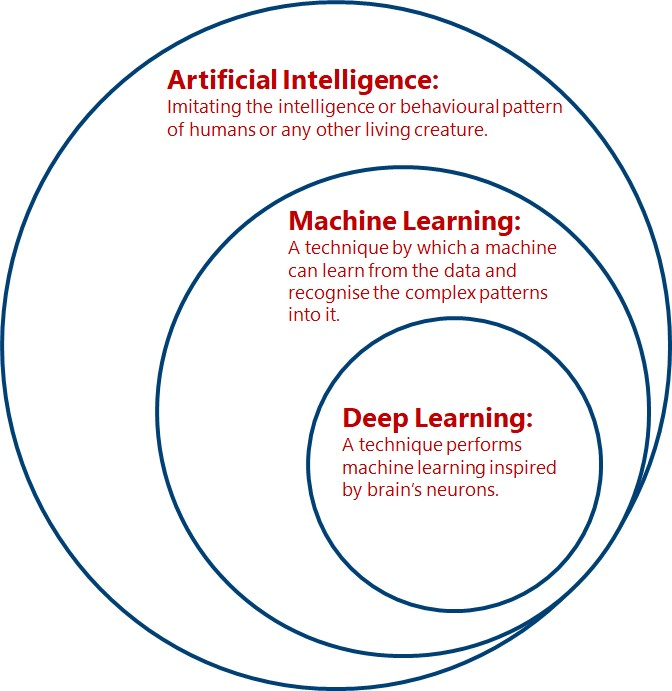
\includegraphics[scale=0.25]{images/Introduction/deeplearningsubset.jpg}
	    \caption[Relationship between Artificial Intelligence, Machine Learning, and Deep Learning.]{Relationship between Artificial Intelligence, Machine Learning, and Deep Learning.}
	    \label{fig:deepLearningSubset}
	    \end{center}
\end{figure}


The concept of deep learning was invented as early as the 1950s, although it was largely ignored until the 1980s and 1990s. However, with the efficient, fast computation hardware, and abundant data since decade it has become a popular research topic among many \ac{AI} research institutions, organizations, and startups. Deep learning is inspired by the biological network of neurons present inside the brain. Deep learning algorithms learn to discover meaningful, complex patterns in the digital representation of data, like sounds and images. To achieve this, deep learning uses a multi-layered structure of algorithms called Artificial Neural Networks (\acp{ANN}). \acp{ANN} are the heart of deep learning. They are flexible, efficient, and scalable, and suitable for vast and highly complex deep learning tasks like classifying billions of images (e.g., Google Images, Instagram, and Facebook), object detection (e.g., Tesla's Self-driving Cars), improving speech recognition systems (e.g., Apple's Siri, Amazon's Alexa, and Google Assistant), defense systems (Israel's Iron Dome, U.S.A's Patriot Missile System), and recommending the best videos to watch to hundreds of millions of users every day (e.g., YouTube).

Neural Networks are capable enough to solve complex problems by extracting features, recognizing patterns in data efficiently. However, there are certain challenges while training the neural networks. The two main things that can cause difficulties are bad algorithms and bad data. Let's start with some examples of bad data. Insufficient training data is one of the main problems that may arise when training deep learning models. A large amount of training data is required for most deep learning models to work properly. The second is the poor quality data. If the training data is wrong, noisy, and full of outliers, it will make it difficult for the model to detect patterns in the data. Hence the model will not perform well. The third is the irrelevant features. The model will only learn if the training data has more relevant features than irrelevant features. 

%Hence, it is often worth putting effort and spend time cleaning up training data. Most of the Machine Leaning Engineers spend significant amount of time doing the same. 

Now, that after some examples of bad data, let's look at some of the examples of bad algorithms. Overfitting and underfitting are one of the main problems of deep learning. ``Overfitting happens when the model is too complex relative to the amount and noisiness of the training data''\cite{10.5555/3153997}. In the overfitting, model learns training data including noise to the extent, it negatively impacts the performance of the model, leading to higher generalization error on unseen data. One of methods used to decrease the risk of overfitting is regularization\cite{kukacka2017regularization}. Regularization is one of the solutions provided to generalize a model better to the new examples. ``Underfitting is the opposite of overfitting, it occurs when a model is too simple to learn the underlying structure of the data''\cite{10.5555/3153997}. In the case of the underfitting model, it neither learns training data nor generalize to the unseen data. The problem of underfitting is resolved ``by choosing a powerful model with more parameters and providing better features during the model learning process''\cite{10.5555/3153997}. The training of the deep learning model is highly influenced by the quality and quantity of the data that has been used for the training. But in many cases, data is scarce and it is very difficult to have data that is labeled and annotated.


%In the following sections, the motivation behind this thesis is discussed in section \ref{motivation} and the problem statement is discussed in section \ref{ProblemStatement}. The objectives of this thesis discussed in section \ref{thesisobjectives}. The thesis structure and limitations are discussed in section \ref{thesisstructurelimitations}. Finally, the terminologies used in this thesis are defined in section \ref{terminology}.



\section{Motivation}\label{motivation}

Deep learning methods have many effective applications in several fields, including natural language processing and computer vision. However, these methods still are limited by poor generalization due to the insufficient quantity of training data\cite{8978087}. Annotated data are scarce when it comes to developing deep learning models for computer vision applications. The performance of such deep learning models can be improved with the introduction of a large amount of annotated data. However, due to the high cost of data annotation, it is difficult to obtain a large set of annotated training data, especially when there are many classes of data. To overcome the obstacle of the scarcity of annotated data, there are some methods available to tackle this problem. The popular methods are Active Learning\cite{hemmer2020deal}, Data Augmentation\cite{Shorten.2019}, Transfer Learning\cite{zhuang2020comprehensive}, and Domain Adaptation\cite{redko2020survey}. 

\begin{figure}[H]
        \begin{center}
 	    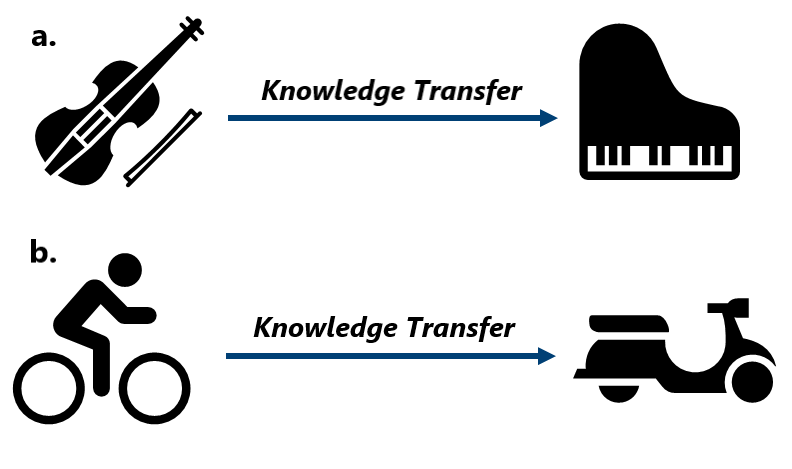
\includegraphics[scale=0.40]{images/Introduction/TransferLearning.png}
	    \caption[Simple examples of transfer learning.]{Simple examples of transfer learning.}
	    \label{fig:TransferLearning}
	    \end{center}
\end{figure}

This thesis aims to solve the data scarcity problem using the domain adaptation method. Domain adaptation is a subcategory of transfer learning in which the task is to transfer the knowledge from the source domain to the target domain. ``Transfer learning is the ability of a system to recognize and apply the knowledge learned from one task to another task''\cite{zhuang2020comprehensive}. For example, if a person has mastered one musical instrument like the violin, can learn piano faster compared to others, as the knowledge of one musical instrument can be applied while learning another musical instrument. Figure \ref{fig:TransferLearning} shows an intuitive example of transfer learning. Transfer learning inspired by human behavior, humans beings are capable to transfer knowledge from one domain to another domain. The transfer learning grasps knowledge from the source domain to improve the learning performance in the target domain so the number of labeled samples required in the target domain can be reduced. It is important to mention, transfer learning is effective only if the source domain and target domain are related. For example, learning bicycles will not help to learn piano faster. Qiang Yang et al.\cite{5288526} have performed survey on transfer learning, more information about the transfer learning can found in their research paper.  

When the source and target domains are the same and learning tasks also the same, then such a learning problem becomes a traditional machine learning problem\cite{5288526}. When the source and target domains are different but related, and learning tasks are the same then, such a learning problem becomes a domain adaptation problem\cite{5288526}. In domain adaptation, source and target domains have the same feature space but different distributions in contrast to transfer learning, which includes cases where the target domain's feature space is different from the source domain's feature space\cite{5288526}. Domain adaptation is distinguished depending upon the similarity or dissimilarity of feature space and availability of annotated data in the source domain and target domains. The domain adaptation has two categories, if the feature space is the same between the source domain and target domain is called homogeneous domain adaptation. If the feature space is different between the source and target domain is called heterogeneous domain adaptation. Further homogeneous and heterogeneous domain adaptation divided into three types of domain adaptation, supervised domain adaptation, semi-supervised domain adaptation, and unsupervised domain adaptation. In the supervised domain adaptation, the samples in the target domains are labeled. Semi-supervised domain adaptation has a small set of labeled and unlabeled samples in the target domain. And, in unsupervised domain adaptation, the samples in the target domain are not labeled\cite{5288526}. A simple example of domain adaptation of  \ac{SVHN} transformed into handwritten digits shown in figure \ref{fig:DA}. The difference between traditional machine learning and domain adaptation is shown in figure \ref{fig:DomainAdaptation}.


\begin{figure}[H]
        \begin{center}
 	    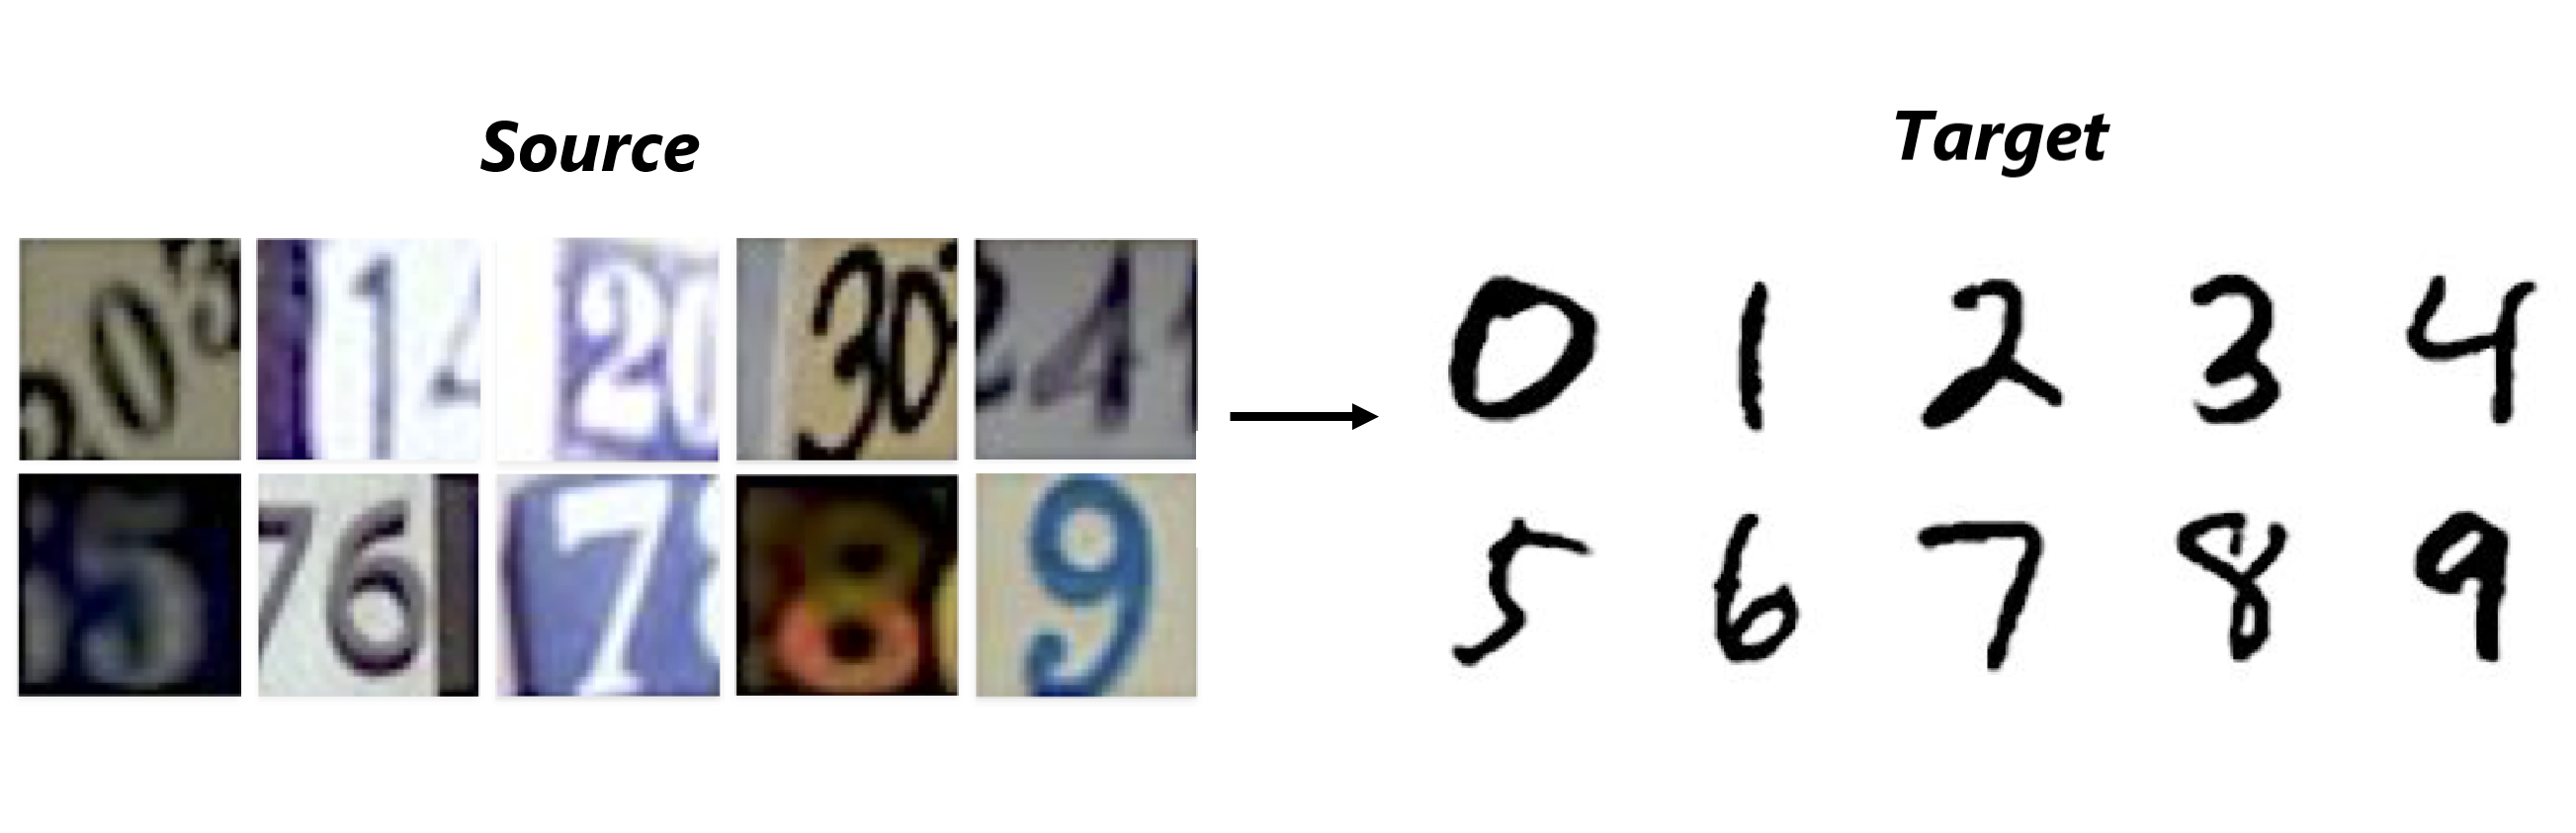
\includegraphics[scale=0.15]{images/Introduction/DA.png}
	    \caption[Simple example of domain adaptation from \ac{SVHN} dataset to \ac{MNIST} Dataset for the digit recognition task.]{Simple example of domain adaptation from \ac{SVHN} dataset\cite{37648} to \ac{MNIST} Dataset\footnotemark for the digit recognition task.\footnotemark}
	    \label{fig:DA}
	    \end{center}
\end{figure}
\footnotetext[1]{\url{http://yann.lecun.com/exdb/mnist/} last access: \dcdate}
\footnotetext[2]{\url{https://machinelearning.apple.com/research/bridging-the-domain-gap-for-neural-models} last access: \dcdate}





To understand how domain adaptation works, let's have a simple example. Consider the source domain represented by the \ac{SVHN} dataset. It is a collection of house number images, and the target domain is represented by the \ac{MNIST} dataset, which is a collection of handwritten digits images. When the \ac{CNN} is trained and evaluated on the source domain \ac{SVHN} dataset for the task of identifying numbers, it will achieve high accuracy. However, the same classifier will perform worst when evaluated the\ac{MNIST} dataset. This performance gap occurs due to differences between the domain data distribution. The images in the \ac{SVHN} dataset consist of different fonts, blur, noise, and different backgrounds. But the images in the \ac{MNIST} dataset contain a clean background and handwritten strokes. Now consider images are scarce in the target domain. Only a small amount of the target domain images are available, which are unlabeled. As we know training a classifier using a smaller amount of data leads to underfitting and eventually leads to the worst performance on unseen data. Hence, to create a sufficient amount of data, the domain adaptation model is trained. It learns to transfer the underlying knowledge from the source domain to the target domain. In this case, labeled data is available in the source domain, and unlabeled data available in the target domain. Such a setup is called unsupervised domain adaptation because the model learns to transform images from one domain to another in the absence of labeled data in the target domain, and without taking much help from the labeled data from the source domain during the learning process. Using this domain adaptation model, large amount of annotated data can be created in the target domain by transforming source domain images into target domain images. Once a sufficient amount of images present in the target domain, the task to identify numbers in the target domain can be improved significantly. Nowadays, the domain adaptation technique is widely used in the field of \ac{HTR}\cite{Kang_2020}, Image Classification\cite{5288526}, Style Transfer\cite{johnson2016perceptual}, and \ac{OCR}\cite{8978011} to solve the problem of scarcity of data. Making such applications robust, accurate, and efficient is a big task, which requires years of research. The scope of this thesis is limited to improving document image classification using the proposed domain adaptation technique.

\begin{figure}[H]
        \begin{center}
	    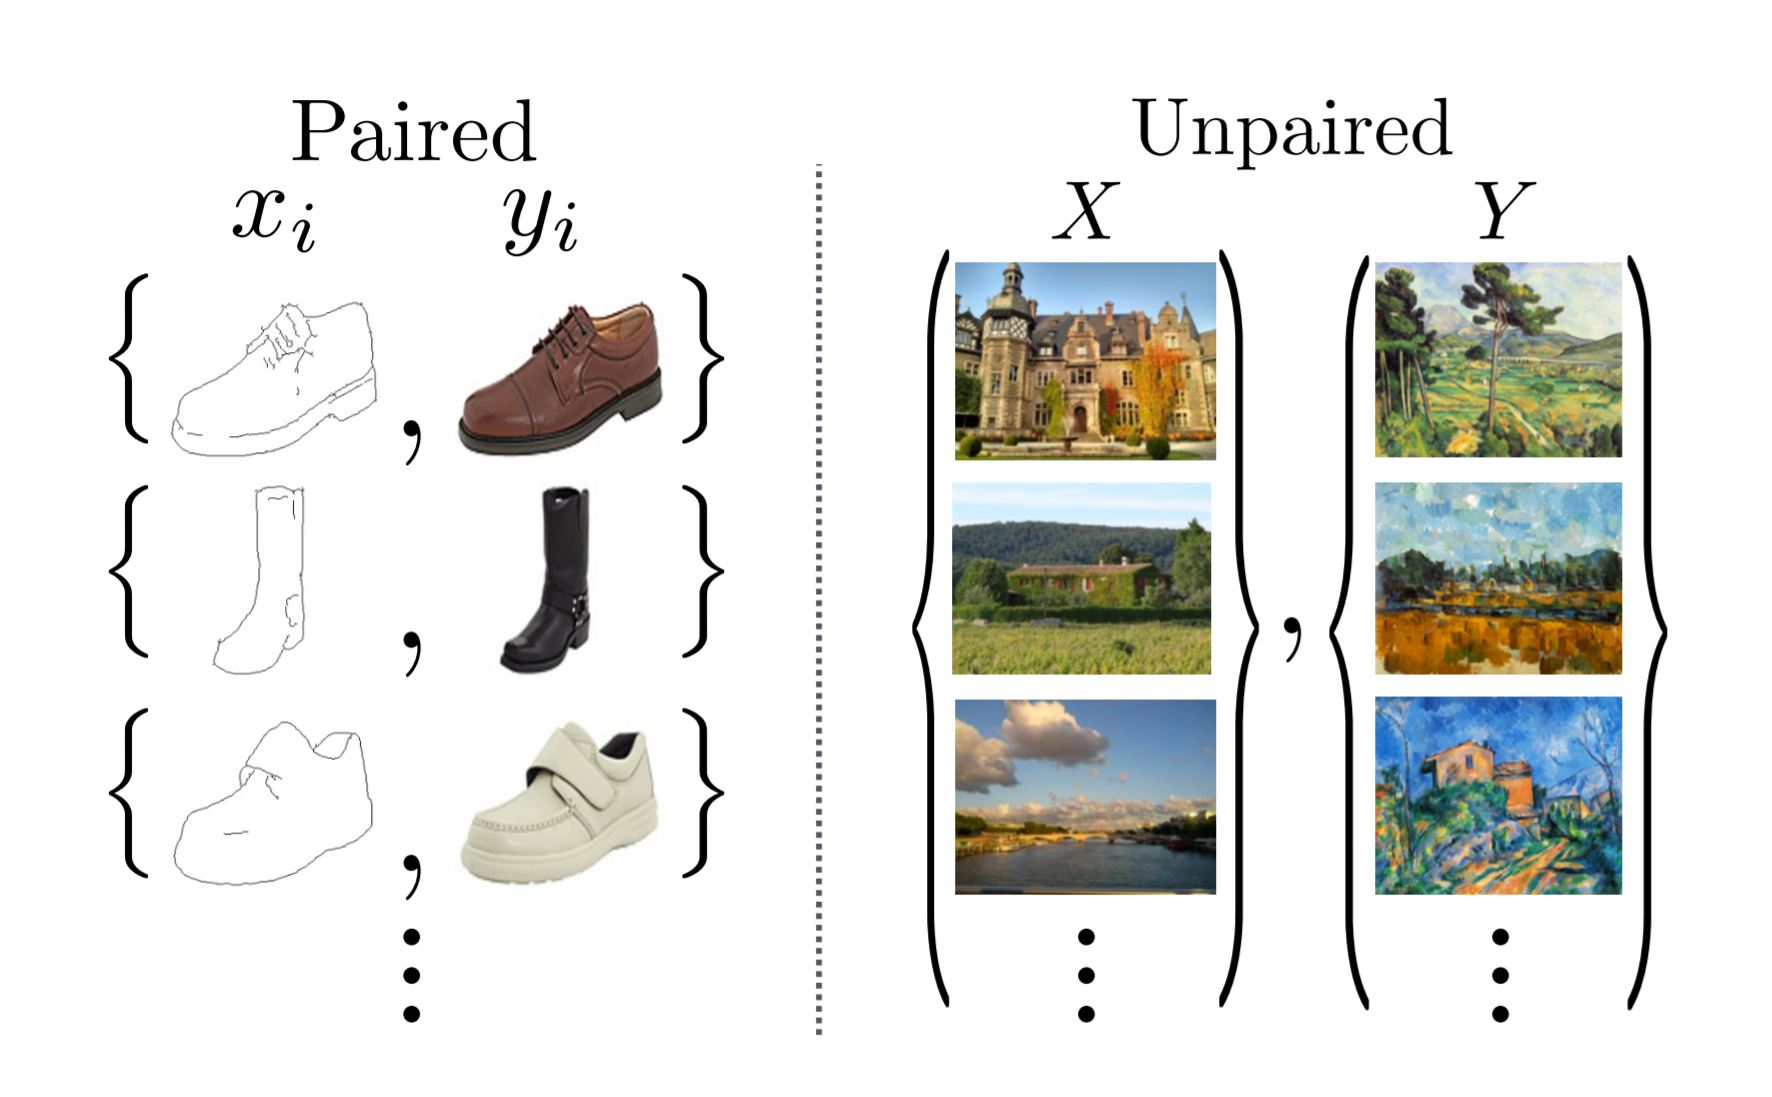
\includegraphics[scale=0.50]{images/Introduction/img_translation.JPG}
	    \caption[Examples of the paired training data set and the unpaired training data set.]{The paired training data set consists of training examples, in which there is a correspondence between the source domain and the target domain (Left, Edges $\leftrightarrow$ Images). But in the unpaired training data set, there is no correspondence between the source domain and the target domain (Right, Photographs $\leftrightarrow$ Painitings)\cite{zhu2020unpaired}.}
	    \label{fig:img_translation}
	    \end{center}
\end{figure}


\begin{figure}[H]
        \begin{center}
	 	    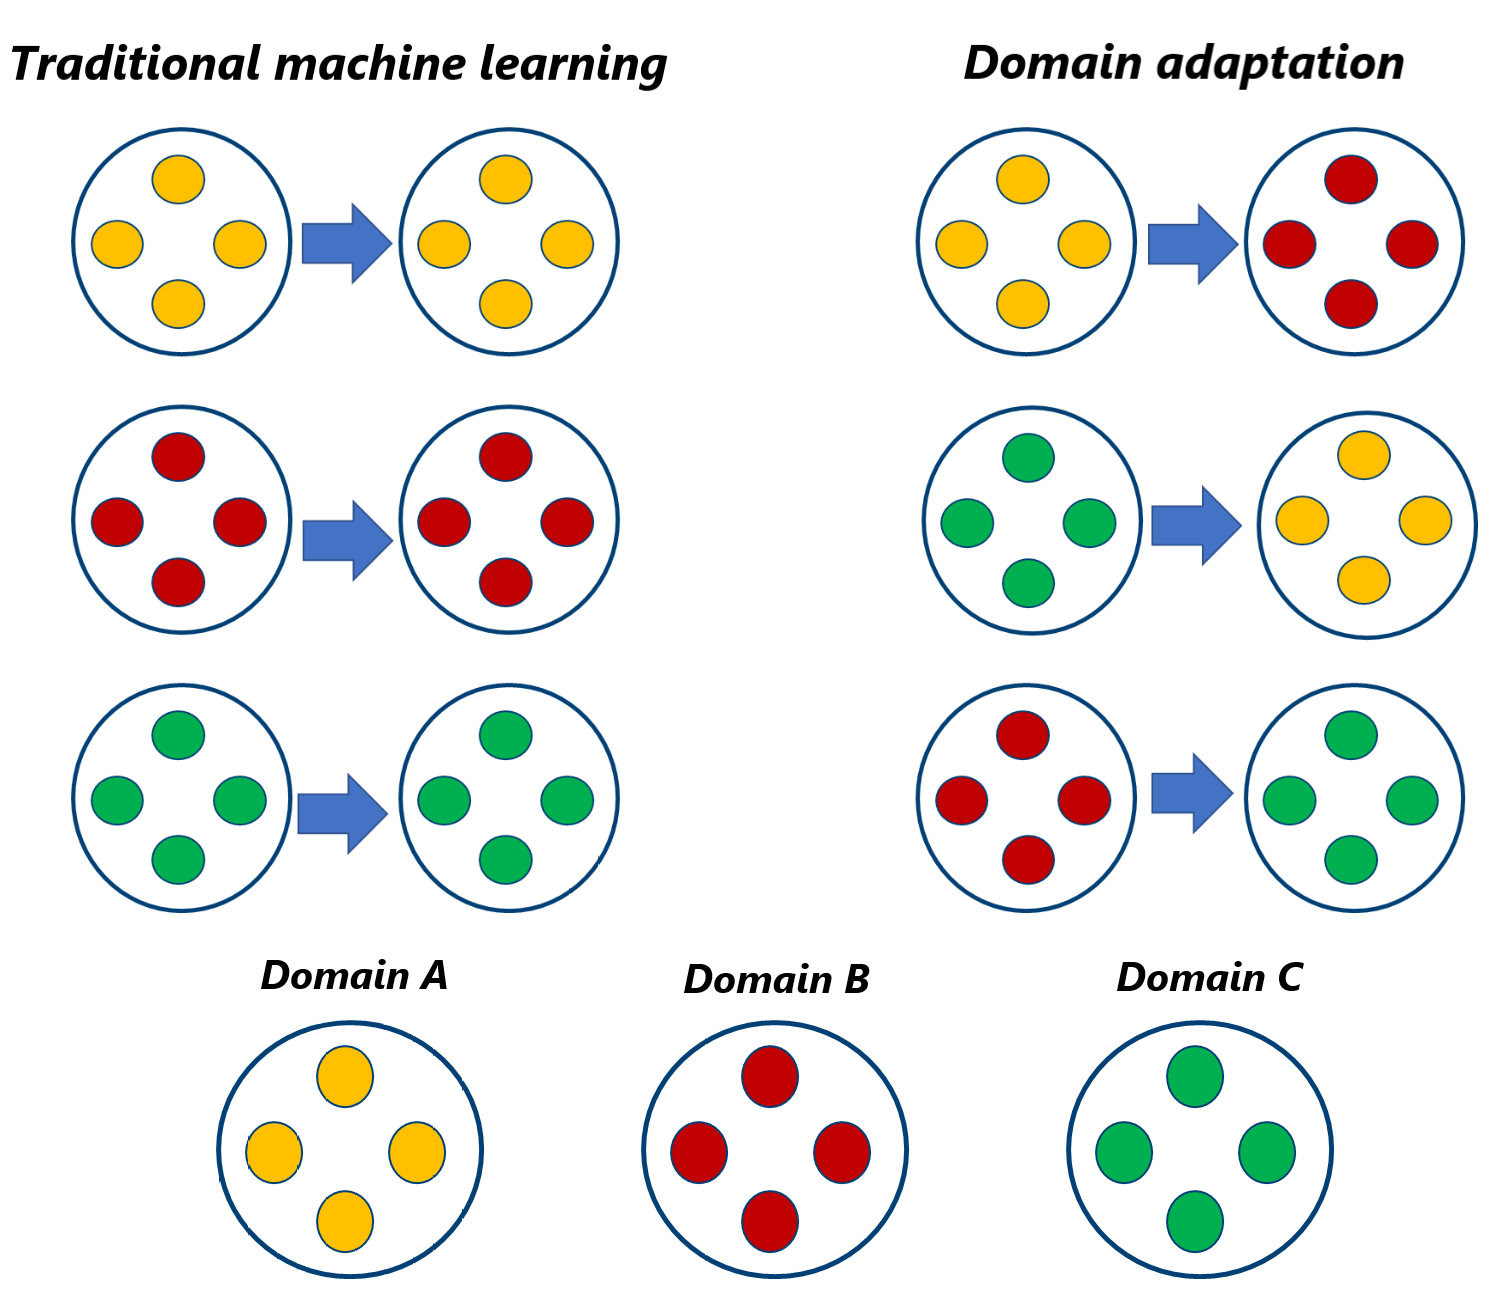
\includegraphics[scale=0.28]{images/Introduction/DomainAdaptation.png}
	    \caption[Difference between traditional machine learning and domain adaptation.]{Difference between traditional machine learning and domain adaptation.}
	    \label{fig:DomainAdaptation}
	    \end{center}
\end{figure}




\section{Problem Statement and Proposed Solution}\label{ProblemStatement}

As described earlier, a large amount of data is required to train a neural network, but annotated data is scarce, and data labeling is a costly and tedious job. For example, in this thesis, it is being addressed that collecting several and distinct real document images (figure \ref{fig:RealImage}) with different types of handwriting is expensive and difficult job. In such cases, machine learning engineers have to inevitably generate synthetic document images. However, deep learning models trained using synthetic document images will not generalize well on unseen real document images\cite{8978087} (figure \ref{fig:Problem}). Because, the synthetic document images lacks realism\cite{8978087}. They don't possess a similar noise distribution, characteristic, and artifacts as real document images\cite{8978087}. Hence, in the last two decades, numerous domain adaptation methodologies have been introduced to perform image-to-image translation\cite{8978011}. Image-to-image translation is a method of transforming images from source to a target domain by learning the underlying characteristic of target domain images. It is used to transform synthetic images into realistic images by reducing the divergence or gap between the distribution of real data and the distribution of synthetic data. In this thesis, an image-to-image translation application is developed using \ac{CycleGAN} to reduce the domain gap between synthetic data distribution and real data distribution\cite{zhu2020unpaired}. The \ac{CycleGAN} is an extended variant of Generative Adversarial Network (\ac{GAN})\cite{goodfellow2014generative}. It is a method to perform unpaired image-to-image translation, in which the model is trained using the collection of images from the source and target domain that are not related to each other\footnotemark.
\footnotetext{\url{https://machinelearningmastery.com/what-is-cyclegan/} last access: \dcdate}


The proposed image-to-image translation application is developed in consultation with, \ac{ML} developers at Elevait Deutschland GmbH, a Germany-based company that develops \ac{AI} applications for business use-cases. Elevait is widely contributing in the field of Cognitive Business Robotics\cite{Metta2012} to automate document processing. Elevait has developed state-of-the-art \ac{HTR} and \ac{OCR} tools to process documents and extract information from them. To make those systems robust and efficient, a large number of document images are required. The idea is to create a large number of synthetic document images to have a large quantity of annotated data. However, as mentioned earlier, the synthetic document images will not generalize well when they have to process real document images because real document images have different characteristics. Furthermore, real document images possess artifacts such as salt-and-pepper, background noise, blur due to camera motion or shake, watermarks, stains, wrinkles, and fading text, introduced during the scanning process\cite{sharma2019learning}. To address this problem, in this thesis, the image-to-image translation application is developed to transform synthetic document images into realistic document images to reduce the domain gap between real data distribution and synthetic data distribution. In this way, a large number of realistic document images can be generated to reduce the scarcity of annotated real document images in the target domain.




\begin{figure}[H]
        \begin{center}
	    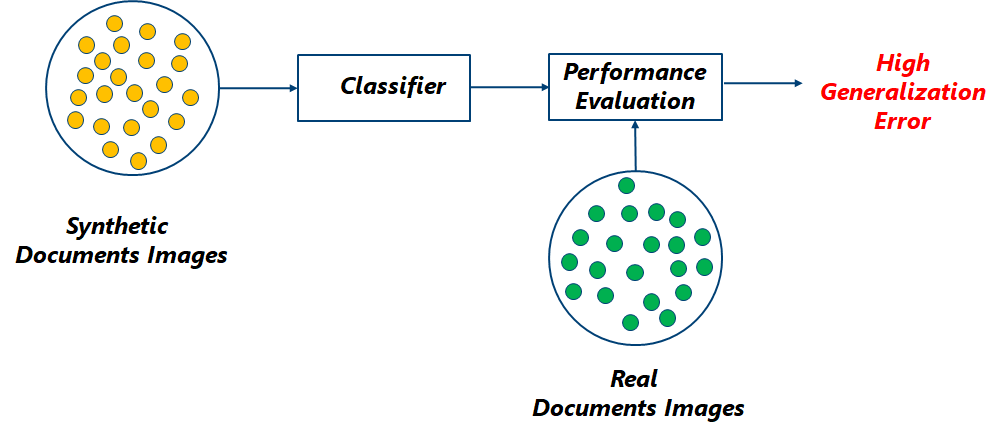
\includegraphics[scale=0.60]{images/Introduction/Problem.png}
	    \caption[An illustration of the problem to be solved in this thesis.]{An illustration of the problem to be solved in this thesis.}
	    \label{fig:Problem}
	    \end{center}
\end{figure}



The synthetic document images are created using templates (figure \ref{fig:template}) and handwritten crops (figure \ref{fig:keinwifi}) retrieved from handwriting datasets like \ac{MNIST} (figure \ref{fig:handwrittenCrops}) or any other datasets. These templates contain fields like are customer number, customer name, and other customer information. These fields are represented by using bounding boxes. The bounding boxes are annotated using \ac{COCO} annotations\cite{10.1007/978-3-319-10602-1_48}. The handwritten crops are inserted over the empty templates to generate numerous synthetic document images. The proposed image-to-image translation application solves the following problems. First, labeled synthetic document images are available in the source domain, ultimately, using the proposed application the collection of synthetic document images are transformed into realistic document images in the target domain. So the problem of labeling, annotations, and scarcity is solved. Second, consider, a huge chunk of real document images are not labeled. If the simple classifier is trained on realistic document images. Later, these chuck of real document images can be automatically classified with ease. This will save data annotation and data collection efforts. Further, making image classification tools in the target domain robust and efficient even in the absence of real data. The figure \ref{fig:Problem} describes if the classifier is trained using synthetic document images, it won't generalize well on the unseen real document images. Further, it leads to high generalization error, hence represented in dark red color for better understanding. In figure \ref{fig:ProposedSolution} Data distribution in light green color represents realistic document images which is generated by the proposed image-to-image translation application. Dark green represents the real document images.  Further, the classifier is trained using realistic document images, generalizes better on the unseen real document images compared to the classifier are trained using synthetic document images, hence low generalization error represented in light red color for better understanding when compared to figure \ref{fig:Problem}.



\begin{figure}[H]
        \begin{center}
	    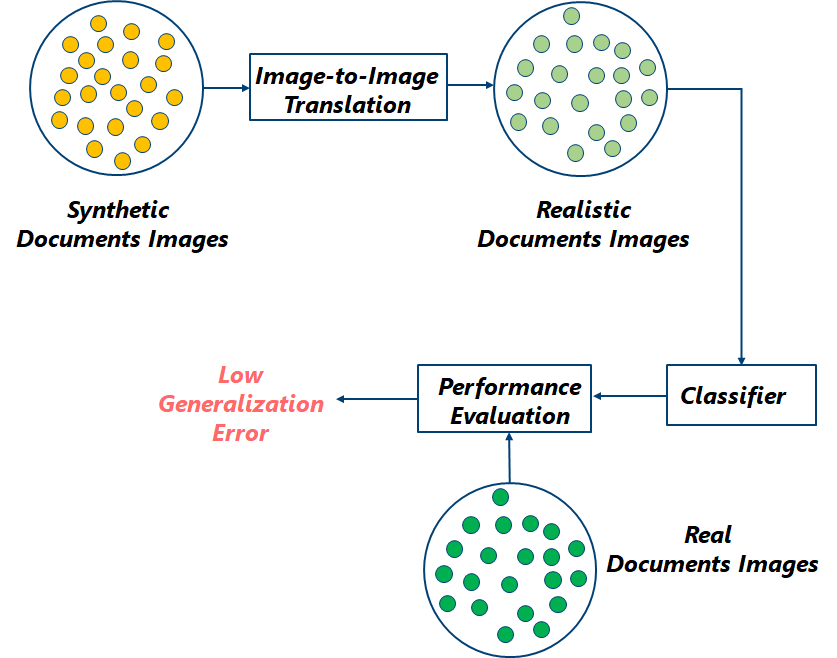
\includegraphics[scale=0.55]{images/Introduction/ProposedSolution.png}
	    \caption[An illustration of the solution proposed to reduce the domain gap between the synthetic document images and the real document images.]{An illustration of the solution proposed to reduce the domain gap between the synthetic document images and the real document images.}
	    \label{fig:ProposedSolution}
	    \end{center}
\end{figure}

\newpage

\section{Thesis Objectives}\label{thesisobjectives}
The goal of this thesis is to close the domain gap between synthetic data distribution and real data distribution by developing an image-to-image translation application using \ac{CycleGAN}, which is used to transform synthetic document images into realistic document images. In addition, in this thesis, experiments are conducted to understand the domain gap between data distributions. The main objectives of this thesis are listed below:
%Every research work has its own objectives.
\begin{enumerate}
\item Conduct a literature survey, in which different types of image-to-image translation methods are discussed and briefly explained. In addition, also discuss a theoretical comparison between existing methods, which lead to the reason for choosing \ac{CycleGAN} to solve the problem statement. 

\item Create a dataset of synthetic document images, faxified document images, and real document images. In addition, a testing dataset of annotated real document images is collected for evaluation of the models.

\item Implement proposed image-to-image translation application using \ac{CycleGAN}. Next, train the application model using a dataset of synthetic document images and real document images. A dataset of synthetic document images represents the source domain, and a dataset of real document images represents the target domain.

\item Train three different classifiers on different data distributions (Synthetic document images, Faxified document images, and \ac{CycleGAN} generated document images) and evaluate their performance on unseen annotated real document images (testing dataset) and analyze the domain gap between these distributions and real data distribution, using metrics like accuracy, macro average f1-score, and weighted average f1-score. These experiments are listed briefly below:
	\begin{enumerate}
	     	\item Train a classifier using synthetic document images and evaluate its performance over testing dataset.
     	     	\item Train a classifier using faxified document images and evaluate its performance over testing dataset.
     		\item Train a classifier using \ac{CycleGAN} generated document images and evaluate its performance over testing dataset. This experiment helps to determine the quality of images generated by the proposed image-to-image translation application.
    	\end{enumerate}
\item Record all details regarding this thesis, for example, literature survey, selected methodology, fundamentals required to understand this thesis, implementation, experiments performed, obtained results, analysis of results, limitations and scope of the research, conclusion, and future work.
\end{enumerate}


\section{Thesis Limitations and Structure}\label{thesisstructurelimitations}
The domain adaptation field is promoting incremental findings, hence this thesis has its limitations due to time constraints. The solution of the defined problem and analysis performed in this thesis investigated only using \ac{CycleGAN}. The comparison with other methodologies is kept apart for future research. The scope of this thesis is limited to the improvement of real document images classification by increasing the quality and quantity of annotated images in the target domain using the proposed image-to-image translation application. The thesis is organized as follows. Chapter \ref{relatedworks} describes related literature and existing methods to solve the problem. Chapter \ref{fundamentals} discusses essential topics \acp{GAN} and \acp{CNN}. Chapter \ref{methodology} describes the method and loss functions used to solve the defined problem. Chapter \ref{implementation} describes the details about the dataset, the architecture of the neural networks implemented in this thesis. Chapter \ref{evaluation} illustrates the evaluation metrics, experiments performed, and obtained results. Chapter \ref{conclusion} concludes the research and results analysis along with the future work and the limitations of the thesis.





%The scope of this thesis is limited to the improvement of real document images classification by increasing the quality and quantity of labeled data in the target domain, and reducing the domain gap between synthetic data distribution and real data distribution. 

\begin{comment}
\section{Terminology}\label{terminology}
In this thesis for simplicity and readability, many terms are explained beforehand for better understanding and to avoid confusion. The following terms described in this thesis are consistently used throughout this thesis. The term ``Artificial Neural Networks'' will be used as ``Neural Networks'' interchangeably. The images generated by the \ac{CycleGAN} generator in the target domain are called ``Realistic Document Images'' and they are also interchangeably called ``\ac{CycleGAN} Generated Document Images''. So, the distribution of ``\ac{CycleGAN} Generated Document Images'' is called ``\ac{CycleGAN} Generated Data Distribution''.
\end{comment}









%%%%%%%%%%%%%%%%%%%%%%%%%%%%%%%%%%%%%%%%%%%%%%%%%%%%%%%%%%%%%%%%%%%%%%%%%%%%%%%%%%%%%%%%%%%%%%%%%%%%%%%%%%%%%%%%%%%%


%The proposed application model is trained to capture the characteristics of real document images and transform an image from the source domain to the target domain. Such a kind of transformation is called image-to-image translation.

%In this thesis, the handwritten crops are inserted over the templates to generate numerous synthetic document images. 
%As mentioned earlier deep learning models trained using synthetic document images will not generalize well on real document images.
%As mentioned earlier deep learning models trained using synthetic document images will not generalize well on real document images. Further, the image-to-image translation application is developed using \ac{CycleGAN} to transform synthetic document images into realistic document images. ultimately, to reduce the domain gap between synthetic data distribution and real data distribution. 
%A large number of realistic document images can be generated to tackle the problem of data scarcity in the target domain. As we already know that real document images are scarce and labeling images is a tedious and costly job. 
% The proposed image-to-image translation application transforms synthetic document images to realistic document images to solve the following problems. 
%The proposed solution is to use domain adaptation methods like the image-to-image translation to reduce the divergence between data distributions.


%The handwriting datasets and document images datasets are can not be disclosed or cited due to data privacy concerns and copyright issues.
%By comparing a classifier performance on real data distribution by first training them on data distributions like synthetic data, faxified data, and \ac{CycleGAN} generated data. 






%Every research work comes with definite objectives to achieve. The Objective 1 of the thesis is to perform a literature survey, in which, different types of image-to-image translation methods should be discussed. Furthermore, the theoretical comparison between existing methods must be discussed, to finally decide a methodology to solve the problem statement. Objective 2 is to create and collect datasets to train neural networks by keeping small testing aside to evaluate models. Objective 3 is to proceed with the design and development of the neural networks during the implementation phase of this thesis. Objective 4 is to perform experiments, and Objective 5 is to analyze, evaluate results achieved by the chosen method, implementation. Objective 6 is to document all the information regarding the thesis, for example, chosen methodology, fundamentals required to understand the work, experiments, results, limitations, conclusion, and future work.


%during the implementation phase of this thesis. In this step the \ac{CycleGAN} is implemented and trained.

\begin{comment}
The neural networks trained in this thesis using images of resolution $256 \times 256$. In the real world, document images are of higher resolution.
\end{comment}

\begin{comment}
The \ac{CycleGAN} is used to transform synthetic document images into realistic document images as \acp{CycleGAN} is the state-of-the-art for unpaired image-to-image translation. This image-to-image translation application deals with synthetically generated document images, which are created using empty template images and handwritten crops retrieved from data sets like \ac{MNIST} or any other data sets. The dataset used in the thesis is copyrighted, which can not be exposed to public use. Handwritten crops are pasted over the empty template images to generate numerous synthetic document images. Nevertheless, deep learning models trained using synthetic document images will not generalise well on real document images. Hence, the \ac{CycleGAN} is used to perform the unpaired image-to-image translation and transform synthetic document images into realistic document images.
\end{comment}




\begin{comment}
This thesis starts with Objective 1, Literature Survey, in which, different types of image-to-image
translation methods are discussed. Also, it addresses how general GANs are extended by modifying
their objective function to solve different kinds of image-to-image translation problems. General
GANs suffers from mode collapse, literature survey helped to find the efficient and easy solution
to overcome such problems. Furthermore, the theoretical comparison between existing methods
has discussed, ultimately deciding a methodology to solve the problem statement. Objective 2,
the creation of datasets is an important aspect of training any neural network. The datasets for
synthetic document images, faxified document images have been created. Also, a large chunk of
unlabeled real document images is collected. A small testing dataset of real document images is
kept aside to evaluate models. Objective 3, once the dataset was ready, the software development
was carried out during the implementation phase of this thesis. Objectives 4 and 5, experiments
were performed to analyze whether the chosen method, implementation, and approach produced
acceptable results, and all the results were recorded for evaluation. Objective 6, was the challenging
phase, all the information regarding this thesis, for example, chosen methodology, fundamentals
required to understand the work, results, and conclusion of the thesis has been written in a report
for submission.
\end{comment}


\begin{comment}
The architecture of \ac{CycleGAN} is adapted from Johnson et al. ~\cite{johnson2016perceptual}. The generator network is implemented using a sequence of downsampling convolutional blocks to encode the $256 \times 256 \times 1$ grayscale input image, 9 \ac{ResNet} convolutional blocks to transform the image, and a number of upsampling convolutional blocks to generate the output image of the same dimension as the input image. The reason behind using residual blocks is it resolves the vanishing gradient problem in deep neural networks. The discriminator networks uses PatchGAN ~\cite{isola2018imagetoimage}. In PatchGAN, after feeding one input image to the network, it gives you the probabilities of two things: either real or fake, but not in scalar output indeed, it used the $N \times N$ output vector. Here $N \times N$ can be different depending on the dimension of an input image. The architecture of both generator and discriminator networks will be thoroughly discussed in Chapter \ref{implementation}. To evaluate the quality of images generated by the \ac{CycleGAN}, a classifier is trained on the \ac{CycleGAN} generated data and its accuracy on a real test set is used as a metric to measure how well the \ac{CycleGAN} model distribution matches the real data distribution. Basically, The classification capability of the trained classifier is used as an objective measure to assess the quality of images generated by \ac{CycleGAN}. 
\end{comment}







\begin{comment}
\begin{figure}[H]
        \begin{center}
	    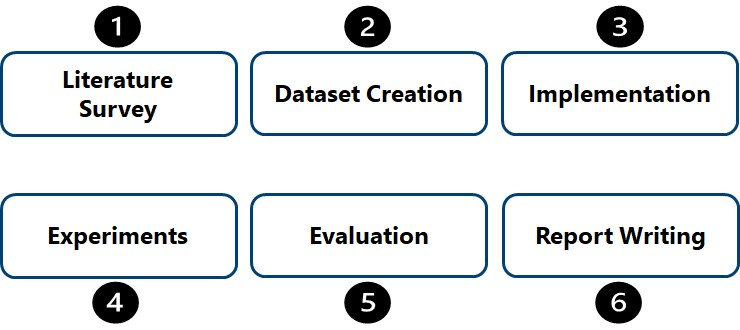
\includegraphics[scale=0.50]{images/ThesisObjectives2.JPG}
	    \caption{Thesis Objectives.}
	    \label{fig:ThesisObjectives}
	    \end{center}
\end{figure}

\end{comment}


\newpage

\chapter{Related Works}
    \label{relatedworks}
    
%\noindent
\justifying
\setlength{\parskip}{1em}


In the last decades, the field of computer vision and computer graphics has made a tremendous amount of progress, especially in the field of domain adaptation. The image-to-image translation is a popular and classic example of domain adaptation, in which the goal is to learn the mapping between a source image and a target image using a training set of aligned image pairs \cite{mirza2014conditional}. \acp{GAN} were among the initial methods used to perform image-to-image translation \cite{pang2021imagetoimage} \cite{goodfellow2014generative}. But, \acp{GAN} suffers from unstable learning and mode collapse \cite{thanhtung2020catastrophic}. Also, for many tasks, aligned or paired training data will not be available, collecting and annotating paired document images is tedious, difficult, time-consuming and costly. Hence, over the years, several supervised and unsupervised image-to-image translation methods are developed. This chapter discusses some of those popular image-to-image translation methods. Also, a brief theoretical comparison of these existing methods is discussed. The motivation behind selecting the approach to solve the addressed problem statement of this thesis is summarized in section \ref{rwsummary}.



\section{Literature Survey}\label{LiteratureSurvey}


Ian J. Goodfellow et al.\ \cite{goodfellow2014generative} proposed a framework of \acp{GAN} in which two models are simultaneously trained. A generative model is trained to learn the data distribution and a discriminative model that predicts the probability that a sample came from the training data rather than a generative model. The idea of training a generative model is to generate realistic data and maximize the probability of a discriminative model making a mistake. The generator learns to generate realistic data and the discriminator learns to distinguish real data from the generator's fake data. The generator is penalized by the discriminator for producing non-credible results. As training starts, the generator begins to create fake data and the discriminator quickly learns to classify that it's fake and the generator is penalized to improve and produce credible results. The generator gets closer to producing output samples that can fool the discriminator as training progresses. Finally, if generator training goes well, the discriminator becomes worse at distinguishing between real and fake samples.  At the end of the training, ultimately, we have a generator model which produces credible results which are similar to real data \cite{goodfellow2014generative}. Authors have trained \ac{GAN} on a range of datasets including MNIST \cite{726791}, Toronto Face Database (TFD) \cite{susskind2010toronto} and CIFAR-10 \cite{krizhevsky2009learning}, also compared against existing methods like \ac{DBN} \cite{bengio2012better}, \ac{Stacked-CAE} \cite{bengio2012better} and \ac{Deep-GSN} \cite{bengio2014deep}. The authors do not claim that the samples generated by \acp{GAN} are better than samples generated by already existed methods \cite{goodfellow2014generative}. Authors believe at least the obtained results are competitive when compared with the better generative models in the literature, which highlights the potential of the generative adversarial framework \cite{goodfellow2014generative}. The first and foremost advantage of \acp{GAN} is computational when compared to other generative models. Adversarial models may have added statistical advantage from the generator network being updated by the gradients flowing through the discriminator using backpropagation, not being updated directly with data examples \cite{goodfellow2014generative}. Backpropagation is an algorithm to calculate gradients of the loss function to update weights of the neurons in the neural network \cite{goodfellow2017deep}. Authors metioned, to prevent the Helvetica Scenario \cite{manisha2019generative}, special care must be taken while training the \acp{GAN}. The generator must not be trained too much without updating the discriminator, training of both models should happen simultaneously. The discriminator must be updated well to provide maximum error to update the generator to produce high-quality images. Usually, \acp{GAN} should produce a wide variety of outputs. In the Helvetica Scenario, the generator collapses, repeatedly producing the same output or a small set of outputs. The Helvetica Scenario is also called Mode Collapse \cite{thanhtung2020catastrophic}.

\begin{figure}
        \begin{center}
 	    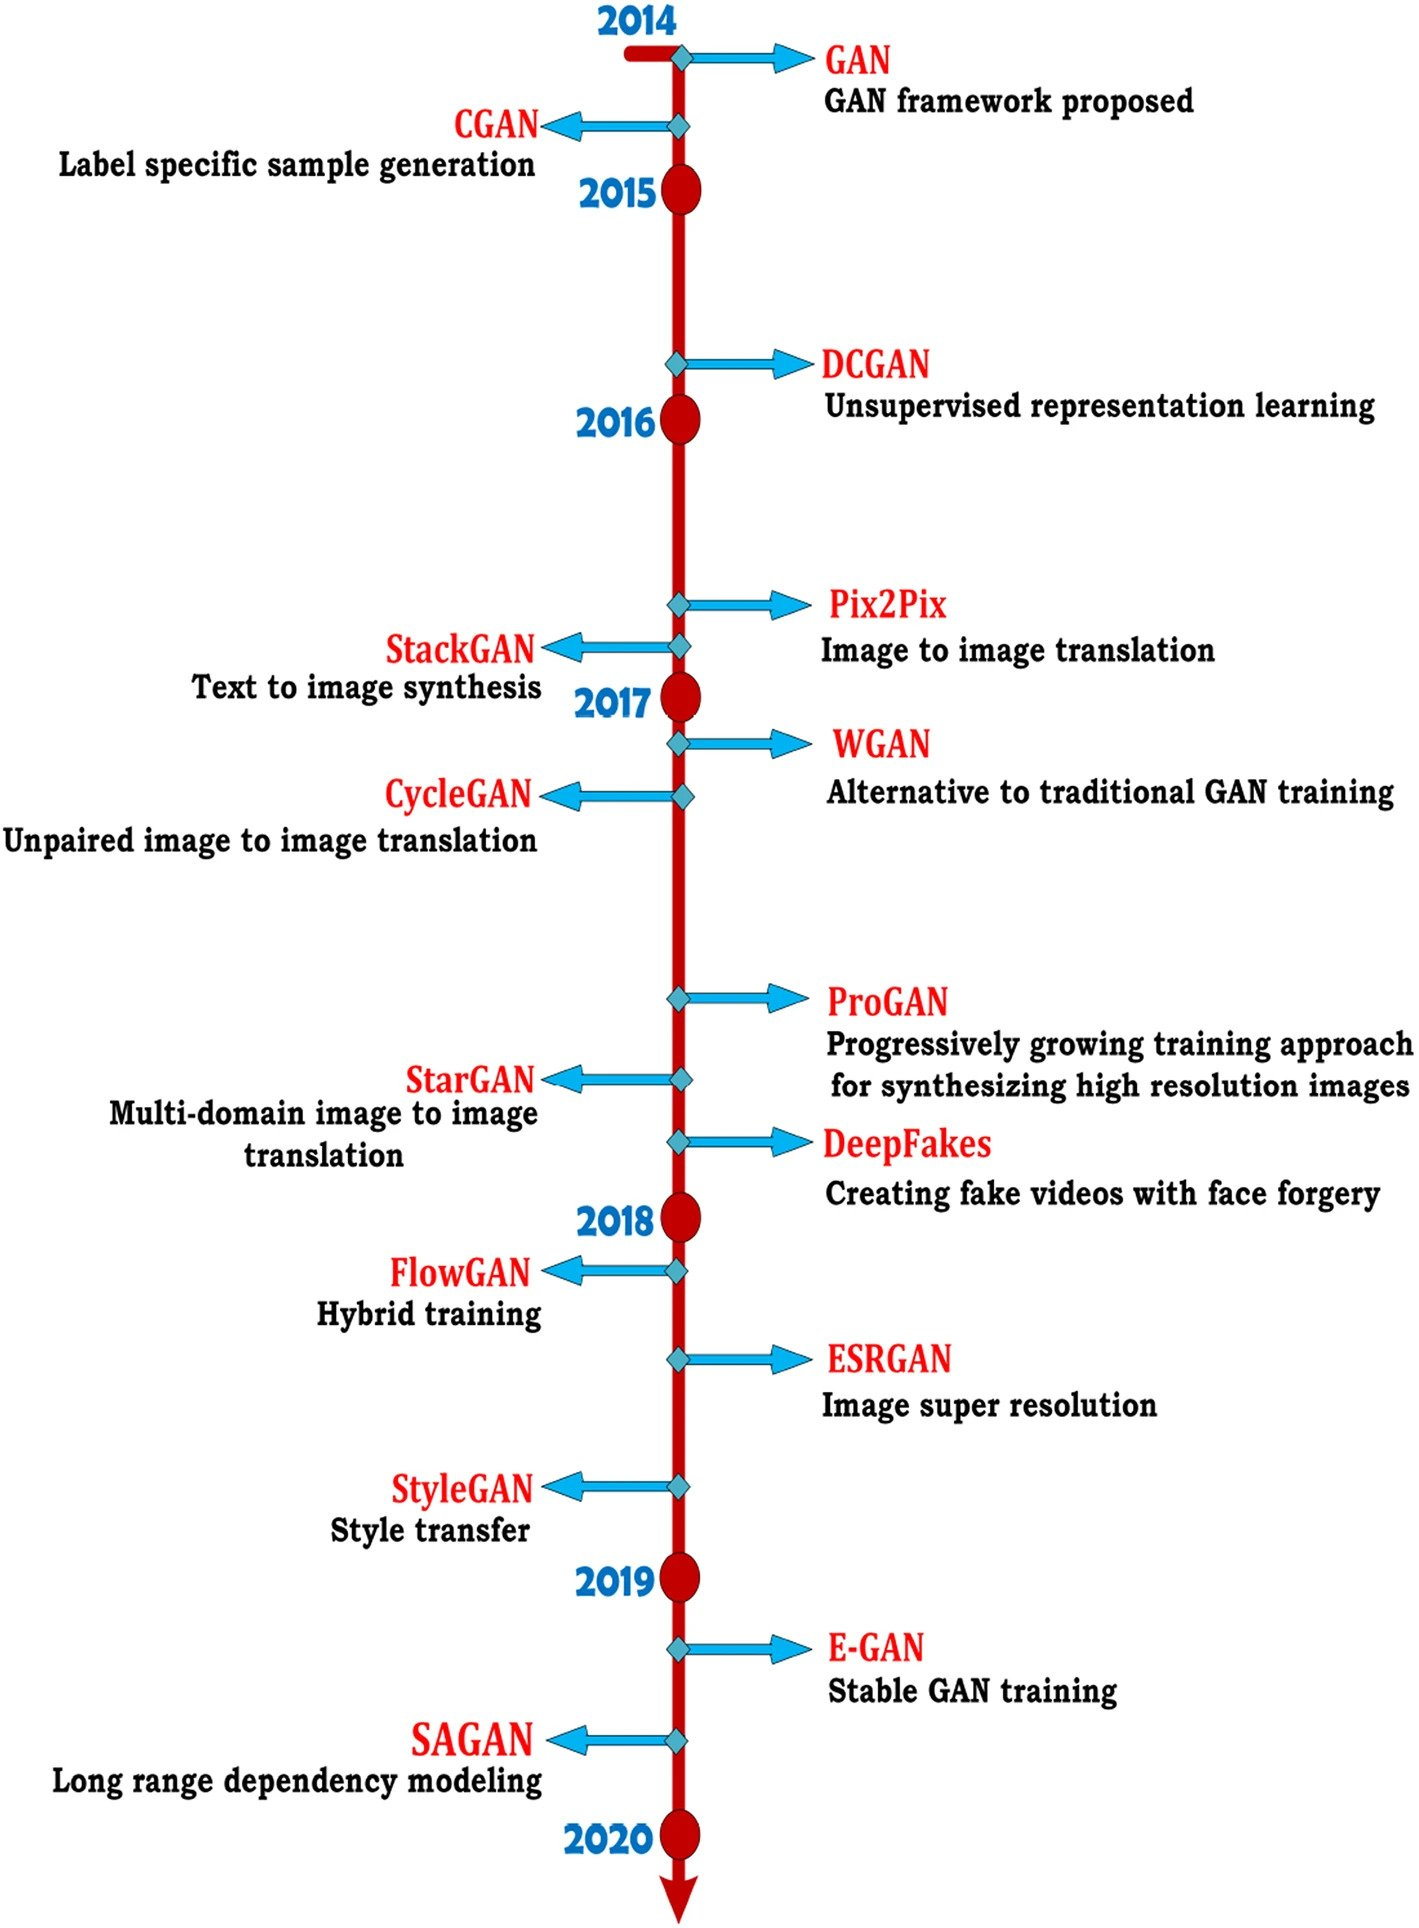
\includegraphics[scale=0.25]{images/relatedWorks/GANEvolution.jpg}
	    \caption[Evolution of \acp{GAN} Over the Years.]{Evolution of \acp{GAN} over the years \cite{PavanKumar.2021}.}
	    \label{fig:GANEvolution}
	    \end{center}
\end{figure}

Xudong Mao et al.\ \cite{mao2017squares} proposed another variant of \acp{GAN} called \acp{LSGAN}. In regular \acp{GAN}, the discriminator is hypothesized to be a classifier with the sigmoid cross-entropy loss function \cite{mao2017squares}. They realized the cross-entropy loss function can cause vanishing gradients problems during the learning process \cite{mao2017squares}. Also, regular \acp{GAN} are unstable during the learning process. Hence, the authors proposed \acp{LSGAN} to solve the problem of vanishing gradients and instability, during the learning process. \acp{LSGAN} use the least-squares loss function in the discriminator to solve the problem of vanishing gradients. In \acp{LSGAN}, the fake samples are penalized by the least-squares loss function, which forces the generator to generate samples closer towards to the decision boundary \cite{mao2017squares}. The authors evaluated \acp{LSGAN} using two datasets LSUN \cite{yu2016lsun} and HWDB1.0 (Handwritten Chinese Character Dataset) \cite{6065551}. They discovered, when trained on the LSUN dataset \cite{yu2016lsun}, \acp{LSGAN} generates better quality images than regular \acp{GAN}, \acp{DCGAN} \cite{radford2016unsupervised} and \acp{EBGAN} \cite{zhao2017energybased}. Also, when trained on the Handwritten Chinese Character Dataset, the generated characters were readable and clear. Another experiment was conducted to evaluate the stability of \acp{LSGAN} on a Gaussian mixture distribution dataset, which is designed in literature by Luke Metz et al.\ \cite{metz2017unrolled}. In this experiment, a regular \ac{GAN} and \acp{LSGAN} trained on a \ac{2D} mixture of 8 Gaussian datasets using a simplistic architecture of both generator and the discriminator, which have three fully-connected layers \cite{mao2017squares}. ``\acp{LSGAN} learn the Gaussian mixture distribution effectively and generate a wide variety of samples, but regular \acp{GAN} suffer from mode collapse and generate the single type of samples of the data distribution'' \cite{mao2017squares} and the learning process of \acp{LSGAN} is stable compared to the regular \acp{GAN}.



Phillip Isola et al.\ \cite{isola2018imagetoimage} proposed \acp{cGAN} as a generic solution to numerous image-to-image translation problems. Authors wanted to provide a single solution for multiple types of image-to-image translation problems. \acp{cGAN} learn to map input images to output images using paired training dataset. Traditionally different loss formulations are required to solve different image-to-image translation problems, but \acp{cGAN} can be used as a common generic method to solve distinct image-to-image translation problems \cite{isola2018imagetoimage}. For example, synthesizing photos from label maps \cite{cordts2016cityscapes}, reconstructing objects from edge maps \cite{zhu2018generative} \cite{6909426} and colorizing images \cite{wesley2021colorizing}. In \ac{cGAN} the generative model uses U-Net-based architecture, the U-Net is an encoder-decoder with skip connections between mirrored layers in the encoder and decoder stacks \cite{ronneberger2015unet}. The discriminative model is constructed using a convolutional PatchGAN classifier architecture \cite{demir2018patchbased}. PatchGAN is simply a \ac{CNN} in which each overlapping patch in an image is estimated to be fake or real. It penalizes structure of an image at the scale of image patches \cite{li2016precomputed}. In \acp{cGAN}, both generative and discriminative models are conditioned on some additional information, such as input images and class labels. But unconditional \acp{GAN} are not conditioned on any auxiliary information \cite{isola2018imagetoimage}. Authors found ``L1 loss encourages less blurring compared to the L2 loss'' \cite{isola2018imagetoimage}. Also combining L1 Loss and \ac{cGAN} (L1 + \ac{cGAN}) generates better results compared to combining Unconditional \ac{GAN} and L1 Loss (L1 + \ac{GAN}). The \ac{cGAN} appears to be more effective on the problem where the output is highly detailed or photographic \cite{isola2018imagetoimage}. Authors have released \ac{cGAN} as the pix2pix software and mentioned, \ac{cGAN} has widespread applications and it can be adopted without ease, to solve different image-to-image translation problems without significant parameter modifications. The pix2pix software code is available at \href{https://github.com/phillipi/pix2pix.}{GitHub}. In figure \ref{fig:CGAN} the mapping from edges $\rightarrow$ photo transformation illustrated and both generator and discriminator are conditioned on additional information like input edge map \cite{isola2018imagetoimage}.


\begin{figure}[H]
        \begin{center}
 	    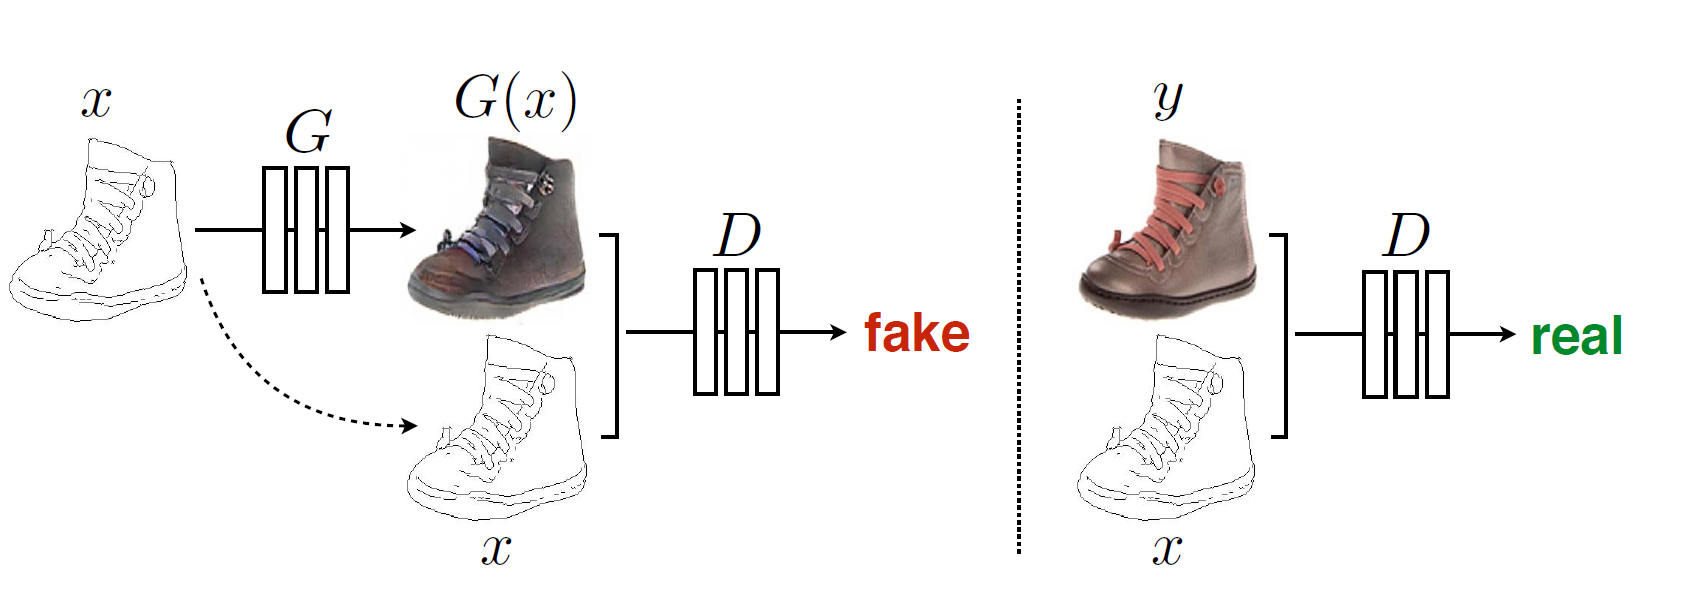
\includegraphics[scale=0.30]{images/relatedWorks/CGAN.png}
	    \caption[An illustration of training a \ac{cGAN} to map edges $\rightarrow$	 photo transformation.]{An illustration of the training a \ac{cGAN} to map edges $\rightarrow$ photo transformation. In \acp{cGAN}, both discriminator and generator observe the input edge map, unlike Unconditional \acp{GAN} \cite{isola2018imagetoimage}.}
	    \label{fig:CGAN}
	    \end{center}
\end{figure}

Taesung Park et al.\ \cite{park2020contrastive} proposed \ac{CUT} for encouraging content preservation in unpaired image-to-image translation problems by maximizing the mutual information between input and output with patchwise contrastive learning \cite{oord2019representation}. Authors stated, in patchwise contrastive learning, the patchwise contrastive loss is used to minimize the differences between generated image and the input image, at the level of small patches. The task of patchwise contrastive learning is to bring a patch from the generated image, closer to its corresponding input patch in the input image compared to other patches that are present the same input image. The patchwise contrastive learning forces to preserve context and content between the input image and generated image by learning from patches from the same input image rather than other images in the training dataset \cite{park2020contrastive}. They demonstrated, the framework enables one-sided translation in the unpaired image-to-image translation setting while improving quality, consuming less memory and reducing training time \cite{park2020contrastive}. The prime advantage of this method is it does not require lots of memory \cite{8578491} \cite{he2020momentum} or specialized architecture \cite{henaff2020dataefficient} \cite{bachman2019learning}. The contrastive representation is formulated within the same image, hence this method can even be trained on single images, where each domain is having only a single image \cite{park2020contrastive}. The several prior methods like \ac{CycleGAN} \cite{zhu2020unpaired}, \ac{MUNIT} \cite{liu2018unsupervised}, \ac{DRIT} \cite{lee2019drit} and \ac{GCGAN} \cite{fu2018geometryconsistent} were unable to achieve significant results compared to the \ac{CUT} method, on other hand, it often produced higher quality images and more accurate generations with light footprint in terms of training speed and GPU memory usage. Since \ac{CUT} method is one-sided, it is memory efficient and faster compared to prior baselines. Furthermore, the authors also introduced faster and lighter variant \ac{FastCUT}. \ac{FastCUT} is computationally lighter and produces competitive results. The code and models of \ac{CUT} are available at \href{https://github.com/taesungp/contrastive-unpaired-translation}{GitHub}.


\begin{figure}[H]
        \begin{center}
 	    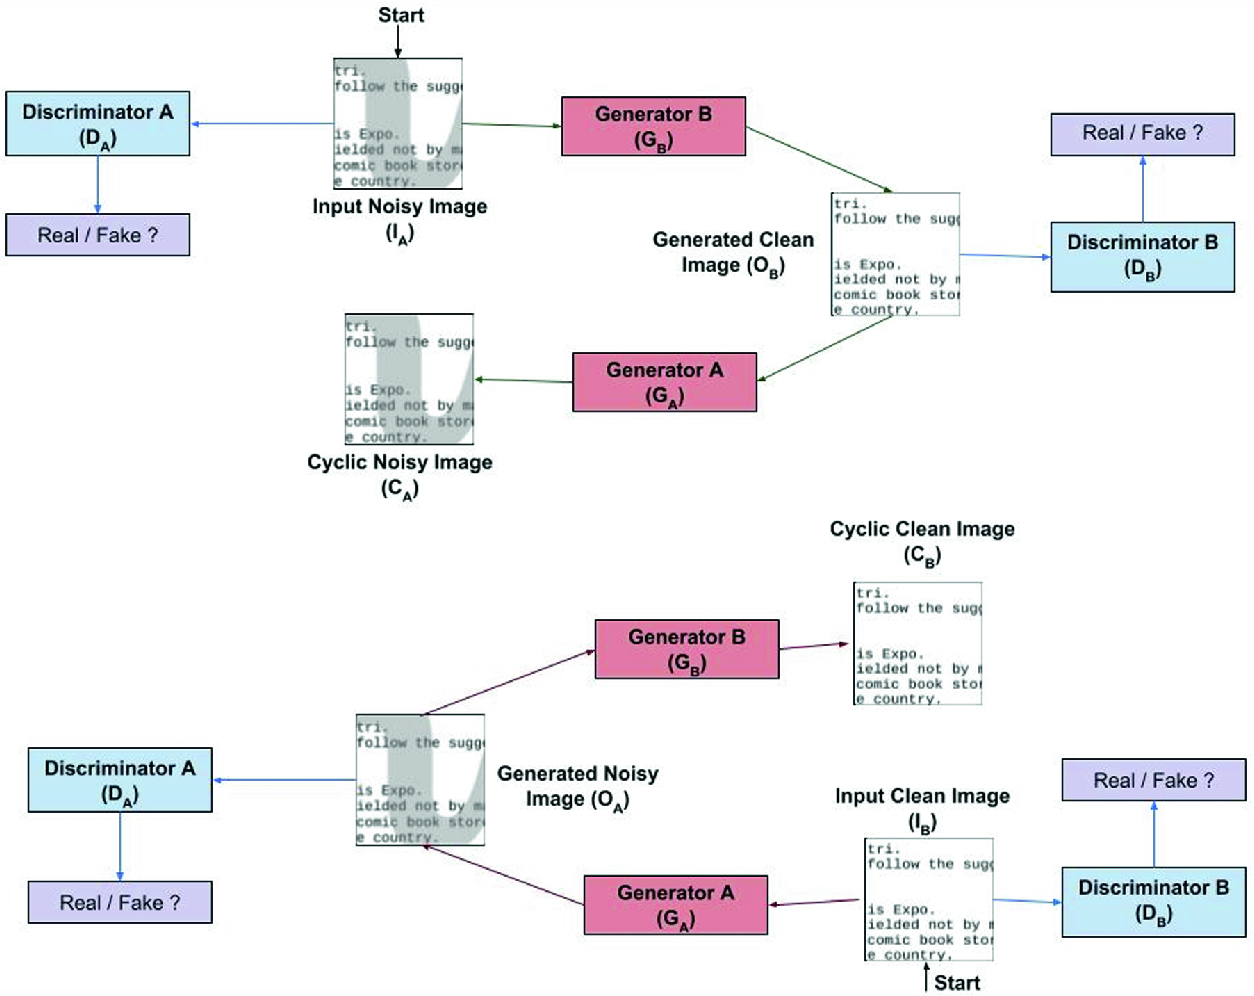
\includegraphics[scale=1.20]{images/relatedWorks/LearningToClean.jpg}
	    \caption[An illustration of \ac{CycleGAN} transforming the noisy images into clean images and vice versa.]{An illustration of \ac{CycleGAN} -  It has two generators $G_A$ and $G_B$ and two discriminators $D_A$ and $D_B$. The generator $G_A$ transforms the noisy images into clean images and $G_B$ transforms clean images into noisy images using cycle-consistency loss \cite{zhu2020unpaired}. The discriminators $D_A$ and $D_B$ rejects samples generated by $G_A$ and $G_B$ respectively acting as an adversary \cite{sharma2019learning}.}
	    \label{fig:LearningToClean}
	    \end{center}
\end{figure}



Monika Sharma et al.\ \cite{sharma2019learning} are addressing a problem in the scanning process that often results in the introduction of blur due to camera motion, salt and pepper noise, or water markings, shake, wrinkles, coffee stains, or faded data. These artifacts introduce several readability challenges in modern text recognition algorithms, decreasing their performance and accuracy \cite{sharma2019learning}. The current denoising techniques are based on a supervised learning approach using paired training datasets, in which it contains noisy documents with their corresponding cleaned versions of the same noisy document \cite{sharma2019learning}. However, in the real world, such a paired training dataset is not available to train a model, to generate clean documents from noisy versions \cite{zhu2020unpaired}\cite{sharma2019learning}. Hence, in this literature, the authors used \ac{CycleGAN} an unsupervised image-to-image translation technique to transform noisy document images into clean document images. \ac{CycleGAN} is a method to learn a mapping between two data distributions in the absence of paired training dataset \cite{zhu2020unpaired} \cite{sharma2019learning}. They have compared the performance of \ac{CycleGAN} for document cleaning tasks with \ac{cGAN} by training them over the same dataset. The only difference was \ac{CycleGAN} trained using unpaired images and \ac{cGAN} trained using the paired images. They have used \ac{PSNR}\footnote{Peak Signal-to-Noise Ratio: \url{http://www.ni.com/white-paper/13306/en/} last access: \dcdate.} as a evaluation metric to evaluate the quality of transformed denoised images. Experiments were performed on 4 separate public document datasets, one each for deblurring, watermark removal, background noise removal and defading. Finally, they concluded \ac{CycleGAN} learns a more robust mapping from the space of noisy to clean documents compared to \ac{cGAN} \cite{sharma2019learning}. The complete architecture of \ac{CycleGAN} for denoising documents illustrated in figure \ref{fig:LearningToClean}.


\begin{figure}[H]
        \begin{center}
 	    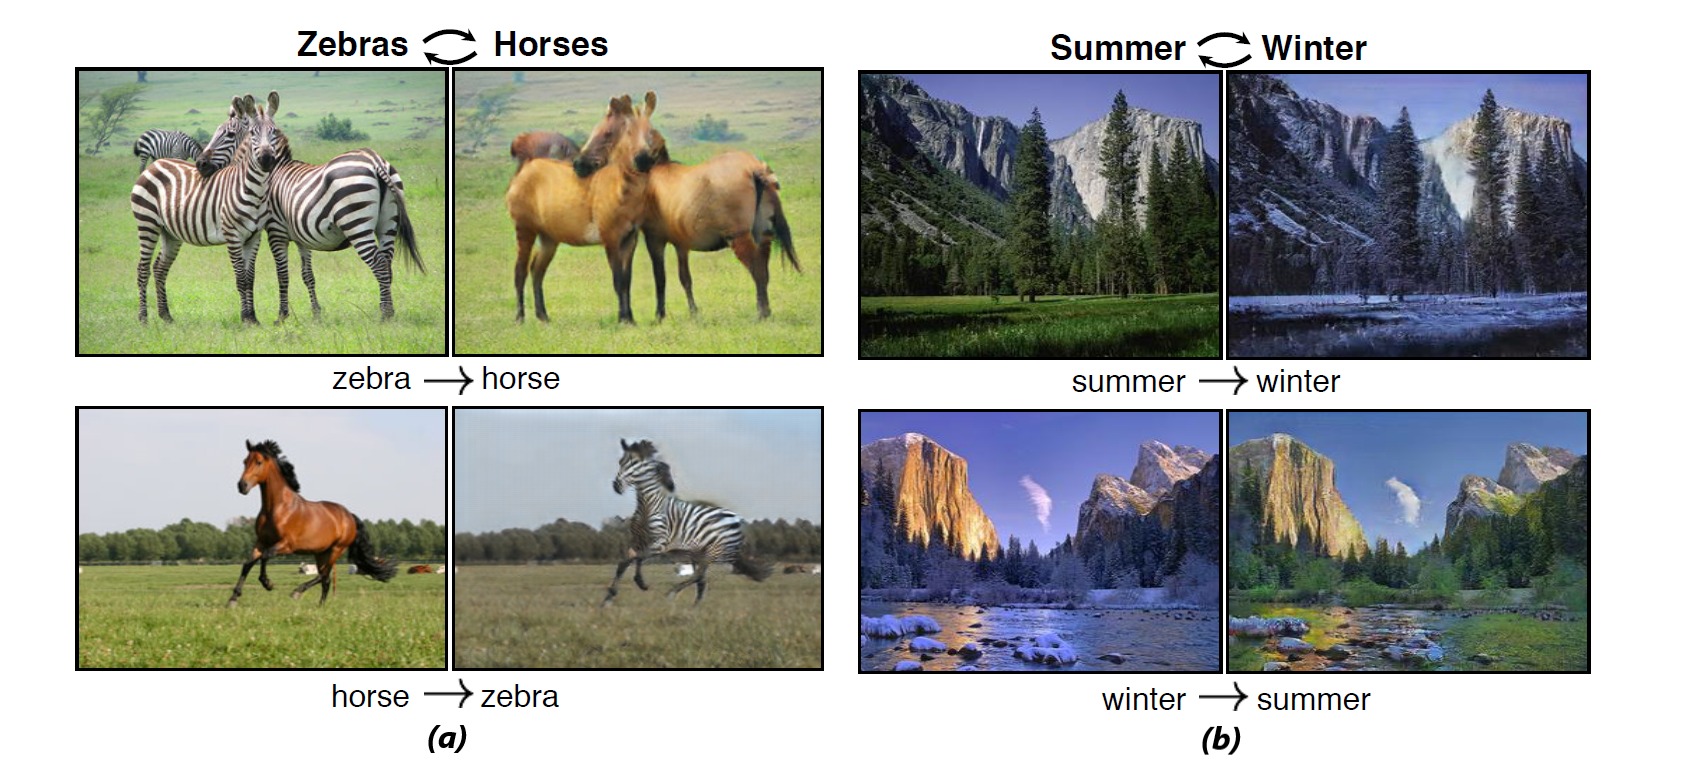
\includegraphics[scale=0.35]{images/relatedWorks/CycleGANExamples.png}
	    \caption[An illustration of \ac{CycleGAN} transforming an image from one into the other and vice versa.]{An illustration of \ac{CycleGAN} transforming an image from one into the other and vice versa. For example, (a) zebra image transformed into horse image and vice versa and (b) the view of Yosemite mountains in summer transformed into winter and vice versa \cite{zhu2020unpaired}.}
	    \label{fig:CycleganExamples}
	    \end{center}
\end{figure}


Jun-Yan Zhu et al.\ \cite{zhu2020unpaired} noticed the scarcity of paired training data to perform image-to-image translation. Hence, they proposed \ac{CycleGAN} as an image-to-image translation method that can transform the images from source domain $X$ to target domain $Y$ in the absence of paired training dataset. This method learns to capture underlying characteristics of the collection of images in the source domain and figuring out how these characteristics could be transformed into the collection of images in the target domain, all in the absence of any paired training examples \cite{zhu2020unpaired}. In this method, the goal is to learn a mapping $G\ \colon X \rightarrow Y$ so that the generated distribution of images $G(X)$ matches the target distribution $Y$ using an adversarial loss. However, the adversarial losses alone are not sufficient to map the images from the source domain to the target domain. Hence, authors introduced inverse mapping $F\ \colon Y \rightarrow X$ to introduce a cycle-consistency loss to enforce $F(G(X))\approx X$ and vice versa to regularize the output and keep it highly under-constrained \cite{zhu2020unpaired}. The cycle-consistency property of an image-to-image translation can be understood by a simple example, if we translate a sentence of English to French, again back from French to English, one should arrive back to the original sentence. In this manner, \ac{CycleGAN} learns to produce images within the context instead of generating random images\footnotemark. Authors investigated several prior methods like Bi-GAN/ALI \cite{donahue2017adversarial} \cite{dumoulin2017adversarially}, CoGAN \cite{liu2016coupled}, SimGAN \cite{shrivastava2017learning} were unable to achieve compelling results. However, \ac{CycleGAN} often produces images that are equivalent quality to the fully supervised pix2pix software \cite{isola2018imagetoimage}. Authors provided \href{https://github.com/junyanz/pytorch-CycleGAN-and-pix2pix}{PyTorch} implementation of \ac{CycleGAN}. The figure \ref{fig:CycleganExamples} illustrates, examples of \ac{CycleGAN} transforming an image from one into the other and vice versa.

\footnotetext{\url{https://machinelearningmastery.com/what-is-cyclegan/} last access: \dcdate}

Chris Tensmeyer et al.\ \cite{8978087} realized solving binarization tasks using deep learning models is very challenging. It is due to the scarcity of large quantities of labeled data available to train such models. There have been efforts to create synthetic data for binarization using image processing techniques but, they generally lack realism \cite{8978087}. Hence, authors proposed DGT-CycleGAN to produce realistic synthetic data using an adversarially trained image-to-image translation model \cite{8978087}. Authors modified the \ac{CycleGAN} model to be conditioned on the ground truth binarization mask as it transforms images from the source domain of synthetic images to the target domain of real images \cite{8978087}. They found modifying the discriminator to condition on the binarization \ac{GT} leads to increased realism and better agreement between the \ac{GT} and the produced image \cite{8978087}.  Authors pretrained deep learning models on realistic synthetic datasets generated by \ac{CycleGAN}, DGT-CycleGAN and image compositing \cite{8978087}. They found pretraining a model on realistic synthetic data generated by the DGT-CycleGAN model achieves the best performance for solving binarization tasks compared to data generated by \ac{CycleGAN} and image compositing \cite{8978087}. Also, they evaluated both pretrained only and finetuned models on each of the \ac{DIBCO} datasets\footnotemark to measure their performance \cite{8978087}. Finetuning a model on \ac{DIBCO} dataset after pretraining on the realistic synthetic images generated by the DGT-CycleGAN has lead to a 13\% reduction of F-measure error compared to no pretraining and to 6\% error reduction compared to pretraining on non-realistic synthetic data \cite{8978087}. Authors concluded, pretraining deep neural networks on the realistic synthetic data generated using DGT-CycleGAN lead to better predictive performance both before and after finetuning on real data.

\footnotetext{\ac{DIBCO} 2019: \url{https://vc.ee.duth.gr/dibco2019/} last access: \dcdate}


\section{Summary}\label{rwsummary}
Over the years, \acp{GAN} have evolved to solve different kinds of problems (figure \ref{fig:GANEvolution}). General \acp{GAN} suffer from unstable training, vanishing gradients problem and mode collapse. Therefore, Martin Arjovsky et al.\ \cite{arjovsky2017wasserstein} proposed \acp{WGAN} to solve problems with \acp{GAN}. \acp{WGAN} solve problems like mode collapse, improve learning stability and provide meaningful learning curves beneficial for hyperparameter searches and debugging \cite{arjovsky2017wasserstein}. Although the implementation of \ac{WGAN} is straightforward, the theory behind it is difficult and requires modifications, for example, implementation of Weight Clipping \cite{gulrajani2017improved}. Hence, Xudong Mao et al.\ \cite{mao2017squares} proposed a simple and more intuitive method compared to \ac{WGAN}, called \ac{LSGAN}. First, \acp{LSGAN} generate higher quality images than \acp{GAN} \cite{mao2017squares}. Second, its learning process is stable compared to \acp{GAN} \cite{mao2017squares}. Monika Sharma et al.\ \cite{sharma2019learning} demonstrated \ac{CycleGAN} can transform noisy document images into denoised and clean document images. They demonstrated \ac{CycleGAN} transforms noisy document images into clean document images superior to \ac{cGAN}. Chris Tensmeyer et al.\ \cite{8978087} proposed DGT-CycleGAN, a modified version of \ac{CycleGAN}, which is adequate to translate images from the domain of synthetic images to the domain of real images to solve binarization tasks. Taesung Park et al.\ \cite{park2020contrastive} proposed \ac{CUT}. They have demonstrated that \ac{CUT} is a better, faster and memory-efficient approach to perform unsupervised image-to-image translation. Further, Jun-Yan Zhu et al.\ \cite{zhu2020unpaired} proposed an unsupervised image-to-image translation approach \ac{CycleGAN} to address the problem of scarcity of paired training data while training image-to-image translation applications. Compared to \acp{GAN}, \acp{CycleGAN} also can deal more meticulously with the problems like unstable training, vanishing gradients problems and mode collapse. In this thesis, the image-to-image translation model is developed using \ac{LSGAN} and \ac{CycleGAN}. The generators and discriminators are optimized using cycle-consistency loss \cite{zhu2020unpaired} and least-square loss \cite{mao2017squares}. The proposed method is simple and capable to solve problems in general \acp{GAN}. Also, it learns a function of image-to-image translation in the absence of paired training data using cycle-consistency property \cite{zhu2020unpaired}.



\begin{comment}
\section{Conclusion}\label{rwconclusion}

The image-to-image translation is a classic example of computer vision and computer graphics problems. In which the goal is to learn the mapping between a source image and target image using a training set of aligned image pairs. Although, for many tasks, aligned or paired training data will not be available. Also, collecting and annotating paired document images is tedious, difficult, time-consuming and costly. This thesis is attempting to close a domain gap between synthetic document images and real document images in the absence of paired training data. The thesis proposes an image-to-image translation application to transform synthetic document images into realistic document images to perform domain adaptation, by closing the gap between synthetic data distribution and real data distribution. Ultimately, a large amount of realistic annotated set of document images can be generated using this application. Furthermore, they can be used to improve real document image classification. Also, in case, if a classifier is trained using such generated realistic document images, it can fasten the process of labeling the new annotated or unlabeled real document images. As per the above literature survey \cite{zhu2020unpaired} \cite{sharma2019learning} and problem statement, in this thesis \ac{CycleGAN} is a decided method to transform synthetic document images into realistic document images in the absence of paired training data. Hence, the proposed image-to-image translation application is realized using \ac{CycleGAN}.
\end{comment}





























%Authors considered evaluation metrics like \ac{AMT} perceptual studies, FCN-score \cite{isola2018imagetoimage} and semantic segmentation metrics to compare the quality of generated images against other baseline. 
%The evaluation metrics like \ac{FID} \cite{heusel2018gans} and semantic segmentation scores are used to compare the quality of generated images using \ac{CUT} method. 

%Authors performed multiple experiments during ablation studies using evaluation metrics like, \ac{AMT} perceptual study, FCN-Score and semantic segmentation metrics. 

%In this thesis, \ac{CycleGAN} is used to perform domain adaptation. Discussion about the loss functions has been carried out in-depth in Chapter \ref{methodology}.
%is combined with \ac{LSGAN}, in which the discriminator model is updated using a least-squares loss (L2 Loss).
%The thesis aims to develop an image-to-image translation application to transform synthetic document images into realistic document images. The thesis aims to develop an image-to-image translation application to transform synthetic document images into realistic document images to perform domain adaptation. Ultimately, a large amount of realistic annotated set of document images can be generated using this application.





\newpage    


\chapter{Fundamentals}
    \label{fundamentals}
    %\noindent
\justifying
\setlength{\parskip}{1em}

This chapter focuses on improving the understanding of the fundamental concepts required to understand this thesis. Section \ref{GenerativeAdversarialNetworks} describes architecture of \acp{GAN}. Section \ref{CNNs} describes neural network layers, namely, convolution layer, activation layer, pooling layer and fully connected layer.


\section{Generative Adversarial Networks (GANs)}\label{GenerativeAdversarialNetworks}

\begin{figure}[H]
        \begin{center}
	    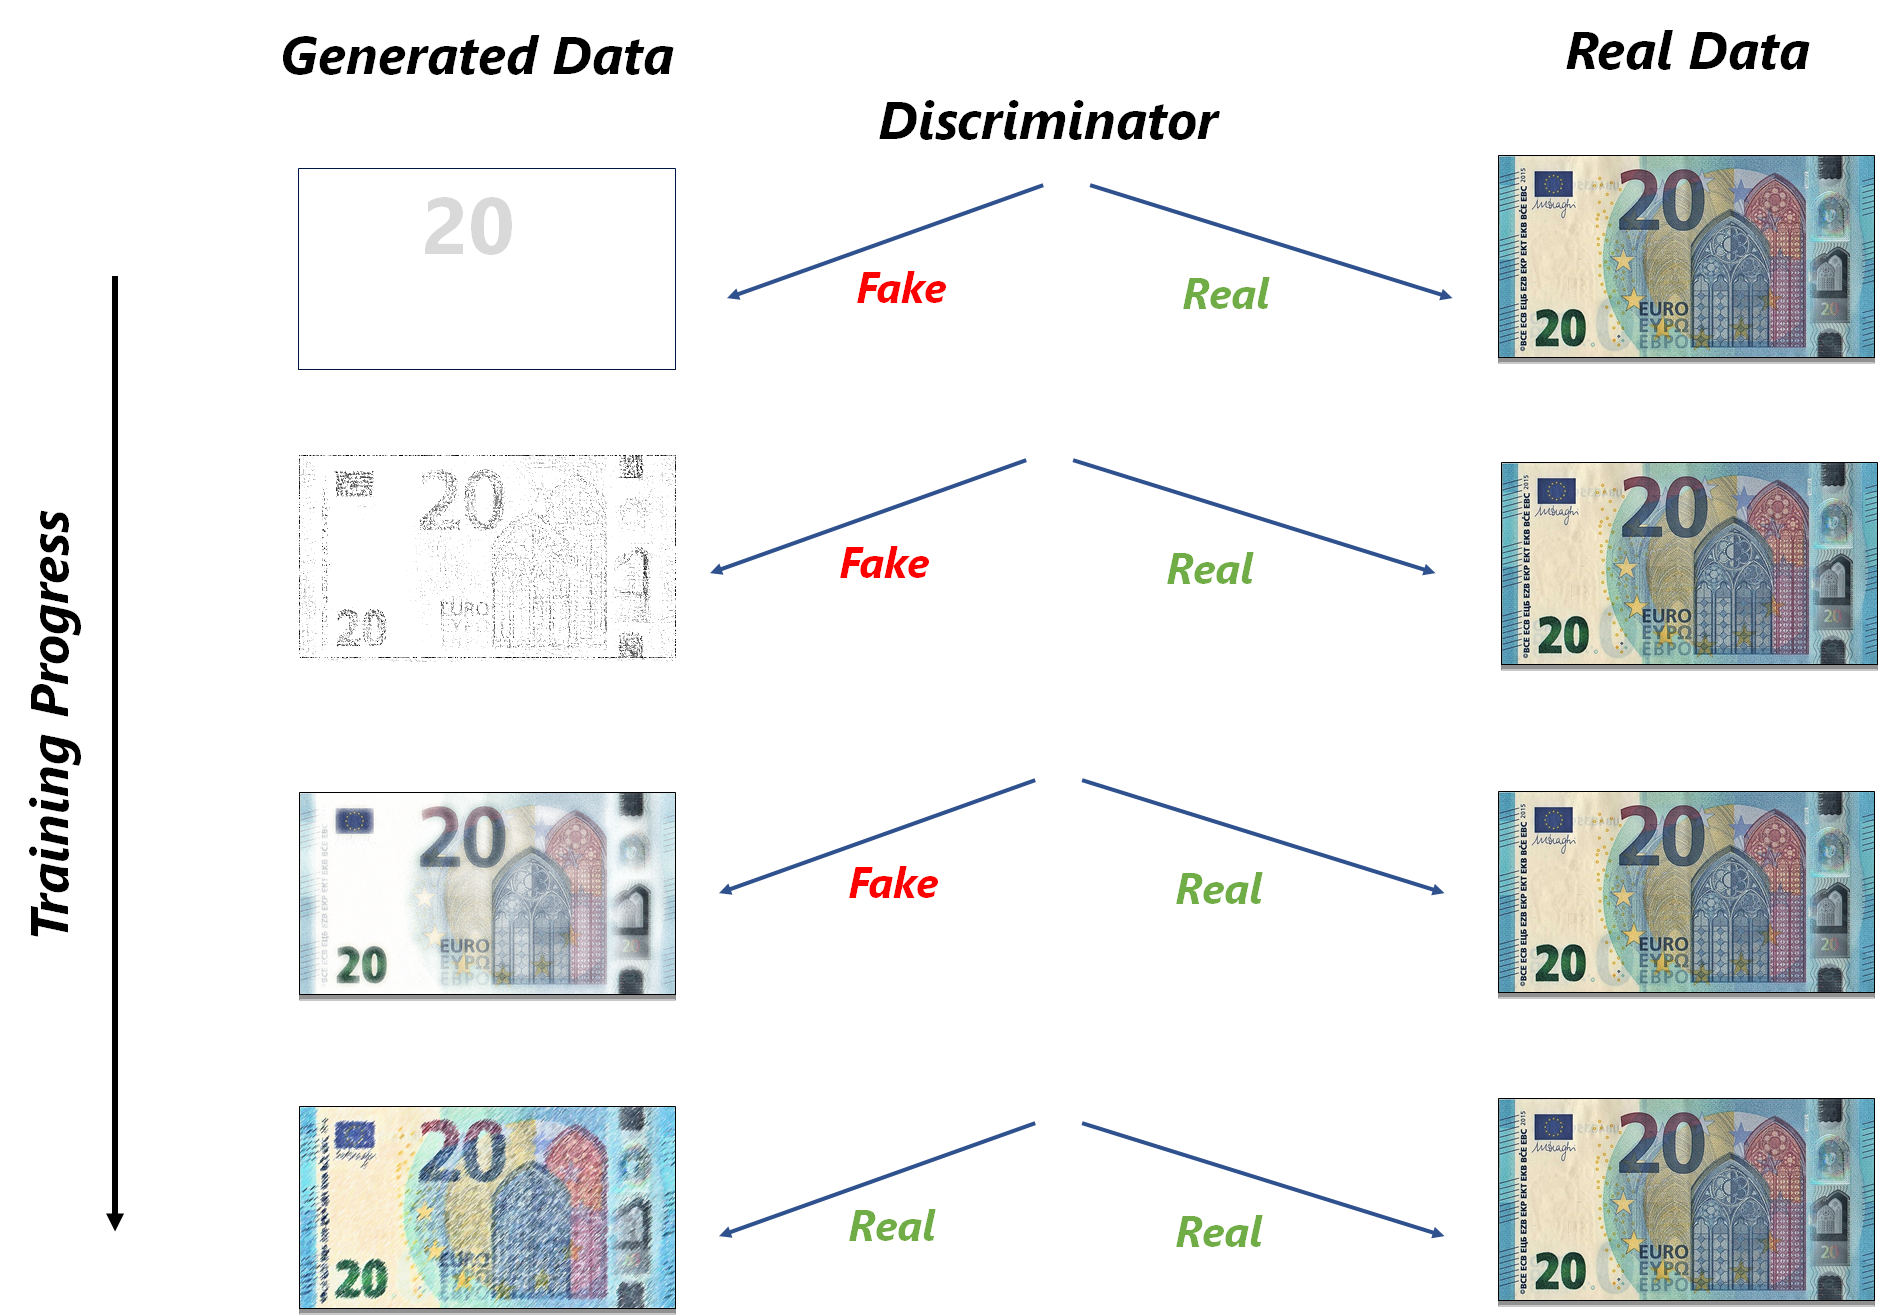
\includegraphics[scale=0.30]{images/Fundamentals/GANTrainingintuition.png}
	    \caption[Intuitive example of \ac{GAN} training progress.]{Intuitive example of \ac{GAN} training progress.}
	    \label{fig:GANTrainingintuition}
	    \end{center}
\end{figure}

% Both generator and discriminator are trained simultaneously. 
%, the multilayer perceptron can loosely be indicated by \acp{ANN}

\acp{GAN} have two models in their architecture first is the generator and the second is the discriminator and both models can be implemented using multilayer perceptrons \cite{goodfellow2014generative}. Let's try to understand the function of \acp{GAN} intuitively. Consider generator is a forger who creates fake currencies, with the intention of making them realistic as much as possible. Further, the discriminator is an expert who distinguishes forged and real currencies. The discriminator has access to images generated by the generator and real images present in the dataset. The generator generates fake images without having access to the real images using random noise distribution. The discriminator learns by the feedback error after misclassifying real images as fake and fake images as real. The generator also learns by the feedback error given by the discriminator, after it successfully classifies image produced by the generator as fake. To produce a better quality of fake images, the generator model is updated using the feedback error given by the discriminator. It is a setup where both generator and discriminator are competing with each other. An intuitive example of \ac{GAN} training process is illustrated in figure \ref{fig:GANTrainingintuition}. It depicts, during the initial stages of the training, the generated images by the generator are easily distinguished as fake by the discriminator. After training iterations, the quality of the generated images by the generator increases. The generator learns using feedback error given by the discriminator. Finally, the generator learns to produce realistic images and the discriminator starts to classify them as real.

Now, let's have a look into the \ac{GAN}'s architecture. As described earlier, the task of the \ac{GAN} is to generate fake samples that are realistic. The training dataset of real data samples $S$ serves as an input to the discriminator $D$. The random noise vector $Z$ retrieved from the random noise distribution serves as an input to the generator $G$ to produce fake samples. The generator $G$ takes $Z$ as an input and outputs a fake sample $S'$. Its goal is to create fake samples that are realistic as much as possible and indistinguishable from the real samples from the training dataset. The discriminator $D$ takes input from real data sample $S$ that are present in the training dataset and fake samples $S'$ generated from the generator $G$. For each sample, it determines and outputs the probability of the sample that is real. For every discriminator's prediction, the classification error is backpropagated to update both generator and discriminator during iterative training. The discriminator's weights are updated to maximize classification accuracy which means, maximizing the probability of correct prediction $S$ as real and $S'$ as fake. The generator's weights are updated to produce quality samples and maximize the probability that the discriminator makes mistake and misclassifies $S'$ as real. \ac{GAN} in action is illustrated in figure \ref{fig:GANStructure}.


%The training dataset has a set of real data samples, from which the generator learns to create fake samples that are similar to the real samples
%Also, the discriminator gets smarter and smarter over time, to distinguish fake images and real images, like mentioned earlier both models are trained simultaneously. But at a certain point generator starts to produce realistic images which the discriminator classifies as real. 
%The discriminator learns by the error signal provided by the ground truth of distinguishing whether the image came from the dataset of real images or from the generator. The generator learns using the same error signal given by the discriminator to produce a better quality of forged or fake images. It is a setup where both generator and discriminator are competing with each other.


%\vspace*{0.1cm}
\begin{figure}[H]
        \begin{center}
	    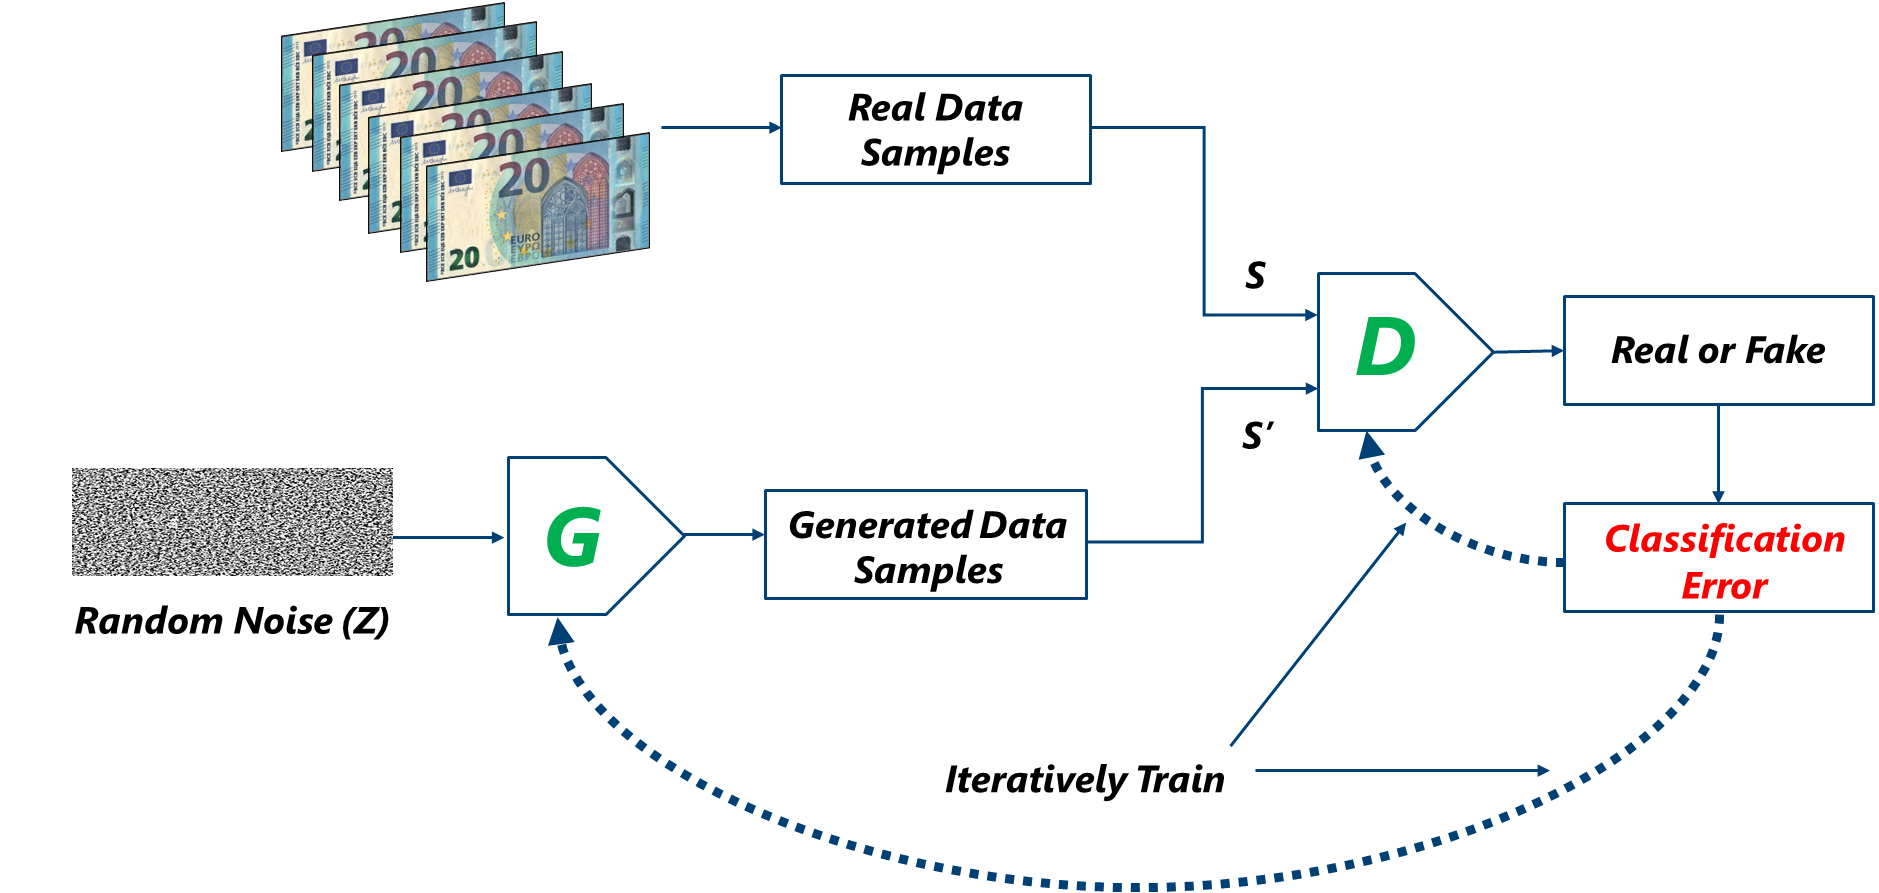
\includegraphics[scale=0.30]{images/Fundamentals/GANStructure.png}
	    \caption[An illustration of \ac{GAN} architecture.]{An illustration of \ac{GAN} architecture along with the generator's and discriminator's inputs, outputs and their interactions.}
	    \label{fig:GANStructure}
	    \end{center}
\end{figure}


%In practice, the discriminator is may not be trained till it is optimal \cite{Creswell_2018}.

Let's try to understand the mathematics behind \acp{GAN}. For learning the generator’s distribution $p_g$ over data $x$, the input noise variable defined as $p_z(z)$. The generator $G$ and discriminator $D$ are the differential functions. They are represented by multilayer perceptrons with parameters $\theta_g$ and $\theta_d$ respectively \cite{goodfellow2014generative}. The mapping function from some representation space, called, the latent space to the space of data, is represented by $G(z; \theta_g)$. The $D(x; \theta_d)$ maps data $x$ to the probability that it came from the real data distribution rather than generator distribution $p_g$. Basically, $D(x)$ represents the likelihood of $x$ came from the data rather than $p_g$. $D(x; \theta_d)$ outputs a single scalar value between $[0,1]$. $D$ is trained to maximize the probability of correctly labeling both training examples and data generated by the $G$. Usually, when the generator is training, the discriminator does not train and vice versa. For a fixed $G$, the discriminator is trained to classify data as either being from the real data distribution (real, probability close to one) or from the fixed generator(fake, probability close to zero). After a certain number of training iterations, when the discriminator is optimally optimized, it can be fixed and the generator $G$ advances to learn by the error provided by the discriminator to produce plausible data. At the end of the training, if the generator can match the real data distribution, then the discriminator is maximally confused, will predict 0.5 probability for its inputs and mathematically $G$ is being trained to minimize $log(1 - D(G(z))$. It can be said $D$ and $G$ compete with each other just like a two-player minimax game to achieve the objective $\mathcal{L}_{GAN}(G, D)$:


\begin{equation}\label{ganObjectiveFunction}
\underset{G}{\min}\ \underset{D}{\max}\ \mathcal{L}_{GAN}(D, G) = E_{x\sim p_{data}(x)}[log D(x)] + E_{z\sim p_z(z)}[log(1 - D(G(z)))].
\end{equation}


Authors mentioned, in practice, the equation \ref{ganObjectiveFunction} may not give enough gradient for $G$ to learn well. During early in learning phase, when $G$ is poor, $D$ can reject samples with high confidence because they are clearly distinct from the training data. In this case, term $log(1 - D(G(z)))$ in equation \ref{ganObjectiveFunction} saturates very quickly \cite{goodfellow2014generative}. Hence, Authors proposed to train $G$ to maximize $log D(G(z))$ rather than training it to minimize $log(1 - D(G(z)))$. This modified objective function leads to the same fixed point of the dynamics of $G$ and $D$ by providing much stronger gradients early in learning \cite{goodfellow2014generative}. The \ac{GAN} converging to match generated data distribution $p_g$ to real data distribution $p_{data}$ is illustrated in the figure \ref{fig:GANTraining}.

\begin{figure}[H]
        \begin{center}
	    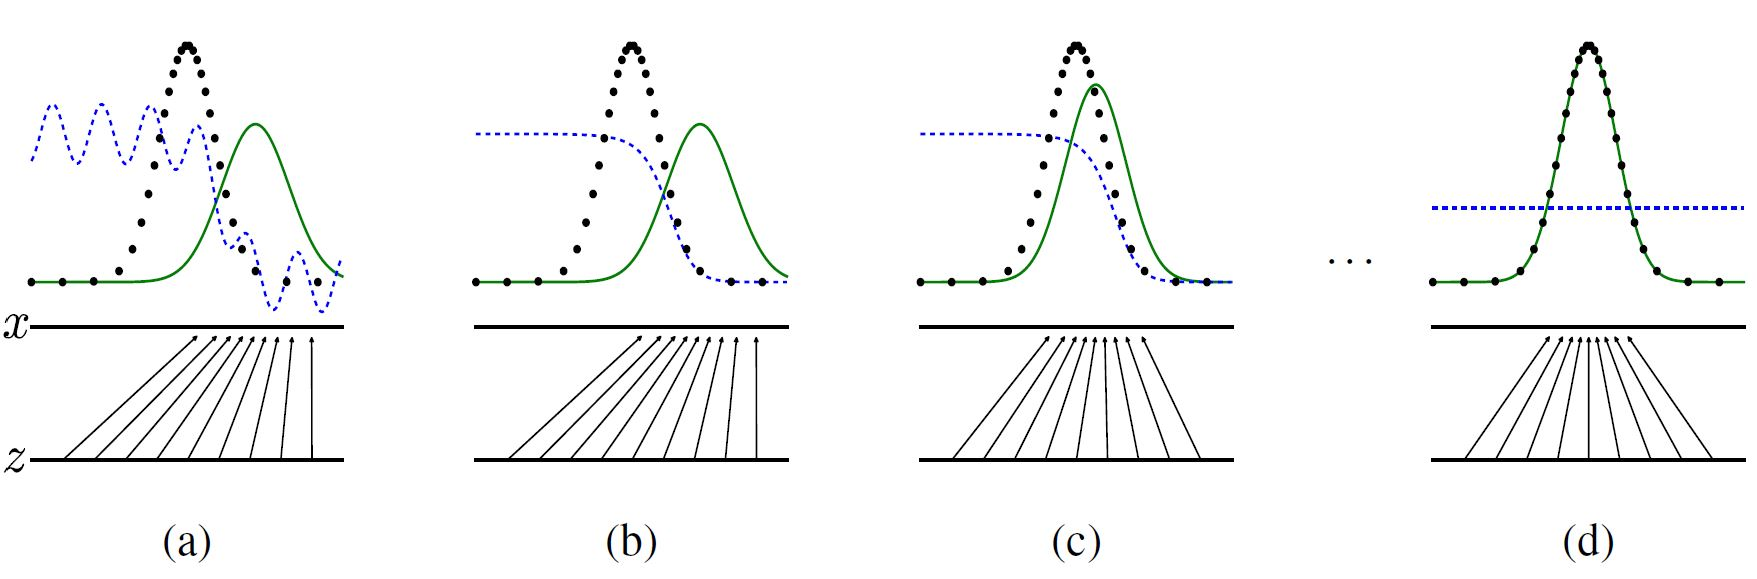
\includegraphics[scale=0.49]{images/Fundamentals/GANTraining.jpg}
	    \caption[An illustration of \ac{GAN} converging to match generated data distribution $p_g$ to real data distribution $p_{data}$.]{An illustration of \ac{GAN} converging to match generated data distribution $p_g$ to real data distribution $p_{data}$. While training \acp{GAN}, discriminative distribution is simultaneously updated so it will discriminate or distinguish samples from the real data distribution $p_x$ from those of the generated data distribution $p_g$. In the figure, the discriminative distribution is represented by ($D$, dashed line, blue), the real data distribution $p_x$ represented by (dotted line, black) and the generated data distribution $p_g$ represented by (G, green, solid line).
	    
	    
	    
	    
	    
	    
	    
	    The lower horizontal line represents the domain of noise distribution $p_z$ from which $z$ is sampled uniformly. The horizontal line above represents the part of the domain of real data $x$. The upward arrows depict the mapping of $x = G(z)$, which creates the non-uniform generated data distribution $p_g$ on transformed samples. (a) Consider, $G$ and $D$ are on the verge of convergence, $p_g$ is almost similar to $p_{data}$ and $D$ is a partially accurate classifier. (b) Slowly, $D$ is trained further to distinguish real data samples from generated data samples. For a fixed $G$, there is an optimal discriminator, $D^*(x) = \frac{p_{data}(x)}{p_{data}(x) + p_g(x)}$. (c) The $G$ is updated using gradients that are backpropagated from $D$ and makes $G(z)$ to flow into the regions that are most probably classified as real data, the parameters of the $G$ are updated, while the parameters of the $D$ are fixed. (d) After several steps of training, $G$ is optimal where $p_g = p_{data}$, which is equivalent to the optimal $D$ predicting 0.5 for all samples drawn from $x$, at this stage $D$ is maximally confused and will not able to distinguish real data samples from generated data samples, i.e. $D(x) = \frac{1}{2}$ \cite{goodfellow2014generative}.}
	    \label{fig:GANTraining}
	    \end{center}
\end{figure}

\subsection{\ac{GAN} Training}

% In figure \ref{fig:generatorAndDiscriminatorTraining} shows the same \ac{GAN} network in different stages of the training process at distinct time points.

This section discusses the training algorithm of the \ac{GAN}. The training algorithm is divided into two sections. These two sections are discriminator training and generator training. It illustrates the discriminator and generator training process together. It also illustrates, while training the generator, the discriminator is not training, basically, it means, a fixed discriminator is used while training the generator. Hence, the training dataset of real data samples is grayed out in the section where the generator training is illustrated, and while training discriminator both generated samples from the generator and real samples are used as an input. In the following sections generator's and discriminator's training process is described along with intuitive figures. Further, the \ac{GAN} training algorithm has been described in the form of pseudo-code. The algorithm of the \ac{GAN} is pictorially illustrated in the figure \ref{fig:generatorAndDiscriminatorTraining}

\subsubsection{Discriminator Training}\label{TheDiscriminatorSubSection}

In \acp{GAN}, the discriminator is a binary classifier. It attempts to classify real data samples from fake data samples generated by the generator. It provides the likelihood that its input is a real data sample. In computer vision tasks, the discriminator classifies images, hence, it is implemented using \ac{CNN} \cite{radford2016unsupervised}. The discriminator's training data come from the two resources, training dataset or collection of real data samples and fake data samples generated by the generator. The discriminator is penalized for misclassifying a real data sample as fake or a fake data sample as real, such classification error is called discriminator loss. The weights of the discriminator network are updated using backpropagated discriminator loss. The training process of the discriminator $D$ using backpropagation illustrated in figure \ref{fig:discriminatorTraining}.

%The discriminator can be implemented using a multilayer perceptron which is suitable to the kind of data it's classifying. 
%During \ac{GAN} training, the discriminator is trained by both real data samples and fake data samples generated by the generator.

%\vspace*{0.2cm}
\begin{figure}[H]
        \begin{center}
	    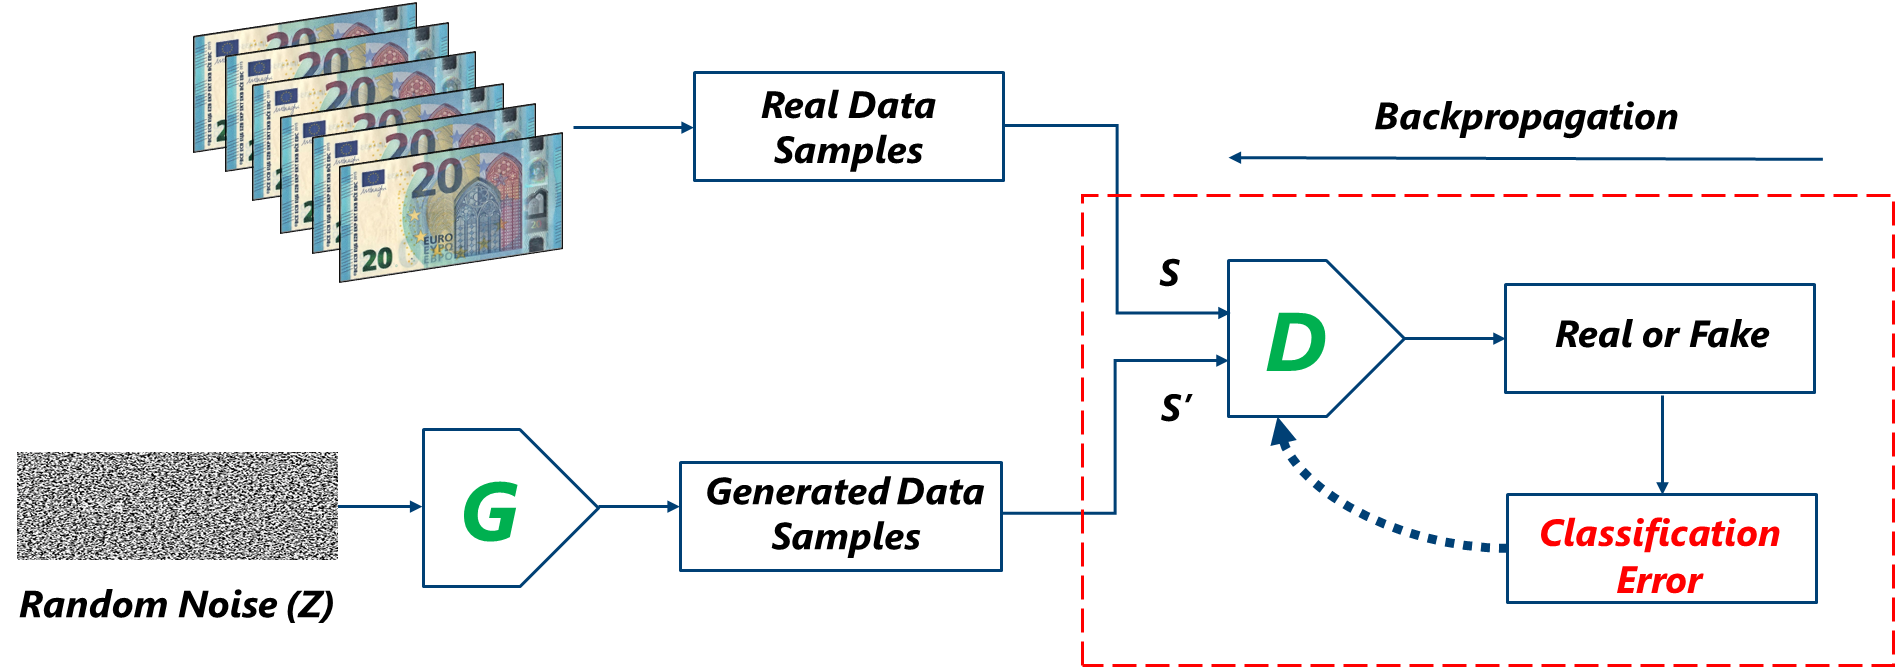
\includegraphics[scale=0.30]{images/Fundamentals/discriminatorTraining.png}
	    \caption[An illustration of the training of the discriminator $D$ using backpropagation.]{An illustration of the training of the discriminator $D$ using backpropagation.}
	    \label{fig:discriminatorTraining}
	    \end{center}
\end{figure}

\subsubsection{Generator Training}\label{TheGeneratorSubSection}

The generator produces fake samples using random noise vectors sampled from the random noise distribution. In computer vision tasks, the generator usually produces fake images, hence, it is implemented using \ac{CNN} \cite{radford2016unsupervised}. The generator aims to produce fake samples that are as realistic as possible, but if the generator fails to fool the discriminator, in other words, if the discriminator recognizes and classifies the generated samples as fake, then it is penalized with classification error, such classification error is called generator loss. The weights of the generator are updated using backpropagated generator loss. The training process of the generator $G$ using backpropagation is illustrated in figure \ref{fig:generatorTraining}.

%The generator's task is to generate images using the random noise distribution, so it is implemented using \ac{CNN} \cite{radford2016unsupervised}.
%As described earlier, the discriminator's weights are frozen while training the generator. This means the discriminator is not training while the generator is generating fake samples and vice versa. The generator can be implemented using a multilayer neural network which is suitable for the kind of data it's generating. 

%\vspace*{0.2cm}
\begin{figure}[H]
    \begin{center}
	\includegraphics[scale=0.47]{images/Fundamentals/generatorTraining.png}
	\caption[An illustration of the training of the generator $G$ using backpropagation.]{An illustration of the training of the generator $G$ using backpropagation.}
	\label{fig:generatorTraining}
	\end{center}
\end{figure}




\subsubsection{\ac{GAN} Training Algorithm}

\begin{algorithm}[H]
\For{each training iteration}{
 \BlankLine
 \BlankLine
 \BlankLine
	\textbf{1. Train the Discriminator:}
	\BlankLine
	\BlankLine
		\Indp
		a) Get a real data sample $S$ from the training dataset. \\
		\BlankLine
		b) Get a noise vector $Z$ from the random noise distribution, pass it thorough the generator $G$ and create a fake sample $S'$. \\
		\BlankLine
		c) Classify $S$ and $S'$ using the discriminator $D$.\\
		\BlankLine
		d) Backpropagate the calculated classification error to update the discriminator’s weights to minimize classification error.\\
	\BlankLine
	\BlankLine
	\BlankLine
	\Indm
	\textbf{2. Train the Generator:}
	\BlankLine
	\BlankLine
		\Indp
		a) Get a noise vector $Z$ from the random noise distribution, pass it thorough the generator $G$ and create a fake sample $S'$. \\
		\BlankLine
		b) Classify $S'$ using the discriminator $D$.\\
		\BlankLine
		c) Backpropagate the calculated classification error to update the generator’s weights to maximize the discriminator’s error.\\
\BlankLine
\BlankLine
\BlankLine
}	
\caption{\ac{GAN} training algorithm \cite{langr2019gans}.}
\label{alg:ganTrainingAlg}
\end{algorithm}




\newpage
\section{Convolution Neural Networks}\label{CNNs}

In recent years deep learning is evolved with the rise of \acp{ANN}. \acp{ANN} are biologically inspired and capable to solve complex problems \cite{oshea2015introduction}. \acp{CNN} is the most successful image-driven pattern recognition technique among \acp{ANN} \cite{oshea2015introduction}. Nowadays, \acp{CNN} are used to solve difficult image recognition, image classification and object detection tasks. The \acp{CNN} have been a popular method because of its extraordinary results at object recognition competition known as the \ac{ILSVRC} in 2012 for solving computer vision tasks. \ac{CNN} is a kind of deep learning technique for processing data that has a grid pattern, for example, images and videos. \acp{CNN} are inspired by the early findings in the study of biological vision, especially, organization of the animal visual cortex \cite{Hubel.1968} \cite{Fukushima.1980} \cite{10.5555/3153997} and designed to automatically and adaptively learn spatial hierarchies of features, from low-level to high-level patterns \cite{10.5555/3153997}. It is composed of various building blocks, such as convolution layers, pooling layers and fully connected layers. As shown in figure \ref{fig:CNNBuildingBlocks}, the first two layers are convolution and pooling layers and they perform feature extraction. Whereas the third, a fully connected layer, maps the extracted and downsampled features from the convolution layers and pooling layers into the final output, such as probabilities for classification tasks \cite{articleCNNs}. Let's have a look at each layer in the following sections.

%In recent years in the field of machine learning, drastic improvements have occurred to increase the performance of machine learning models. Also, numerous deep learning techniques like \acp{ANN} are evolved significantly.
%These biologically inspired neural networks were able to exceed the performance compared to the traditional machine learning techniques to solve complex problems \cite{oshea2015introduction}. 


\vspace*{0.3cm}
\begin{figure}[H]
        \begin{center}
	    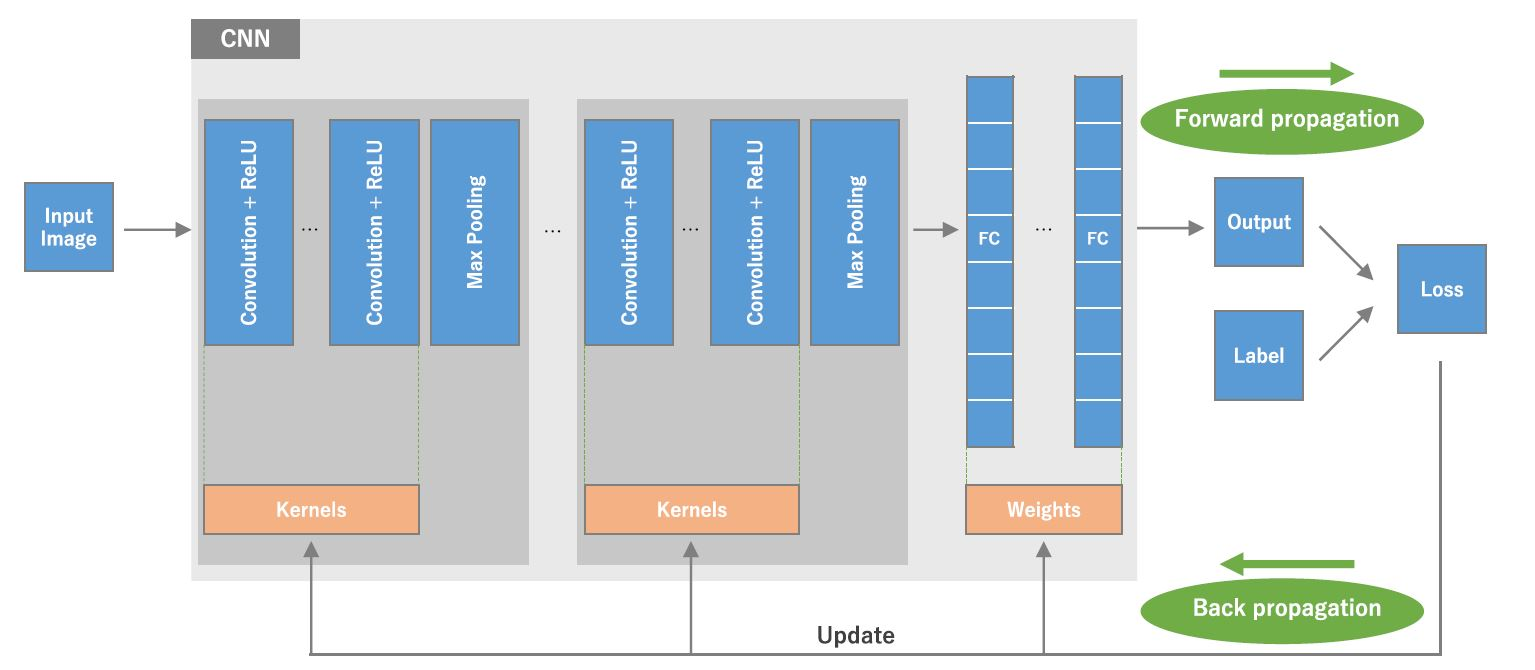
\includegraphics[scale=0.59]{images/Fundamentals/CNNBuildingBlocks.JPG}
	    \caption[An illustration of \ac{CNN} architecture and its training process.]{An illustration of \ac{CNN} architecture and its training process. Convolution layers, pooling layers and fully connected layers are the basic building blocks of \ac{CNN}. These layers are combined to build complex \ac{CNN} architectures to solve different types of problems. These building blocks are stacked upon each other. The \ac{CNN} is trained using the training dataset and the input data is fed into the network in a forward direction. The process of feeding data in the forward direction to the \ac{CNN} is called forward propagation. Each layer receives the input data and processes it through an activation function such as \ac{ReLU} (figure \ref{fig:ActivationFunctions}), then sends it on to the next successive layer. The model's performance is improved by updating the learnable parameters, weights and kernels using the loss value through backpropagation with gradient descent optimization algorithm \cite{ruder2017overview} \cite{articleCNNs}.}
	    \label{fig:CNNBuildingBlocks}
	    \end{center}
\end{figure}





\subsection{Convolution Layer}
The convolution layer is a basic component of the \ac{CNN} that performs feature extraction. It is typically a combination of linear and nonlinear operations like convolution operation and activation function \cite{articleCNNs}. It is one of the core building blocks of \acp{CNN}. Also, it computes for most heavy and complex computations. A convolution layer performs mathematical operations like convolution, a specialized type of linear operation \cite{articleCNNs}. The digital images store pixel values in a \ac{2D} grid, i.e., an array of numbers as shown in figure \ref{fig:Convolution}. The features from an image are extracted using a filter or kernel. A kernel is a small array of numbers applied across an input image, covering all pixels, using a given stride size. As features could exist at any location, the kernel is slid across an input, to perform an element-wise dot product between kernel elements and the input tensor, which is an array of pixel values. An element-wise dot product is performed between kernel's elements and an input tensor and results are added to obtain an output value at the corresponding location of the output tensor, such output tensor is called a feature map (figure \ref{fig:Convolution}a-c) \cite{articleCNNs}. This process extracts all vital features present in an image, making \ac{CNN} highly efficient for image processing and feature extraction tasks \cite{articleCNNs}.

%The layers are connected, one layer feeds its output to the next layer. ``The extracted features can hierarchically and progressively become more complex'' \cite{articleCNNs}. ``Training is the process of optimizing parameters such as kernels optimizing weights of the neurons in \acp{CNN}, which minimizes the difference between outputs and ground truth labels through an optimization algorithm backpropagation and gradient descent'' \cite{Goodfellow-et-al-2016} \cite{ruder2017overview} \cite{articleCNNs}.

\begin{figure}[H]
        \begin{center}
	    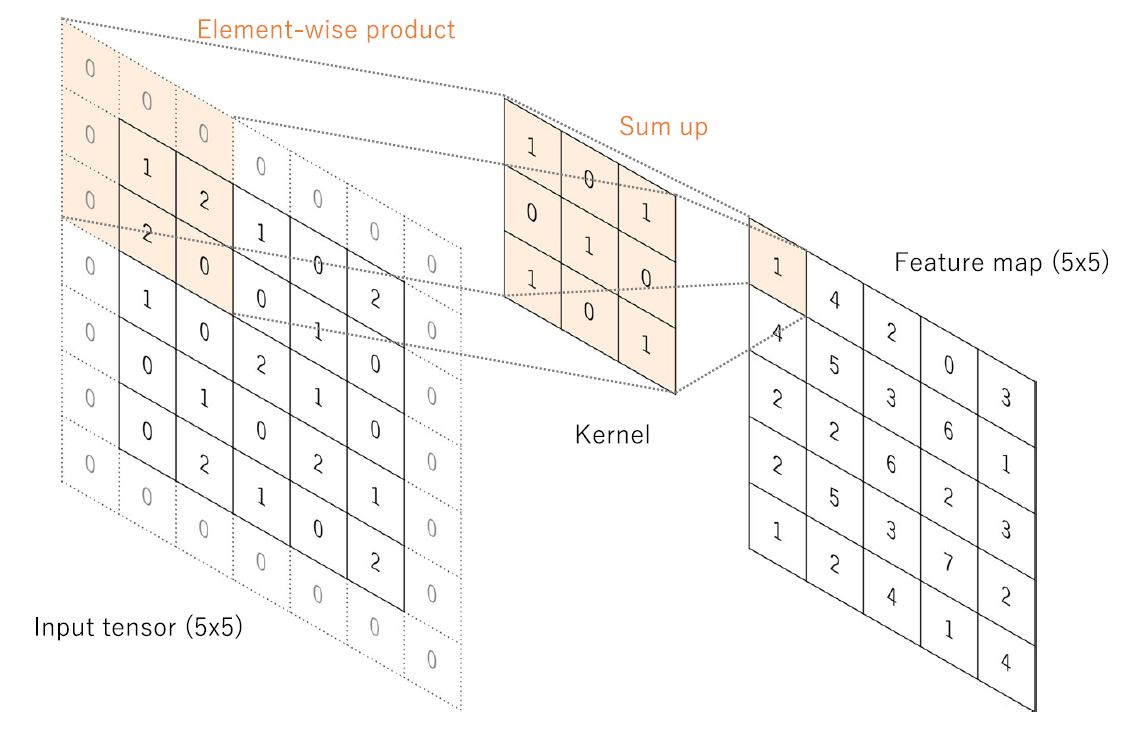
\includegraphics[scale=0.60]{images/Fundamentals/ConvolutionZeroPadding.JPG}
	    \caption[A Convolution Operation With Zero Padding.]{An illustration of a convolution operation with zero padding to retain spatial dimensions. Note that an input dimension of $5 \times 5$ is retained in the generated output feature map. In this example, kernel size is set to $3 \times 3$ and stride is set to $1$ \cite{articleCNNs}.}
	    \label{fig:ConvolutionZeroPadding}
	    \end{center}
\end{figure}

%``For feature extraction linear operation, convolution is used, where a small array of numbers, called a kernel, is applied across the input, which is an array of numbers, called a tensor. An element-wise product between the input tensor and kernel's each element is calculated at each location of the tensor and added to obtain the output value in the corresponding position of the output tensor, called a feature map (figure \ref{fig:Convolution}a-c)'' \cite{articleCNNs}. 

This procedure is repeated by applying multiple kernels to create an arbitrary number of feature maps, which describe different characteristics of the input tensors \cite{articleCNNs}. The different kernels act as separate feature extractors. Two important hyperparameters that represent the convolution operation are the size and number of kernels \cite{articleCNNs}. The size is typically 3 × 3, but sometimes 5 × 5 or 7 × 7, depends on the requirement. The number of kernels is arbitrary and determines the depth of output feature maps. The above-mentioned convolution operation prevents the center of each kernel from overlapping the input tensor's outermost element. Hence, the output feature map's height and width are reduced compared to the input tensor \cite{articleCNNs}. This problem is solved by the zero-padding. In this technique, extra rows and columns of zeros are added around the input tensor so that the kernel's center element overlaps with an outermost element of an input tensor. Zero padding helps to preserve the original spatial dimension throughout convolution operation (figure \ref{fig:ConvolutionZeroPadding}) \cite{articleCNNs}. Modern \ac{CNN} architectures normally employ zero padding to retain spatial dimensions to apply more further layers. Each successive feature map would get smaller after the successive convolution operation without zero padding. A stride is the distance between two successive kernel positions and it also defines the convolution operation \cite{articleCNNs}. A stride of 1 is the most common choice; however, a stride greater than 1 is sometimes used to achieve feature map downsampling. A pooling operation is an alternative technique for downsampling. It is described briefly in section \ref{PoolingLayer}.

\begin{figure}[H]
        \begin{center}
	    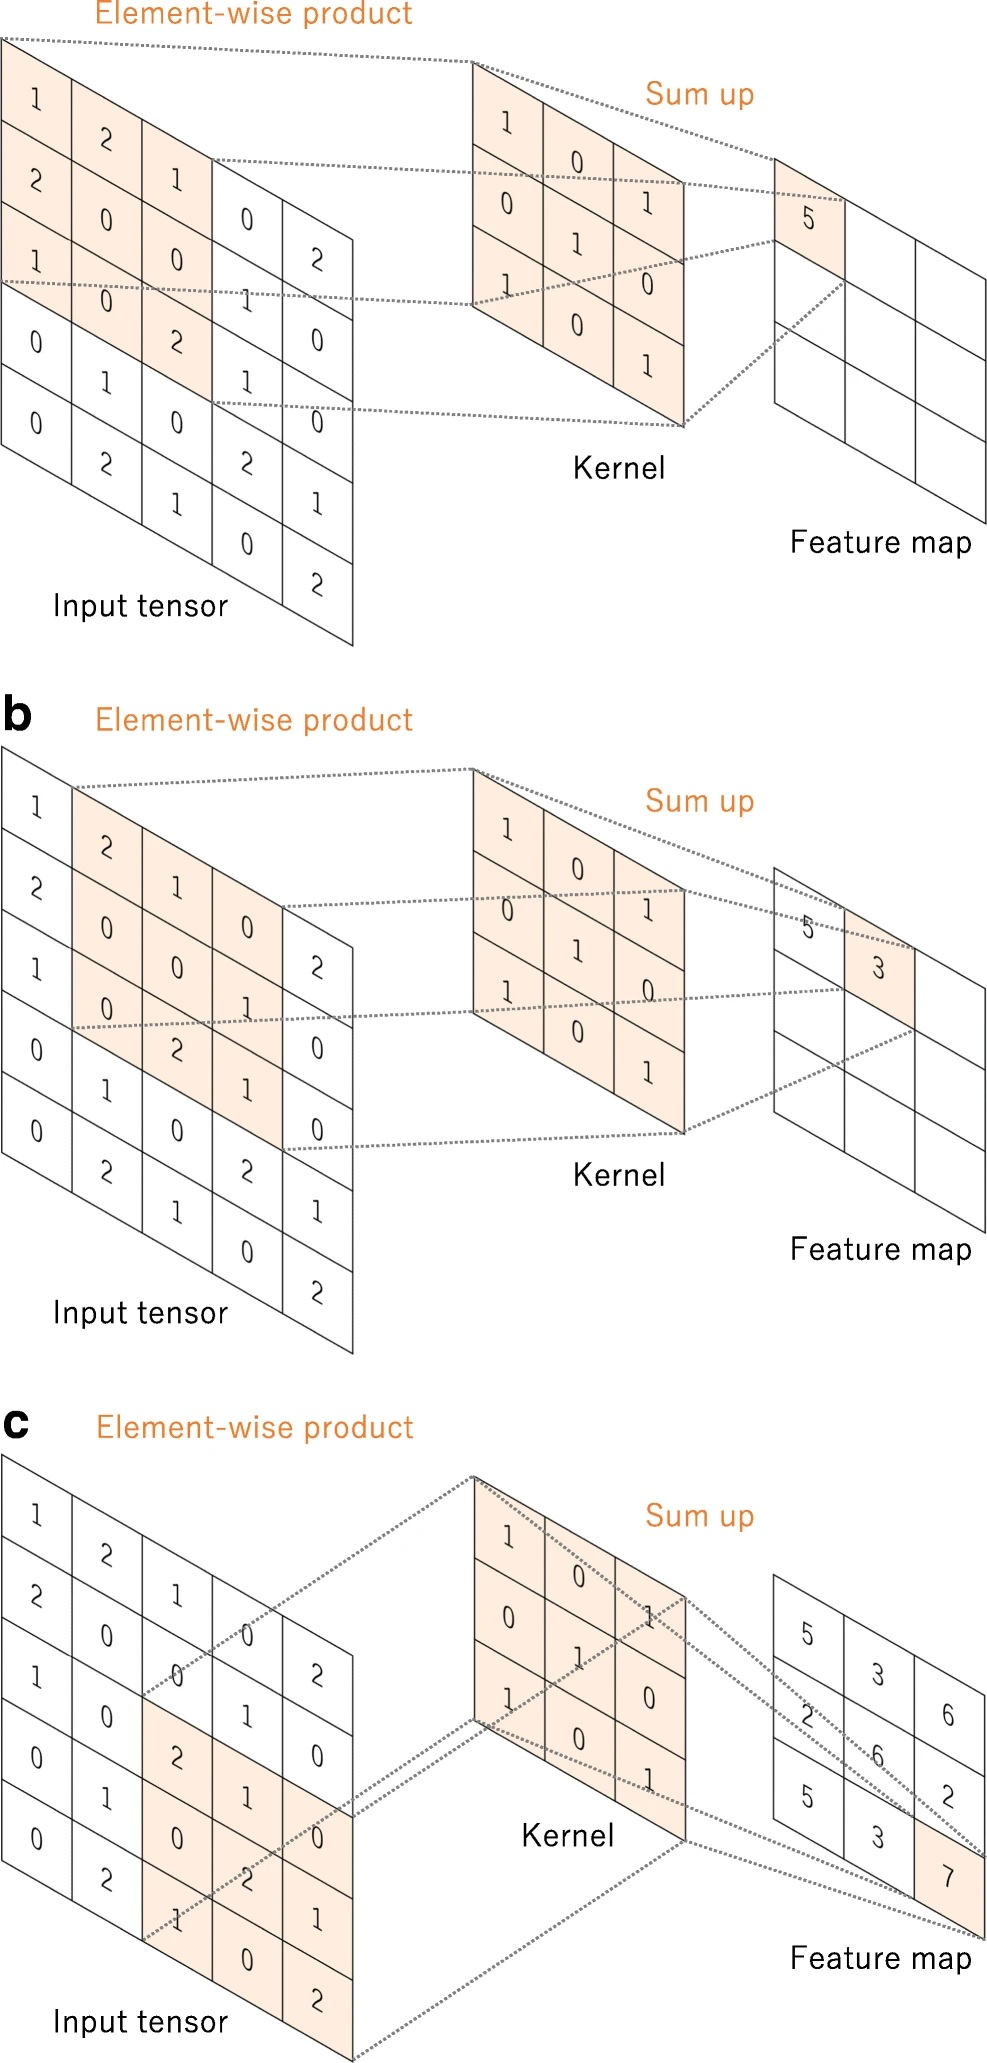
\includegraphics[scale=0.40]{images/Fundamentals/Convolution.JPG}
	    \caption[An illustration of Convolution Operation.]{\textbf{a–c} An illustration of convolution operation with no padding, kernel size $3 \times 3$ and stride $1$ \cite{articleCNNs}.}
	    
	    %A kernel is applied across the input tensor and an element-wise product between each element of the kernel and the input tensor is calculated at each location and summed to obtain the output value in the corresponding position of the output tensor, called a feature map
	    \label{fig:Convolution}
	    \end{center}
\end{figure}


\subsubsection{Activation Functions}


%The \acp{ANN} are inspired by biological neural networks present in the animal brain. Before constructing any \ac{ANN}, it is important to understand the artificial neuron model. In the figure \ref{fig:artificialNeuron} schematic diagram of an artificial neuron is illustrated. 
%A biological neuron gets excited when other neurons with different weights send electrical signals to it. The value of the electrical signal should be big enough to excite the neuron, otherwise, it will be in an inactive state. 
%The addition unit gets the linear weight sum $Z$ of the inputs and bias.
%The brain receives the stimulus from the external world. It processes the information and generates an output. A biological neuron gets excited when other neurons with different weights send electrical signals to it. The value of the electrical signal should be big enough to excite the neuron otherwise, it will be in an inactive state. It learns complex patterns by communicating with millions of neurons inside the brain. The artificial neurons work similarly to biological neurons. 

The artificial neuron is a mathematical function inspired by the neurons inside the brain and they are the basis of \acp{ANN}. The artificial neurons receive one or more weighted inputs and bias, and their sum is passed through an activation function. An artificial neuron's schematic diagram is illustrated in figure \ref{fig:artificialNeuron}, where $\{X_1, X_2, X_3, ..., X_n\}$ are the inputs to the artificial neuron, $\{W_1, W_2, W_3, ..., W_n\}$ are the weights corresponding to the inputs and $b$ is the bias. The summation symbol represents the addition unit. Inputs are fed to the neuron, they perform a linear transformation on these inputs using the weights and biases. If $X = [X_1, X_2, X_3, ..., X_n]  \in R^{n}$  and  $W = [W_1, W_2, W_3, ..., W_n] \in R^{n}$, then output $Z$ is represented as

\begin{equation}\label{linearRegression}
Z=X{W}^\intercal + b.
\end{equation}

\begin{figure}[H]
        \begin{center}
	    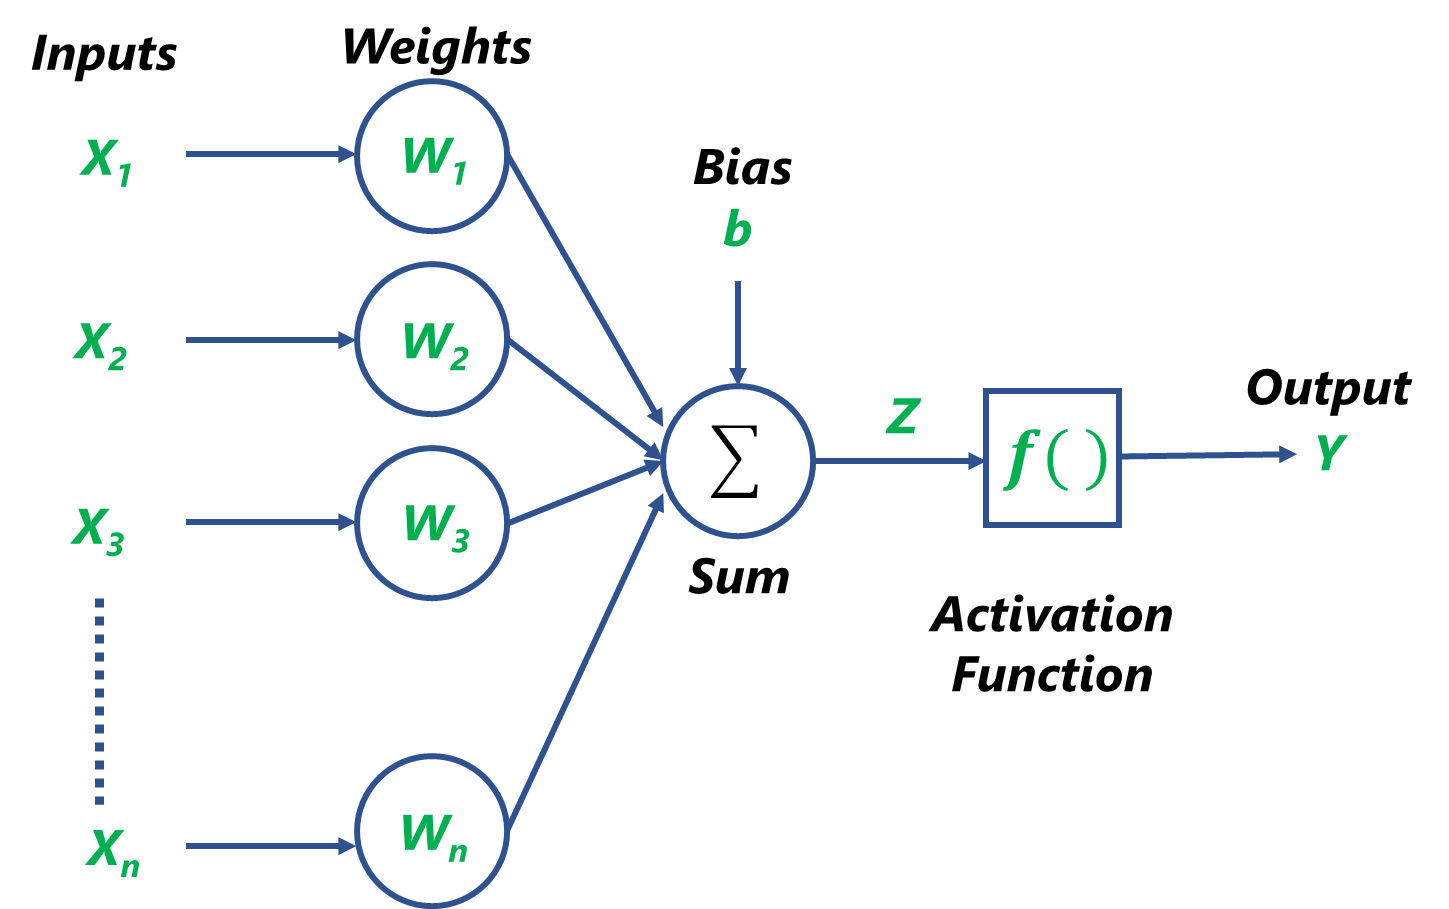
\includegraphics[scale=0.30]{images/Fundamentals/artificialNeuron.png}
	    \caption[An illustration of artificial neuron.]{An illustration of artificial neuron.}
	    \label{fig:artificialNeuron}
	    \end{center}
\end{figure}

The function $f$ is the activation function applied on $Z$.
\begin{equation}\label{artificialNeuron}
Y = f(Z).
\end{equation}

%The activation functions are important while constructing any neural network as they are mathematical functions attached to the neurons. The activation function is applied to the outputs of a linear operation like convolution. Also, they tell which of the neuron is excited or triggered in each layer of neural networks. 
%The main purpose of the activation function is to introduce non-linearity in the neural network. The equation \ref{linearRegression} performs a linear operation. This linear function gets repeated every hidden layer of the neural network. A combination of such linear functions also a linear function, equivalent to all the hidden layers collapsed into a single linear function performing linear regression. Hence, all the hidden layers become useless. Even if linear functions are easy to use, but they fail to learn complex patterns present in the data like images, speech and videos. Hence, nonlinear activation functions are used, while constructing neural networks. 

The data is fed to the input layer of the neurons in neural network, undergoes the linear operation, later, activation functions are applied in the hidden layers and output is produced. The produced output the propagated forward to next hidden layers, this is movement is called forward propagation\footnotemark. In neural networks the hidden layer lies between input layer and output layer. A simple neural network is illustrated in figure \ref{fig:ann}. The main purpose of the activation function is to introduce non-linearity in the neural network. The linear functions are easy to use, but they fail to learn complex patterns present in the data like images, speech and videos. Hence, nonlinear activation functions are used, while constructing neural networks. The nonlinear activation functions are differentiable. The neural networks learn from the errors calculated at the output layer, a differentiable nonlinear activation function is required to perform backpropagation to compute loss with respect to the weights of the neurons and optimize them using gradient descent optimization algorithm or any other optimization algorithm. 

\footnotetext{\url{https://www.analyticsvidhya.com/blog/2020/01/fundamentals-deep-learning-activation-functions-when-to-use-them/} last access: \dcdate}

\begin{figure}[H]
        \begin{center}
	    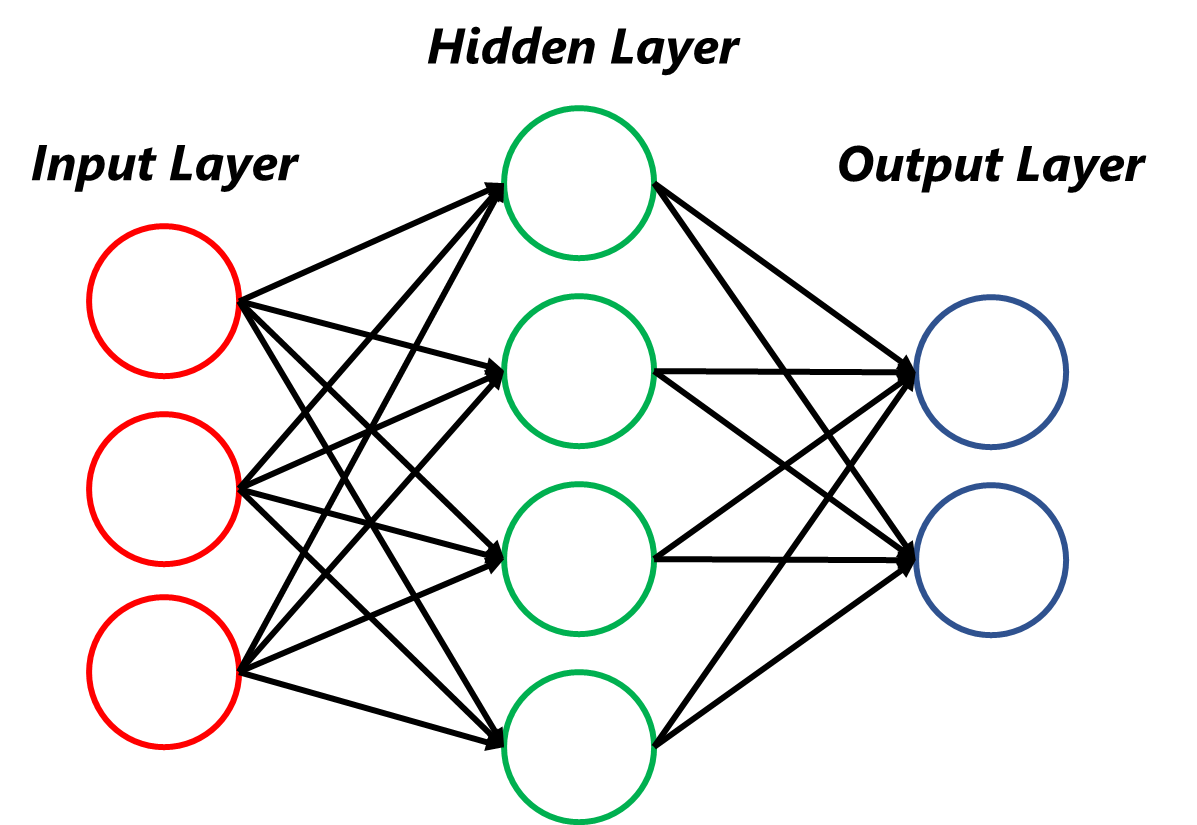
\includegraphics[scale=0.30]{images/Fundamentals/ann.png}
	    \caption[Simple neural network.]{Simple neural network}
	    \label{fig:ann}
	    \end{center}
\end{figure}

The backpropagation minimizes the error, updates the weights of neurons and enhances the accuracy and performance of the neural network. The nonlinear functions, sigmoid, hyperbolic tangent(tanh) functions ware mathematical representations of biological neuron behavior. The \ac{ReLU} is now the most commonly used nonlinear activation function, it computes the function: $f(x) = \max(0, x)$. These activation functions along with their plots are illustrated in figure \ref{fig:ActivationFunctions} \cite{LeCun.2015} \cite{NIPS2012_c399862d}.


% \cite{10.5555/3104322.3104425} \cite{ramachandran2017searching} \cite{pmlr-v15-glorot11a}.



\vspace*{0.5cm}

\begin{figure}[H]
        \begin{center}
	    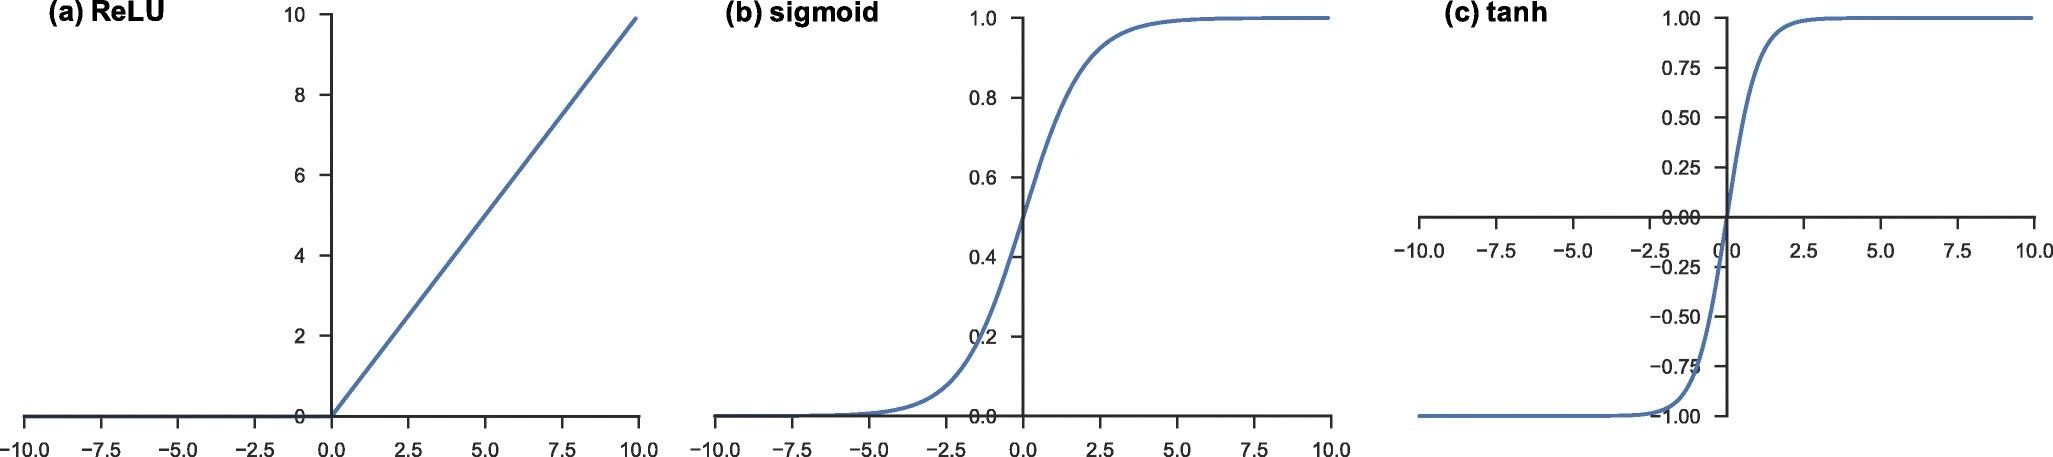
\includegraphics[scale=0.42]{images/Fundamentals/ActivationFunctions.jpg}
	    \caption[Most common nonlinear activation functions used while constructing Neural Networks.]{Most common nonlinear activation functions used while constructing neural networks: \textbf{a)} \ac{ReLU}, \textbf{b)} sigmoid and \textbf{c)} hyperbolic tangent (tanh) \cite{articleCNNs}.}
	    \label{fig:ActivationFunctions}
	    \end{center}
\end{figure}

\subsection{Pooling Layer}\label{PoolingLayer}
A pooling layer performs downsampling on feature maps to gradually reducing the spatial dimensionality, which leads to the reduction of the computational complexity and number of parameters of the neural network and controlling overfitting. Downsampling introduces translation invariance to minor shifts and distortions \cite{goodfellow2017deep}. Downsampling of feature maps can also be accomplished by using convolution layers by increasing the stride of the convolution operation across the image. But the robust and common approach of downsampling is to use a pooling layer \cite{goodfellow2017deep}. Similar to convolution operations, it uses hyperparameters like filter size, stride and padding. Also, it is common to periodically insert a pooling layer in between successive convolution layers while constructing neural networks. There two common types of pooling methods one is max pooling the other is average pooling. The max-pooling considers the most activated (maximum) value in each input patch of the feature map. The average pooling averages values in each input patch of the feature map \cite{10.1007/978-3-642-15825-4_10}.

\subsubsection{Max Pooling}
Max pooling is the most common and popular type of pooling operation. The max-pooling operation is independently operated at every depth slice of the input and resized spatially. Commonly, max-pooling filters are of size $2 \times 2$ and applied with a stride of 2. The max-pooling operation extracts small patches of given filter size from the input feature maps and outputs the maximum value in every patch discarding others (figure \ref{fig:PoolingLayer}) \cite{goodfellow2017deep}. The spatial dimension of feature maps is reduced by a factor of two by discarding 75\% of its activations \cite{kumar2018ordinal}. The height and width dimension of the features maps is reduced but the depth dimension remains unchanged. Pooling operations with larger filter sizes are too destructive and it's worth noting that max-pooling layers do not have learnable parameters \cite{articleCNNs}.


\begin{figure}[H]
        \begin{center}
	    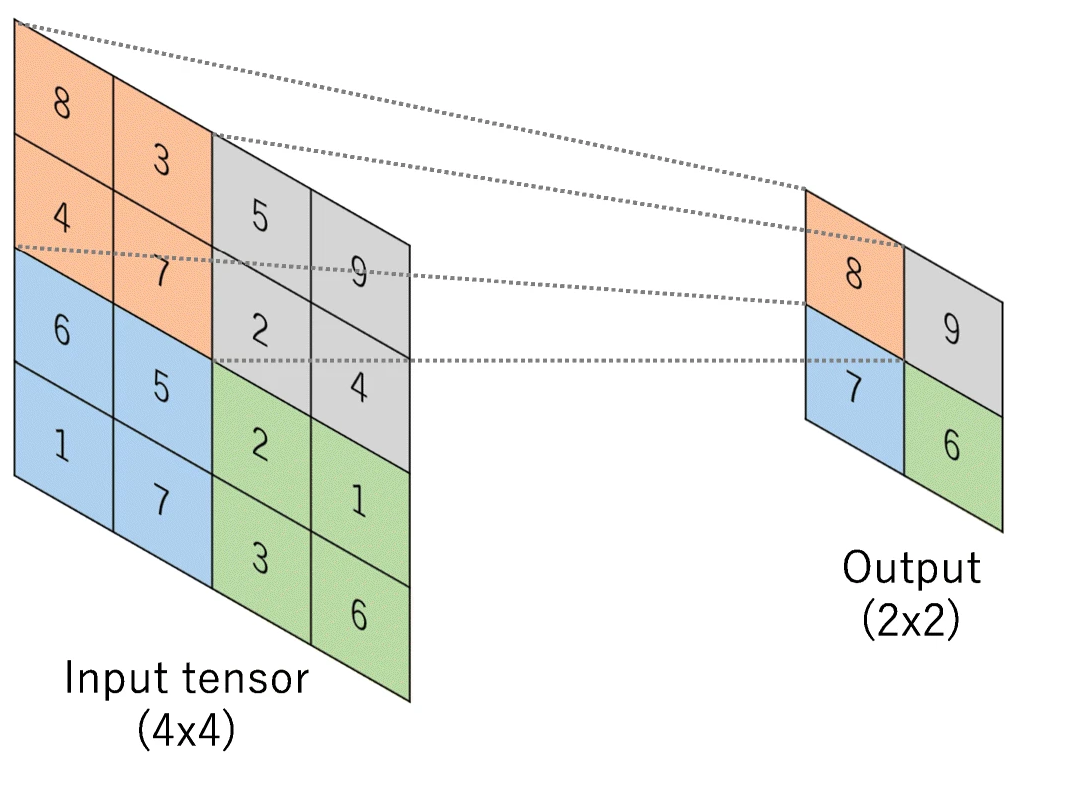
\includegraphics[scale=0.50]{images/Fundamentals/PoolingLayer.png}
	    \caption[An illustration of Max Pooling Operation.]{An illustration of max pooling operation with a filter size of $2 \times 2$, no padding and stride 2. Max pooling operation extracts $2 \times 2$ patches from the input tensors and outputs the maximum value in each patch by ignoring the remaining values. The spatial dimension of an input tensor is downsampled by a factor of 2 \cite{articleCNNs}.}
	    \label{fig:PoolingLayer}
	    \end{center}
\end{figure}


\subsubsection{Global Average Pooling}
There is another type of pooling operation called global average pooling. It performs an extreme type of downsampling. It downsamples a feature map of size $height\ \times width\ \times\ depth$ into a $1\ \times 1\ \times\ depth$ array by averaging all the elements present in the feature map by keeping depth dimension unchanged. This operation is applied only once before fully connected layers. There are some benefits of using global average pooling: a)  It reduces the number of learnable parameters. b) allows the \ac{CNN} to consider inputs of variable size \cite{articleCNNs} \cite{lin2014network}. c) It is intended to replace fully connected layers, the idea is to generate one feature map for each class, in the classification task, as they provide robust spatial information and the resulting vector can easily be fed to the softmax layer\footnotemark.

\footnotetext{\url{https://paperswithcode.com/method/global-average-pooling/} last access: \dcdate}





\subsection{Fully Connected Layer}

%In neural networks, ``fully connected layers are those layers where all the inputs from one layer are connected to every neuron of the next layer'' \cite{articleCNNs}. 

The final output feature map of convolution layers or pooling layers is flattened and the output is transformed into a \ac{1D} vector. The flattened output is connected to one or more fully connected layers. The fully connected layers are also called dense layers, where every input is connected to every output by a learnable weight \cite{articleCNNs}. A fully connected layer performs multiplication between the input and weight matrix then adds a bias vector \cite{articleCNNs}. Equation \ref{artificialNeuron} represents the task of each neuron in a fully connected layer. Each fully connected layer is followed by a nonlinear activation function, for example, \ac{ReLU}. As already described, the nonlinear activation function helps neurons learn complex patterns. The features present in an image are extracted using convolution layers and downsampled by pooling layers. Next, extracted features are mapped through fully connected layers to the final output of the neural network, determining the probability for each class in classification tasks. Usually, the number of output nodes in the fully connected layer is equal to the number of classes \cite{articleCNNs}. The last fully connected layer's activation function is usually different than others. Each task chooses a suitable activation function. Often, in binary classification tasks sigmoid activation function is used. For example, logistic regression, models the probabilities for binary classification tasks using the sigmoid activation function\footnotemark. The softmax activation function is widely used in multiclass classification tasks. The output of the last fully connected layers are normalized into target class probabilities by the softmax activation function, in the classification tasks. The probability of each class ranges between 0 and 1 and the sum of all target class probabilities is 1 \cite{articleCNNs}.


\footnotetext{\url{https://machinelearningmastery.com/choose-an-activation-function-for-deep-learning/} last access: \dcdate}






























%%%%%%%%%%%%%%%%%%%%%%%%%%%%%%%%%%%%%%%%%%%%%%%%%%%%%%%%%%%%%%%%%%%%%%%%%%%%%%%%%%%%%%%%%%%%%%%%%%%%%%%%%%%%%%%%%%%%%%%%%%%%%%%%%%%%%%%%%


\begin{comment}
\begin{center}
\begin{table}[H]
    \begin{center}
    \begin{tabular}{p{0.40\linewidth} p{0.40\linewidth}} 
        \toprule
        Task & Last layer activation function \\ %[1.0ex] 
        \midrule
        Binary classification & Sigmoid\\ %[1.0ex] 
        \midrule
        Multiclass single-class classification & Softmax \\ %[1.0ex]
        \midrule
        Multiclass multiclass classification & Sigmoid \\ %[1.0ex]
        \midrule
        Regression to continuous values & Identity \\ %[1.0ex]
        \bottomrule
    \end{tabular}
    \caption{A list of commonly applied last layer activation functions for various tasks.}
    \label{table:activationfunction}
    \end{center}
\end{table}
\end{center}
\end{comment}


%Another pooling operation worth noting is a global average pooling \cite{lin2014network}. An extreme type of downsampling is performed by global average pooling. Eventually, global average pooling downsamples a feature map with a size of height $\times$ width into a $1 \times 1$ array by simply taking the average of all the elements in each feature map while maintaining the depth of feature maps. Before the fully connected layers, this operation is usually applied only once \cite{articleCNNs}. The following are the benefits of using global average pooling: (1) it reduces the number of learnable parameters and (2) it allows the \ac{CNN} to accept inputs of variable size. Before the fully connected layers, this operation is usually performed only once. The following are some of the benefits of using global average pooling: (1) the number of learnable parameters is decreased and (2) allows the CNN to consider inputs of variable size

%In recent years tremendous interest in deep learning has developed. The most successful algorithm among numerous deep learning models is \acp{CNN}. It is a class of artificial neural networks. It has been a prevailing method in solving computer vision tasks since the extraordinary results were shared on the object recognition competition known as the \ac{ILSVRC} in 2012 [ \cite{russakovsky2015imagenet}, \cite{NIPS2012_4824}]. It has been a popular method in solving computer vision tasks since the remarkable performance at the object recognition competition known as the \ac{ILSVRC} in 2012 [ \cite{russakovsky2015imagenet}, \cite{NIPS2012_4824}]. 
%\footnote{A convolution is a mathematical operation that slides one function over another and measures the integral of their pointwise multiplication. It has deep connections with the Fourier transform and the Laplace transform and is heavily used in signal processing. Convolutional layers actually use cross-correlations, which are very similar to convolutions (see \url{https://homl.info/76} for more details) \cite{10.5555/3153997}last access: 08.05.2021.}


%\acp{CNN} combinations of several building blocks like convolution layers, pooling layers (e.g., max pooling, global average pooling) and fully connected layers. These building blocks are stacked on each other. With a loss function through forward propagation on a training dataset, a model’s performance under particular kernels and weights is calculated. The learnable parameters, like kernels and weights, are updated as per the loss value through backpropagation using a gradient descent optimization algorithm \cite{ruder2017overview}. The ReLU notation stands for the rectified linear unit. It is an activation function \ref{fig:ActivationFunctions} \cite{articleCNNs}.

\begin{comment}
\begin{center}
\begin{table}
    \begin{tabular}{p{0.25\linewidth} p{0.15\linewidth} p{0.50\linewidth}} 
        \toprule
        & Parameters & Hyperparameters\\ %[1.0ex] 
        \midrule
        Convolution layer & Kernels & Kernel size, number of kernels, stride, padding, activation function \\ %[1.0ex]
        \midrule
        Pooling layer & None & Pooling method, filter size, stride, padding \\ %[1.0ex]
        \midrule
        Fully connected layer & Weights & Number of weights, activation function \\ %[1.0ex]
        \midrule
        Others & & Model architecture, optimizer, learning rate, loss function, mini-batch size, epochs, regularization, weight initialization, dataset splitting\\% [1.0ex]
        \bottomrule
    \end{tabular}
    \caption{A list of parameters and hyperparameters in a convolutional neural network (\ac{CNN}).}
    \label{table:hyperparametersCNN}
\end{table}
\end{center}
\end{comment}

%Max pooling is the most common form of pooling operation, which extracts patches from the input feature maps, outputs the maximum value in each patch and discards the rest (figure \ref{fig:PoolingLayer}). In practice, a max pooling with a size $2 \times 2$ filter and a stride of 2 is widely used. The spatial dimension of feature maps is reduced by a factor of two. The depth dimension of feature maps, unlike the height and width dimensions, does not change.

\begin{comment}
The discriminator in a \ac{GAN} is a binary classifier. It tries to classify between real data and the data generated by the generator. The discriminator can use any network architecture which is suitable to the kind of data it's classifying. The  training data of the discriminator comes from two sources: a) Real Data Samples. During training, the discriminator uses these samples as positive instances. b) Fake Data Samples generated by the generator. The discriminator uses these samples as negative instances during training. In figure \ref{fig:discriminatorTraining}, the two ``Sample" boxes represent these two data sources feeding into the discriminator.


The generator does not train when the discriminator is training. The generator's weights remain unchanged while it generates samples to train the discriminator. The discriminator is connected to two loss functions. The discriminator completely ignores the generator loss and just uses the discriminator loss during its training. The generator loss is used during generator training to update its weights. The coming section \ref{TheGeneratorSubSection} describes why the generator loss connects to the discriminator. During the discriminator training process: a) Discriminator classifies both real data and fake data generated from the generator. b) The discriminator loss penalizes the discriminator for wrongly classifying a real instance as fake or a fake instance as real. c) Through backpropagation, the discriminator updates its weights using the discriminator loss through the discriminator network.
\end{comment}

\begin{comment}
The generator part of a \ac{GAN} learns to create fake data by receiving backpropagation loss from the discriminator. Slowly it learns and trains to make the discriminator classify its fake output as real. Generator training requires a closer alliance between the generator and the discriminator as compared to the discriminator training requires. The part of the \ac{GAN} that trains the generator includes: a) Random input data. b) Generator network, which transforms the random input data into plausible data. c) Discriminator network, which classifies the generated data. d) Discriminator output. e) Generator loss, which penalizes the generator for failing to fool the discriminator. Neural networks need some form of input data, like an example for classification or to predict about. But what to consider as an input for a neural network that outputs entirely new data instances? In its most fundamental form, a \ac{GAN} takes random noise as its input. The generator then transforms this random noise into a plausible output. By introducing random noise, \ac{GAN} can generate a wide variety of data, sampling from different places in the target distribution. Investigations suggest that the distribution of the noise doesn’t matter much, therefore it is possible to choose something easy to sample from, as a uniform distribution. For simplicity, the distribution from which the noise is sampled is usually of a smaller dimension than the dimensionality of the output distribution. To train a neural network, its weights are updated to reduce the error or loss of its output.  In \ac{GAN}, however, the generator is not directly connected to the loss that is required to update its weights. The discriminator produces the generator loss as the generator feeds into the discriminator network. The generator loss penalizes the generator for generating a sample that the discriminator network classifies as fake. This extra piece of the implementation must be included in backpropagation. The backpropagation adjusts the weights in the appropriate direction by calculating the weight’s impact on the output — how the output would change if you updated the weights. But the impact of a generator weight depends on the discriminator weights it feeds into. So generator loss is backpropagated from the output of the discriminator to the generator. Means gradients flow back through the discriminator into the generator. 


At the same time, the discriminator will not change during generator training. Attempting to hit a moving target would make a complicated problem even difficult for the generator. The generator is trained with the following procedure: 1) Random noise input to the generator. 2) Generator produces output from sampled random noise. 3) The discriminator determines whether the generator output is “Real” or “Fake”. 4) Calculate loss from discriminator classification. 5) Backpropagate the generator loss through both the discriminator and generator to obtain gradients. 6) Use the gradients to update only the generator's weights.
\end{comment}

\begin{comment}
The \ac{GAN} has two training models one is a generator and another is a discriminator. The generator learns to generate plausible data. The discriminator always aims to reject samples produced by the generator as the generated samples are negative training samples for the discriminator. Throughout the training, the discriminator learns to distinguish the generator's fake data from real data. When the generator produces implausible results the discriminator penalizes it. Once the training starts, the generator generates fake data and the discriminator learns to rejects the data by saying the generator that it's fake data. As training progresses, the generator learns to produce the output that can fool the discriminator. Lastly, if generator training is successful, the discriminator gets bad at telling the difference between real data and fake data generated by the generator. The discriminator starts to classify fake data as real and its accuracy decreases. Ultimately, the generator will start producing plausible data. Both the generator and the discriminator are neural networks. The generator's output is connected directly to the discriminator's input. The discriminator's classification provides the loss that the generator uses to update its weights using backpropagation.

\subsection{The Discriminator}\label{TheDiscriminatorSubSection}

\vspace*{-0.7cm}
\begin{figure}[H]
        \begin{center}
	    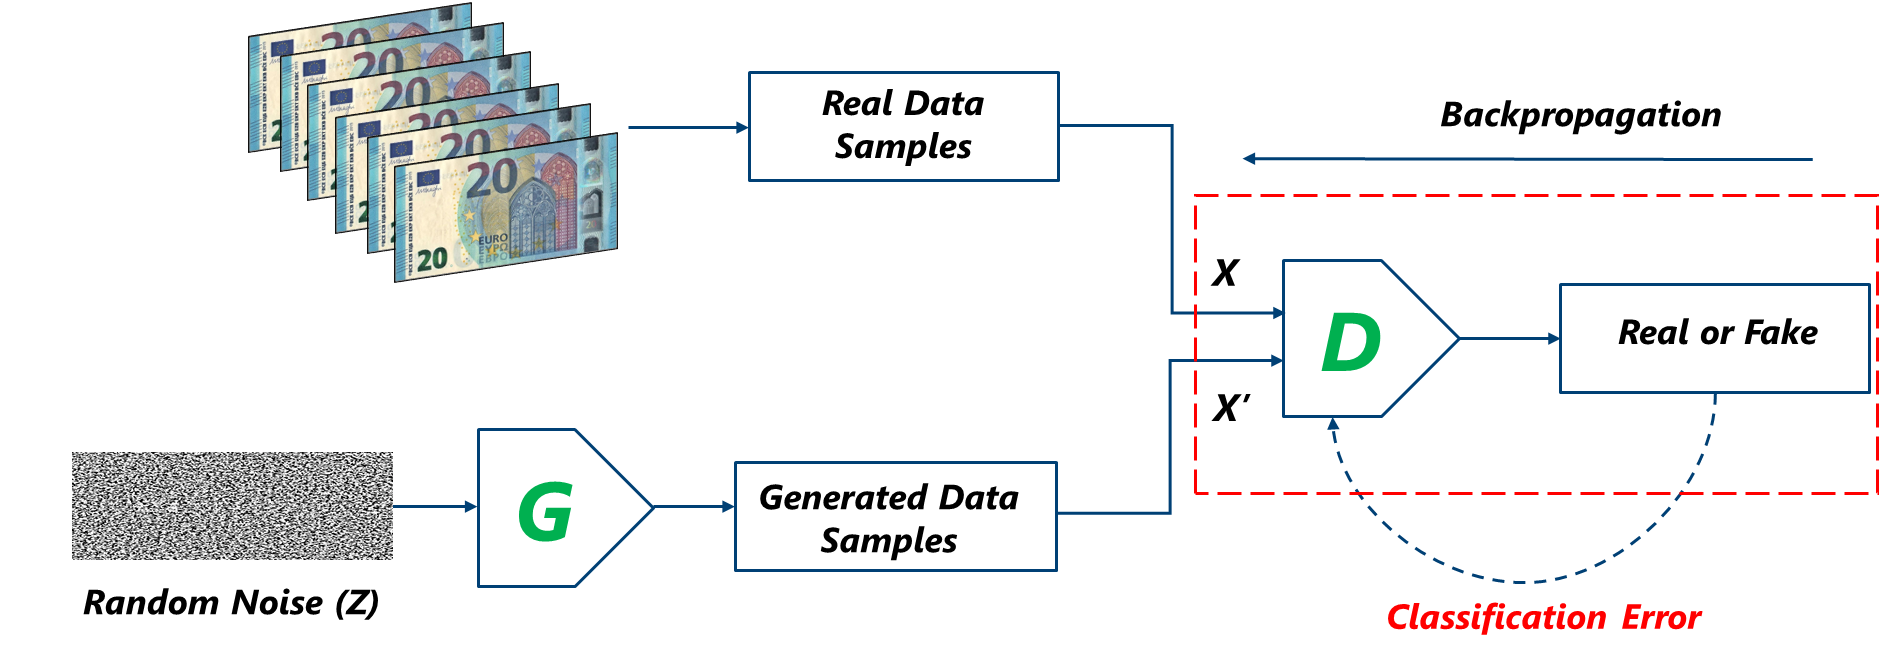
\includegraphics[scale=0.45]{images/discriminatorTraining.png}
	    \caption[Illustartion of the training of the discriminator $D$ using backpropagation.]{Training of the discriminator $D$ using backpropagation.}
	    \label{fig:discriminatorTraining}
	    \end{center}
\end{figure}

The discriminator in a \ac{GAN} is a binary classifier. It tries to classify between real data and the data generated by the generator. The discriminator can use any network architecture which is suitable to the kind of data it's classifying. The  training data of the discriminator comes from two sources: a) Real Data Samples. During training, the discriminator uses these samples as positive instances. b) Fake Data Samples generated by the generator. The discriminator uses these samples as negative instances during training. In figure \ref{fig:discriminatorTraining}, the two ``Sample" boxes represent these two data sources feeding into the discriminator. The generator does not train when the discriminator is training. The generator's weights remain unchanged while it generates samples to train the discriminator. The discriminator is connected to two loss functions. The discriminator completely ignores the generator loss and just uses the discriminator loss during its training. The generator loss is used during generator training to update its weights. The coming section \ref{TheGeneratorSubSection} describes why the generator loss connects to the discriminator. During the discriminator training process: a) Discriminator classifies both real data and fake data generated from the generator. b) The discriminator loss penalizes the discriminator for wrongly classifying a real instance as fake or a fake instance as real. c) Through backpropagation, the discriminator updates its weights using the discriminator loss through the discriminator network.





\subsection{The Generator}\label{TheGeneratorSubSection}

%\vspace*{1.5cm}
\begin{figure}[H]
    \begin{center}
	\includegraphics[scale=0.30]{images/generatorTraining.png}
	\caption[Training Generator $G$ using backpropagation]{Training Generator $G$ using backpropagation.}
	\label{fig:generatorTraining}
	\end{center}
\end{figure}

The generator part of a \ac{GAN} learns to create fake data by receiving backpropagation loss from the discriminator. Slowly it learns and trains to make the discriminator classify its fake output as real. Generator training requires a closer alliance between the generator and the discriminator as compared to the discriminator training requires. The part of the \ac{GAN} that trains the generator includes: a) Random input data. b) Generator network, which transforms the random input data into plausible data. c) Discriminator network, which classifies the generated data. d) Discriminator output. e) Generator loss, which penalizes the generator for failing to fool the discriminator. Neural networks need some form of input data, like an example for classification or to predict about. But what to consider as an input for a neural network that outputs entirely new data instances? In its most fundamental form, a \ac{GAN} takes random noise as its input. The generator then transforms this random noise into a plausible output. By introducing random noise, \ac{GAN} can generate a wide variety of data, sampling from different places in the target distribution. Investigations suggest that the distribution of the noise doesn’t matter much, therefore it is possible to choose something easy to sample from, as a uniform distribution. For simplicity, the distribution from which the noise is sampled is usually of a smaller dimension than the dimensionality of the output distribution. To train a neural network, its weights are updated to reduce the error or loss of its output.  In \ac{GAN}, however, the generator is not directly connected to the loss that is required to update its weights. The discriminator produces the generator loss as the generator feeds into the discriminator network. The generator loss penalizes the generator for generating a sample that the discriminator network classifies as fake. This extra piece of the implementation must be included in backpropagation. The backpropagation adjusts the weights in the appropriate direction by calculating the weight’s impact on the output — how the output would change if you updated the weights. But the impact of a generator weight depends on the discriminator weights it feeds into. So generator loss is backpropagated from the output of the discriminator to the generator. Means gradients flow back through the discriminator into the generator. At the same time, the discriminator will not change during generator training. Attempting to hit a moving target would make a complicated problem even difficult for the generator. The generator is trained with the following procedure: 1) Random noise input to the generator. 2) Generator produces output from sampled random noise. 3) The discriminator determines whether the generator output is “Real” or “Fake”. 4) Calculate loss from discriminator classification. 5) Backpropagate the generator loss through both the discriminator and generator to obtain gradients. 6) Use the gradients to update only the generator's weights.

\end{comment}


\newpage

\chapter{Methodology}
    \label{methodology}
    %\noindent
\justifying
\setlength{\parskip}{1em}

%This chapter describes the methodology of the proposed image-to-image translation application, \ac{CycleGAN}(Cycle-Consistent Adversarial Network). In acp\{CycleGAN}, also, it describes the algorithm of the \ac{CycleGAN}. It explains the loss functions used to optimize the model, along with the final objective function.
%In this chapter, the methodology of the proposed image-to-image translation application. In section \ref{ProposedApproach}, the proposed approach is pictorially described and theoretically explained. In section \ref{CycleConsistentAdversarialNetworks}, the mathematics behind \ac{CycleGAN} is discussed thoroughly along with loss functions and objective functions. Also, the algorithm of the \ac{CycleGAN} described in section \ref{CycleGANAlgorithm}.

%This chapter describes the unpaired image-to-image translation method \ac{CycleGAN}. In this thesis \{CycleGAN} is used to implement image-to-image translation application.
 %and the loss functions used to optimize the model, including the final objective function. In \ac{CycleGAN}, the cycle-consistency loss function is used to unpaired image-to-image translation. The least-square loss is effective for stable learning and avoiding mode collapse and the identity mapping loss is beneficial for preserving the color of the images after transformation. The section \ref{CycleGANAlgorithm} presents the algorithm of \ac{CycleGAN}.

%$X$ is the source domain and $Y$ is the target domain. The domain $X$ represents synthetic data distribution and domain $Y$ represents real data distribution. The synthetic data distribution consists of synthetic document images created using empty form templates and handwritten crops. The real data distribution consists of the real document images. 

%\section{Proposed Approach}\label{ProposedApproach}

%The proposed method for unpaired image-to-image translation is implemented using \ac{CycleGAN}.

%The final objective is achieved using three loss functions. The cycle-consistency loss to prevent the learned mappings functions $G$ and $F$ from contradicting each other. It enables \ac{CycleGAN} to learn transform images within the context \cite{zhu2020unpaired}. The least-square loss optimizes generators and discriminators \cite{mao2017squares}. The identity mapping loss to preserve the color of the input images \cite{zhu2020unpaired}.



This chapter describes the unpaired image-to-image translation method \ac{CycleGAN}. In this thesis, \ac{CycleGAN} is used to implement an image-to-image translation application. This application transforms synthetic document images into realistic document images. The application model is optimized using cycle-consistency loss, least-square loss and identity mapping loss. These loss functions are briefly described in this chapter and section \ref{CycleGANAlgorithm} presents the algorithm of \ac{CycleGAN}.


\begin{comment}
\begin{figure}[H]
  \centering
  \begin{minipage}[b]{1.0\textwidth}
    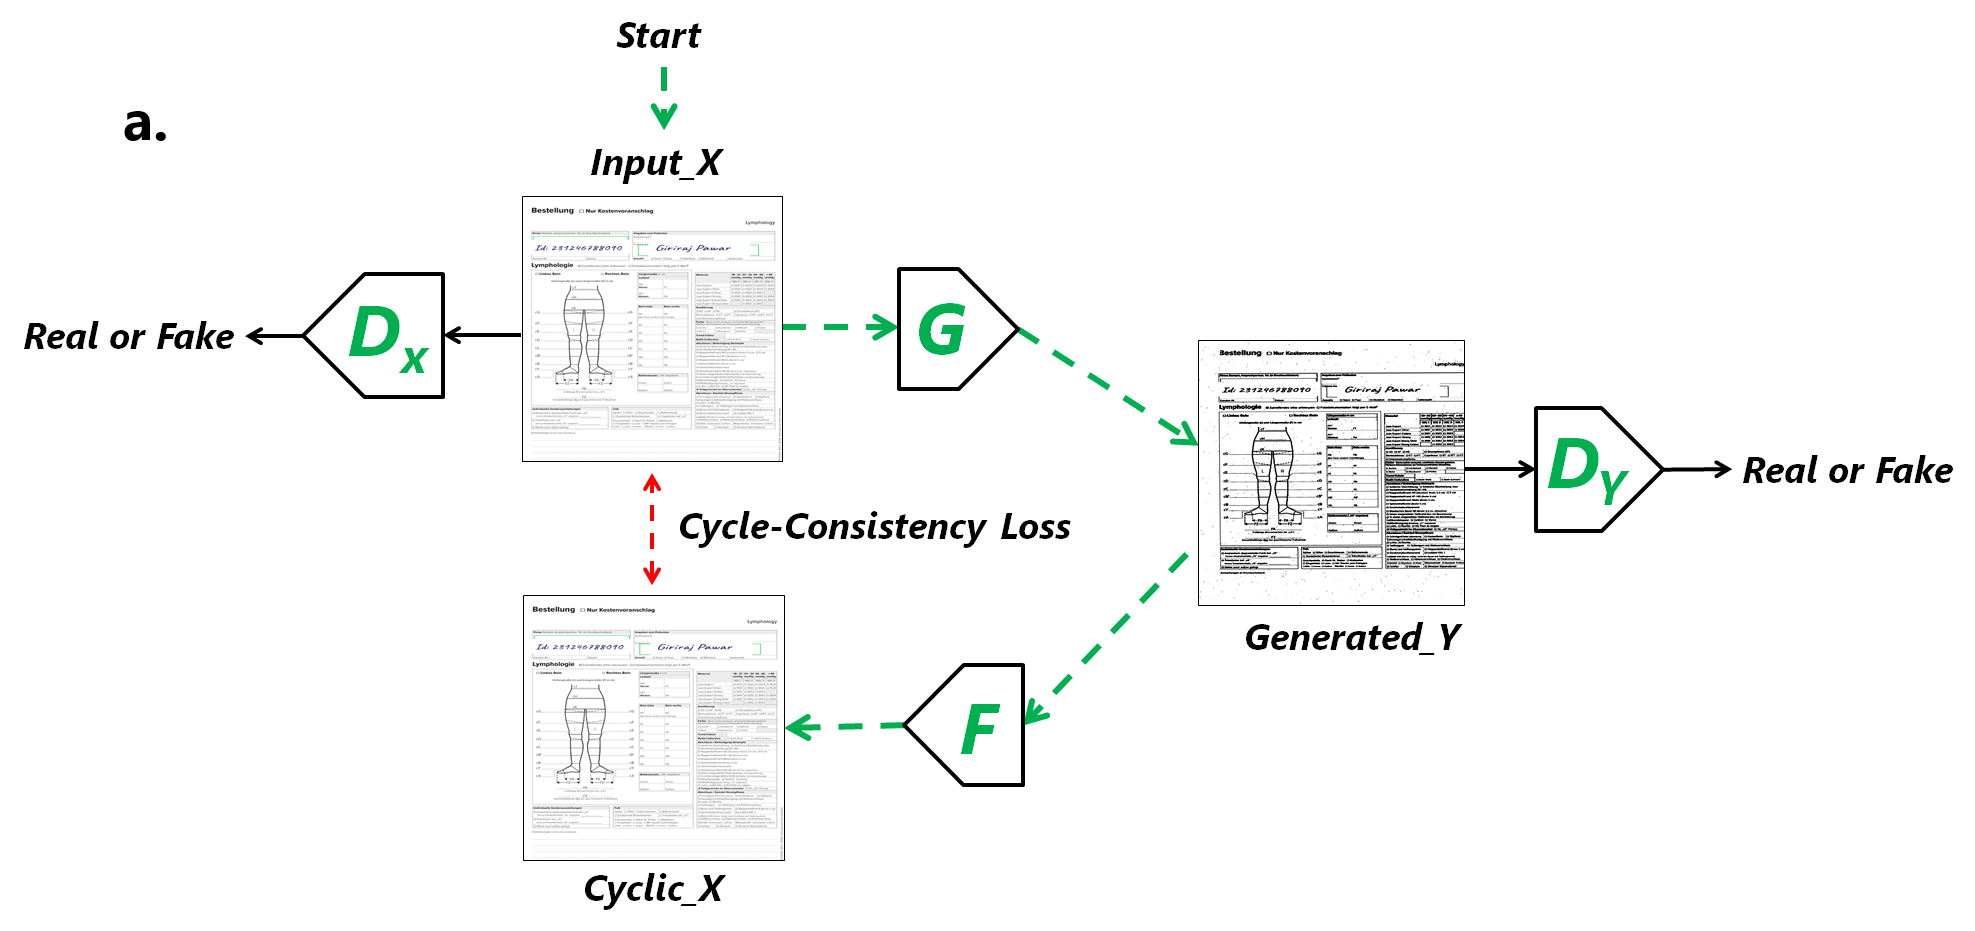
\includegraphics[width=\textwidth]{images/Methodology/Gxy.png}
  \end{minipage}
  \vfill
  \begin{minipage}[b]{1.0\textwidth}
    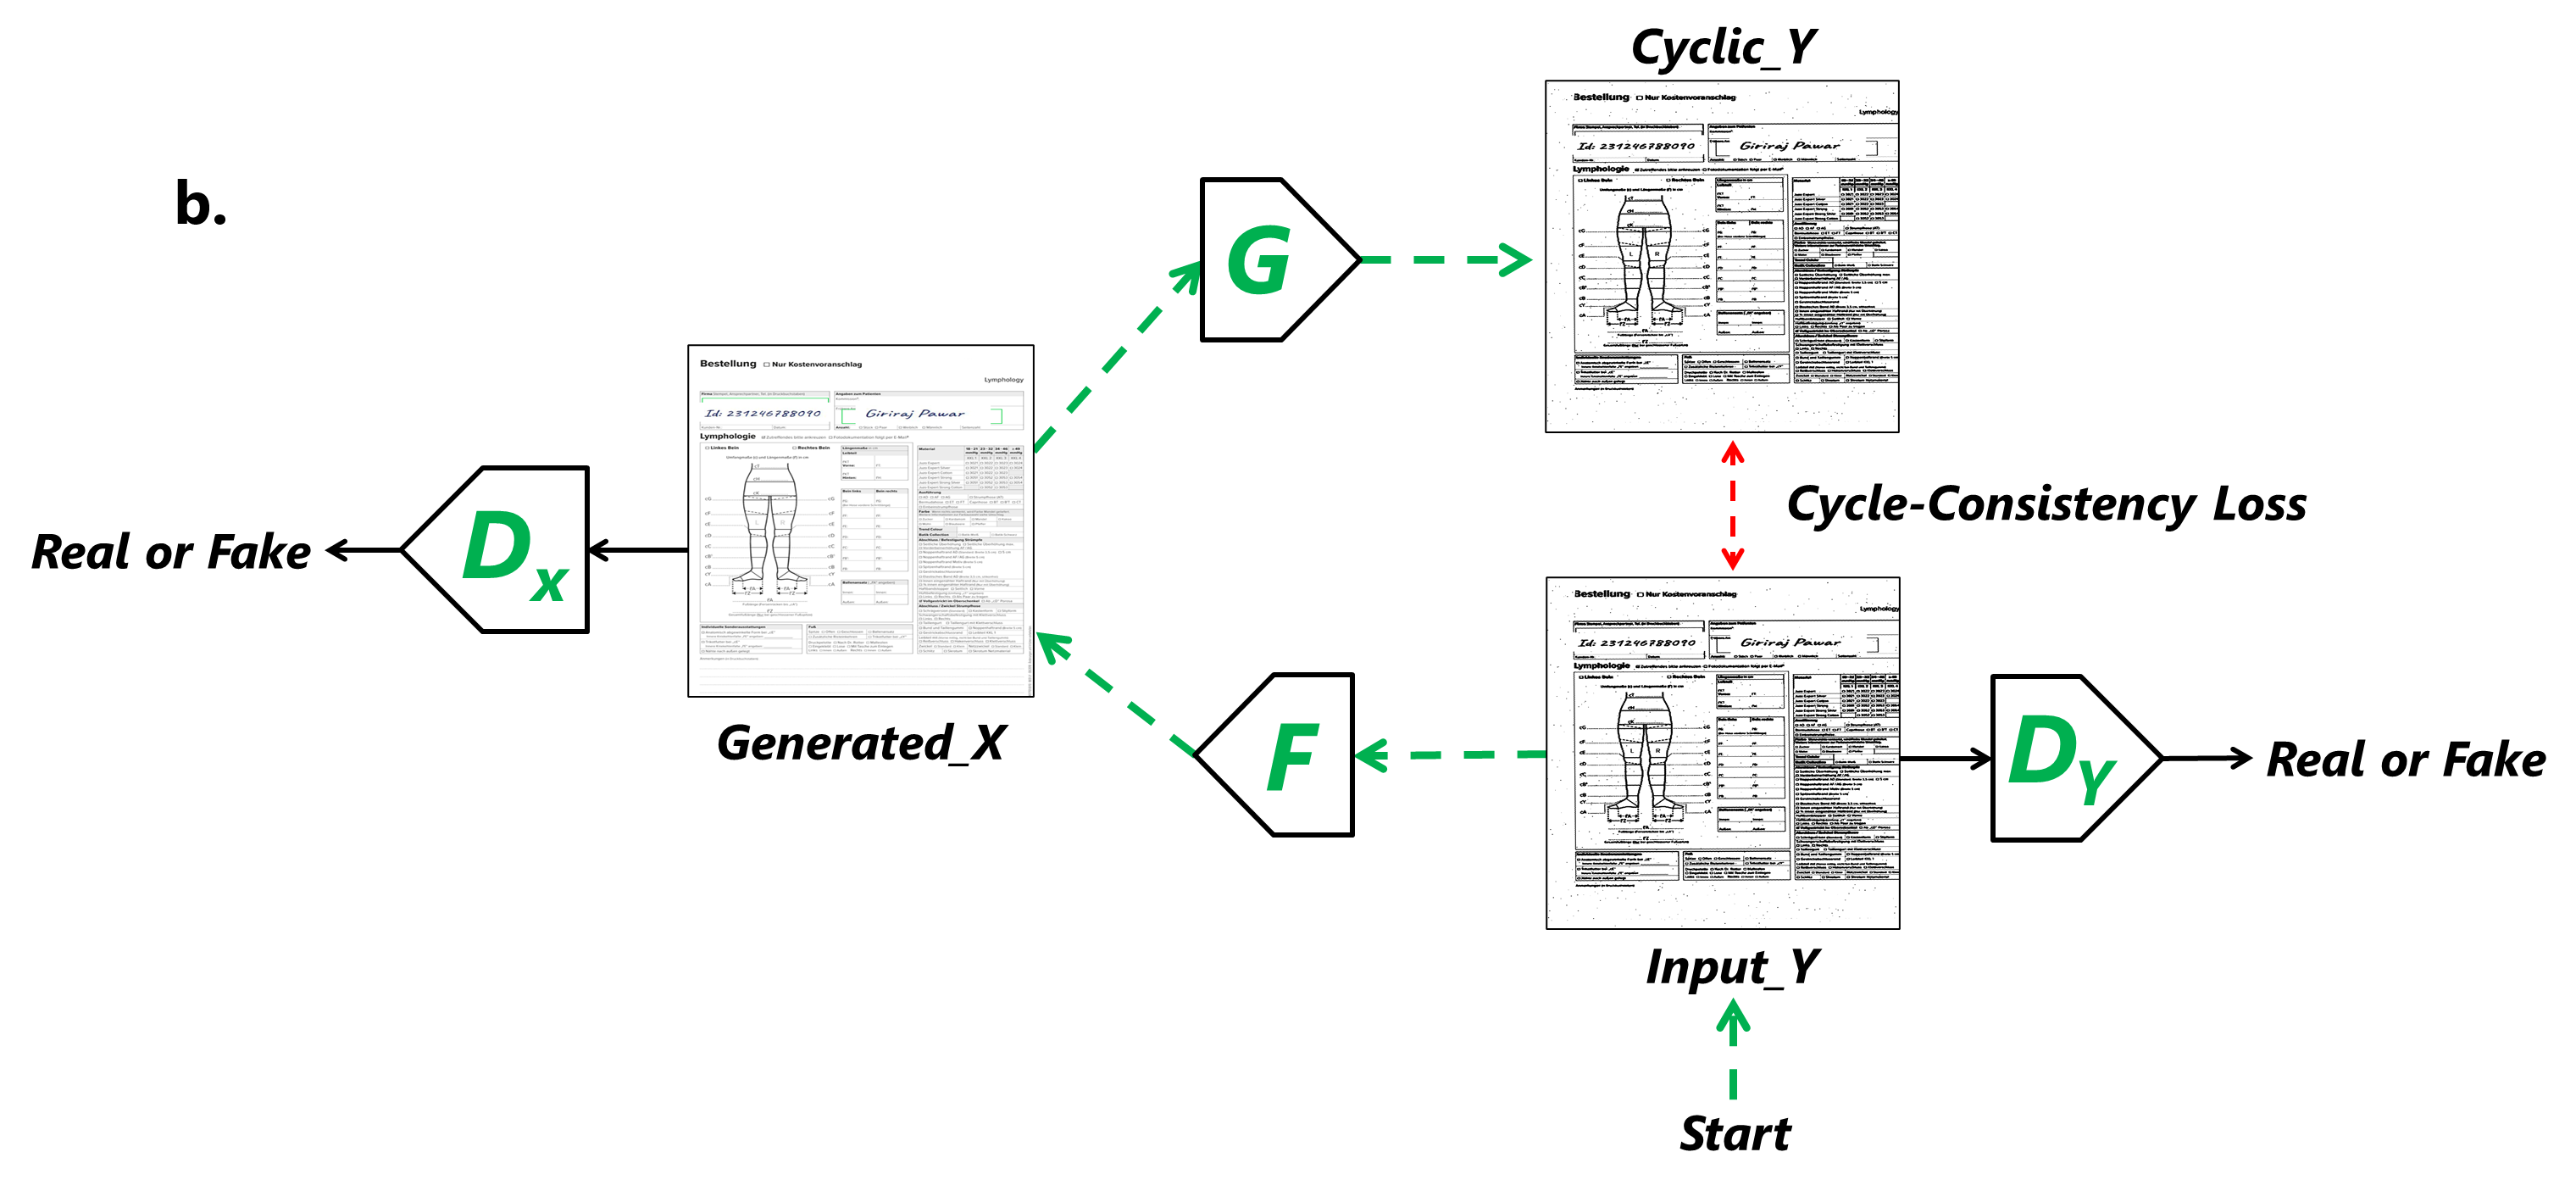
\includegraphics[width=\textwidth]{images/Methodology/Fyx.png}
  \end{minipage}
  \caption[An illustration of the proposed image-to-image translation application using \ac{CycleGAN}, for transforming synthetic document images into real document images and vice versa.]{An illustration of the proposed image-to-image translation application using \ac{CycleGAN}, for transforming synthetic document images into real document images and vice versa. It consists of two generators, $G$ and $F$ which map synthetic document images to real document images and real document images to synthetic document images, respectively, minimizing cycle-consistency loss \cite{zhu2020unpaired}. It also contains two discriminators $D_X$ and $D_Y$ which acts as the adversary and reject images generated by respective generators \cite{zhu2020unpaired}.}
  \label{fig:GxyFyx}
\end{figure}
\end{comment}

\begin{figure}[H]
  \centering
  \begin{minipage}[b]{0.98\textwidth}
    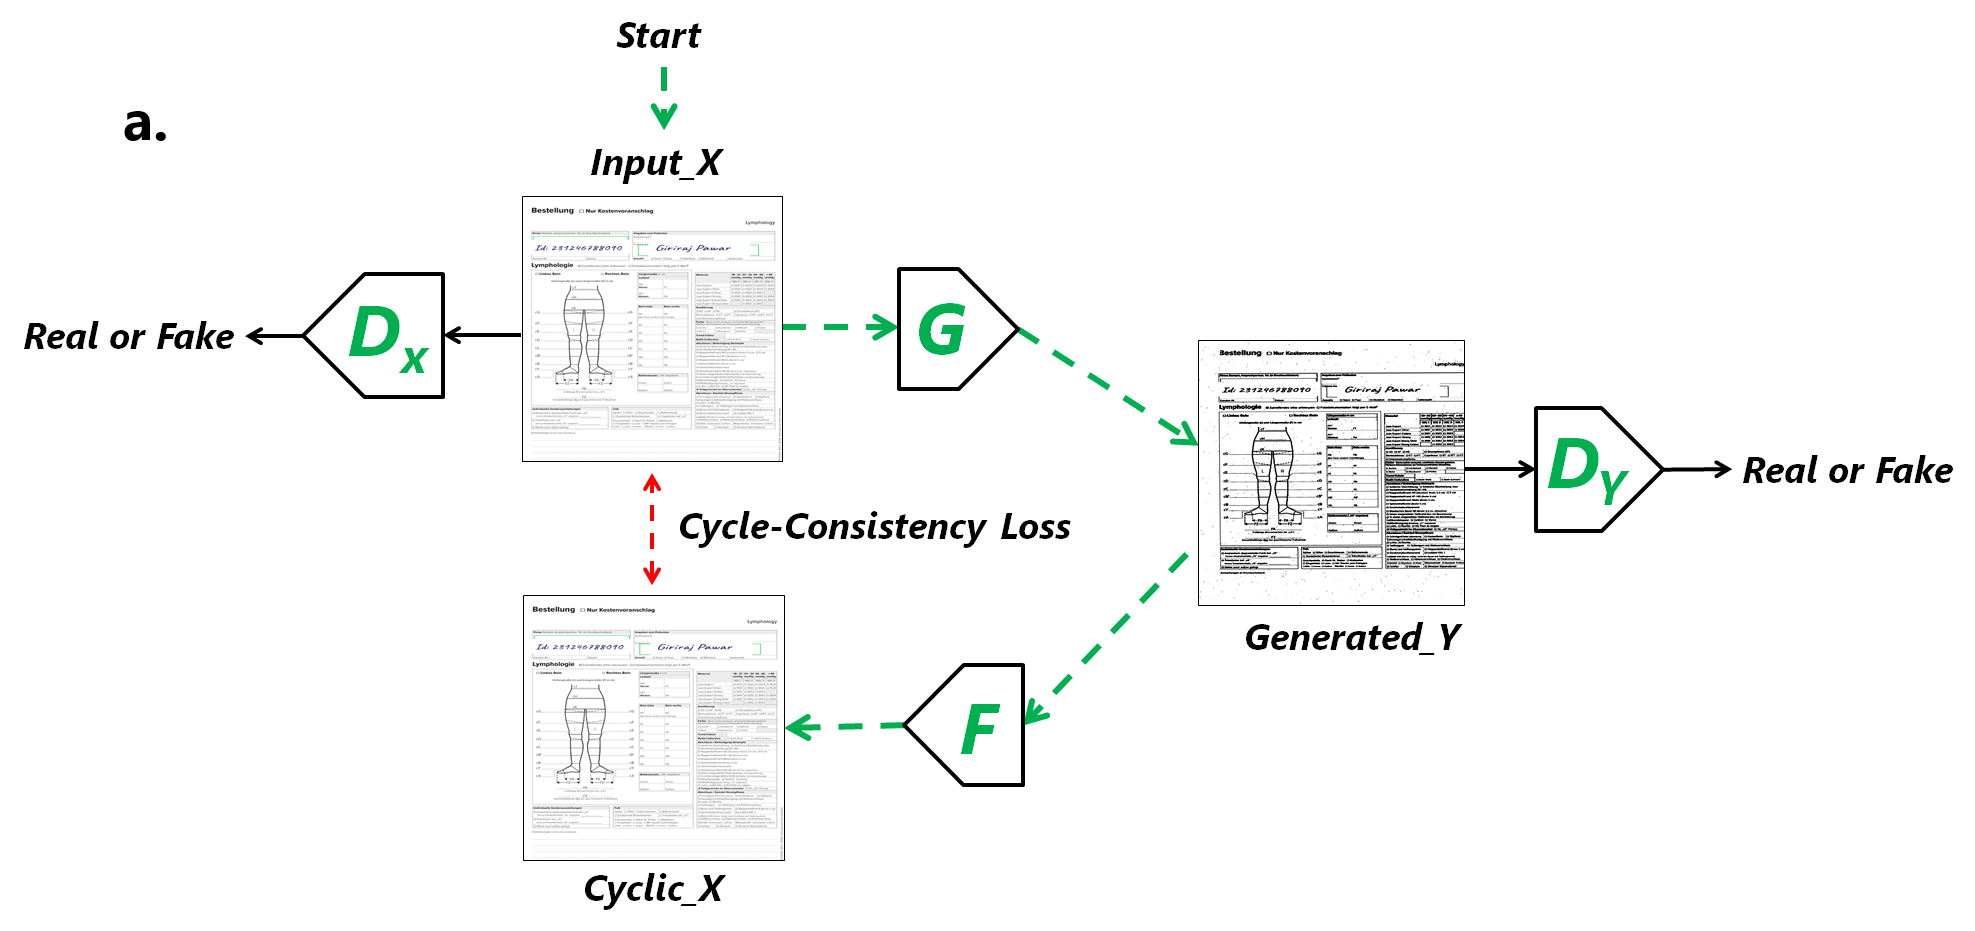
\includegraphics[width=\textwidth]{images/Methodology/Gxy.png}
  \end{minipage}
  \vfill
  \begin{minipage}[b]{0.98\textwidth}
    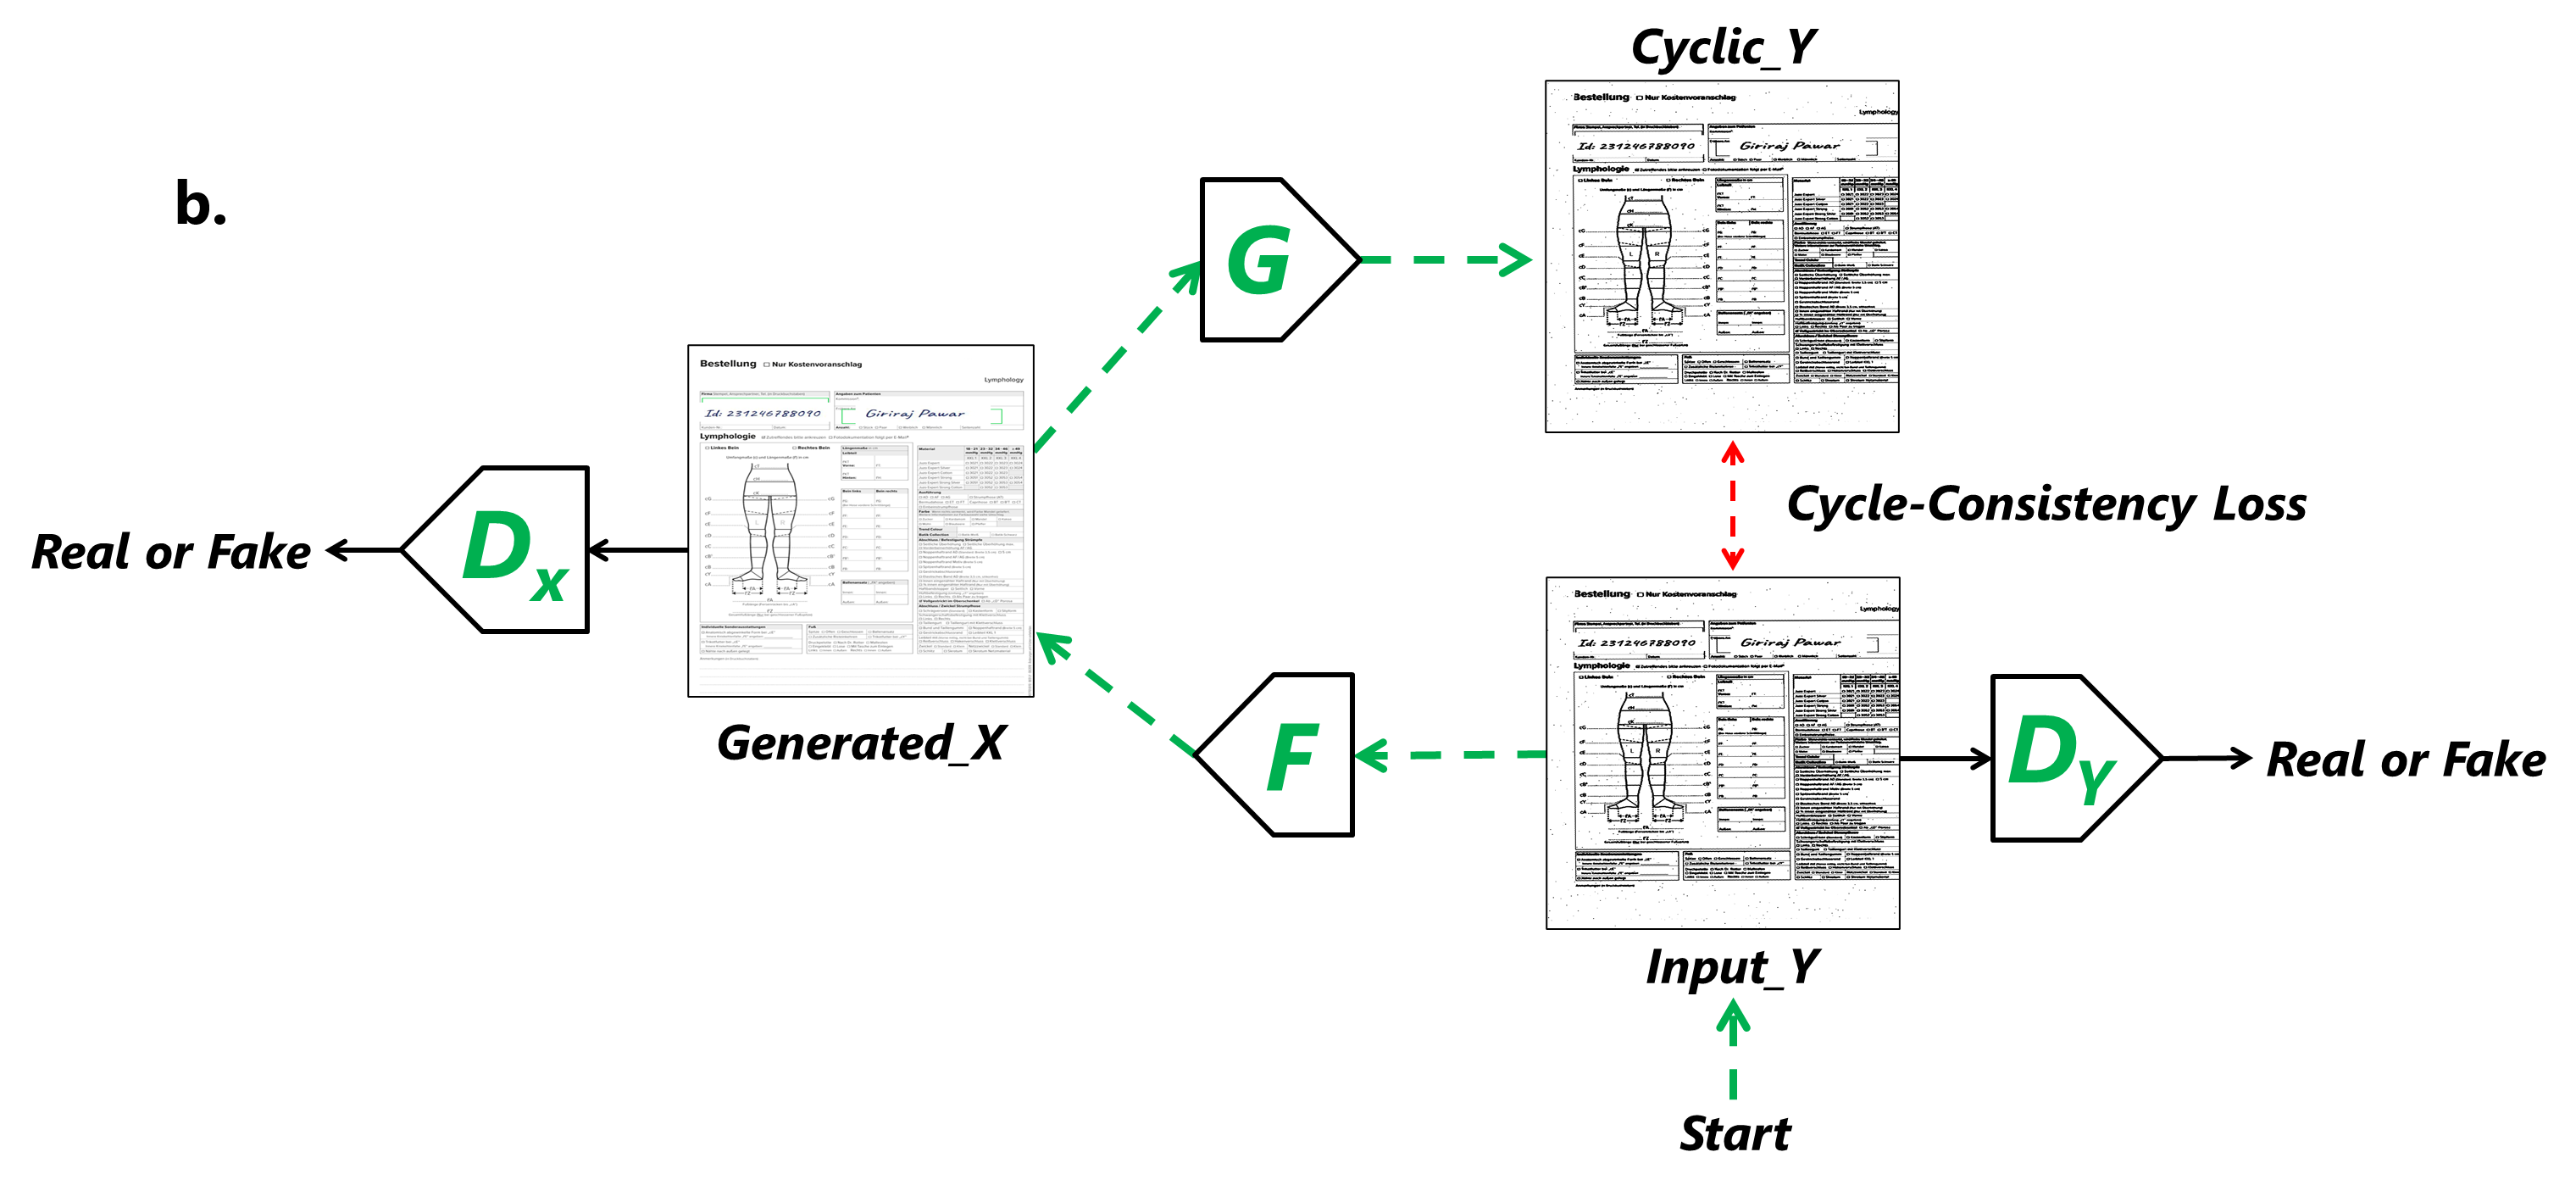
\includegraphics[width=\textwidth]{images/Methodology/Fyx.png}
  \end{minipage}
  \caption[An illustration of the proposed image-to-image translation application using \ac{CycleGAN}, for transforming synthetic document images into real document images and vice versa.]{An illustration of the proposed image-to-image translation application using \ac{CycleGAN}, for transforming synthetic document images into real document images and vice versa. It consists of two generators, $G$ and $F$ which map synthetic document images to real document images and real document images to synthetic document images, respectively, minimizing cycle-consistency loss \cite{zhu2020unpaired}. It also contains two discriminators $D_X$ and $D_Y$ which acts as the adversary and reject images generated by respective generators \cite{zhu2020unpaired}.}
  \label{fig:GxyFyx}
\end{figure}


\section{Cycle-Consistent Adversarial Networks}\label{CycleConsistentAdversarialNetworks}

In \ac{CycleGAN}, the aim is to learn the mapping functions between two domains $X$ and $Y$. The collection of synthetic document images represents source domain $X$ and the collection of real document images represents target domain $Y$. For a given training samples $\{x_i\}_{i=1}^{N}$ where $x_i \in X$ and $\{y_j\}_{j=1}^{M}$ where $y_j \in Y$, the synthetic data distribution represented as $x \sim p_{data}(x)$ and real data distribution represented as $y \sim p_{data}(y)$ \cite{zhao2021unpaired}. The model includes two mappings functions $G : X \rightarrow Y$ and $F : Y \rightarrow X$ as illustrated in figure \ref{fig:GxyFyx}, both are the generators. Along with generators, two adversarial discriminators $D_X$ and $D_Y$ are introduced. $D_X$ learns to distinguish images $\{x\}$ from translated images $\{F(y)\}$. In the same way, $D_Y$ learns to distinguish images $\{y\}$ from $\{G(x)\}$.

The architecture of the \ac{CycleGAN} is illustrated in figure \ref{fig:GxyFyx}. Figure (a) depicts the flow of transformation from synthetic document images to real document images. Figure (b) depicts the flow of transformation from real document images to synthetic document images. It depicts \ac{CycleGAN} has two generators $G$ and $F$, two discriminators $D_X$ and $D_Y$. The discriminator $D_Y$ takes input \textit{Input\_Y} from the target domain $Y$ and fake image \textit{Generated\_Y} generated by the generator $G$. The discriminator $D_Y$ learns to distinguish target domain images from the fake images generated by the $G$ and penalizes itself in the event of misclassification. When the discriminator $D_Y$ determines the image generated by the generator $G$ is fake. It gives feedback to generator $G$ through backpropagation to update its weights to produce good quality images. Next, to achieve cycle-consistency the fake image \textit{Generated\_Y} passed thorough generator $F$ to produce image \textit{Cyclic\_X} back in the source domain $X$ and the cycle-consistency loss is minimized between \textit{Input\_X} and \textit{Cyclic\_X}. 

The discriminator $D_X$ takes input \textit{Input\_X} from the source domain $X$ and fake image \textit{Generated\_X} generated by the generator $F$. The discriminator $D_X$ learns to distinguish source domain images from fake images generated by the generator $F$ and penalizes itself in the event of misclassification. When the discriminator $D_X$ determines the image generated by generator $F$ is fake. It gives feedback to generator $F$ through backpropagation to update its weights to produce good quality images. Next, to achieve cycle-consistency the fake image \textit{Generated\_X} passed thorough generator $G$ to produce image \textit{Cyclic\_Y} back in the target domain $Y$ and the cycle-consistency loss is minimized between \textit{Input\_Y} and \textit{Cyclic\_Y}. The transformation flow of synthetic document images into real document images and vice versa (marked in green dotted arrows) by minimizing the cycle-consistency loss (marked in red dotted arrows) between the input image and cyclically generated image. 


%\subsection{Formulation}
%The least-square loss \cite{mao2017squares} is used for matching the distribution of generated images to the training data distribution.
%In this thesis generators and discriminators used in \ac{CycleGAN} are optimized using least-square loss \cite{mao2017squares} which is opted from \acp{LSGAN}.
%The third is identity mapping loss to preserve the color of the input images \cite{zhu2020unpaired}.
%The general \acp{GAN} uses sigmoid cross-entropy loss function to optimize generator and discriminator. 



\subsection{Cycle-Consistency Loss}\label{CycleConsistencyLoss}

\begin{figure}[H]
	    \begin{center} 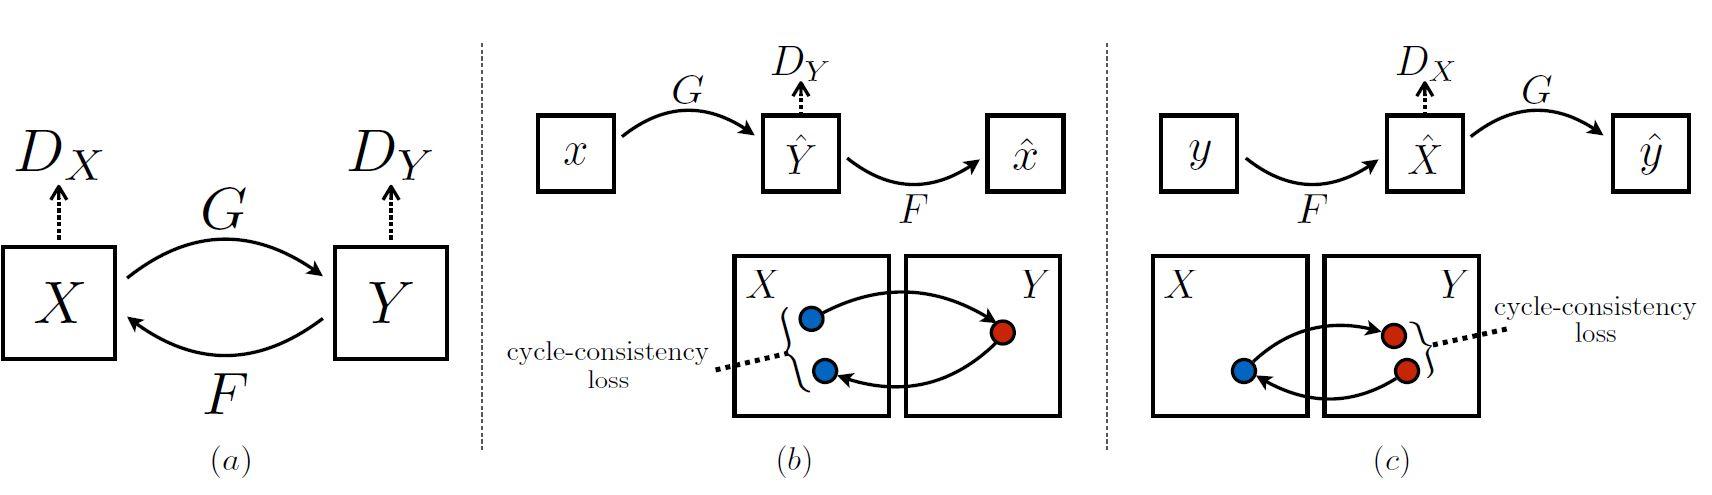
\includegraphics[scale=0.5]{images/Methodology/CycleGAN.jpg}
	    \caption[An illustration of \ac{CycleGAN} model with its mapping functions $G$ and $F$, and respective discriminators $D_Y$ and $D_X$ with depiction forward and backward cycle-consistency loss.]{An illustration of \ac{CycleGAN} model with its mapping functions $G$ and $F$, and respective discriminators $D_Y$ and $D_X$ with depiction forward and backward cycle-consistency loss. (a) \ac{CycleGAN} model with two mapping functions $G : X \rightarrow Y$ and $F : Y \rightarrow X$, and the respective adversarial discriminators are $D_Y$ and $D_X$. (b) for each image $x$ from source domain $X$, the cyclic image-to-image translation brings $x$ back to the original image, i.e., $x \rightarrow G(x) \rightarrow F(G(x)) \approx x$, this is called forward cycle-consistency loss \cite{zhu2020unpaired}. (c) for each image $y$ from target domain $Y$, the cyclic image-to-image translation brings $y$ back to the original image, i.e., $y \rightarrow F(y) \rightarrow G(F(y)) \approx y$, this is called backward cycle-consistency loss \cite{zhu2020unpaired}.}
	    \label{fig:CycleGAN}
	    \end{center}
\end{figure}


The cycle-consistency loss function is the basis of \ac{CycleGAN}. Theoretically, adversarial training can learn mappings that produce outputs identically distributed as target domains $Y$ and $X$, respectively \cite{goodfellow2017nips}. ``However, with a large amount of capacity, a neural network maps the same set of input images to any random permutations of images in the target domain, where any of the learned mappings can produce an output distribution that matches the target distribution'' \cite{goodfellow2017nips}. Hence, depending just on adversarial losses alone cannot promise that the learned mapping function can map an individual input from the source domain $x_i$ to a desired output $y_j$ in the target domain \cite{goodfellow2017nips}. ``To further narrow down and reduce the space of possible outcomes using mapping functions, attempt has been made to argue that learned mapping functions should be cycle-consistent'' \cite{zhu2020unpaired}. The property cycle-consistency can be understood by an example of sentence translation in different language. For example, if an English sentence is translated into German and later from German to English, the outcome should be an original English sentence from where we have started \cite{goodfellow2017nips}. The cycle-consistency loss in the form of a mathematical equation:

\begin{equation}\label{CycleConsistencyLossEquation}
    \mathcal{L}_{cyc}(G, F) = \mathbb{E}_{x \sim p_{data}(x)} (F(G(x)) - x) + \mathbb{E}_{y \sim p_{data}(y)} (G(F(y)) - y).
\end{equation}


\subsection{Least-Square Loss}

In general \acp{GAN} the discriminator is a binary classifier that adopts the sigmoid cross-entropy loss function. As discussed in chapter \ref{relatedworks}, while updating the generator, the sigmoid cross-entropy loss function causes the vanishing gradients problem for the samples that are on the correct side of the decision boundary but are still far from the real data \cite{mao2017squares}.  Also, the sigmoid cross-entropy loss function causes difficulty to stabilize the model training procedure \cite{mao2017squares}. First, $\mathcal{L}_{GAN}$ (equation \ref{ganObjectiveFunction}), the negative log-likelihood objective replaced by a least-squares loss functions \cite{mao2017squares}. The least-squares loss is more stable during training and generates higher quality results \cite{mao2017squares}. It is used to optimize the generator and discriminator adversarially. In the below equations, $a$, $b$ and $c$ are the coding scheme for the equations of the discriminator. Where $a$ and $b$ are the labels for fake data and real data, respectively. $c$ denotes the value that $G$ wants $D$ to believe for fake data. Basically, $a = 0$, $b = 1$ and $c = 1$. That means fake data is represented by $0$ and real data is represented by $1$. Then the improved objective functions using least-squares loss can be defined as follows:

    \begin{equation}\label{lsgan1}
        \underset{D}{\min}\ \mathcal{L}_{ls}(D_Y) = \frac{1}{2}\ \mathbb{E}_{y \sim p_{data}(y)}\ (D_Y(y) - b)^2 + 
        \frac{1}{2}\ \mathbb{E}_{x \sim p_{data}(x)}\ (D_Y(G(x)) - a)^2
    \end{equation}
    
    \begin{equation}\label{lsgan2}
        \underset{G}{\min}\ \mathcal{L}_{ls}(G) = \mathbb{E}_{x \sim p_{data}(x)}\ (D_Y(G(x)) - c)^2]
    \end{equation}
    
    \begin{equation}\label{lsgan3}
    \mathcal{L}_{ls}(G, D_Y, X, Y) =  \underset{D}{\min}\ \mathcal{L}_{ls}(D_Y) + \underset{G}{\min}\ \mathcal{L}_{ls}(G)
    \end{equation}
    
    \begin{equation}\label{lsgan4}
        \underset{D}{\min}\ \mathcal{L}_{ls}(D_X) = \frac{1}{2}\ \mathbb{E}_{x \sim p_{data}(x)}\ (D_X(x) - b)^2 + 
        \frac{1}{2}\ \mathbb{E}_{y \sim p_{data}(y)}\ (D_X(F(y)) - a)^2
    \end{equation}
    
    \begin{equation}\label{lsgan5}        
        \underset{F}{\min}\ \mathcal{L}_{ls}(F) = \mathbb{E}_{y \sim p_{data}(y)}\ (D_X(F(y)) - c)^2
    \end{equation}
    
    
    \begin{equation}\label{lsgan6}        
        \mathcal{L}_{ls}(F, D_X, Y, X) = \underset{D}{\min}\ \mathcal{L}_{ls}(D_X) + \underset{F}{\min}\ \mathcal{L}_{ls}(F)
    \end{equation}
    



%\ref{CycleConsistencyLossEquation}.
%$G$ and $F$ both should satisfy cycle-consistency.
	    


\subsection{Identity Mapping Loss}

The identity mapping loss encourages the mapping to preserve color composition between the input and output \cite{taigman2016unsupervised}. As described earlier, generator $G$ transforms synthetic document images into realistic document images. The identity mapping loss regularizes the generator $G$ to produce samples identical to the real document images when real samples are provided as an input. It is similar with the generator $F$, but vice versa, the identity mapping loss regularizes it to produce samples identical to the synthetic document images when synthetic samples are provided as an input. It means providing an input to the generator from the same domain in which it is transforming into, the output should be identical to the given input. The identity mapping loss in the form of a mathematical equation:

\begin{equation}\label{IdentityMappingLoss}
    \mathcal{L}_{ide}(G, F) = \mathbb{E}_{y \sim p_{data}(y)}(F(y) - y) + \mathbb{E}_{x \sim p_{data}(x)}(G(x) - x).
    \end{equation}

\subsection{Complete Objective Function}

Combining equations \ref{lsgan6}, \ref{CycleConsistencyLossEquation} and \ref{IdentityMappingLoss} the final objective is achieved. The model is optimized using least-squares loss, cycle-consistency loss and identity mapping loss. In equation \ref{FullObjective}, the terms $\lambda_{cyc}$ and $\lambda_{identity}$ control the relative importance of the term in the objective. The complete objective function in the form of a mathematical equation:

\begin{equation}\label{FullObjective}
\begin{aligned}
    \mathcal{L}(G, F, D_X, D_Y) =  \mathcal{L}_{ls}(G, D_Y, X, Y)\ +\ \mathcal{L}_{ls}(F, D_X, Y, X)\ +\ 
    \lambda_{ide}\ \mathcal{L}_{ide}(G, F)\ +\ \lambda_{cyc}\ \mathcal{L}_{cyc}(G, F).
\end{aligned}
\end{equation}
    

\section{\ac{CycleGAN} Training Algorithm}\label{CycleGANAlgorithm}

%Below, the algorithm of the \ac{CycleGAN} is described in the form of pseudo-code. The pseudo-code could be understood clearly by referring to figure \ref{fig:GxyFyx}.


\begin{algorithm}[H]
\For{each training iteration}{
 \BlankLine
	Draw a random sample $x_i$ from source domain $X$ where $\{x_i\}_{i=1}^{N}$  and $x_i \in X$ \\
	\BlankLine
	Draw a random sample $y_j$ from target domain $Y$  where $\{y_j\}_{j=1}^{M}$ and $y_j \in Y$ \\
	\BlankLine
	\textbf{1. Train the Discriminators:}\\
	\BlankLine
	\BlankLine
	\Indp
		a) Compute the discriminator loss on real and fake images:\\
		\BlankLine
		\Indp
		    	$\mathcal{L}_{real,fake}^{(D_X)} = \frac{1}{2}\ (D_X(x_i) - 1)^2 + \frac{1}{2}\ (D_X(F(y_j)))^2$\\
		\BlankLine
		\BlankLine
			$\mathcal{L}_{real,fake}^{(D_Y)} = \frac{1}{2}\ (D_Y(y_j) - 1)^2 + \frac{1}{2}\ (D_Y(G(x_i)))^2$\\
		\BlankLine
		\Indm

		c) Update the discriminators\\
	\Indm
	
	\BlankLine
	\BlankLine
	\BlankLine
	
	\textbf{2. Train the Generators:}\\
	\BlankLine
	\BlankLine
	\Indp
		a) Compute the cycle-consistency losses:\\
		\BlankLine
		\Indp
			$\mathcal{L}_{cyc}^{(X \rightarrow Y \rightarrow X)} = F(G(x_i)) - x_i$\\
			\BlankLine
			$\mathcal{L}_{cyc}^{(Y \rightarrow X \rightarrow Y)} = G(F(y_j)) - y_j$\\
			\BlankLine
		\Indm
		b) Compute the identity mapping losses:\\
		\BlankLine
		\Indp
			\BlankLine	
			$\mathcal{L}_{ide}^{(X \rightarrow X)} = G(x_i) - x_i$\\
			\BlankLine
			$\mathcal{L}_{ide}^{(Y \rightarrow Y)} = F(y_j) - y_j$\\
			\BlankLine			
		\Indm
		c) Compute the Generator $G$ loss:\\
		\Indp
			\BlankLine	
			$\mathcal{L}_{G} = (D_Y(G(x_i)) - 1)^2 + \mathcal{L}_{cyc}^{(Y \rightarrow X \rightarrow Y)} + \mathcal{L}_{ide}^{(Y \rightarrow Y)}$\\
			\BlankLine	
			Compute the Generator $F$ loss:\\
			\BlankLine	
			$\mathcal{L}_{F} = (D_X(F(y_j)) - 1)^2 + \mathcal{L}_{cyc}^{(X \rightarrow Y \rightarrow X)} + \mathcal{L}_{ide}^{(X \rightarrow X)}$\\
			\BlankLine
		\Indm
		d) Update the generators\\
	\Indm	
	\BlankLine
}	


\caption{\ac{CycleGAN} training algorithm.}
\label{alg:CycleGANAlgorithm}
\end{algorithm}





















































%%%%%%%%%%%%%%%%%%%%%%%%%%%%%%%%%%%%%%%%%%%%%%%%%%%%%%%%%%%%%%%%%%%%%%%%%%%%%%%%%%%%%%%%%%%%%%%%%%%%%%%%%%%%%%%%%5

%Adversarial training can, in theory, learn mappings $G$ and $F$ that produce outputs identically distributed as target domains $Y$ and $X$ respectively. However, with large enough capacity, a network can map the same set of input images to any random permutation of images in the target domain, where any of the learned mappings can induce an output distribution that matches the target distribution. Thus, adversarial losses alone cannot guarantee that the learned function can map an individual input $x_i$ to a desired output $y_i$. To further reduce the space of possible mapping functions, we argue that the learned mapping functions should be cycle-consistent: 

%The aim is to learn mapping functions between two domains $X$ and $Y$. The Domain $X$ represents synthetic document images distribution and domain $Y$ represents real document images distribution. Given training samples $\{x_i\}_{i=1}^{N}$ where $x_i \in X$ and  $\{y_j\}_{j=1}^{M}$ where $y_j \in Y$. We denote the data distribution $x \sim p_{data}(x)$  and $y \sim p_{data}(y)$.

\begin{comment}
\subsection{Adversarial Loss}
We apply adversarial losses \cite{goodfellow2014generative} to both mapping functions. For the mapping function $G : X \rightarrow Y$  and its discriminator $D_Y$ , we express the objective as:

    \begin{equation}\label{AdversarialLoss}
    \mathcal{L}_{GAN}(G, D_Y, X, Y) = \mathbb{E}_{y \sim p_{data}(y)} [\log D_Y(y)] + \mathbb{E}_{x \sim p_{data}(x)}[\log (1 - D_Y(G(x)))],
    \end{equation}
    
where $G$ tries to generate images $G(x)$ that look similar to images from domain $Y$ , while $D_Y$ aims to distinguish between translated samples $G(x)$ and real samples $y$. $G$ aims to minimize this objective against an adversary $D$ that tries
to maximize it, i.e., $\min_{G} \max_{D_Y} \mathcal{L}_{GAN}(G, D_Y, X, Y)$. We introduce a similar adversarial loss for the mapping function $F : Y \rightarrow X$ and its discriminator $D_X$ as well: i.e., $\min_{F} \max_{D_X} \mathcal{L}_{GAN}(F, D_X, Y, X)$.

\end{comment}

\begin{comment}
We aim to solve:
\begin{equation}\label{FullObjectiveAimToSolve}
    G^*, F^* = \arg\underset{G, F}{\min}\underset{D_X, D_Y}{\min} \mathcal{L}(G, F, D_X, D_Y)
    \end{equation}
\end{comment}


\begin{comment}
\begin{figure}[H]
        \begin{center}
    	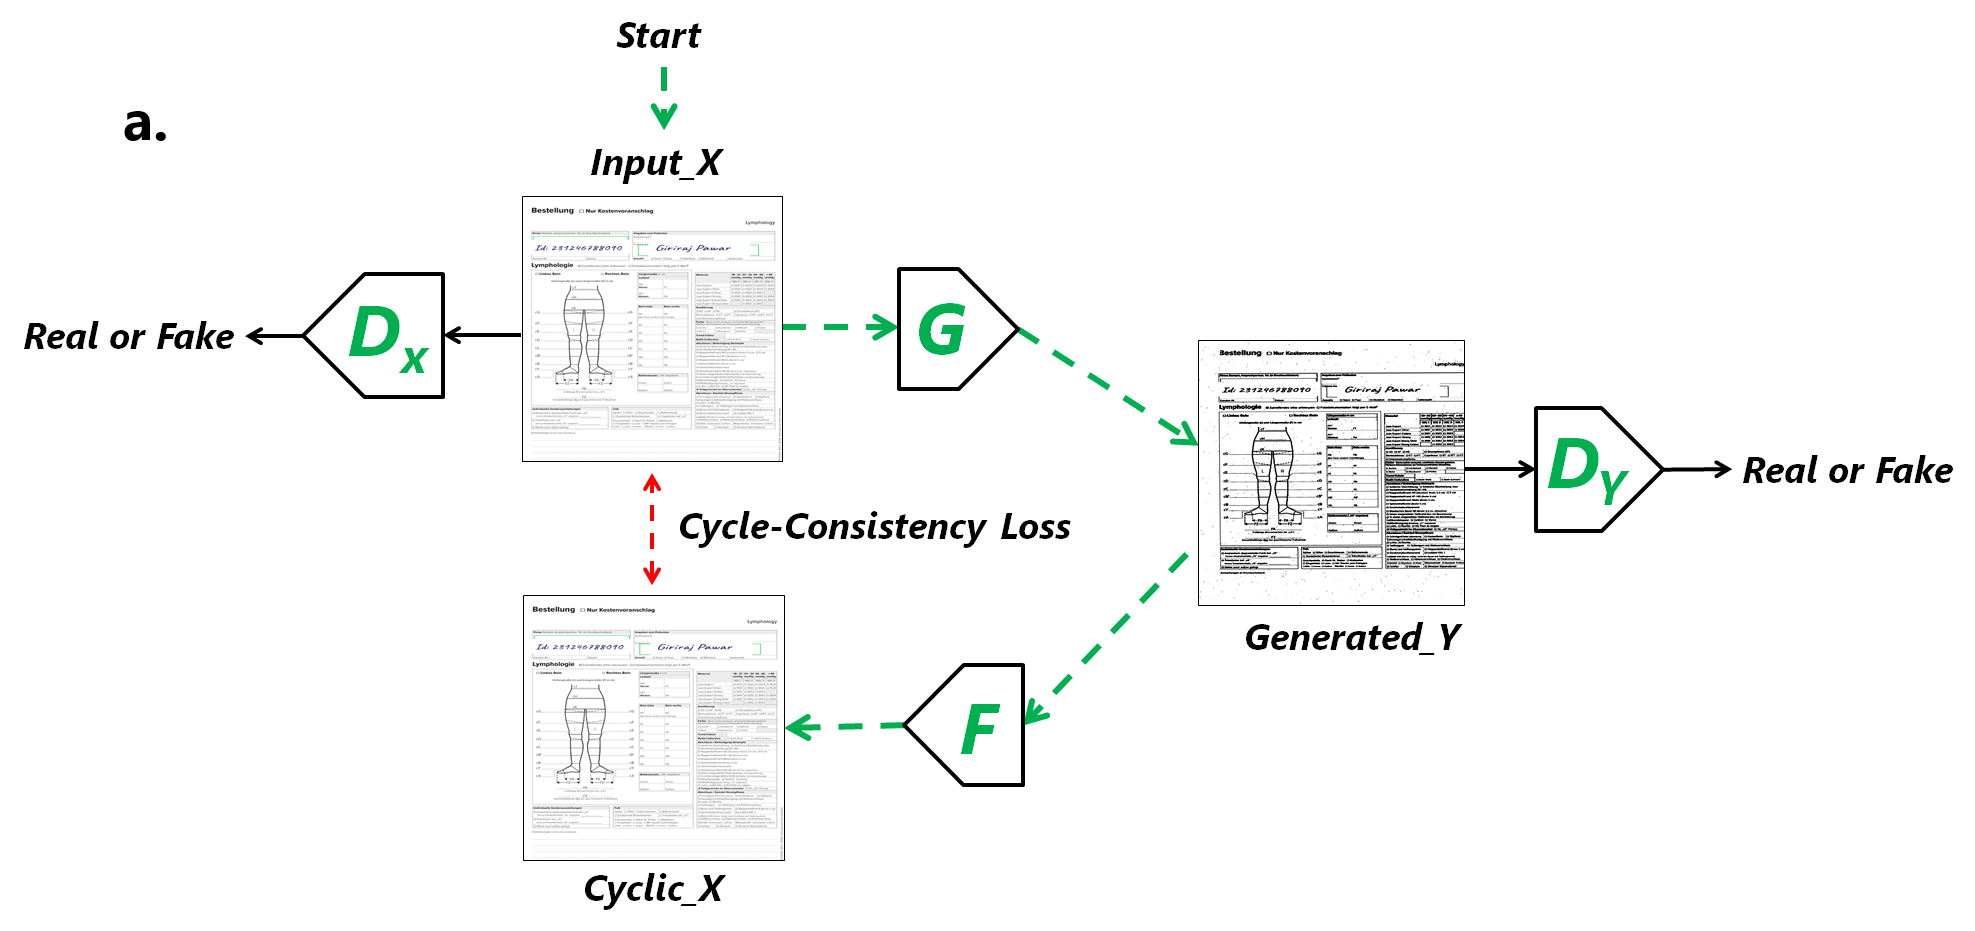
\includegraphics[scale=0.20]{images/Methodology/Gxy.png}
	    \caption[The transformation flow of synthetic document images into realistic document images using generator $G$.]{The transformation flow of synthetic document images into realistic document images using generator $G$. The transformation flow is marked by green dotted arrows. The generator $G$ is a mapping function $G: X \rightarrow Y$ which transforms images from the source domain to the target domain by minimizing the cycle-consistency loss (red dotted arrow) between the input image and cyclically generated image.}
	    \label{fig:Gxy}
	    \end{center}
\end{figure}

\begin{figure}[H]
        \begin{center}
    	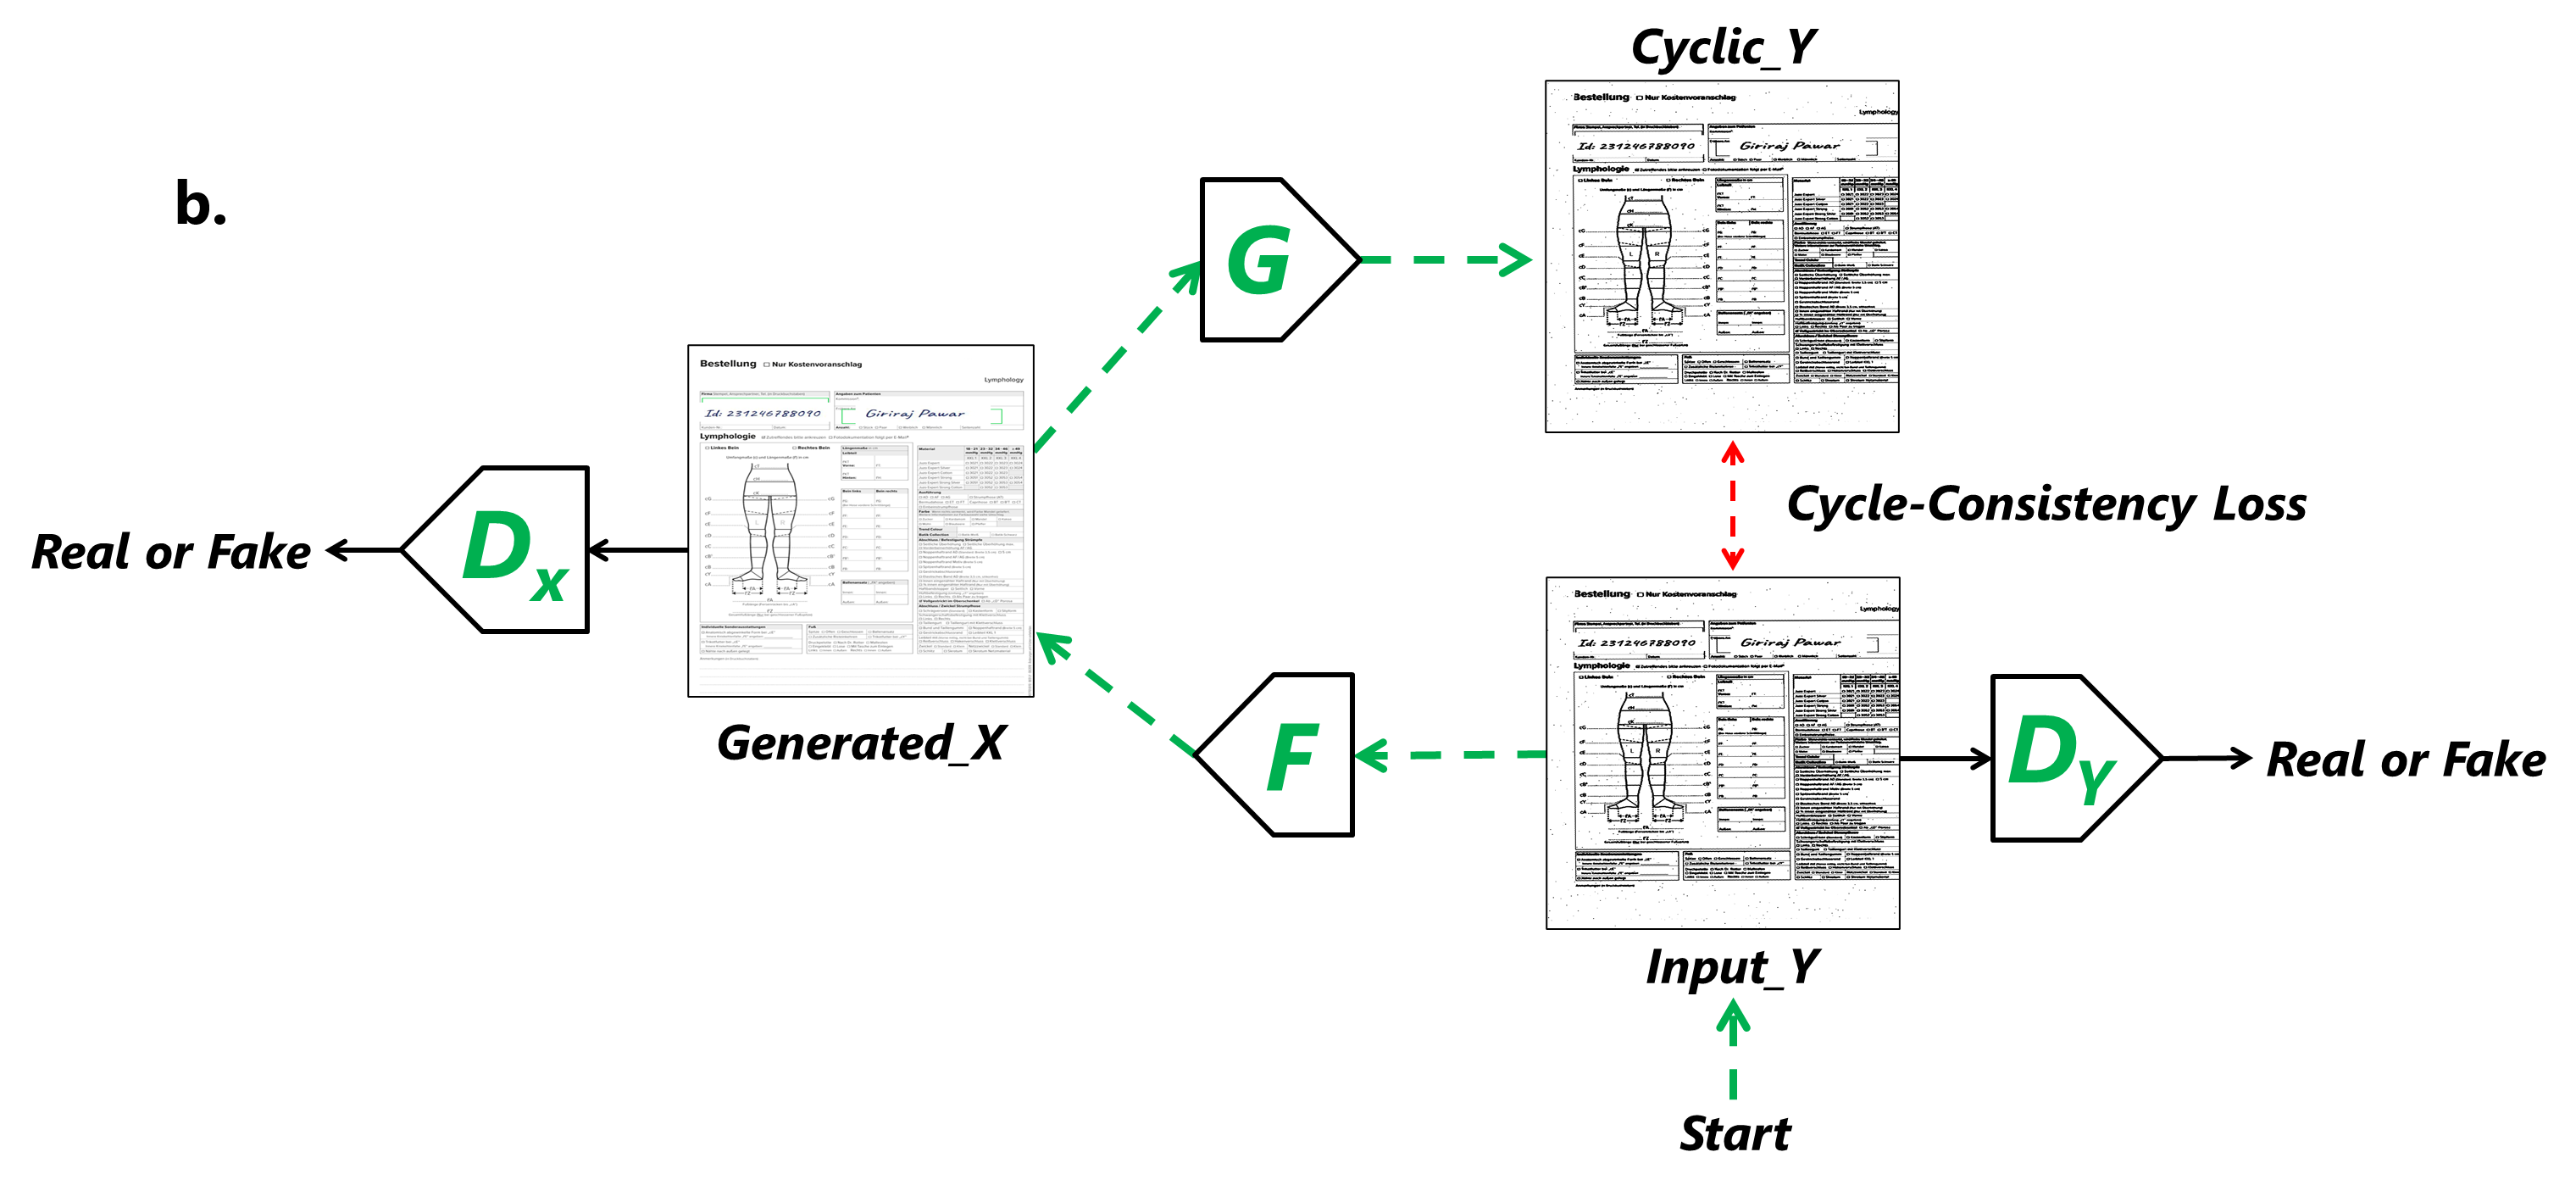
\includegraphics[scale=0.20]{images/Methodology/Fyx.png}
	    \caption[The transformation flow of real document images into synthetic document images using generator $F$.]{The transformation flow of real document images into synthetic document images using generator $F$. The transformation flow is marked in green dotted arrows. The generator $F$ is mapping function $F: Y \rightarrow X$ which transforms images from the target domain to the source domain by minimizing the cycle-consistency loss (red dotted arrow) between the input image and cyclically generated image.}
	    \label{fig:Fyx}
	    \end{center}
\end{figure}


%It is helpful to introduce an additional loss to encourage the mapping to preserve color composition between the input and output. In particular, we adopt the technique of \cite{taigman2016unsupervised} and regularize the generator to be near an identity mapping when real samples of the target domain are provided as the input to the generator

%Below, the algorithm of the \ac{CycleGAN} is described in the form of pseudo-code. The pseudo-code could be understood clearly by referring to figure \ref{fig:GxyFyx}.



\begin{algorithm}[H][1]
\For{each training iteration}{
 \BlankLine
 \BlankLine
 \BlankLine
 \textbf{1. Train the Generators:}
	\BlankLine
	\BlankLine
	\Indp
	1. Get a random image \textit{Input\_X} from source domain $X$ from the training dataset.\\
	2. Get a random image \textit{Input\_Y} from target domain $Y$ from the training dataset. \\
	\BlankLine
 	\BlankLine
	3. Pass \textit{Input\_X} through generator $G$ and generate fake image \textit{Generated\_Y}.\\
	4. Pass \textit{Input\_Y} through generator $F$ and generate fake image \textit{Generated\_X}.\\
	\BlankLine
 	\BlankLine
	5. Pass \textit{Generated\_Y} through generator $F$ and generate cyclic image \textit{Cyclic\_X}.\\
	6. Pass \textit{Generated\_X} through generator $G$ and generate cyclic image\textit{Cyclic\_Y}.\\
	\BlankLine
 	\BlankLine
	7. Pass \textit{Input\_X} through generator $G$ and generate identical image \textit{Same\_X}.\\
	8. Pass \textit{Input\_Y} through generator $F$ and generate identical image \textit{Same\_Y}.\\
	\BlankLine
 	\BlankLine
 \Indm
 \textbf{2. Train the Discriminators:}
	1. Pass \textit{Input\_X} through generator $G$ and generate identical image \textit{Same\_X}.\\
     2. Pass \textit{Input\_Y} through generator $F$ and generate identical image \textit{Same\_Y}.\\
 	\BlankLine
 	\BlankLine
	\Indp
	
\BlankLine
\BlankLine
\BlankLine
}	
	\caption{CycleGAN training algorithm.}
\label{alg:CycleGANAlgorithm}
\end{algorithm}





\end{comment}


\newpage

\chapter{Implementation}
    \label{implementation}
    %\noindent
\justifying
\setlength{\parskip}{1em}

This chapter discusses the implementation of the \ac{CycleGAN} and Classifiers. In this thesis, classifiers are used to determine the domain gap between the distributions. Also, they are used to evaluate the quality of images generated by the \ac{CycleGAN}. How the classifiers are being used to analyze the domain gap between distributions will be discussed in-depth in chapter Evaluation \ref{evaluation}. In section \ref{DatasetPreparation} dataset preparation is described. The architecture of \ac{CycleGAN} and Classifiers discussed in section \ref{NetworkArchitecture}. The training details of \ac{CycleGAN} and Classifiers described in \ref{TrainingDetails}. The experiments are visualized using Tensorboard\footnotemark. TensorBoard is a tool that provides the visualization needed for machine learning research and experiments. The neural networks implemented in this thesis using Python, Keras APIs, and TensorFlow library\cite{tensorflow2015-whitepaper}. The reference code for the \ac{CycleGAN} is available \href{https://keras.io/examples/generative/cyclegan/}{here}. All of the neural networks are trained upon GPUs (Graphics Processing Units) like Nvidia Tesla T4 and Tesla V100-SXM2.

\footnotetext{\url{https://www.tensorflow.org/tensorboard} last access: 22.07.2021}


\section{Dataset Preparation}\label{DatasetPreparation}

\begin{figure}[H]
        \begin{center}
    	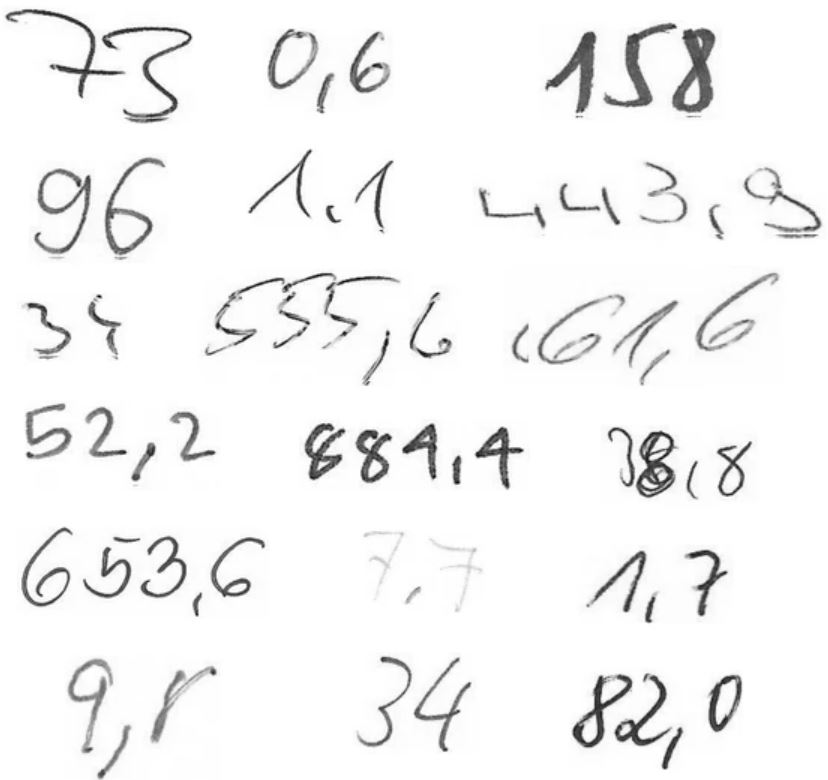
\includegraphics[scale=0.45]{images/keinwifi.JPG}
	    \caption[Examples of handwritting crops from the handwritting number dataset.]{Examples of handwritting crops from the handwritting number dataset. (Figure reproduced from elevait GmbH \& Co. KG with permission.)}
	    \label{fig:keinwifi}
	    \end{center}
\end{figure}


The dataset preparation is one of the vital aspects of training any neural network. Bad quality data leads to a poor generalization of neural networks. There are ten types of documents that were considered to work with this image-to-image translation application. Hence, the \ac{CycleGAN} is trained using a stash of synthetic document images and real document images. Around 100,000 synthetic document images in the source domain and the same number of real document images in the target domain. The synthetic document images are generated using unfilled form image (figure \ref{fig:EmptyForm}) and handwritten crops (figure \ref{fig:keinwifi}). The process of inserting handwritten crops on empty templates can be visualized in figure \ref{fig:InsertHandwrittenCrops}. Each unfilled form image is filled with the help of provided bounding box annotations \cite{lin2015microsoft}. For each class of unfilled form image 10,000, synthetic document images are created. As mentioned earlier, 100,000 synthetic document images are created in total. The same created 100,000 synthetic document images are used while training \ac{CycleGAN}. Just they are stashed at the same location collectively. The created 100,000 synthetic document images were also faxified and a faxified dataset of 100,000 images is created. It has the same structure as synthetic document images, 10 classes, and each class has 10,000 images. The faxification process uses several image transformations to make a clean gray-scale image look like it was sent via fax. A sample faxified image can be seen in figure \ref{fig:FaxifiedImage}. The faxification process is described briefly in Section \ref{trainingfaxifiedclassifier}. Also, the faxification can be visualized in figure \ref{fig:FaxificationProcess}. In the table \ref{table:datasets} the number of samples in each dataset is mentioned. For testing, around 1162 annotated real document images are used. This testing dataset is used to evaluate the performance of the classifiers trained upon different data distributions like synthetic document images, faxified document images, and \ac{CycleGAN} generated document images. Basically, testing dataset is significant to understand the domain gap between real data distribution and remaining data distributions. In the table \ref{table:testdataset} the number of samples in each class in the test dataset is mentioned. The testing dataset is unbalanced. The datasets used in this thesis can not be cited or published because they are not open for public use.

\begin{figure}[H]
        \begin{center}
	    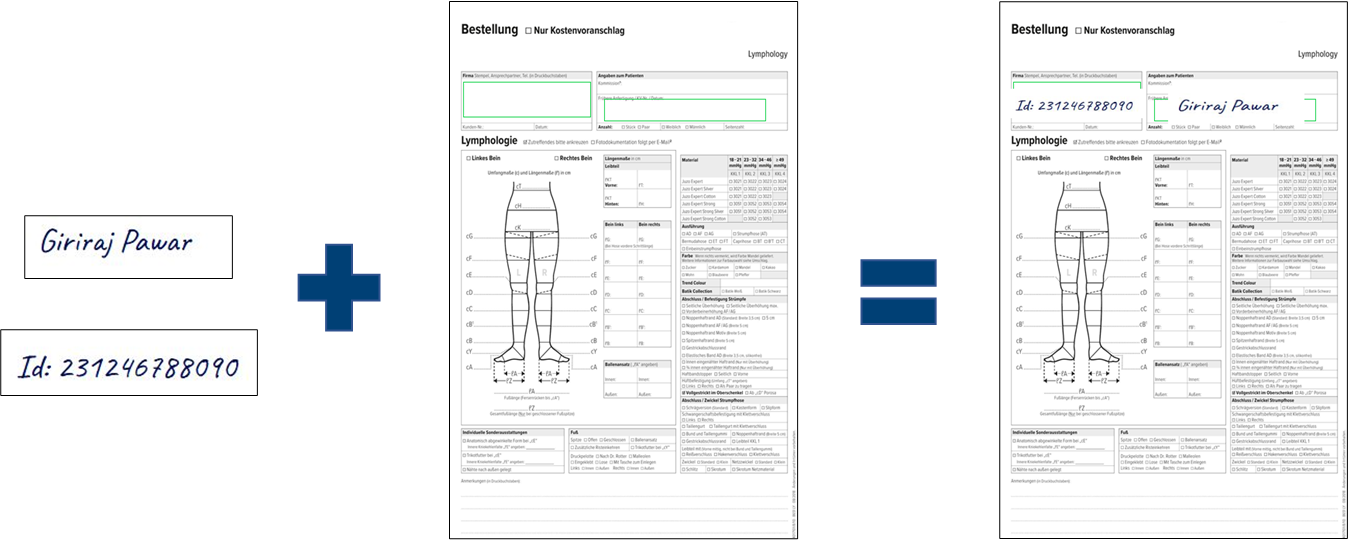
\includegraphics[scale=0.40]{images/InsertHandwrittenCrops.png}
	    \caption[Inserting handwritten crops on empty form templates.]{Inserting handwritten crops on empty form templates.}
	    \label{fig:InsertHandwrittenCrops}
	    \end{center}
\end{figure}


\begin{center}
    \begin{table}[H]
    \begin{center}
    \begin{tabular}{||c c||} 
    \hline
    \textbf{Datasets} & \textbf{Size (Number of Images)}\\ [0.5ex] 
    \hline\hline
    Synthetic Document Images & 100,000 \\ 
    \hline
    Real Document Images & 100,000 \\
    \hline
    Faxified Document Images & 100,000 \\
    \hline
    Annotated Real Document Images (Used for testing) & 1162 \\
    \hline
    \end{tabular}
    \end{center}
    \caption{Size of Datasets used for training \ac{CycleGAN} and Classifiers.}
    \label{table:datasets}
    \end{table}
\end{center}

\begin{center}
    \begin{table}[H]
    \begin{center}
    \begin{tabular}{||c c||} 
    \hline
    \textbf{Classes} & \textbf{Size (Number of Images)}\\ [0.5ex] 
    \hline\hline
    DE\_LY\_Arm\_2020-01 & 44 \\ 
    \hline
    DE\_LY\_Bein\_2018-08 & 47 \\
    \hline
    DE\_LY\_Bein\_2019-01 & 50 \\
    \hline
    DE\_LY\_Bein\_2019-07&  60\\
    \hline
    DE\_LY\_Bein\_2020-01&  624\\
    \hline
    DE\_LY\_Bein\_2020-03&  128\\
    \hline
    DE\_LY\_Hand\_2020-01&  16\\
    \hline
    DE\_PH\_Bein\_2018-09&  22\\
    \hline
    DE\_PH\_Bein\_2019-02&  28\\
    \hline    
    DE\_PH\_Bein\_2020-01&  143\\
    \hline    
    \end{tabular}
    \end{center}
    \caption[Number of Images in each Class of Annotated Real Document Images Dataset.]{Number of Images in each Class of Annotated Real Document Images Dataset (testing dataset).}
    \label{table:testdataset}
    \end{table}
\end{center}


\section{Network Architecture}\label{NetworkArchitecture}

\subsection{\ac{CycleGAN}}

Johnson et al.\cite{johnson2016perceptual} proposed the architecture of \ac{CycleGAN}. In which the generator has three sequences of blocks one is downsampling, transformation, and upsampling. The sequence of 2 downsampling convolutional blocks encode the $256 \times 256 \times 1$ grayscale input image, 9 \ac{ResNet} convolutional blocks to transform the image, and 2 upsampling convolutional blocks to generate the output image of the same dimension as the input image. The reason behind using residual blocks is it resolves the vanishing gradient problem in deep neural networks. The discriminator classifier network is designed using PatchGAN architecture \cite{isola2018imagetoimage} \cite{li2016precomputed}. The PatchGAN discriminator is simply a \ac{CNN}. The major difference between the PatchGAN discriminator and General \ac{GAN} discriminator is, \ac{GAN} discriminator maps input image to the scalar output, which represents image being real to fake. But, the PatchGAN discriminator maps the input image to $N \times N$ array of outputs, where each element in an output array represent a patch in an input image being real or fake. Basically, the PatchGAN discriminator penalizes structure at the scale of local image patches and attempts to classify if each $M \times M$ patch in an image is real or fake.

Johnson et al. \cite{johnson2016perceptual} have provided naming conventions to define the architecture of generator and discriminator used in \ac{CycleGAN}. {\fontfamily{qcr}\selectfont c7s1-k} denotes a $7 \times 7$ Convolution-InstanceNormlization-ReLU layer with $k$ filters and stride 1. The downsampling block {\fontfamily{qcr}\selectfont dk} is denoted by a $3 \times 3$ Convolution-InstanceNormlization-ReLU layer with $k$ filters and stride 2. To reduce artifacts reflection padding is used. {\fontfamily{qcr}\selectfont Rk} denotes a single residual block that has two $3 \times 3$ convolution layers with the same number of filters $k$ on both layers and stride 1. The upsampling block {\fontfamily{qcr}\selectfont uk} denoted a $3 \times 3$ TransposedConvolution-InstanceNormlization-ReLU layer with $k$ filters and stride 2. The complete generator network with 9 residual blocks can be described as: {\fontfamily{qcr}\selectfont c7s1-64, d128, d256, R256, R256, R256, R256, R256, R256, R256, R256, R256, u128, u64, c7s1-1}. The last layer {\fontfamily{qcr}\selectfont c7s1-1} denotes a $7 \times 7$ Convolution layer with 1 filter and stride 1. Next, the final output is followed by a tanh activation function (figure \ref{fig:ActivationFunctions}). All of the layers in the generator can be seen in figure \ref{fig:GeneratorModelSummary}. The architecture of the generator is illustrated in table \ref{table:GeneratorArchitecture}. Also, in the figure \ref{fig:resnetBlock} \ac{ResNet} blocks in the generator network illustrated. In which, at every \ac{ResNet} block, the output from the previous layer is passed through \ac{ResNet} convolution layers. Further, it concatenated with the \ac{ResNet} convolution layer's output and forwarded to the following layers.

\vspace*{1.0cm}
\begin{figure}[H]
        \begin{center}
	    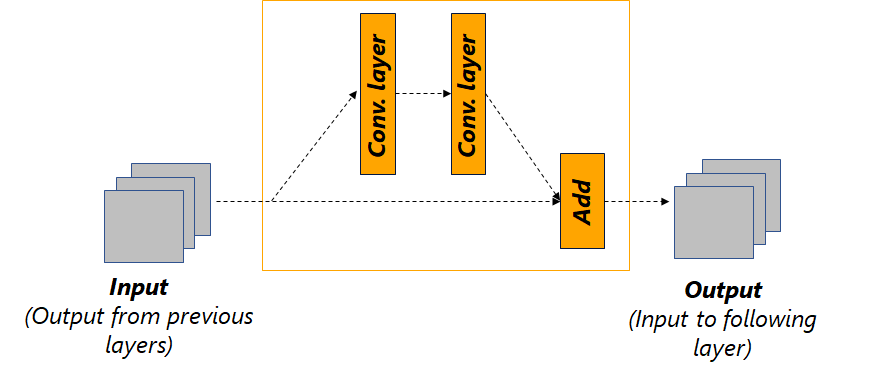
\includegraphics[scale=0.65]{images/Implementation/resnetBlocks.png}
	    \caption[Illustration of ResNet Blocks in \ac{CycleGAN} Generator Architecture.]{Illustration of ResNet Blocks in \ac{CycleGAN} Generator Architecture.}
	    \label{fig:resnetBlock}
	    \end{center}
\end{figure}




\begin{table}[H]
    \centering

    \begin{tabular}{P{0.35\linewidth} P{0.20\linewidth} P{0.20\linewidth} P{0.20\linewidth}} 
        \toprule
        \textbf{Operation Layer} & \textbf{Number of Filters/Units} & \textbf{Size of Each Filter} & \textbf{Stride Value}\\
        \toprule
        \toprule
        Input Image \\($256 \times 256 \times 1$) & - & - & - \\
        \midrule
        Convolution Layer\\Instance Normalization\\ReLU & 64 & $7 \times 7$ & $1 \times 1$\\
        \midrule
        Convolution Layer\\Instance Normalization\\ReLU & 128 & $3 \times 3$ & $2 \times 2$\\
        \midrule
        Convolution Layer\\Instance Normalization\\ReLU & 256 & $3 \times 3$ & $2 \times 2$\\
        \midrule
        \textbf{9 Residual Blocks}\\
	  2 Convolution Layers\\ \textit{(each with)}\\Instance Normalization\\ReLU & 256 & $3 \times 3$ & $1 \times 1$\\
        \midrule
        Transposed Convolution Layer\\Instance Normalization\\ReLU & 128 & $3 \times 3$ & $2 \times 2$\\
        \midrule
        Transposed Convolution Layer\\Instance Normalization\\ReLU & 64 & $3 \times 3$ & $2 \times 2$\\
        \midrule
         Convolution Layer\\tanh & 1 & $7 \times 7$ & $1 \times 1$\\
        \midrule
        \midrule
        Output  \\($256 \times 256 \times 1$) & - & - & -\\
        \bottomrule
    \end{tabular}
    \caption[Generator Architecture]{Generator Architecture}
    \label{table:GeneratorArchitecture}
\end{table}



The discriminator uses $70 \times 70$ PatchGAN classfier architecture \cite{isola2018imagetoimage}. It is also called a Markovian discriminator \cite{li2016precomputed}. The L1 and L2 loss functions produce blurry results while solving
image generation problems \cite{ledig2017photorealistic}. These losses fail to encourage high-frequency crispness. To model high frequencies, more attention is given to the structure in local image patches \cite{isola2018imagetoimage}. Therefore Markovian discriminator is called the PatchGAN discriminator. {\fontfamily{qcr}\selectfont Ck} denotes a $4 \times 4$ Convolution-InstanceNormalization-LeakyReLU layer with $k$ filters and stride 2. Leaky ReLUs with a slope of 0.2 are used. Instance Normalization is not used for the first {\fontfamily{qcr}\selectfont C64} layer. After the last layer {\fontfamily{qcr}\selectfont C512}, the convolution operation is applied with filter 1 to produce an output of depth 1 using $4 \times 4$ kernel and stride 1. The discriminator network can be described as: {\fontfamily{qcr}\selectfont C64-C128-C256-C512-C512-C1}. All of the layers in the discriminator can be seen in figure \ref{fig:DiscriminatorModelSummary}. The architecture of the classifier is illustrated in table \ref{table:DiscriminatorArchitecture}.





\begin{table}[H]
    \centering

    \begin{tabular}{P{0.30\linewidth} P{0.20\linewidth} P{0.20\linewidth} P{0.20\linewidth}} 
        \toprule
        \textbf{Operation Layer} & \textbf{Number of Filters/Units}  & \textbf{Size of Each Filter} & \textbf{Stride Value}\\
        \toprule
        \toprule
        Input Image \\($256 \times 256 \times 1$) & - & - & -\\
        \midrule
        Convolution Layer\\Instance Normalization\\LeakyReLU (0.2) & 64 & $4 \times 4$ & $2 \times 2$\\
        \midrule
        Convolution Layer\\Instance Normalization\\LeakyReLU (0.2) & 128 & $4 \times 4$ & $2 \times 2$\\
        \midrule
        Convolution Layer\\Instance Normalization\\LeakyReLU (0.2) & 256 & $4 \times 4$ & $2 \times 2$\\
        \midrule
        Convolution Layer\\Instance Normalization\\LeakyReLU (0.2) & 512 & $4 \times 4$ & $1 \times 1$\\
        \midrule
        Convolution Layer\\Instance Normalization\\LeakyReLU (0.2) & 512 & $4 \times 4$ & $1 \times 1$\\
        \midrule
        \midrule
        Output  \\($16 \times 16 \times 1$) & - & - & -\\
        \bottomrule
    \end{tabular}
    \caption[Discriminator Architecture]{Discriminator Architecture}
    \label{table:DiscriminatorArchitecture}
\end{table}

For more information on the architectures of generators and discriminators, Github \href{https://github.com/junyanz/CycleGAN}{repository}\footnote{\url{https://github.com/junyanz/CycleGAN} last access: 22.07.2021} can be referred to. 



\subsection{Classifier}

In this thesis, the classifiers are used to analyze the domain gap between real data distribution and other data distributions like synthetic data distribution, faxified data distribution, and \ac{CycleGAN} generated data distribution. Three separate classifiers are trained upon synthetic data distribution falsified data distribution, and \ac{CycleGAN} generated data distribution respectively. Their classification performance was evaluated on annotated real document images using metrics like weighted f1 score and accuracy to investigate the domain gap between real data distribution and mentioned three data distributions. In the chapter, Evaluation \ref{evaluation} we will discuss this more. The classifier architecture is simplistic and easy to implement. It has just two convolution layers, one max-pooling layer, and one dropout layer. The architecture of the classifier is illustrated in table \ref{table:ClassifierArchitecture}. Also, all the layers in the classifier can be seen in figure \ref{fig:ClassifierModelSummary}.



\begin{table}[H]
    \centering

    \begin{tabular}{P{0.30\linewidth} P{0.20\linewidth} P{0.20\linewidth} P{0.20\linewidth}} 
        \toprule
        \textbf{Operation Layer} &  \textbf{Number of Filters/Units}  & \textbf{Size of Each Filter} & \textbf{Stride Value}\\
        \toprule
        \toprule
        Input Image \\($256 \times 256 \times 1$) & - & - \\
        \midrule
        Convolution Layer\\ReLU & 32 & $3 \times 3$ & $1 \times 1$\\
        \midrule
        Convolution Layer\\ReLU & 64 & $3 \times 3$ & $1 \times 1$\\
        \midrule
	  Max Pooling Layer & - & $2 \times 2$ & $2 \times 2$\\
	  \midrule
	  Dropout Layer (0.25) & - & - & -\\
	  \midrule
	  Flatten Layer & - & - & -\\
	  \midrule
	  Dense Layer\\ReLU & 128 & - & -\\
	  \midrule
	  Dropout Layer (0.5) & - & - & -\\
	  \midrule
	  Dense Layer\\Softmax & 10 & - & -\\
        \midrule
        \midrule
	  Output \\($1 \times 10$) & - & - & -\\
      \bottomrule
    \end{tabular}
    \caption[Classifier Architecture]{Classifier Architecture}
    \label{table:ClassifierArchitecture}
\end{table}






\section{Training Details}\label{TrainingDetails}




\subsection{CycleGAN}\label{TrainingDetailsCycleGAN}
One of the major challenges of the implementation part was designing an efficient input pipeline. The developed image-to-image translation application and classifiers are trained using 100,000 images. Loading such a large dataset is a tedious and time-consuming job but TensorFlow has provided wonderful APIs like \href{https://www.tensorflow.org/guide/data}{tf.data} to load large datasets spontaneously. To learn more about how to load large datasets efficiently in TensorFlow refer to this \href{https://www.tensorflow.org/tutorials/load_data/images}{Tutorial}. The \ac{CycleGAN} model has two generators and two discriminators. As already described in Chapter Methodology \ref{methodology}, the \ac{CycleGAN} model has two generators and two discriminators. If the source domain is $X$ and the target domain is $Y$. The first generator $G$ is called the forward generator, which transforms images from $X \rightarrow Y$, and $D_Y$ acts as a discriminator for the generator $G$. The second generator $F$ is called the backward generator, which transforms images from $Y \rightarrow X$, and $D_X$ acts as a discriminator for the generator $F$. Now to stabilize the\ac{CycleGAN} model training procedure, which means training both generators $G$ and $F$ with the help of discriminators $D_Y$ and $D_X$ by reduced oscillations. The general \ac{GAN} equation \ref{ganObjectiveFunction} has to modified. In which, the negative log-likelihood objective is replaced by least-squares loss \cite{mao2017squares}. Hence for the GAN loss $\mathcal{L}_{LSGAN}(G, D_Y, X, Y)$, forward generator $G$ is trained to minimize $\mathbb{E}_{x \sim p_{data}(x)}\ [\|(D(G(x)) - 1)\|_2]$ and discriminator $D_Y$ is trained to minimize  $\frac{1}{2}\ \mathbb{E}_{y \sim p_{data}(y)}\ [\|(D(y) - 1)\|_2] + \frac{1}{2}\ \mathbb{E}_{x \sim p_{data}(x)}\ [\|(D(G(x)))\|_2]$
Similarly, for the GAN loss $\mathcal{L}_{LSGAN}(F, D_X, Y, X)$, backward generator $F$ is trained to minimize $\mathbb{E}_{y \sim p_{data}(y)}\ [\|(D(F(y)) - 1)\|_2]$ and discriminator $D_X$ is trained to minimize $\frac{1}{2}\ \mathbb{E}_{x \sim p_{data}(x)}\ [\|(D(x) - 1)\|_2] + \frac{1}{2}\ \mathbb{E}_{y \sim p_{data}(y)}\ [\|(D(F(y)))\|_2]$.

\begin{figure}[H]
        \begin{center}
	    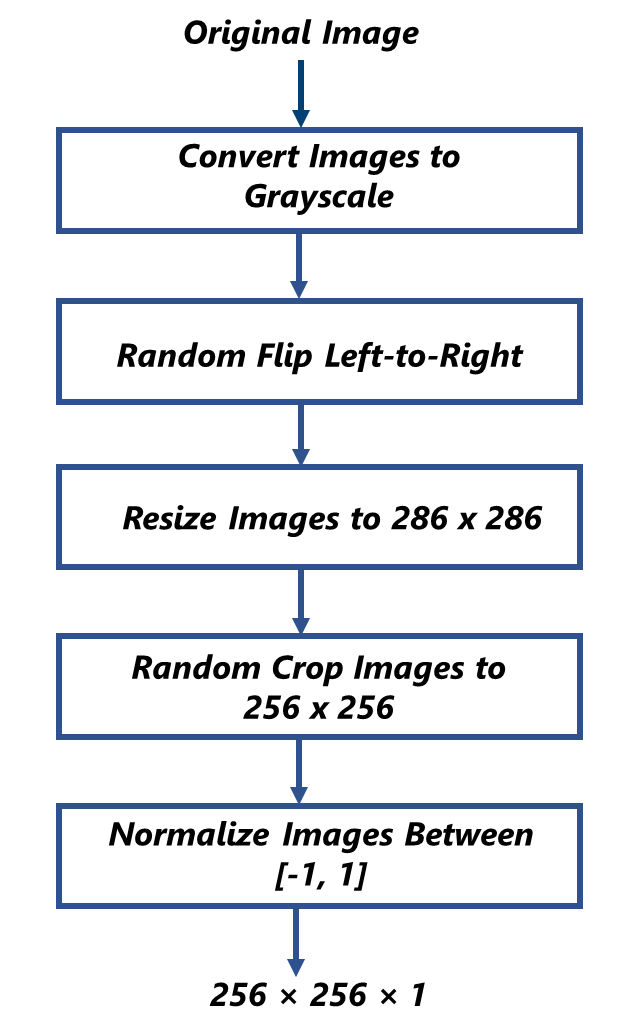
\includegraphics[scale=0.35]{images/Preprocessing.png}
	    \caption[Steps involved in preprocessing of training images of \ac{CycleGAN}.]{Steps involved in preprocessing of training images of \ac{CycleGAN}.}
	    \label{fig:Preprocessing}
	    \end{center}
\end{figure}

The \ac{CycleGAN} trained with a learning rate of $0.0002$. The weights of all the neural networks(generators and discriminators) in the \ac{CycleGAN} model are initialized by a Gaussian distribution with mean ($\mu$) 0 and standard deviation ($\sigma$) 0.02. 
For all experiments in equation \ref{FullObjective}, $\lambda_{cyc}$ is set to $10$ and $\lambda_{identity}$ is set to $0.5$ which mean importance of cycle-consistency loss is important in the final objective function. The weights of the neural networks of \ac{CycleGAN} model are optimized by ADAM solver, which is a method for stochastic optimization\cite{kingma2017adam}. Also while constructing generators and discriminators we have used instance normalization layers \cite{ulyanov2017instance}, the initializer for the gamma weight is initialized by Gaussian distribution with mean ($\mu$) 0 and standard deviation ($\sigma$) 0.02. The \ac{CycleGAN} is trained for 20 epochs and all the individual models like Forward Generator $G$, Backward Generator $F$, Discriminator $D_Y$, and Discriminator $D_X$. The training checkpoints\footnote{\url{https://www.tensorflow.org/guide/checkpoint} last access: 22.07.2021} are saved at the end of every epoch. The stack of 100,000 synthetic document images (Domain X) and 100,0000 real document images (Domain Y) are used to train the complete \ac{CycleGAN} model. The training images are preprocessed. The preprocessing process is illustrated in figure \ref{fig: Preprocessing}. Initially, images are converted into grayscale. Next, random mirroring is applied, in which the image is randomly flipped horizontally from left to right. Next random mirroring is applied, in which the image is resized to $286 \times 286$ and then randomly cropped to $256 \times 256$. Random jittering and mirroring are image augmentation techniques that avoid overfitting \cite{zhu2020unpaired}. Lastly, the images are normalized in the range of $[-1, 1]$. All the classifiers are trained for 10 epochs.



\subsection{Classifier}

As described earlier, in this thesis three separate classifiers are trained, first on synthetic document images, second on faxified document images, and third on \ac{CycleGAN} generated document images. The synthetic and faxified document images are preprocessed. The preprocessing process of these images is illustrated in figure \ref{fig:PreprocessingClassfier}. Initially, images are converted into grayscale. Next, resized to $256 \times 256$ and later normalized between $[-1, 1]$. The \ac{CycleGAN} generated document images are need not be preprocessed, as the images generated by the generator $G$ ($G : X \rightarrow Y$) are of $256 \times 256$ dimension and already normalized between $[-1, 1]$. Because at the final layer of the generator, tanh activation function is used, this can be seen in the architecture of the generator in table \ref{table:GeneratorArchitecture}.

\begin{figure}[H]
        \begin{center}
	    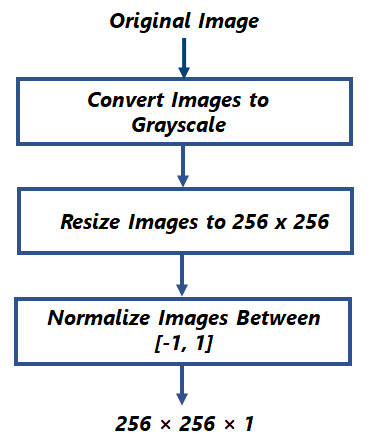
\includegraphics[scale=0.55]{images/ClassifierPreprocessing.png}
	    \caption[Steps involved in preprocessing of training images of Classifiers.]{Steps involved in preprocessing of training images of Classifiers.}
	    \label{fig:PreprocessingClassfier}
	    \end{center}
\end{figure}

















































































%%%%%%%%%%%%%%%%%%%%%%%%%%%%%%%%%%%%%%%%%%%%%%%%%%%%%%%%%%%%%%%%%%%%%%%%%%%%%%%%%%%%%%%%%%%%%%%%%%%%%%%

%In the faxification process, several image transformations are applied to the images randomly means the output images produced during this process are random. Transformations like rotation, brightness difference, dithering \cite{8580565} are visible in the above image after the faxification process. The dithering is the process of applying noise intentionally in the images.


\begin{comment}
\begin{figure}[H]
        \begin{center}
    	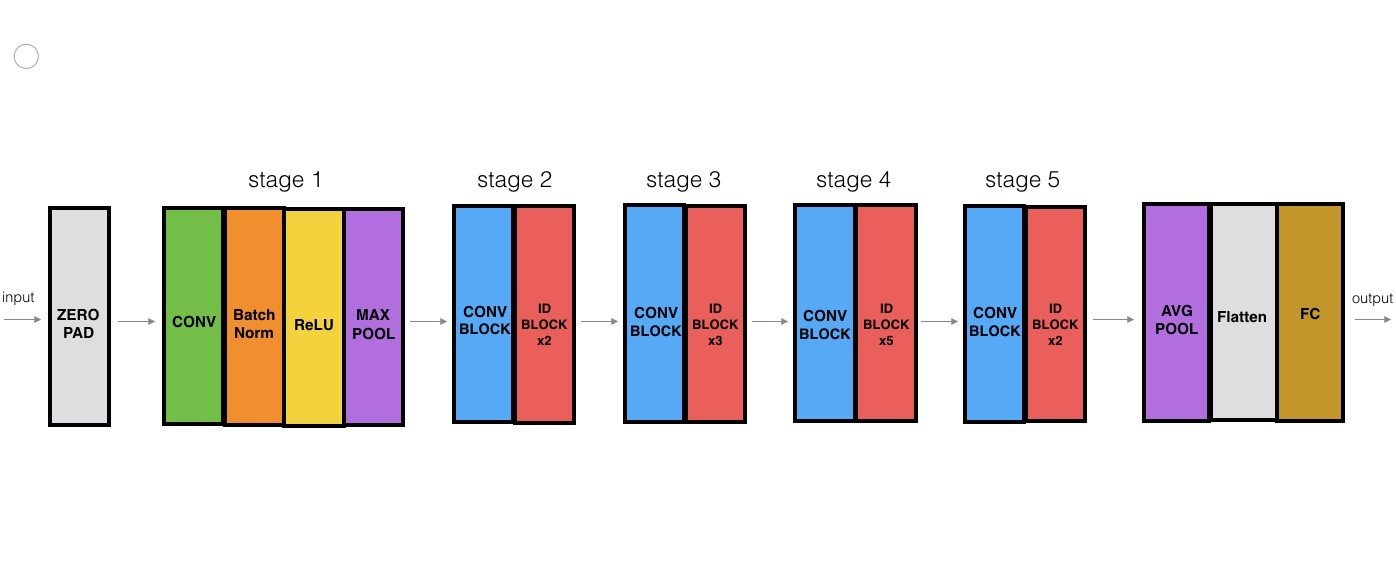
\includegraphics[scale=0.43]{images/ResNet50_1.jpg}
	    \caption[ResNet-50 Classifier Architecture.]{ResNet-50 Classifier Architecture.\footnotemark}
	    \label{fig:ResNet50}
	    \end{center}
\end{figure}
\footnotetext{\url{https://github.com/priya-dwivedi/Deep-Learning/blob/master/resnet_keras/Residual_Networks_yourself.ipynb} last access: 04.05.2021}

\begin{figure}[H]
        \begin{center}
	    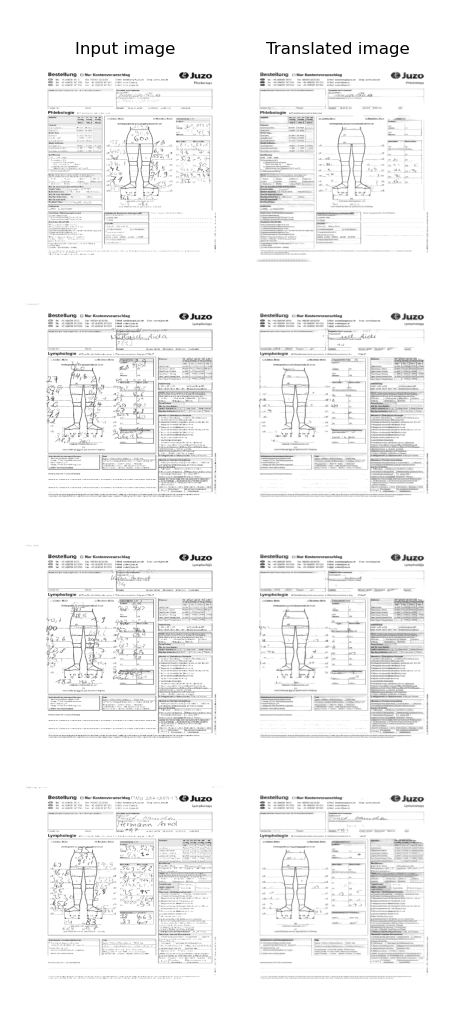
\includegraphics[scale=0.60]{images/CycleGAN_Generated_Images_3_5.png}
	    \caption{\ac{CycleGAN} transalated images.}
	    \label{fig:GeneratedImages}
	    \end{center}
\end{figure}


\end{comment}

\begin{comment}
\begin{figure}[H]
      \centering
      \hspace*{-0.75cm}
      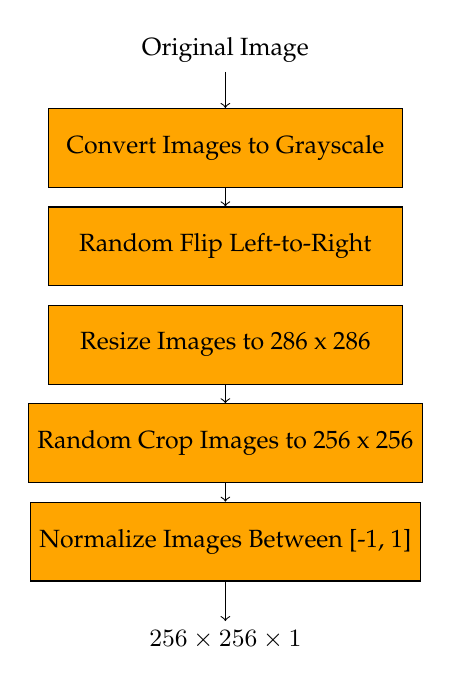
\begin{tikzpicture}
        \node[rotate=0,minimum width=4.5cm] (input) at (0,11.25) {\small{Original Image}};
        \node[conv,rotate=0,minimum width=4.5cm] (Grayscale) at (0,10) {\small{Convert Images to Grayscale}};
        \node[conv,rotate=0,minimum width=4.5cm] (Randomflip) at (0,8.75) {\small{Random Flip Left-to-Right}};
        \node[pool,rotate=0,minimum width=4.5cm] (Resize) at (0,7.5) {\small{Resize Images to 286 x 286}};
        \node[dp,rotate=0,minimum width=4.5cm] (Randomcrop) at (0,6.25) {\small{Random Crop Images to 256 x 256}};
        \node[flatten,rotate=0,minimum width=4.5cm] (normalize) at (0,5.0) {\small{Normalize Images Between [-1, 1]}};
        \node[rotate=0,minimum width=4.5cm] (output) at (0,3.75) {\small$256 \times 256 \times 1$};

        \draw[->] (input) -- (Grayscale);
        \draw[->] (Grayscale) -- (Randomflip);
        \draw[->] (Resize) -- (Randomcrop);
        \draw[->] (Randomcrop) -- (normalize);
        \draw[->] (normalize) -- (output);
        
      \end{tikzpicture}
      \vskip 6px
      \caption{Pre-processing Process of Images.}
      \label{fig:Pre-processingSteps}
\end{figure}

\end{comment}
%While conducting the experiments, ResNet-50 \cite{he2015deep} architecture also has been considered. The architecture of ResNet-50 classifier can be viewed in figure \ref{fig:ResNet50}.


%The proposed image-to-image translation application is implemented using \ac{CycleGAN}. The quality of images generated by the \ac{CycleGAN} is assessed by a classifier that is trained on the same generated images and tested on real images. The classification performance of the classifier on real images is the metric to evaluate the quality of generated images. The evaluation of images generated by \ac{CycleGAN} is described thoroughly in section \ref{evaluation}. In this thesis, numerous experiments were performed to understand the domain gap\footnotemark 
%\footnotetext{\url{https://machinelearning.apple.com/research/bridging-the-domain-gap-for-neural-models} last access: 27.05.2021} between real document images and different data distributions like synthetic document images, faxified document images, and \ac{CycleGAN} generated document images. 

%The proposed image-to-image translation application is implemented using \ac{CycleGAN}. The quality of images generated by the \ac{CycleGAN} is assessed by a classifier that is trained on the same generated images and tested on real images. The classification performance of the classifier on real images is the metric to evaluate the quality of generated images. The evaluation of images generated by \ac{CycleGAN} is described thoroughly in section \ref{evaluation}. In this thesis, numerous experiments were performed to understand the domain gap\footnotemark 
%\footnotetext{\url{https://machinelearning.apple.com/research/bridging-the-domain-gap-for-neural-models} last access: 27.05.2021} between real document images and different data distributions like synthetic document images, faxified document images, and \ac{CycleGAN} generated document images. The experiments are visualized using Tensorboard\footnotemark. TensorBoard is tool which provides the visualization needed for machine learning experimentation. The \ac{CycleGAN} and Classifier are implemented in Python and using the TensorFlow library\cite{tensorflow2015-whitepaper}. The code for the \ac{CycleGAN} is available \href{https://keras.io/examples/generative/cyclegan/}{here}. All of the neural networks are trained upon GPUs (Graphics Processing Units) like Nvidia Tesla T4 and Tesla V100-SXM2.

%\footnotetext{\url{https://www.tensorflow.org/tensorboard} last access: 04.05.2021}


\begin{comment}

The architecture of \ac{CycleGAN} is adapted from Johnson et al. ~\cite{johnson2016perceptual}. The generator network is implemented using a sequence of downsampling convolutional blocks to encode the $256 \times 256 \times 1$ grayscale input image, 9 \ac{ResNet} convolutional blocks to transform the image, and a number of upsampling convolutional blocks to generate the output image of the same dimension as the input image. The reason behind using residual blocks is it resolves the vanishing gradient problem in deep neural networks. The discriminator networks uses PatchGAN ~\cite{isola2018imagetoimage}. In PatchGAN, after feeding one input image to the network, it gives you the probabilities of two things: either real or fake, but not in scalar output indeed, it used the $N \times N$ output vector. Here $N \times N$ can be different depending on the dimension of an input image. The naming convention used in the Johnson et al.'s \cite{johnson2016perceptual} Github \href{https://github.com/jcjohnson/fast-neural-style}{repository}. The architecture of discriminator and generator can be preciously visualised in figures \ref{fig:discriminator} and \ref{fig:generator}. 

Let {\fontfamily{qcr}\selectfont c7s1-k} denote a $7 \times 7$ Convolution-InstanceNorm-ReLU layer with k filters and stride 1. {\fontfamily{qcr}\selectfont dk} denotes a $3 \times 3$ Convolution-InstanceNorm-ReLU layer with $k$ filters and stride 2. Reflection padding was used to reduce artifacts. {\fontfamily{qcr}\selectfont Rk} denotes a residual block that contains two $3 \times 3$ convolutional layers with the same number of filters on both layer. {\fontfamily{qcr}\selectfont uk} denotes a $3  \times 3$ fractional-strided-Convolution-InstanceNorm-ReLU layer with $k$ filters and stride $\frac{1}{2}$. The generator network with 9 residual blocks consists of: {\fontfamily{qcr}\selectfont c7s1-64, d128, d256, R256, R256, R256, R256, R256, R256, R256, R256, R256, u128, u64, c7s1-1}. followed by a Tanh function (figure \ref{fig:ActivationFunctions}). The discriminator uses $70 \times 70$ PatchGAN \cite{isola2018imagetoimage}, which is also called as Markovian discriminator \cite{isola2018imagetoimage}. Let {\fontfamily{qcr}\selectfont Ck} denote a $4 \times 4$ Convolution-InstanceNorm-LeakyReLU layer with $k$ filters and stride 2. After the last layer, a convolution is applied to produce a 1-dimensional output. We do not use InstanceNorm for the first C64 layer. We use leaky ReLUs with a slope of 0.2. The discriminator architecture is: {\fontfamily{qcr}\selectfont C64-C128-C256-C512}.


\end{comment}


\begin{comment}

\begin{center}
\begin{table}[H]
    \begin{center}
    \begin{tabular}{p{0.25\linewidth} p{0.25\linewidth} p{0.25\linewidth} p{0.25\linewidth}} 
        \toprule
        Operation Layer & Number of Filters & Size of Each Filter & Stride Value\\
        \midrule
        Input Image ($256 \times 256$) & - & - \\
        \midrule
        Convolution Layer & 32 & $3 \times 3$ & $1 \times 1$\\
        \bottomrule
    \end{tabular}
    \caption[]{}
    \label{table:ClassifierArchitecture}
    \end{center}
\end{table}
\end{center}



\begin{center}
\begin{table}[H]
    \begin{center}
    \begin{tabular}{p{0.15\linewidth} p{0.10\linewidth} p{0.10\linewidth} p{0.10\linewidth} p{0.10\linewidth}} 
        \toprule
         Operation Layer & Number of Filters & Size of Each Filter & F1-score & Support\\[0.0ex] 
        \midrule
      
        \bottomrule
    \end{tabular}
    \caption[]{}
    \label{table:discriminatorArchitecture}
    \end{center}
\end{table}
\end{center}



\begin{figure}[H]
      \centering
      \hspace*{-0.75cm}
      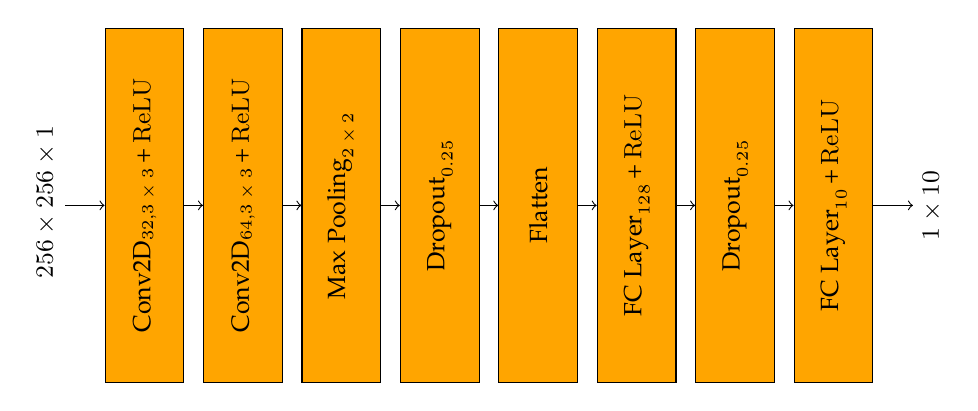
\begin{tikzpicture}
        \node[rotate=90,minimum width=4.5cm] (input) at (0,0) {\small$\ 256 \times 256 \times 1$};
        \node[conv,rotate=90,minimum width=4.5cm] (conv1) at (1.25,0) {\small$\text{Conv2D}_{32, \text{$3 \times 3$}}$\,+\,$\ReLU$};
        \node[conv,rotate=90,minimum width=4.5cm] (conv2) at (2.5,0) {\small$\text{Conv2D}_{64, \text{$3 \times 3$}}$\,+\,$\ReLU$};
        \node[pool,rotate=90,minimum width=4.5cm] (pool1) at (3.75,0) {\small$\text{Max Pooling}_{\text{$2 \times 2$}}$};
        \node[dp,rotate=90,minimum width=4.5cm] (dp) at (5.0,0) {\small$\text{Dropout}_{\text{$0.25$}}$};
        \node[flatten,rotate=90,minimum width=4.5cm] (flatten) at (6.25,0) {\small$\text{Flatten}$};
        \node[fc,rotate=90,minimum width=4.5cm] (fc) at (7.5,0) {\small$\text{FC Layer}_{128}$\,+\,$\ReLU$};
        \node[dp,rotate=90,minimum width=4.5cm] (dp1) at (8.75,0) {\small$\text{Dropout}_{\text{$0.25$}}$};
        \node[fc,rotate=90,minimum width=4.5cm] (fc1) at (10,0) {\small$\text{FC Layer}_{10}$\,+\,$\ReLU$};
        \node[rotate=90,minimum width=4.5cm] (output) at (11.25,0) {\small$1 \times 10$};

        
        \draw[->] (input) -- (conv1);
        \draw[->] (conv1) -- (conv2);
        \draw[->] (conv2) -- (pool1);
        \draw[->] (pool1) -- (dp);
        \draw[->] (dp) -- (flatten);
        \draw[->] (flatten) -- (fc);
        \draw[->] (fc) -- (dp1);
        \draw[->] (dp1) -- (fc1);
        \draw[->] (fc1) -- (output);
        
  
        
      \end{tikzpicture}
      \vskip 6px
      \caption[Classifier Architecture.]{Classifier Architecture.}
      \label{fig:ClassifierArchitecture}
\end{figure}


\begin{figure}[H]
      \centering
      \hspace*{-0.75cm}
      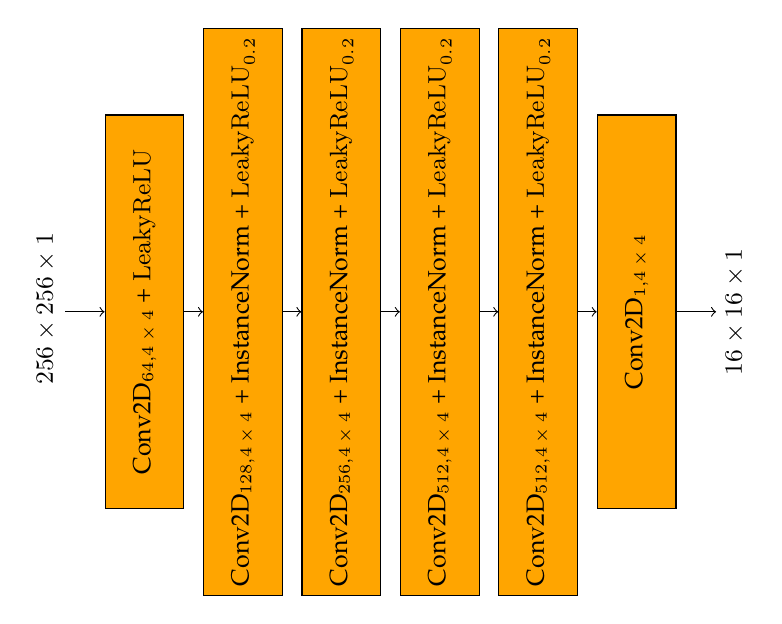
\begin{tikzpicture}
        \node[rotate=90,minimum width=5cm] (input) at (0,0) {\small$\ 256 \times 256 \times 1$};
        \node[conv,rotate=90,minimum width=5cm] (conv1) at (1.25,0) {\small$\text{Conv2D}_{64, \text{$4 \times 4$}}$ + $\LeakyReLU$};
        \node[conv,rotate=90,minimum width=5cm] (conv2) at (2.5,0)   {\small$\text{Conv2D}_{128, \text{$4 \times 4$}}$ + InstanceNorm + ${\LeakyReLU}_{0.2}$};
	 \node[conv,rotate=90,minimum width=5cm] (conv3) at (3.75,0)  {\small$\text{Conv2D}_{256, \text{$4 \times 4$}}$ + InstanceNorm + ${\LeakyReLU}_{0.2}$};
	 \node[conv,rotate=90,minimum width=5cm] (conv4) at (5.0,0)  {\small$\text{Conv2D}_{512, \text{$4 \times 4$}}$   + InstanceNorm + ${\LeakyReLU}_{0.2}$};
	 \node[conv,rotate=90,minimum width=5cm] (conv5) at (6.25,0)  {\small$\text{Conv2D}_{512, \text{$4 \times 4$}}$   + InstanceNorm + ${\LeakyReLU}_{0.2}$};
	 \node[conv,rotate=90,minimum width=5cm] (conv6) at (7.5,0)  {\small$\text{Conv2D}_{1, \text{$4 \times 4$}}$};
	 \node[rotate=90,minimum width=5cm] (output) at (8.75,0) {\small$16 \times 16 \times 1$};

        
        \draw[->] (input) -- (conv1);
        \draw[->] (conv1) -- (conv2);
        \draw[->] (conv2) -- (conv3);
        \draw[->] (conv3) -- (conv4);
        \draw[->] (conv4) -- (conv5);
        \draw[->] (conv5) -- (conv6);
        \draw[->] (conv6) -- (output);

        
  
        
      \end{tikzpicture}
      \vskip 6px
      \caption[Discriminator Architecture.]{Discriminator Architecture.}
      \label{fig:DiscriminatorArchitecture}
\end{figure}

\end{comment}

\newpage

\chapter{Experiments and Evaluation}
    \label{evaluation}
    %\noindent
%\justifying
\setlength{\parskip}{1em}

This chapter discusses the experiments conducted in this thesis, evaluation metrics and results. The evaluation metrics like accuracy, precision, recall, confusion matrix and F1-score are discussed in section \ref{EvaluationMetrics}. These metrics are used to evaluate the domain gap between the distributions and quality of \ac{CycleGAN} generated document images. In section \ref{experiments} conducted experiments are explained along with training plots, confusion matrices and classification reports. Finally, in section \ref{results}, quantitative and qualitative results are discussed thoroughly along with the typical failure cases.

\section{Evaluation Metrics}\label{EvaluationMetrics}

%\subsection{Accuracy}
%\subsection{Precision and Recall}
%\subsection{F1-score}

In machine learning, there are numerous performance metrics to evaluate neural networks. Each evaluates different aspects of neural network performance. Hence, It is needed to have a specific set of performance metrics for a particular problem solved using neural networks. It's vital to evaluate the neural network's performance after training using testing data to determine its actual performance and generalization error on unseen data \cite{powers2020evaluation}. In this thesis, the performance of classifiers trained upon different data distributions determined using annotated real document images (testing dataset) and evaluation metrics like accuracy, precision, recall, confusion matrix and F1-score are used. The testing dataset used to evaluate the classifiers is unbalanced, hence metrics like weighted average and macro average F1-scores are essential for the performance comparison of the classifiers trained on different data distributions. Accuracy is the most common and widely used metric to evaluate classifiers\footnotemark. It is the ratio of number of correct predictions to the total number of predictions (equation \ref{accuracy}). However, accuracy is not suitable metric for performance evaluation when testing dataset is unbalanced. Hence, along with accuracy and F1-score, precision and recall are also considered during the performance evaluation. The precision is the ratio of the number of true positives divided by the sum of the true positive and false positives (equations \ref{precision}). The recall is the ratio of the number of true positives divided by the sum of true positives and false negatives (equations \ref{recall}). In below equations \ref{accuracy}, \ref{precision} and \ref{recall} the $TP$ means true positives, $TN$ means true negatives, $FP$ means false positives and $FN$ means false negatives.

%\cite{vakili2020performance}
%\footnotemark[\value{footnote}]
%\footnotemark
%\footnotetext[1]{\url{https://en.wikipedia.org/wiki/Precision_and_recall} last access: \dcdate}
%\footnotetext[2]{\url{https://machinelearningmastery.com/precision-recall-and-f-measure-for-imbalanced-classification/} last access: \dcdate}
\footnotetext{\url{https://machinelearningmastery.com/precision-recall-and-f-measure-for-imbalanced-classification/} last access: \dcdate}

\begin{equation}\label{accuracy}
\textit{Accuracy} = \frac{TP + TN}{TP +TN+ FP + FN}
\end{equation}

\begin{equation}\label{precision}
\textit{Precision} = \frac{TP}{TP + FP}
\end{equation}

\begin{equation}\label{recall}
\textit{Recall} = \frac{TP}{TP + FN}
\end{equation}

\newpage
The F1-score is the harmonic mean of the precision and recall (equation \ref{F1-score}). The weighted average F1-score is determined by first calculating the F1-score of each class separately and each multiplied by the weight (the number of true instances for each class) and finally added together, hence favoring the majority class\footnotemark. The equation \ref{Weightedf1-score} represents the weighted average F1-score. The macro average F1-score computes the unweighted mean of separate F1-score of each class. The macro average F1-score does not take label inbalance into account\footnotemark[\value{footnote}]. This leads to bigger penalization when the classifier does not perform well on minority classes. The equation \ref{macrof1-score} represents the macro average F1-score. In equations \ref{Weightedf1-score} and \ref{macrof1-score}, $N$ represents number of classes. More information about accuracy, precision, recall and F1-score can be found \href{https://en.wikipedia.org/wiki/Precision_and_recall}{here.}

\footnotetext{\url{https://scikit-learn.org/stable/modules/generated/sklearn.metrics.f1_score.html} last access: \dcdate}


\begin{equation}\label{F1-score}
\textit{F1-score} = \frac{2 \times precision \times recall}{precision + recall}
\end{equation}


\begin{equation}\label{macrof1-score} 
\textit{Macro average F1-score} =  \frac{F1_{class1} + F1_{class2}+ ... + F1_{classN}}{N}
\end{equation}


\begin{equation}\label{Weightedf1-score} 
\textit{Weighted average F1-score} =  \frac{F1_{class1} \times W_1 + F1_{class2} \times W_2 + ... + F1_{classN} \times W_N}{N}
\end{equation}

The confusion matrix is the most intuitive metric to determine the accuracy of the classifiers. It is a table that describes how well a classifier performs on a test dataset that is labeled or annotated. It is useful when the classifier has to classify more than two classes. The instances of the true class are represented at each row of the confusion matrix whereas the instances of predicted class probabilities are represented by each column or vice versa. In this thesis, the confusion matrix is extensively used to determine the performance of the classifiers trained on different data distributions to analyze domain gap and quality of \ac{CycleGAN} generated document images. More information about the confusion matrix can be found \href{https://en.wikipedia.org/wiki/Confusion_matrix}{here}.

%\footnotemark \footnotetext{\url{https://en.wikipedia.org/wiki/Confusion_matrix} last access: \dcdate}


\section{Experiments}\label{experiments}

In this thesis, three data distributions are considered for the experiments. The synthetic data distribution, faxified data distribution and \ac{CycleGAN} generated data distribution. Experiments are performed to analyze the domain gap between these data distributions and real data distribution. The experiment is conducted to analyze the domain gap between \ac{CycleGAN} generated data distribution and real data distribution, determines the quality of \ac{CycleGAN} generated document images, revealing how much they are close to the real document images. Now let's describe the conducted experiments briefly, a) Train a classifier on synthetic document images and its performance is evaluated on testing dataset (Annotated real document images, table \ref{table:testdataset}). b) Another classifier with the same architecture is trained on faxified document images and its performance is evaluated on the testing dataset. c) The \ac{CycleGAN} is trained for 20 epochs, using synthetic document images (Source domain $X$) and real document images (Target domain $Y$) and the checkpoint is saved at the end of every epoch. Once \ac{CycleGAN} training is finished, the saved model is loaded to generate images or transform synthetic document images into realistic document images. From the saved \ac{CycleGAN} model, generator $G$, retrieved, as it transforms synthetic document images into realistic document images (Source domain $X$ to Target domain $Y$, $G: X \rightarrow Y$). 100,000 synthetic document images transformed into realistic document images, generating a dataset of 100,000 \ac{CycleGAN} generated document images, with 10 classes and each class has 10000 images. d) Next, another classifier, with same architecture is trained on the \ac{CycleGAN} generated document images and its performance is evaluated on testing dataset. This experiment determines the quality of the images generated by \ac{CycleGAN}. Also, it indicates how well \ac{CycleGAN} was able to close the domain gap between synthetic data distribution and real data distribution. To put it another way, how well the \ac{CycleGAN} generated data distribution matched the real data distribution. As a whole, how similar \ac{CycleGAN} generated document images are to the real document images. In this thesis, the evaluation metrics like accuracy, weighted average F1-score and macro average F1-score \cite{lipton2014thresholding} are used to determine the performance of classifiers on testing dataset. The architecture of the classifier is illustrated in table \ref{table:ClassifierArchitecture}.


\subsection{Experiment Steps}
\begin{enumerate}
    \itemsep0em 
    \item Train a classifier using synthetic document images and evaluate its performance over testing dataset.
    \item Train a classifier using faxified document images and evaluate its performance over testing dataset.
    \item Train \ac{CycleGAN} using synthetic document images and real document images.
    \item Generate realistic document images using generator $G$ retrieved from the trained and saved \ac{CycleGAN} model.
    \item Train a classifier using \ac{CycleGAN} generated document images and evaluate its performance over testing dataset. This experiment reveals how well the \ac{CycleGAN} generated document images are generalizing to the real document images, eventually determining the quality of images generated by \ac{CycleGAN}.
    \item Compare the classification performance of the above three classifiers (trained on 3 different data distributions) on testing dataset and determine which distribution is closer to the real data distribution.
\end{enumerate}

%The domain gap between real data distribution and other three distributions like synthetic data distribution, faxified data distribution and \ac{CycleGAN} generated data distribution.The performance evaluation of a classifier trained upon \ac{CycleGAN} generated data distribution using annotated real document images describes, how close is the \ac{CycleGAN} generated data distribution to the real data distribution. Simply this approach determines the quality of the \ac{CycleGAN} generated document images compared to real document images.


\subsection{Training a Classifier on Synthetic Document Images}\label{trainingsyntheticclassifier}

The dataset of synthetic document images is created using templates (figure of sample \ref{fig:template}) and handwritten crops (figure of sample \ref{fig:keinwifi}) using the process mentioned in figure \ref{fig:InsertHandwrittenCrops}. This dataset consists of 100,000 document images, 10 classes and each class has 10000 images. In this experiment, a classifier is trained on synthetic document images dataset. The performance of this classifier is evaluated on testing dataset (Annotated real document images) to understand the domain gap between real data distribution and synthetic data distribution. The classification report in table \ref{table:SyntheticClassificationReport} states that the accuracy of this classifier on real document images is 25\%, macro average F1-score is 27\% and weighted average F1-score is 31\%. The obtained results conclude that there is a huge gap between real data distribution and synthetic data distribution. The confusion matrix is illustrated in figure \ref{fig:CMSyntheticDocumentImagesClassifier}. In which, it is visible that most of the images from the testing dataset were classified wrongly. Only test images from classes DE\_LY\_Arm\_2020-01 (support 44), DE\_LY\_Bein\_2019-01 (support 50) and DE\_LY\_Hand\_2020-01 (support 16) are classified correctly with a recall score of 50\%, 90\% and 44\% respectively. The epochs against accuracy and epochs against loss plots while training classifier on synthetic document images is illustrated in figure \ref{fig:SyntheticClassifierAcc} and \ref{fig:SyntheticClassifierLoss} respectively. The epochs against accuracy and epochs against loss plots while training classifier on synthetic document images is illustrated in figure \ref{fig:SyntheticClassifierAcc} and \ref{fig:SyntheticClassifierLoss} respectively.


\begin{figure}[H]
  \centering
  \begin{minipage}[b]{0.45\textwidth}
    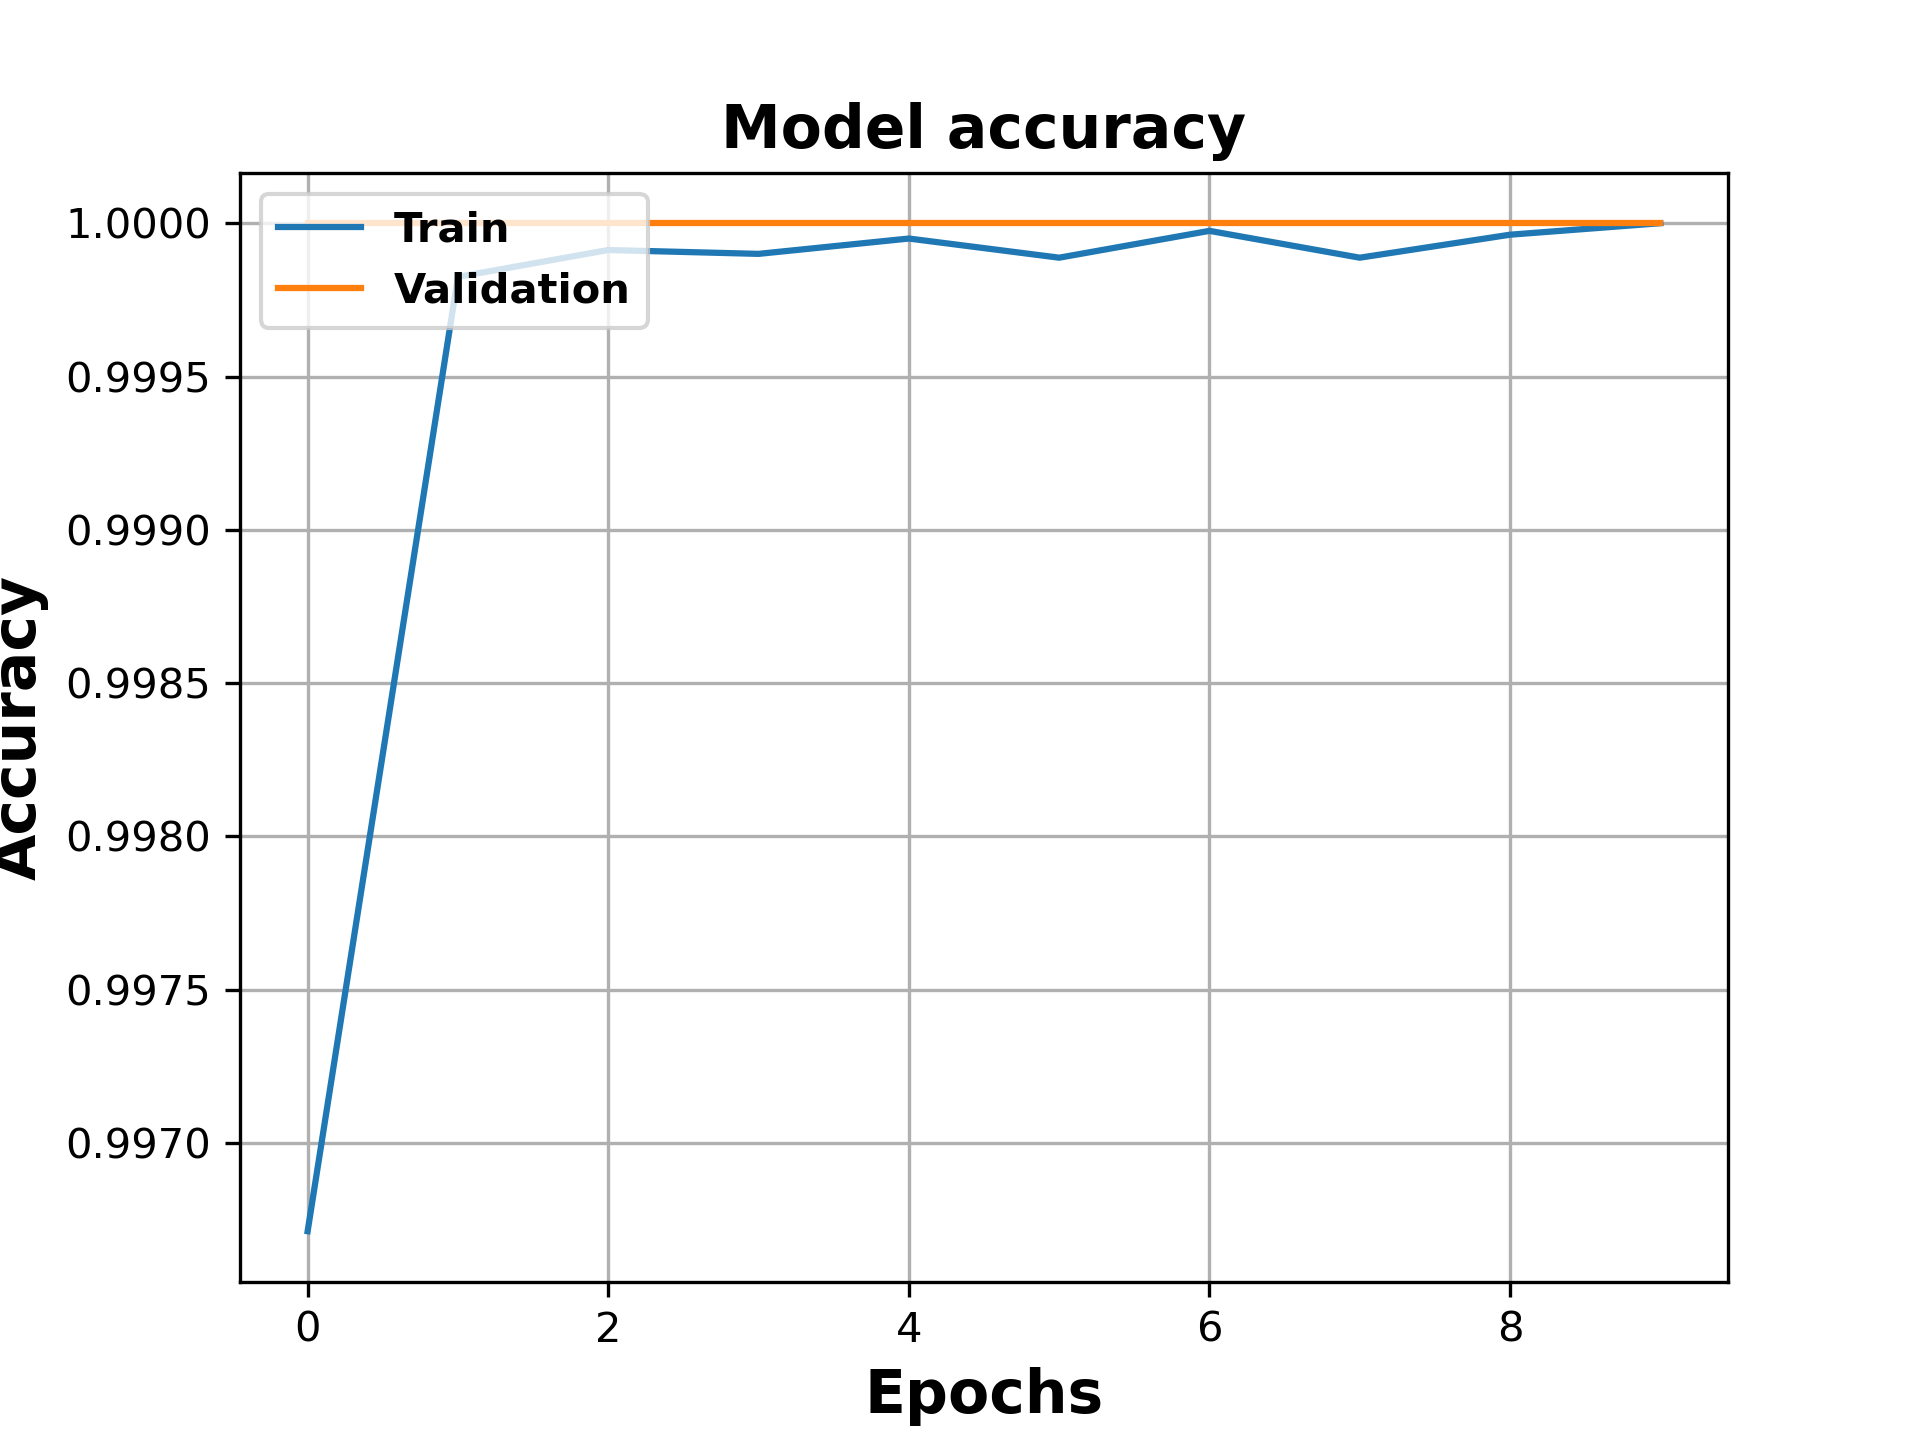
\includegraphics[width=\textwidth]{images/Evaluation/Synthetic_Data_Classifier_2021-05-31_16-40-33_Accuracy.png}
    \caption[Epochs vs. Accuracy plot during training a classifier on synthetic document images.]{Epochs vs. Accuracy plot during training a classifier on synthetic document images.}
    \label{fig:SyntheticClassifierAcc}
  \end{minipage}
  \hfill
  \begin{minipage}[b]{0.45\textwidth}
    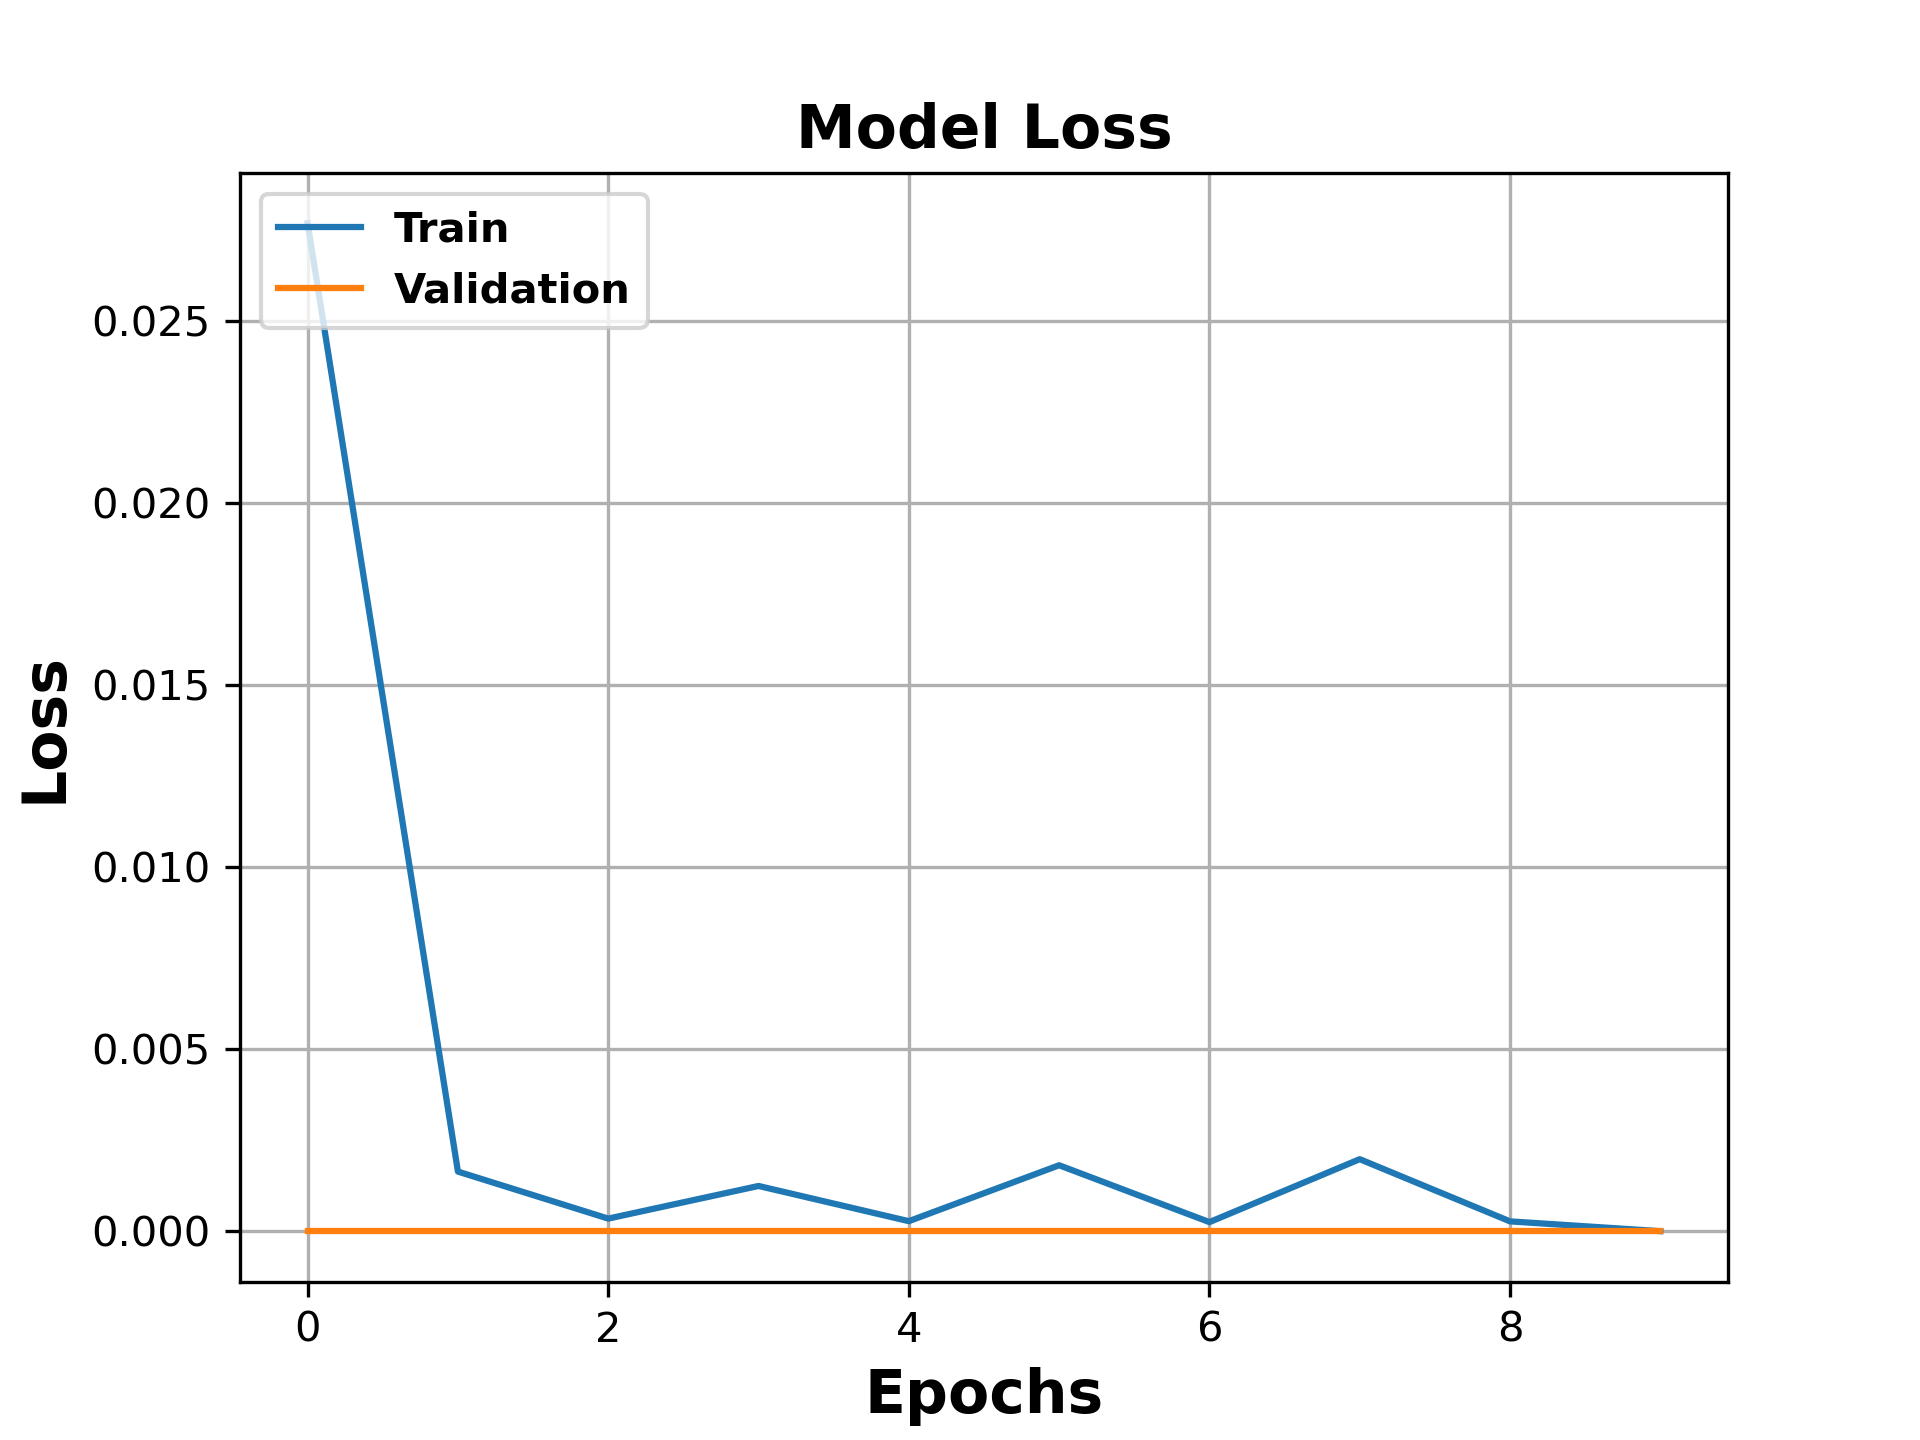
\includegraphics[width=\textwidth]{images/Evaluation/Synthetic_Data_Classifier_2021-05-31_16-40-33_Loss.png}
    \caption[Epochs vs. Loss plot during training a classifier on synthetic document images.]{Epochs vs. Loss plot during training a classifier on synthetic document images.}
    \label{fig:SyntheticClassifierLoss}
  \end{minipage}
\end{figure}

\begin{figure}[H]
    \begin{center}
	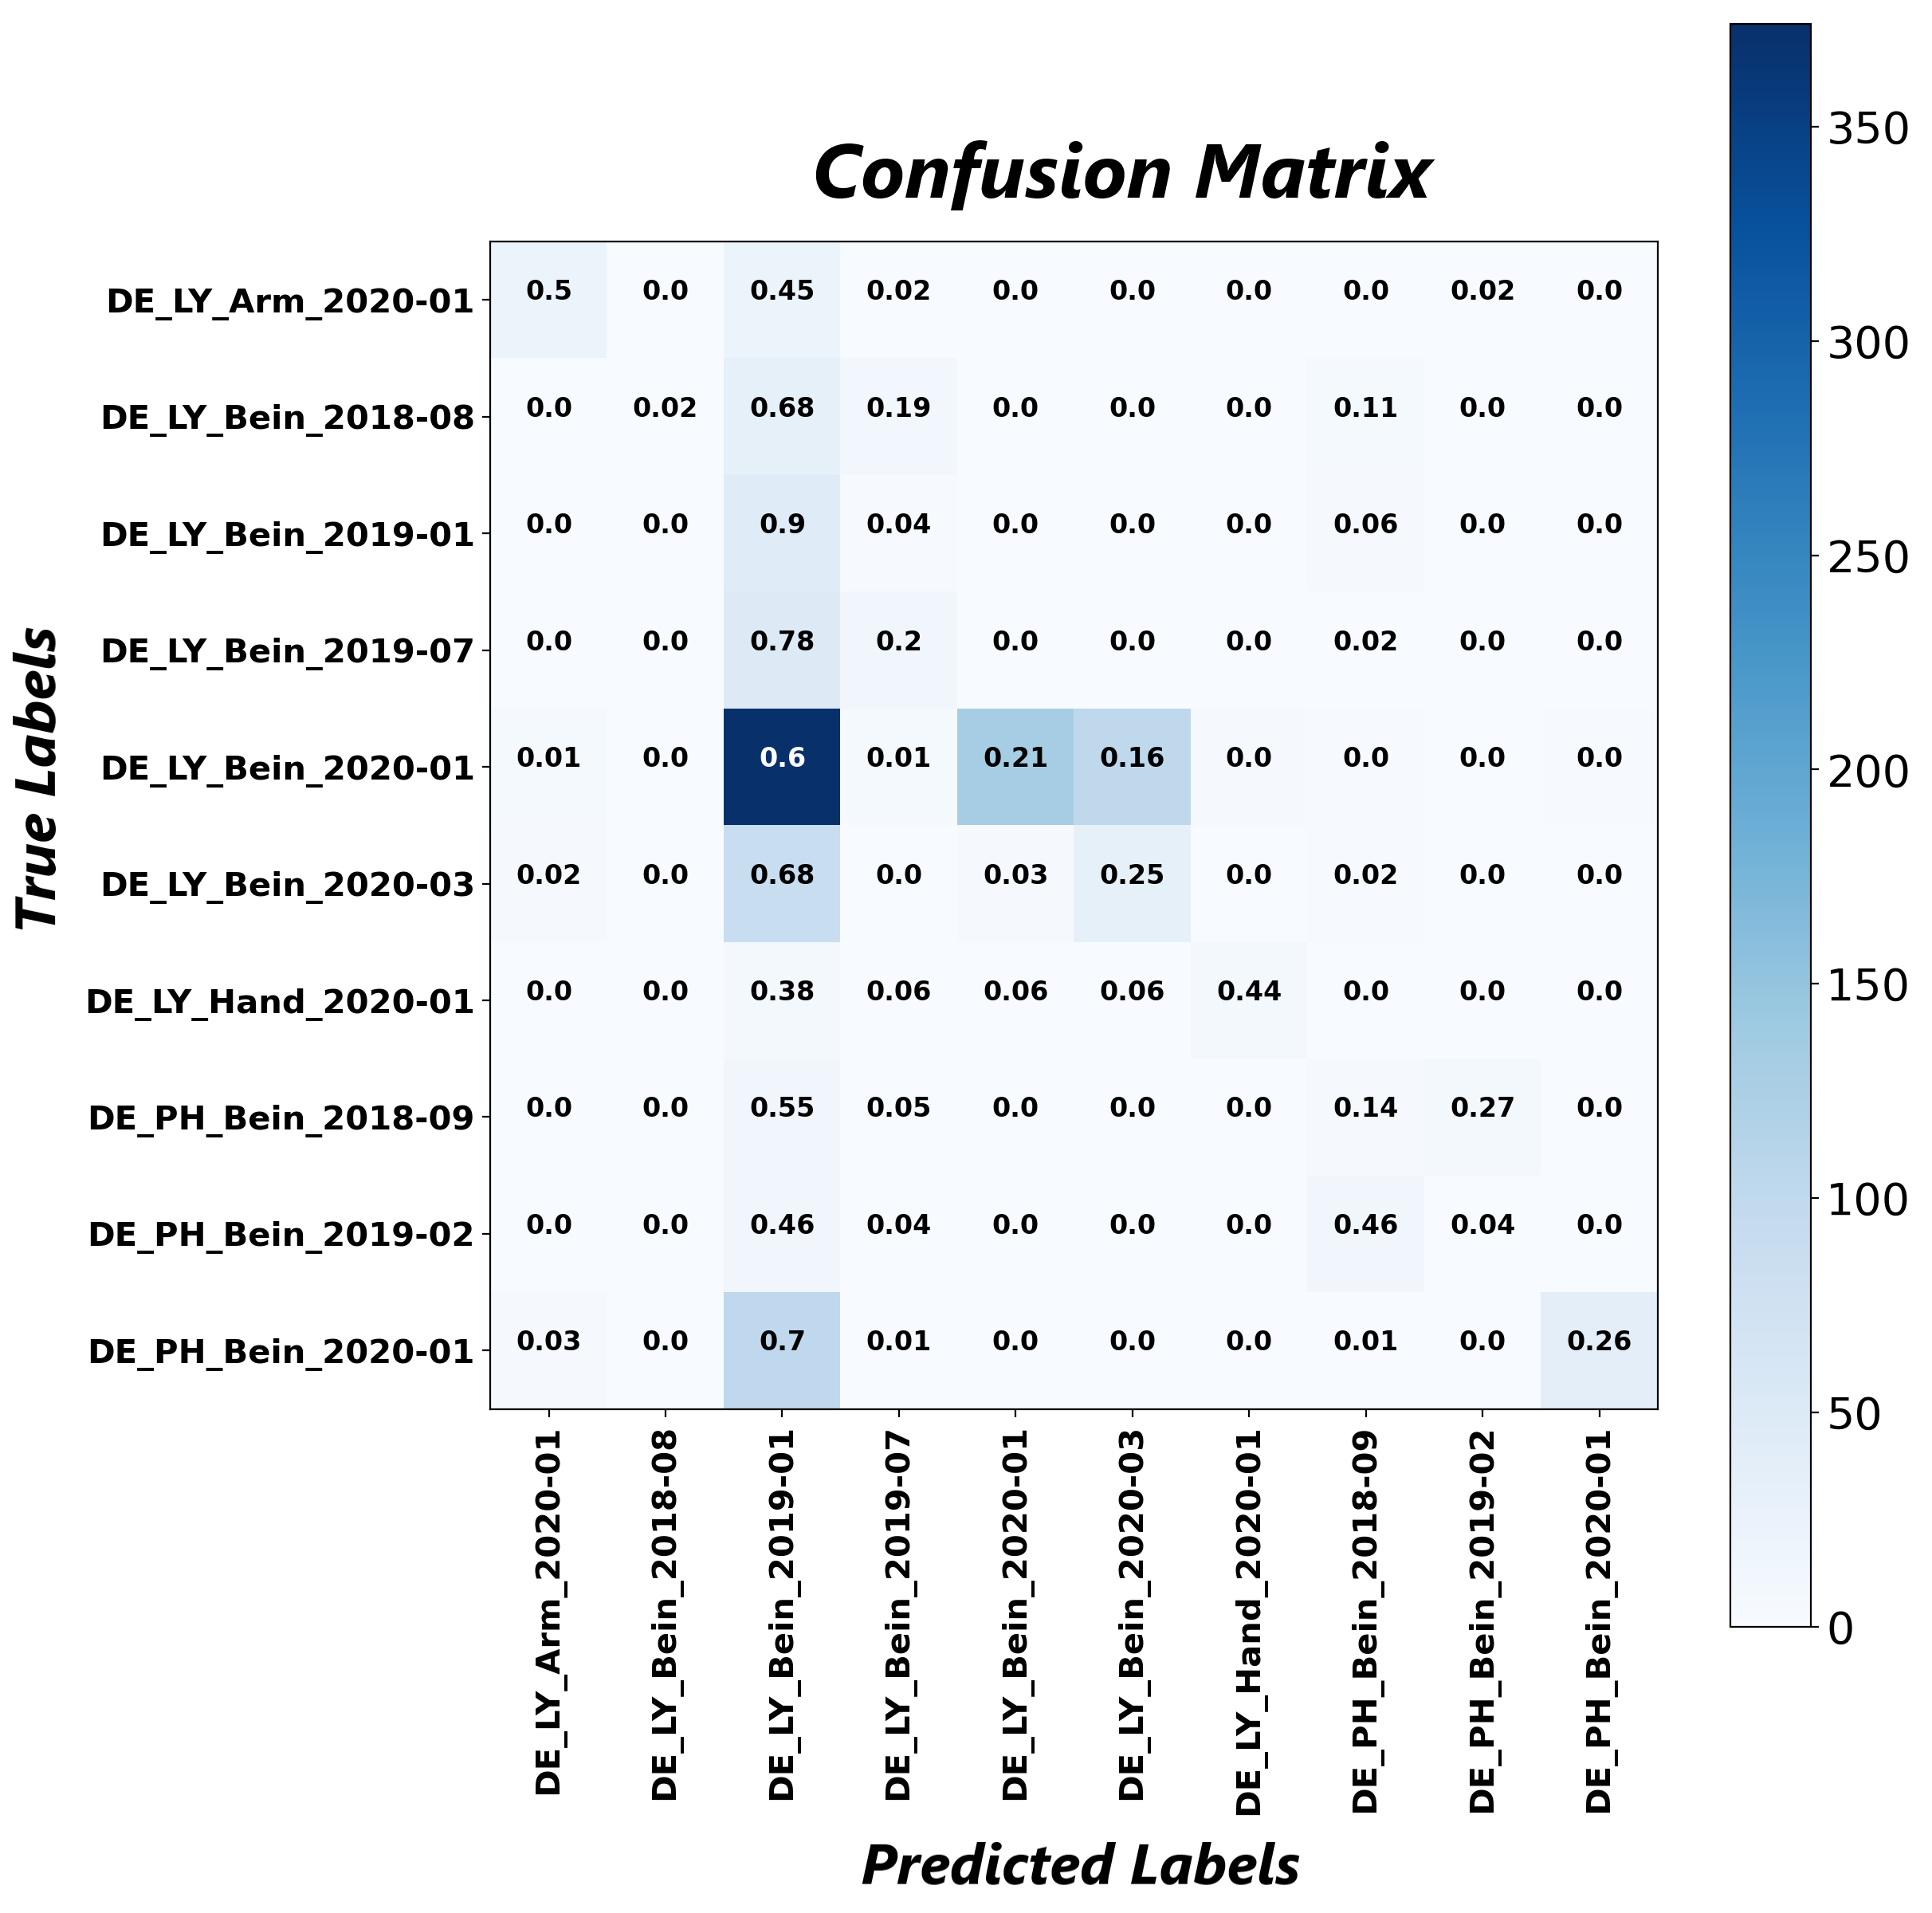
\includegraphics[scale=0.20]{images/Evaluation/Confusion_Matrix_Synthetic_Data_Classifier_2021-05-31_16-40-33.png}
	\caption[Confusion matrix to analyze the performance of the classifier trained on synthetic document images and evaluated using real annotated document images (test dataset).]{Confusion matrix to analyze the performance of the classifier trained on synthetic document images and evaluated using real annotated document images (testing dataset). Green boxes represent classes that are correctly classified and red boxes represent classes that are misclassified.}
	\label{fig:CMSyntheticDocumentImagesClassifier}
	\end{center}
\end{figure}

\begin{center}
\begin{table}[H]
    \centering
    \begin{center}
    \begin{tabular}{P{0.22\linewidth} P{0.10\linewidth} P{0.10\linewidth} P{0.10\linewidth} P{0.10\linewidth}} 
        \toprule
            & Precision & Recall & F1-score & Support\\[0.0ex] 
        \midrule
        DE\_LY\_Arm\_2020-01 & 0.65 & 0.50 & 0.56 & 44\\[0.0ex]
        \midrule
        DE\_LY\_Bein\_2018-08 & 0.50 & 0.02 & 0.04 & 47\\[0.0ex]
        \midrule
        DE\_LY\_Bein\_2019-01 & 0.06 & 0.90 & 0.11 & 50\\[0.0ex]
        \midrule
        DE\_LY\_Bein\_2019-07 & 0.36 & 0.20 & 0.26 & 60\\[0.0ex]
        \midrule
        DE\_LY\_Bein\_2020-01 & 0.96 & 0.21 & 0.34 & 624\\[0.0ex]
        \midrule
        DE\_LY\_Bein\_2020-03 & 0.24 & 0.25 & 0.24 & 128\\[0.0ex]
        \midrule
        DE\_LY\_Hand\_2020-01 & 0.70 & 0.44 & 0.54 & 16\\[0.0ex]
        \midrule
        DE\_PH\_Bein\_2018-09 & 0.10 & 0.14 & 0.12 & 22\\[0.0ex]
        \midrule
        DE\_PH\_Bein\_2019-02 & 0.12 & 0.04 & 0.06 & 28\\[0.0ex]
        \midrule
        DE\_PH\_Bein\_2020-01 & 0.95 & 0.51 & 0.26 & 143\\[0.0ex]
        \midrule
        \midrule
        Accuracy              &      &      & \bf{0.25} & 1162\\[0.0ex]
        Macro average             & 0.46 & 0.29 &  \bf{0.27} & 1162\\[0.0ex]
        Weighted average          & 0.74 & 0.25 &  \bf{0.31} & 1162\\[0.0ex]
        \bottomrule
    \end{tabular}
    \caption[Classification report, evaluating a classifier on the testing dataset after training with synthetic document images.]{Classification report, evaluating a classifier on the testing dataset after training with synthetic document images.}
    \label{table:SyntheticClassificationReport}
    \end{center}
\end{table}
\end{center}



\subsection{Training a Classifier on Faxified Document Images}\label{trainingfaxifiedclassifier}


The faxification process mimics the way the fax machine works. Usually, the fax machines transmit only black-and-white images, but the transfered images might be dirty and not aligned perfectly. This leads to several common artifacts being introduced into transferred images. The faxification process attempts to mimic those introductions of artifacts into images. The faxification process transforms clean gray-scale synthetic document images in such a way like it was sent via fax. However, the faxification process is not deterministic, it involves randomness during the process of faxification of the images. It uses several image transformations like gamma transformation, brightness transformation, 180-degree rotations, resizing, rescaling, binarization, adding noise, adding verticle lines and conversion to a grayscale image. The faxification process can be visualized in figure \ref{fig:FaxificationProcess}. In figure \ref{fig:FaxificationProcessZoomed}, it is visible a snippet from the synthetic document image that has transformed into randomly distinct image transformations when it has sent through the faxification process. The faxification process is implemented in Python using a traditional programming approach.

The dataset of faxified document images is created by transforming synthetic document images using the faxification process (figure \ref{fig:FaxificationProcess}). In this experiment, the classifier is trained using the dataset of faxified document images. The performance of this classifier is evaluated on the testing dataset to understand the domain gap between real data distribution and faxified data distribution. The classification report in table \ref{table:FaxifiedClassificationReport} states that the accuracy of this classifier on testing dataset is 43\%, macro average F1-score is  58\% and weighted average F1-score is 43\%. The results conclude that the faxified data distribution matched the real data distribution better than the synthetic data distribution. The confusion matrix is illustrated in figure \ref{fig:CMFaxifiedDocumentImagesClassifier}. In which, it is visible that document images of class DE\_LY\_Bein\_2019-01 (support 50) are being wrongly classified as DE\_LY\_Bein\_2019-07. Also, the document images of class DE\_LY\_Bein\_2020-01 (support 624) are wrongly classified as DE\_LY\_Bein\_2020-03. The remaining images from the testing dataset are classified convincingly. The epochs against accuracy and epochs against loss plots while training classifier on faxified document images is illustrated in figure \ref{fig:FaxifiedClassifierAcc} and \ref{fig:FaxifiedClassifierLoss} respectively.



\vspace*{1cm}

\begin{figure}[H]
        \begin{center}
	    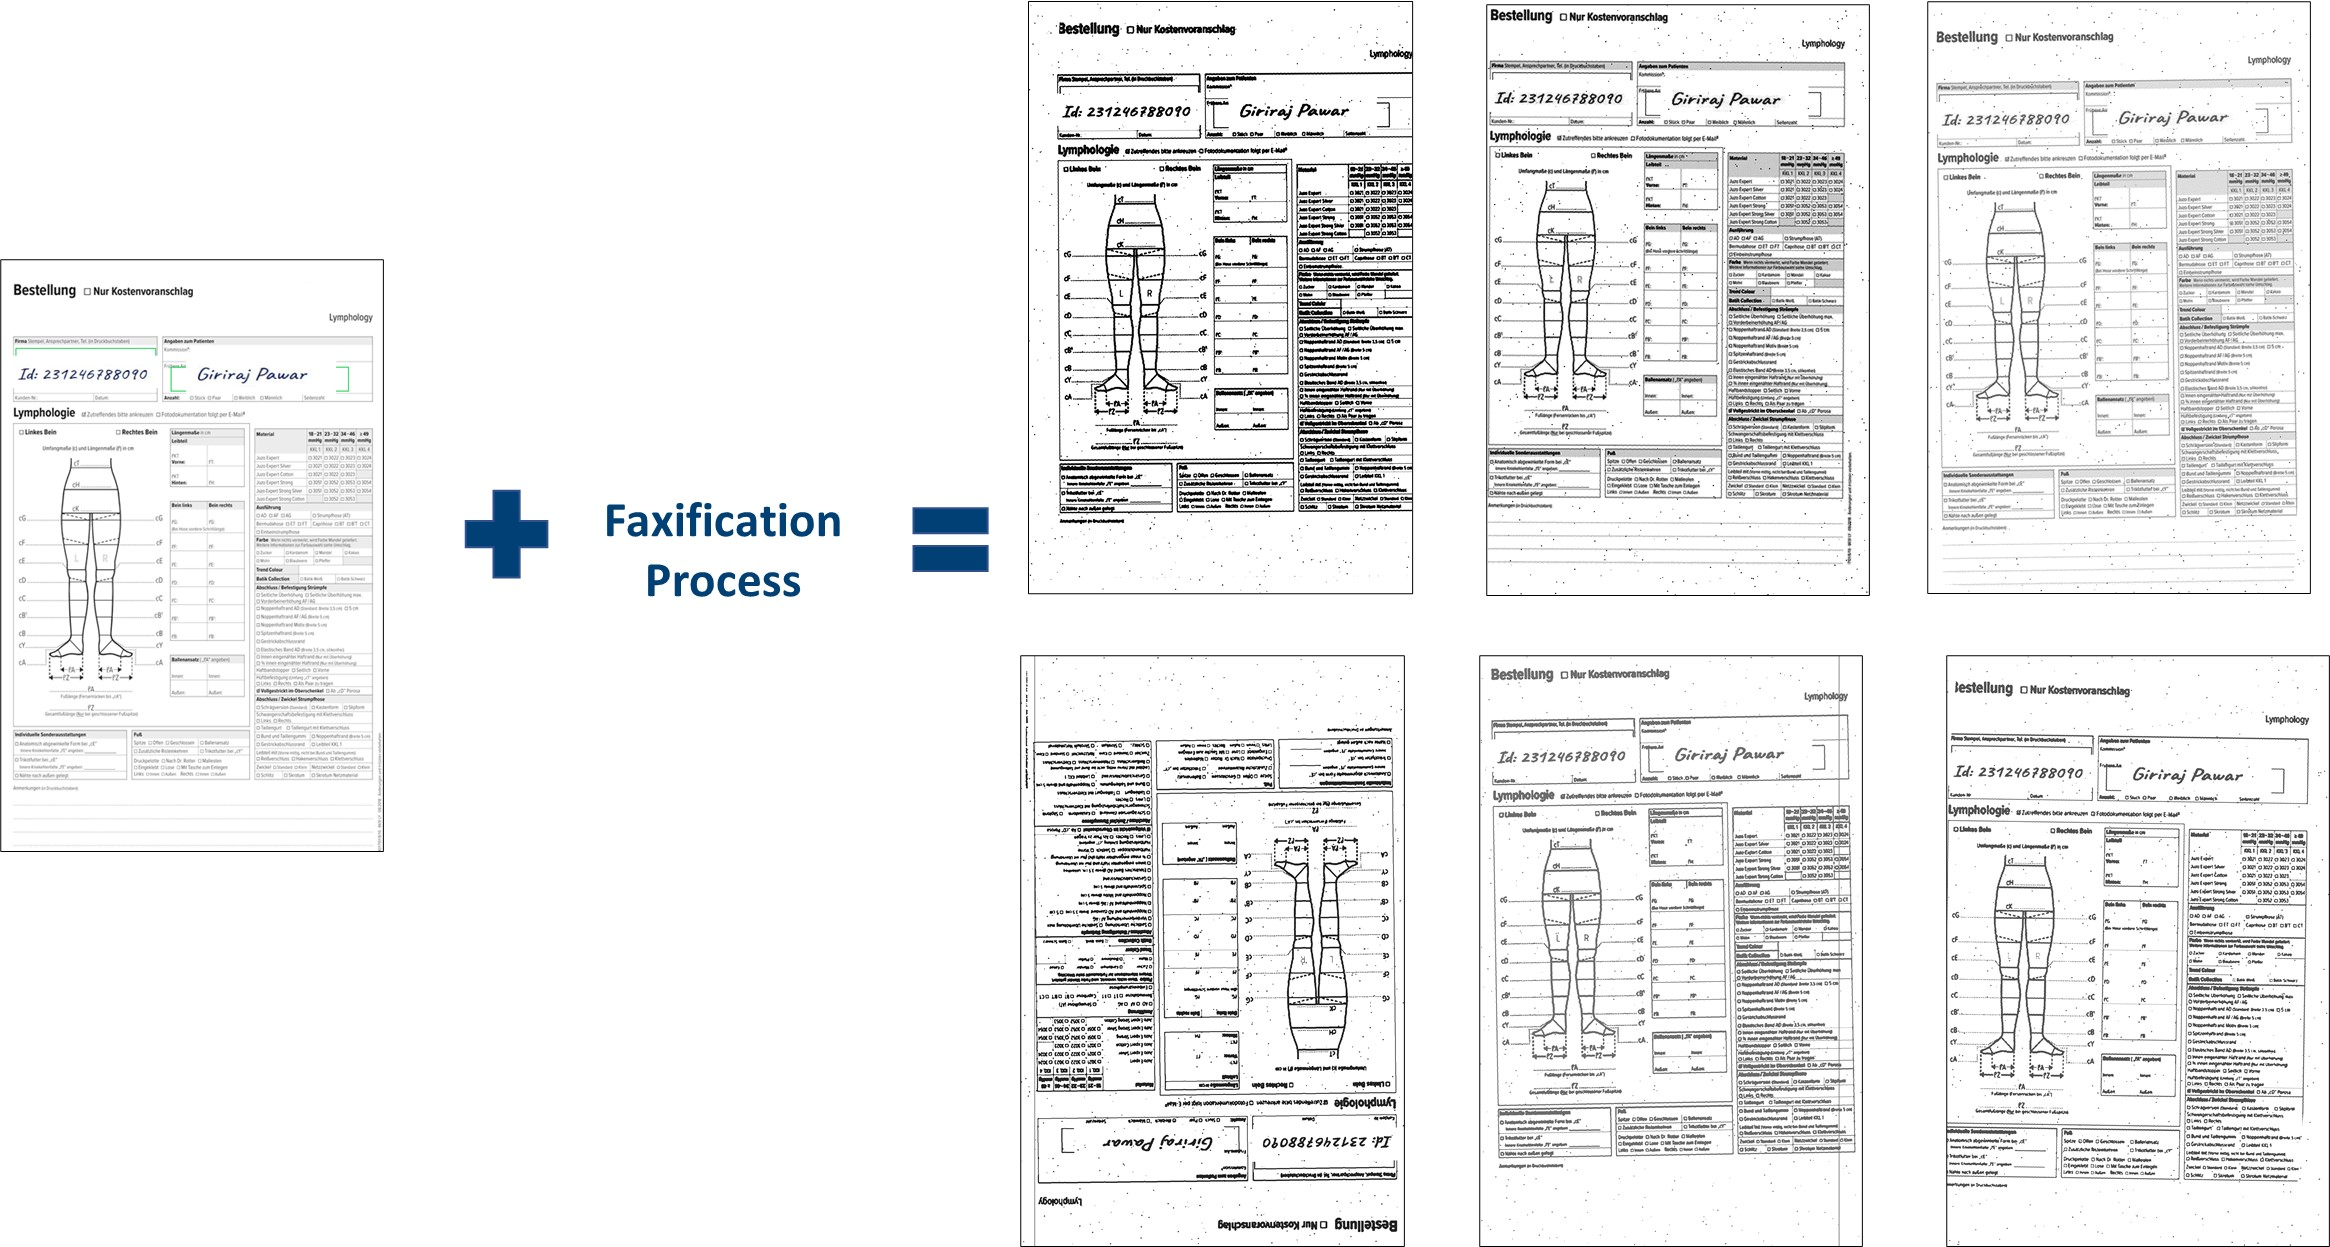
\includegraphics[scale=0.25]{images/Evaluation/FaxificationProcess.jpg}
	    \caption[An illustration of faxification process applied on synthetic document images.]{An illustration of faxification process applied on synthetic document images (figure reproduced from elevait GmbH \& Co. KG with permission).}
	    \label{fig:FaxificationProcess}
	    \end{center}
\end{figure}


\vspace*{1.5cm}
\begin{figure}[H]
        \begin{center}
	    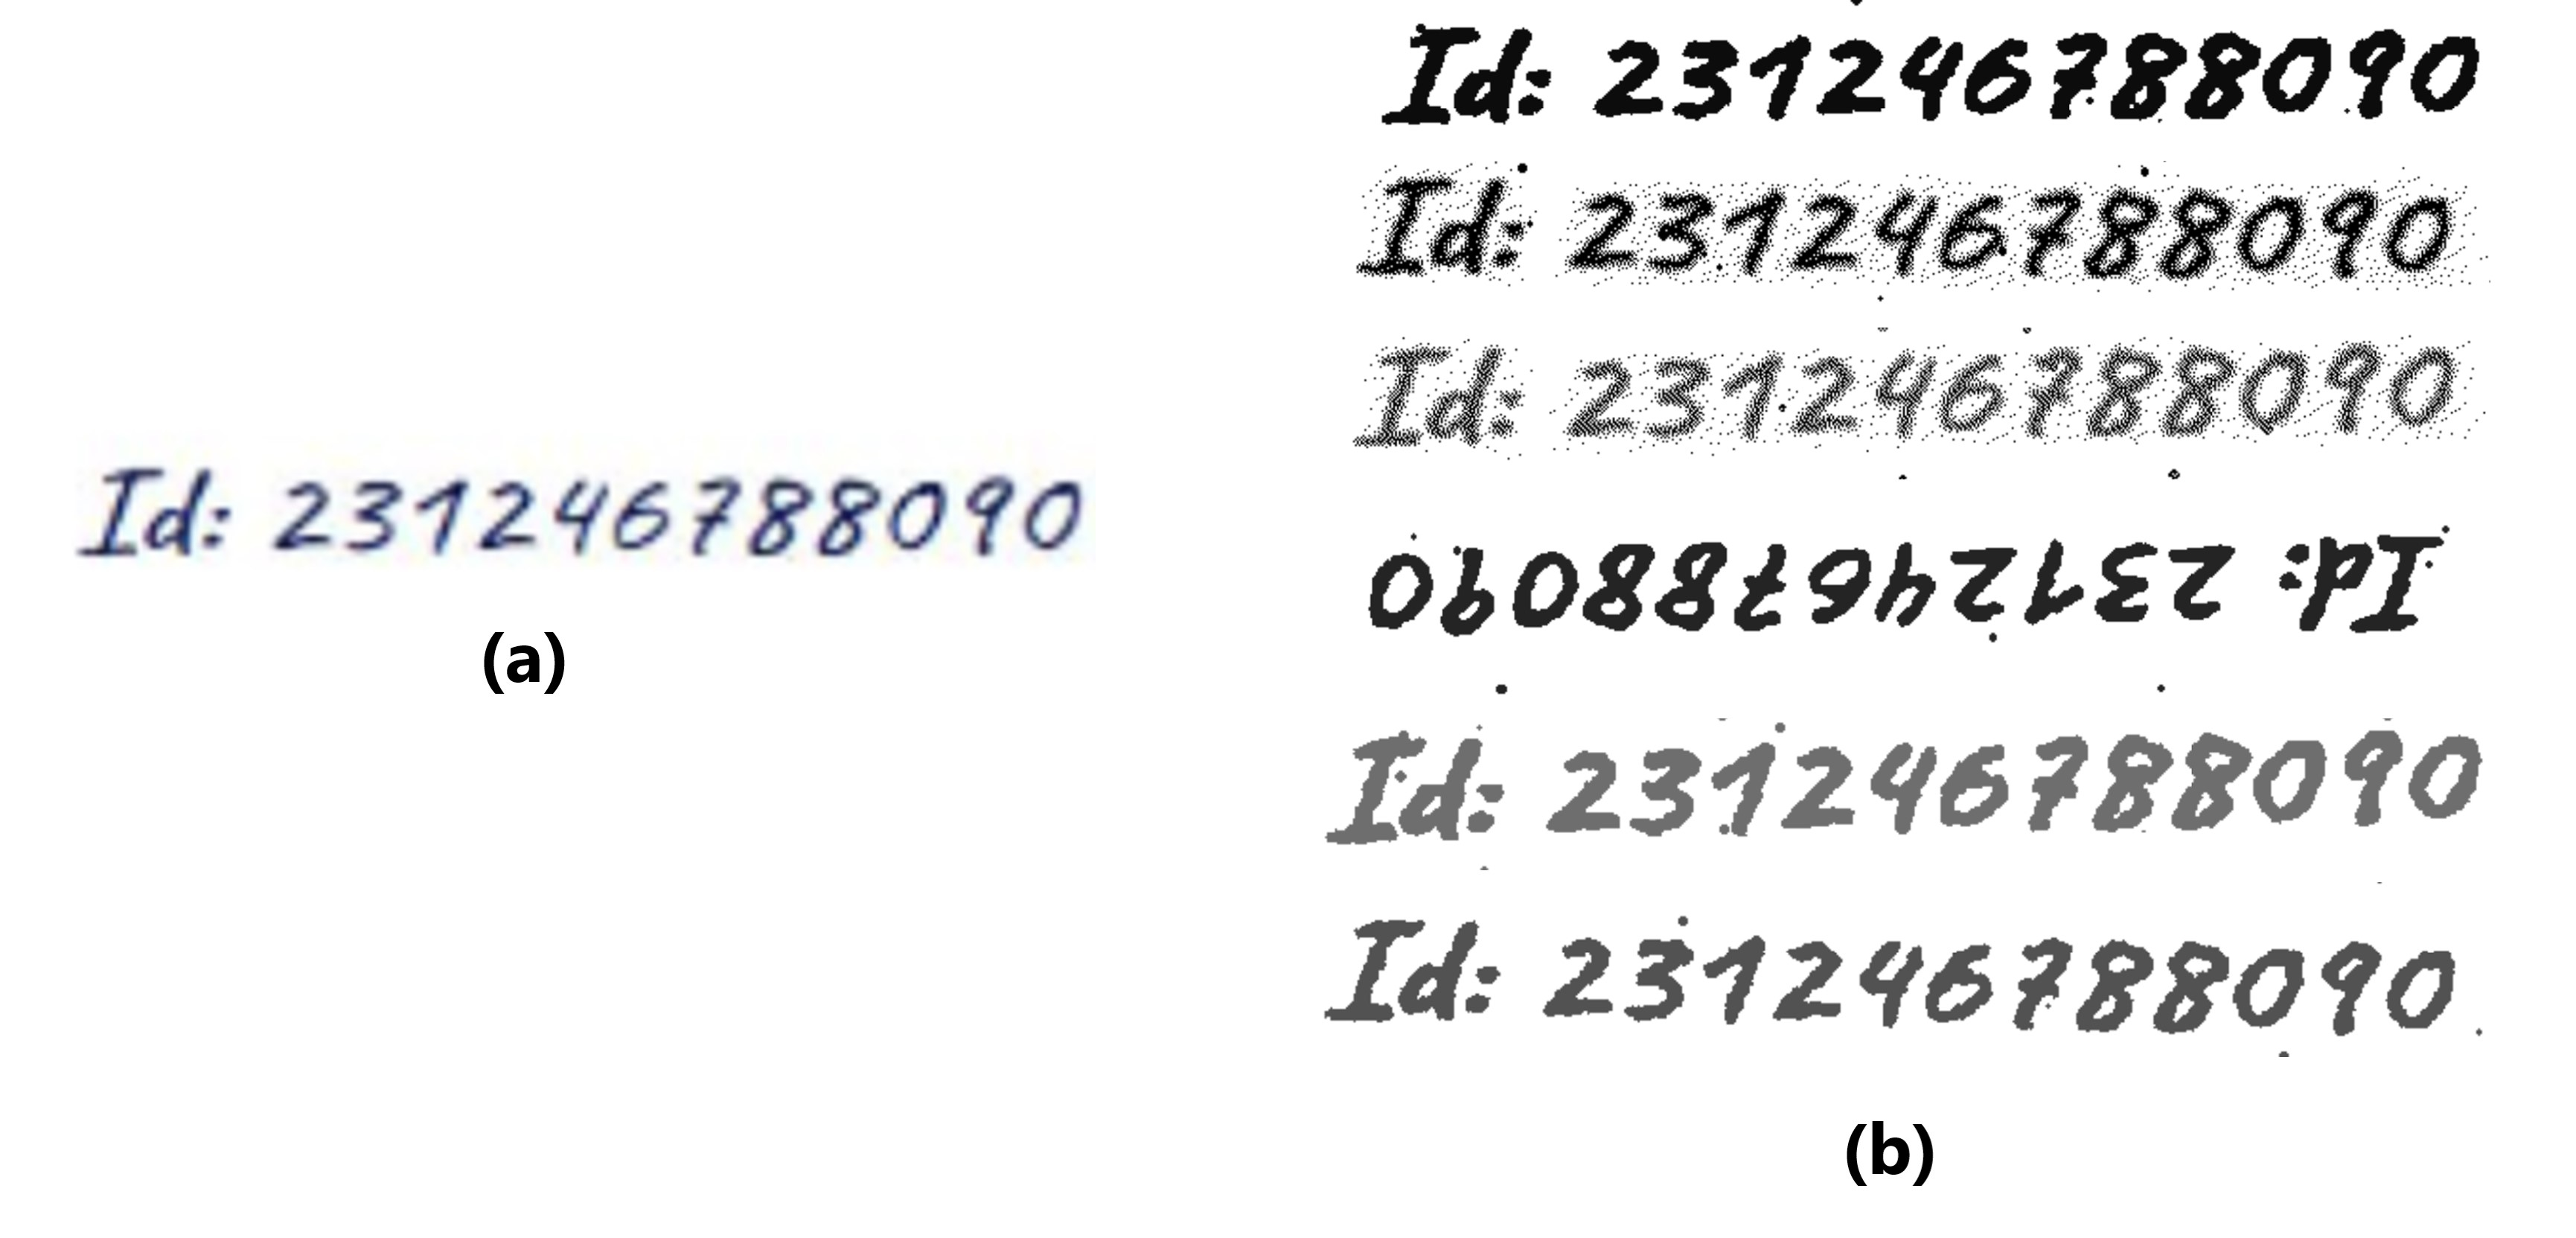
\includegraphics[scale=0.15]{images/Evaluation/FaxificationProcessZoomed.jpg}
	    \caption[An illustration of faxified document images to conclude that faxification process is a random process, the input images are faxified randomly to create distinct output.]{An illustration of faxified document images to conclude that faxification process is a random process, the input images are faxified randomly to create distinct and random output. For example, for a snippet in a synthetic document image (a), snippets of faxified document images shown in (b) are created distinct and random.}
	    \label{fig:FaxificationProcessZoomed}
	    \end{center}
\end{figure}


\vspace*{1.5cm}
\begin{figure}[H]
  \centering
  \begin{minipage}[b]{0.49\textwidth}
    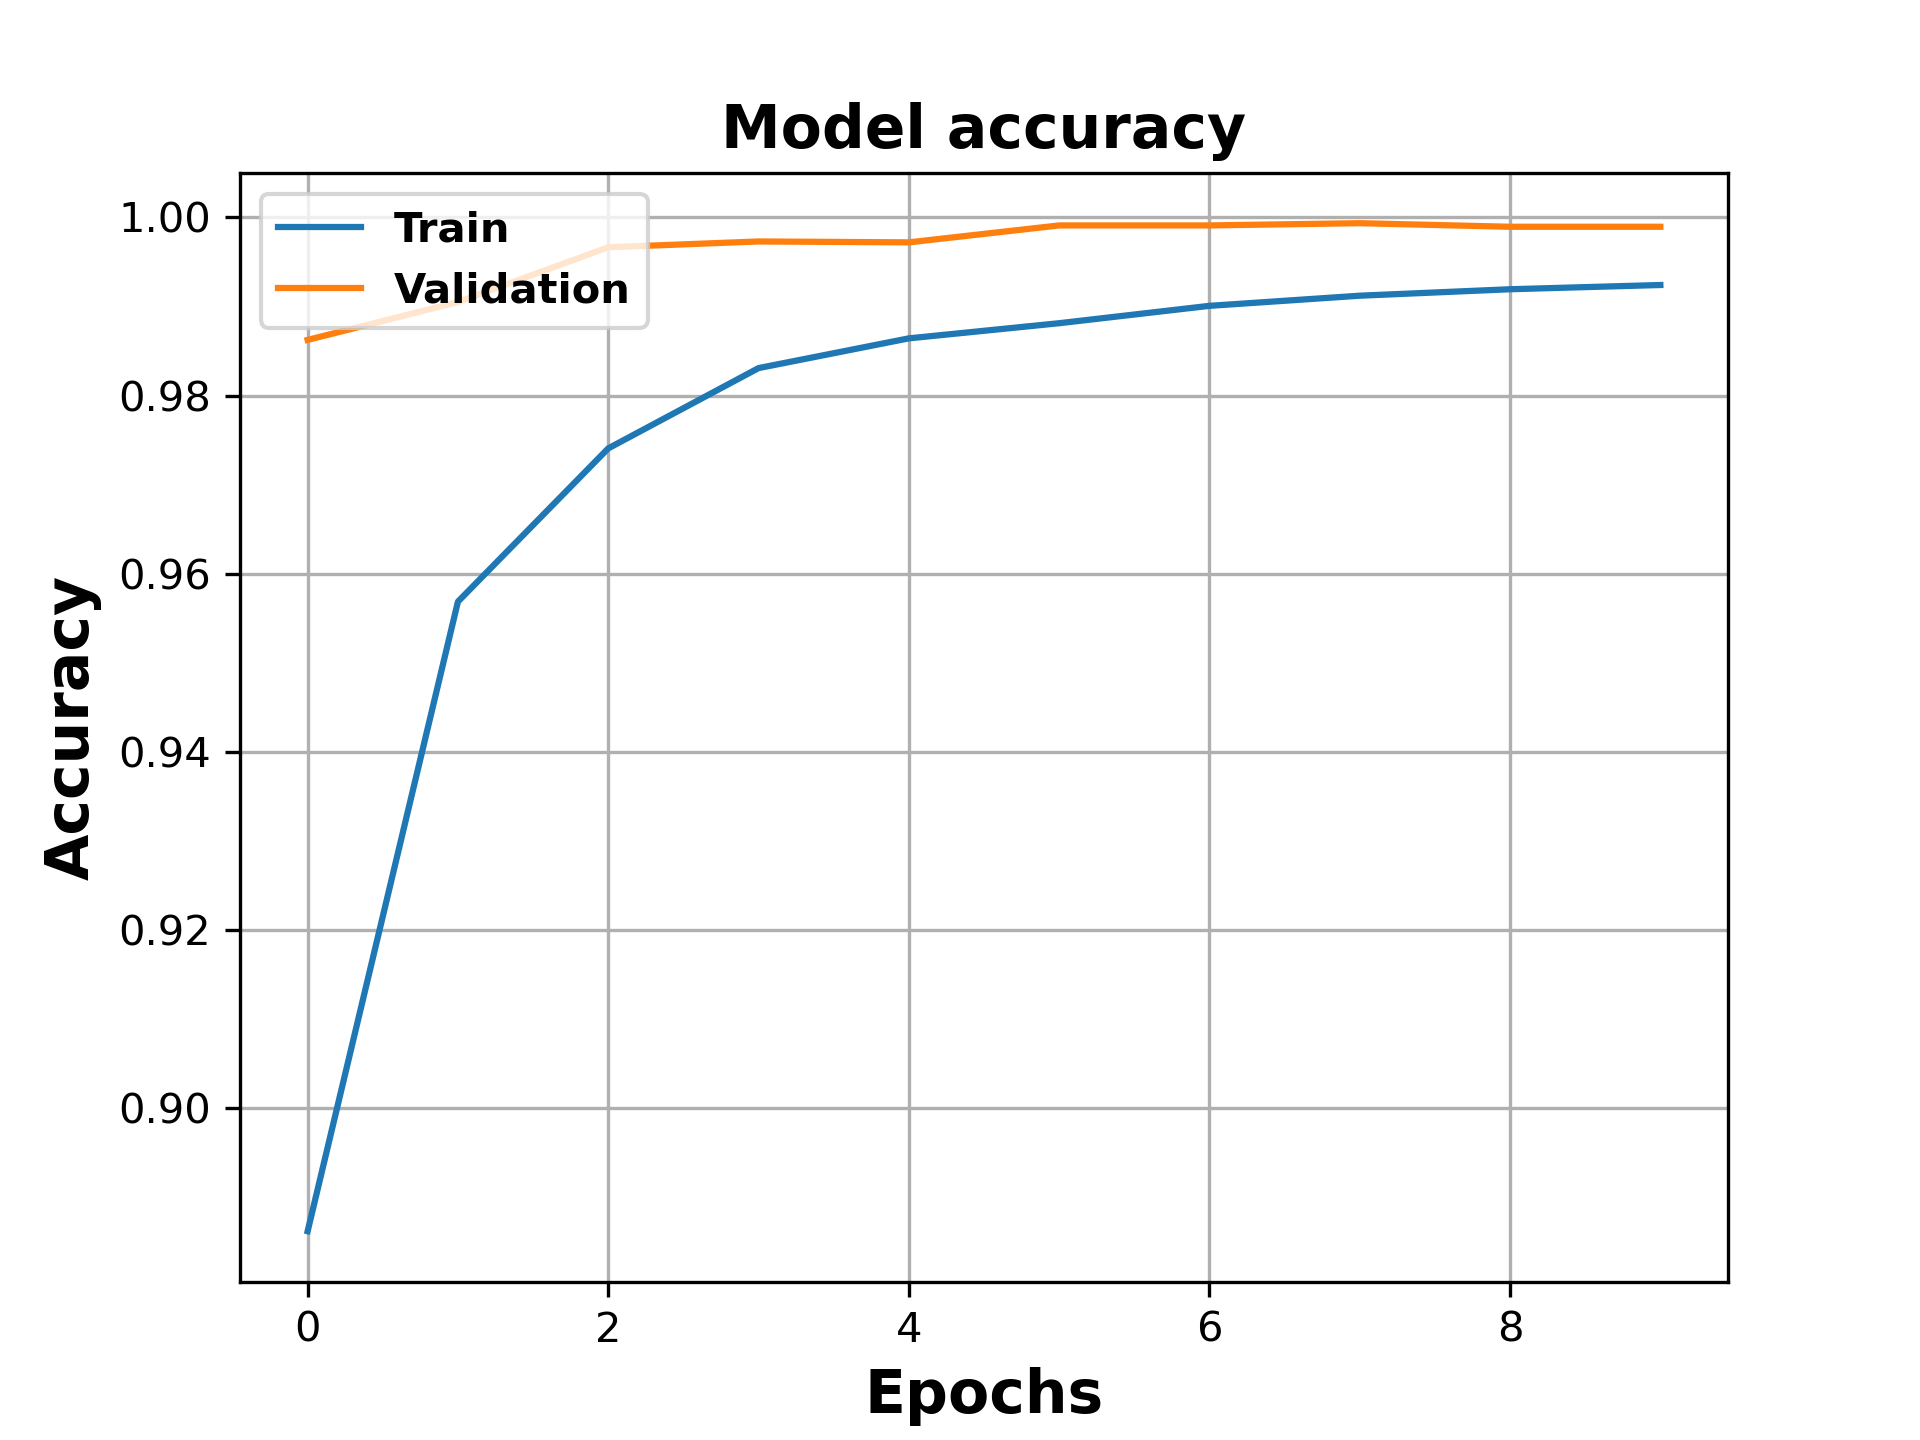
\includegraphics[width=\textwidth]{images/Evaluation/Faxified_Data_Classifier_2021-05-31_19-31-35_Accuracy.png}
    \caption[Epoch vs. Accuracy plot during training a classifier on faxified document images.]{Epoch vs. Accuracy plot during training a classifier on  faxified document images.}
    \label{fig:FaxifiedClassifierAcc}
  \end{minipage}
  \hfill
  \begin{minipage}[b]{0.49\textwidth}
    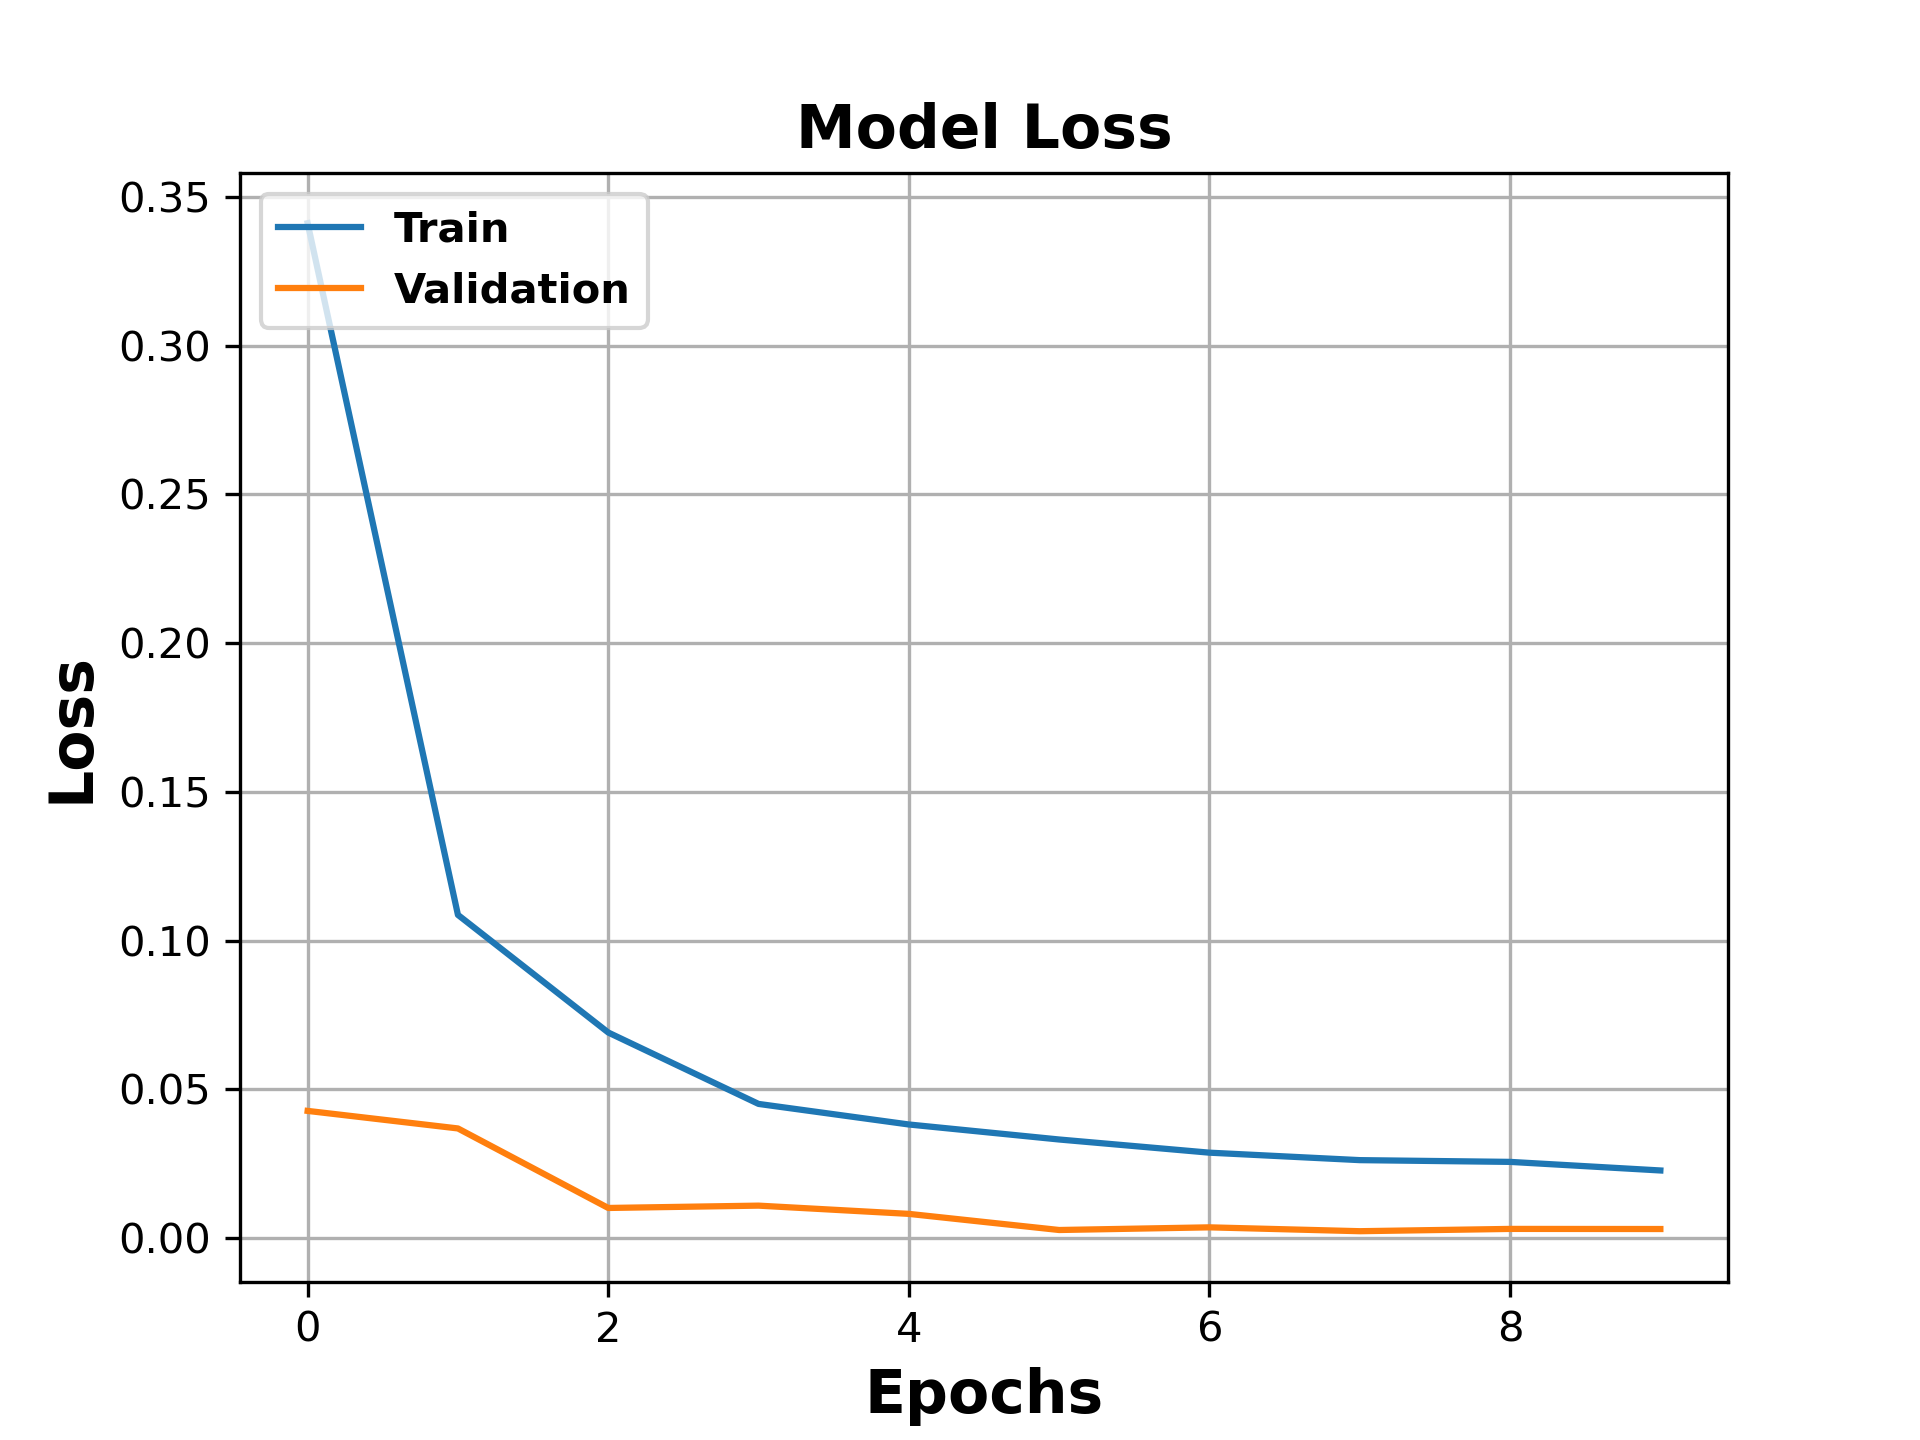
\includegraphics[width=\textwidth]{images/Evaluation/Faxified_Data_Classifier_2021-05-31_19-31-35_Loss.png}
    \caption[Epoch vs. Loss plot during training a classifier on faxified document images.]{Epoch vs. Loss plot during training a classifier on faxified document images.}
    \label{fig:FaxifiedClassifierLoss}
  \end{minipage}
\end{figure}






%Also, compared to other data distributions like synthetic and \ac{CycleGAN} generated, the faxified data distribution is more similar to the real data distribution. 


\begin{figure}[H]
    \begin{center}
	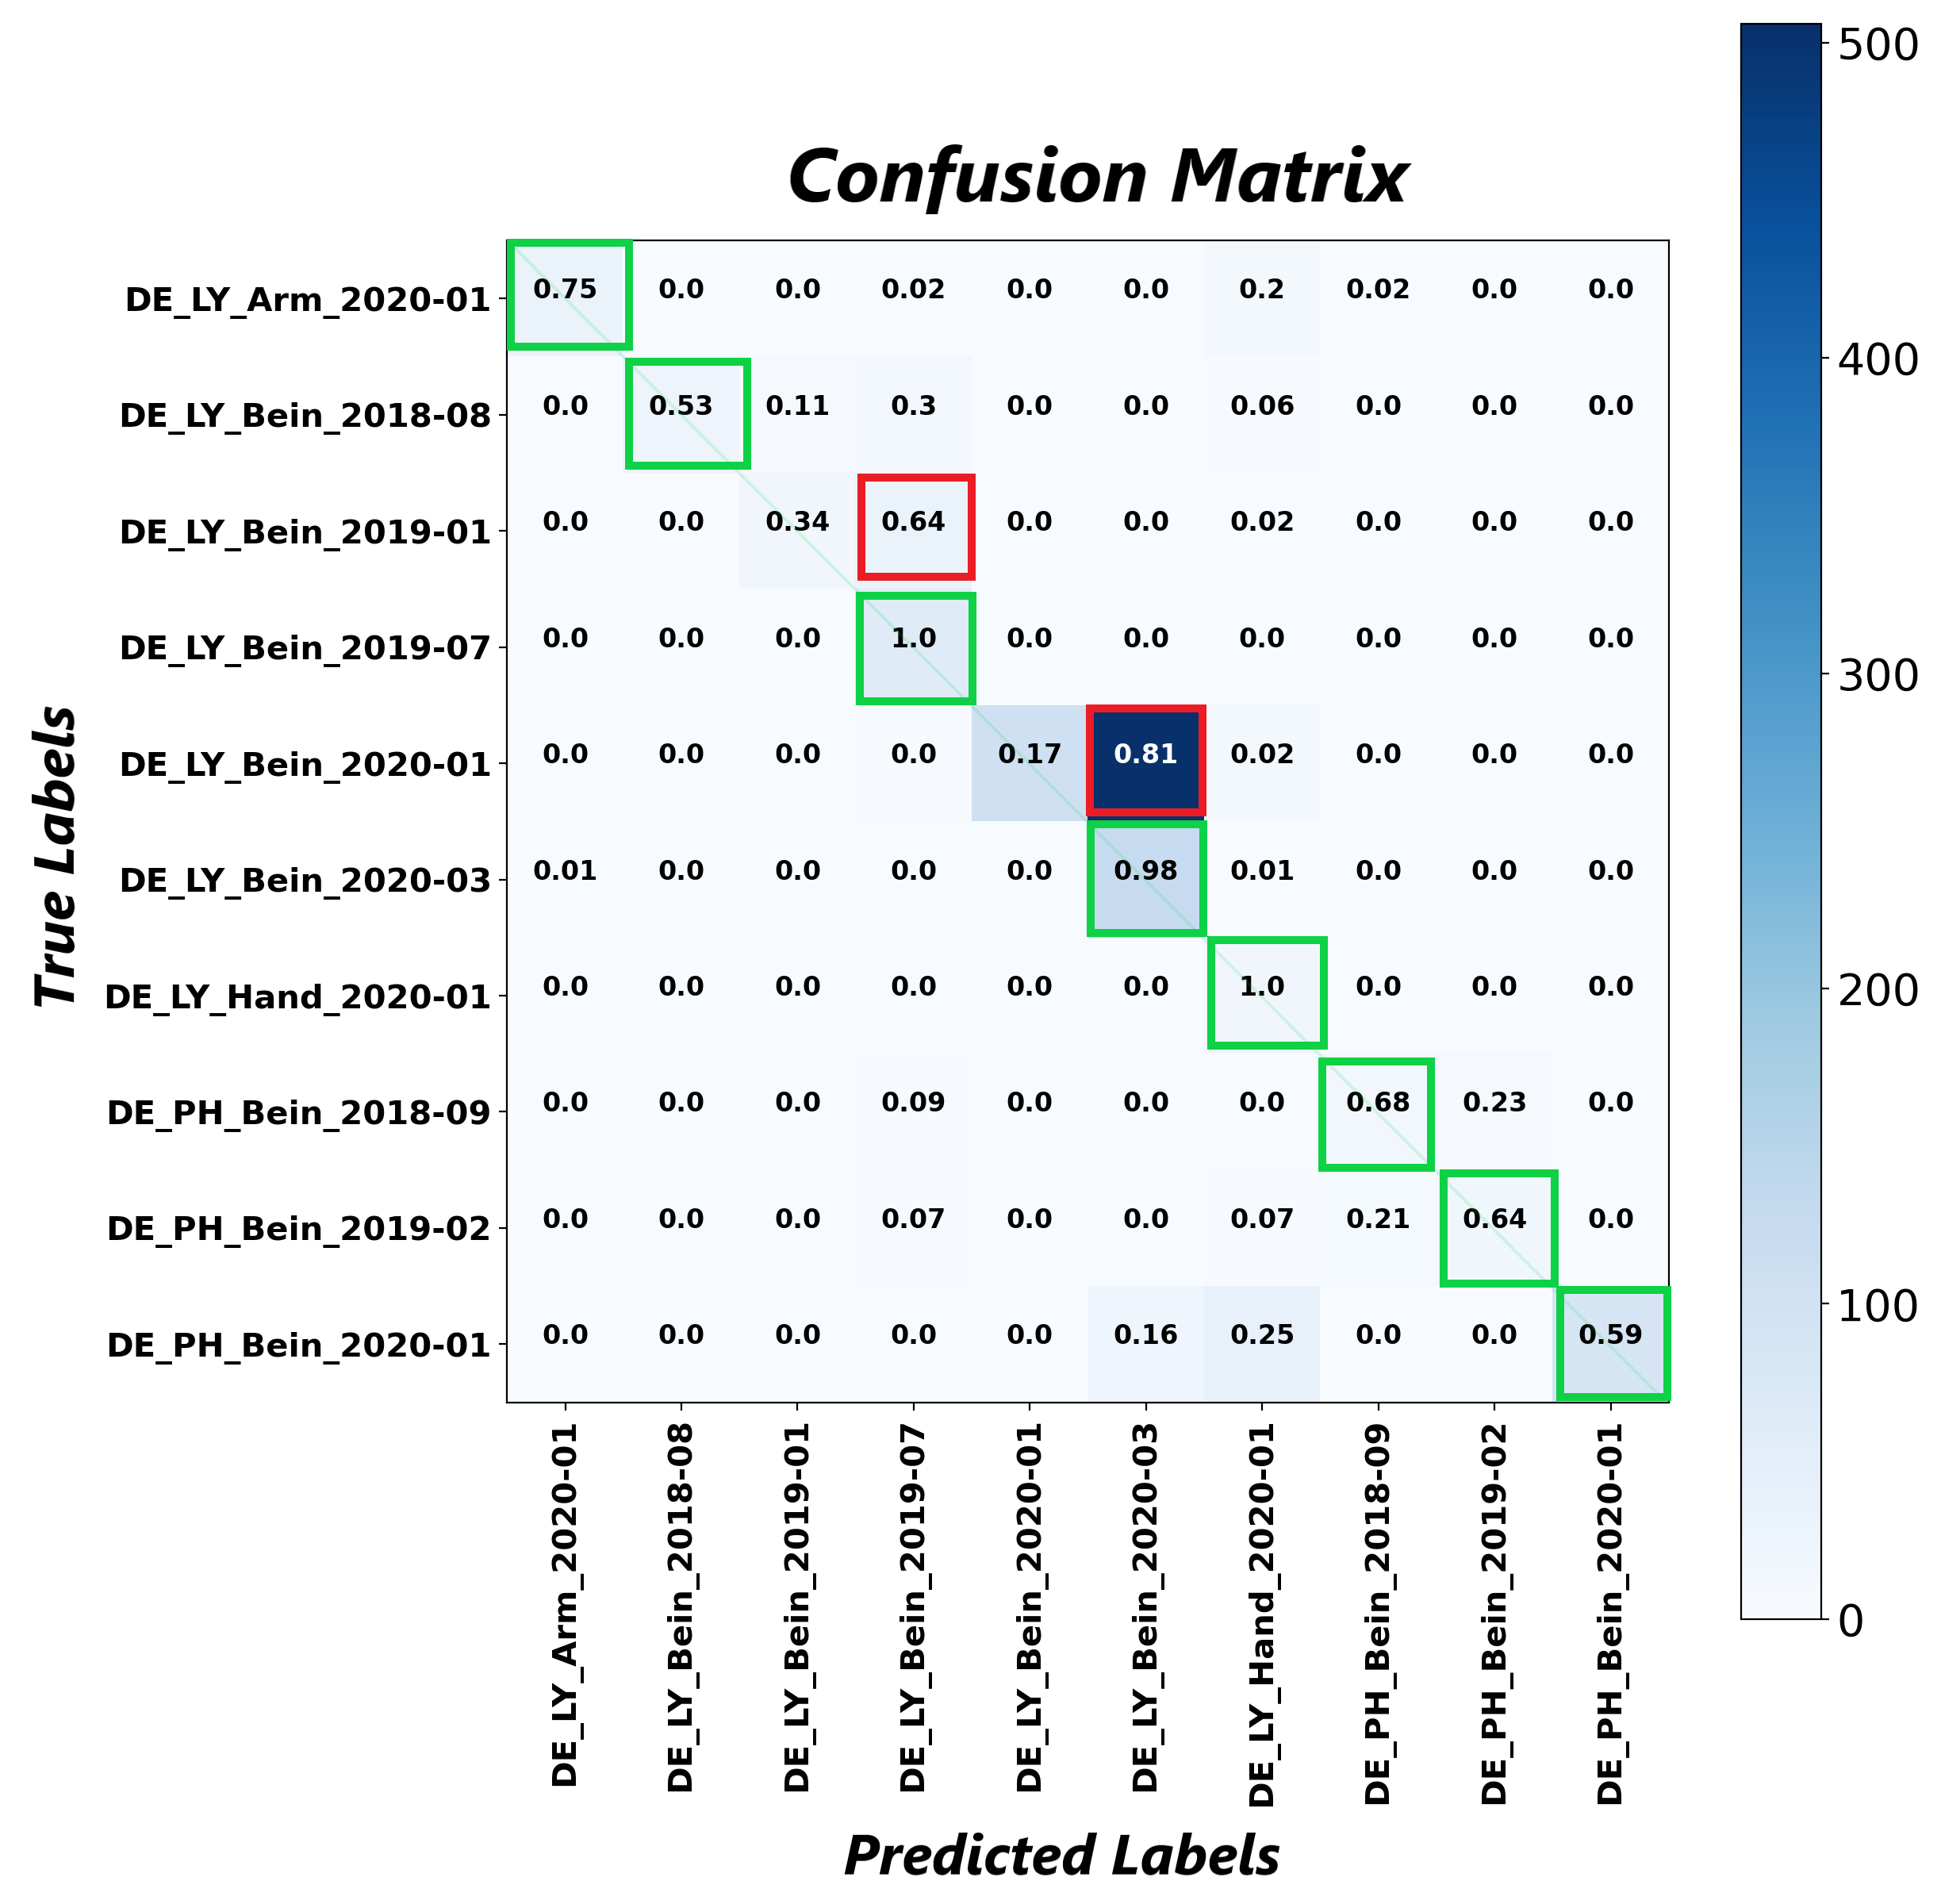
\includegraphics[scale=0.20]{images/Evaluation/Confusion_Matrix_Faxified_Data_Classifier_2021-05-31_19-31-35.png}
	\caption[Confusion matrix to analyze the performance of the classifier trained on faxified document images and evaluated using real annotated document images (test dataset).]{Confusion matrix to analyze the performance of the classifier trained on faxified document images and evaluated using real annotated document images (testing dataset). Green boxes represent classes that are correctly classified and red boxes represent classes that are misclassified.}
	\label{fig:CMFaxifiedDocumentImagesClassifier}
	\end{center}
\end{figure}

\begin{center}
\begin{table}[H]
    \begin{center}
    \begin{tabular}{P{0.22\linewidth} P{0.10\linewidth} P{0.10\linewidth} P{0.10\linewidth} P{0.10\linewidth}} 
        \toprule
            & Precision & Recall & F1-score & Support\\[0.0ex] 
        \midrule
        DE\_LY\_Arm\_2020-01 & 0.97 & 0.75 & 0.85 & 44\\[0.0ex]
        \midrule
        DE\_LY\_Bein\_2018-08 & 1.00 & 0.53 & 0.69 & 47\\[0.0ex]
        \midrule
        DE\_LY\_Bein\_2019-01 & 0.74 & 0.34 & 0.47 & 50\\[0.0ex]
        \midrule
        DE\_LY\_Bein\_2019-07 & 0.53 & 1.00 & 0.69 & 60\\[0.0ex]
        \midrule
        DE\_LY\_Bein\_2020-01 & 1.00 & 0.17 & 0.29 & 624\\[0.0ex]
        \midrule
        DE\_LY\_Bein\_2020-03 & 0.19 & 0.98 & 0.32 & 128\\[0.0ex]
        \midrule
        DE\_LY\_Hand\_2020-01 & 0.21 & 1.00 & 0.34 & 16\\[0.0ex]
        \midrule
        DE\_PH\_Bein\_2018-09 & 0.68 & 0.68 & 0.68 & 22\\[0.0ex]
        \midrule
        DE\_PH\_Bein\_2019-02 & 0.78 & 0.64 & 0.71 & 28\\[0.0ex]
        \midrule
        DE\_PH\_Bein\_2020-01 & 1.00 & 0.59 & 0.74 & 143\\[0.0ex]
        \midrule
        \midrule
        Accuracy              &      &      & \bf{0.43} & 1162\\[0.0ex]
        Macro average             & 0.71 & 0.67 & \bf{0.58} & 1162\\[0.0ex]
        Weighted average          & 0.85 & 0.43 & \bf{0.43} & 1162\\[0.0ex]

        \bottomrule
    \end{tabular}
    \caption[Classification report, evaluating a classifier on the testing dataset after training with faxified document images.]{Classification report, evaluating a classifier on the testing dataset after training with faxified document images.}
    \label{table:FaxifiedClassificationReport}
    \end{center}
\end{table}
\end{center}



\subsection{\ac{CycleGAN} Training}


%The proposed image-to-image translation application is implemented using \ac{CycleGAN}. It is trained for 20 epochs and with batch size 1. The \ac{CycleGAN} consists of two generators $G$ and $F$ and two discriminators $D_X$ and $D_Y$. The domain $X$ represents the source domain and domain $Y$ represents the target domain. The developed image-to-image translation application aims to transform synthetic document images into realistic document images. Hence, the synthetic document images represent the source domain and real document images represent the target domain. The complete architecture of the proposed image-to-image translation application using \ac{CycleGAN} is illustrated in figure \ref{fig:GxyFyx}. For more \ac{CycleGAN} training details refer section \ref{TrainingDetailsCycleGAN}. 

%The \ac{CycleGAN} training happens by calculating loss and updating the weights of discriminators $D_X$ and $D_Y$ and generators $G$ and $F$ respectively. 




The proposed image-to-image translation application is implemented using \ac{CycleGAN}. The \ac{CycleGAN} is trained using synthetic document images (Domain $X$) and real document images (Domain $Y$). The domain $X$ represents the source domain and domain $Y$ represents the target domain. The \ac{CycleGAN} consists of two generators $G$ and $F$ and two discriminators $D_X$ and $D_Y$. Further, for training, random input images $x_i$ and $y_i$ are retrieved from source domain $X$ and target domain $Y$. The fake image generated using generator $G$ is $Generated\_Y$ and the fake image generated using generator by $F$ is $Generated\_X$. As we described earlier, $G$ is a mapping function to transform an image from source domain $X$ to target domain $Y$, mathematically it is $G: X \rightarrow Y$ and $F$ is vice versa $F: Y \rightarrow X$. The generator $G$ is called the forward generator and $F$ is called the backward generator. The discriminator loss for $D_X$ and $D_Y$ on real and fake images is computed. The computed discriminator loss is used to update the weights of respective discriminator. Next, the cycle-consistency loss is calculated by transforming the source domain image into the target domain, back again into the source domain. It is called forward cycle-consistency loss. It is calculated by determining the difference between the original image in the source domain and cycled image back in the source domain. Please refer to figure \ref{fig:GxyFyx}, the forward cycle-consistency loss is the difference between \textit{Input\_X} and \textit{Cyclic\_X}. The backward cycle-consistency loss is calculated by transforming the target domain image into the source domain, back again into the target domain. In figure \ref{fig:GxyFyx}, the backward cycle-consistency loss is the difference between \textit{Input\_Y} and \textit{Cyclic\_Y}. The cycle-consistency loss forces generating an image that is context instead of generating random images.


\begin{figure}[H]
  \centering
  \begin{minipage}[b]{0.49\textwidth}
    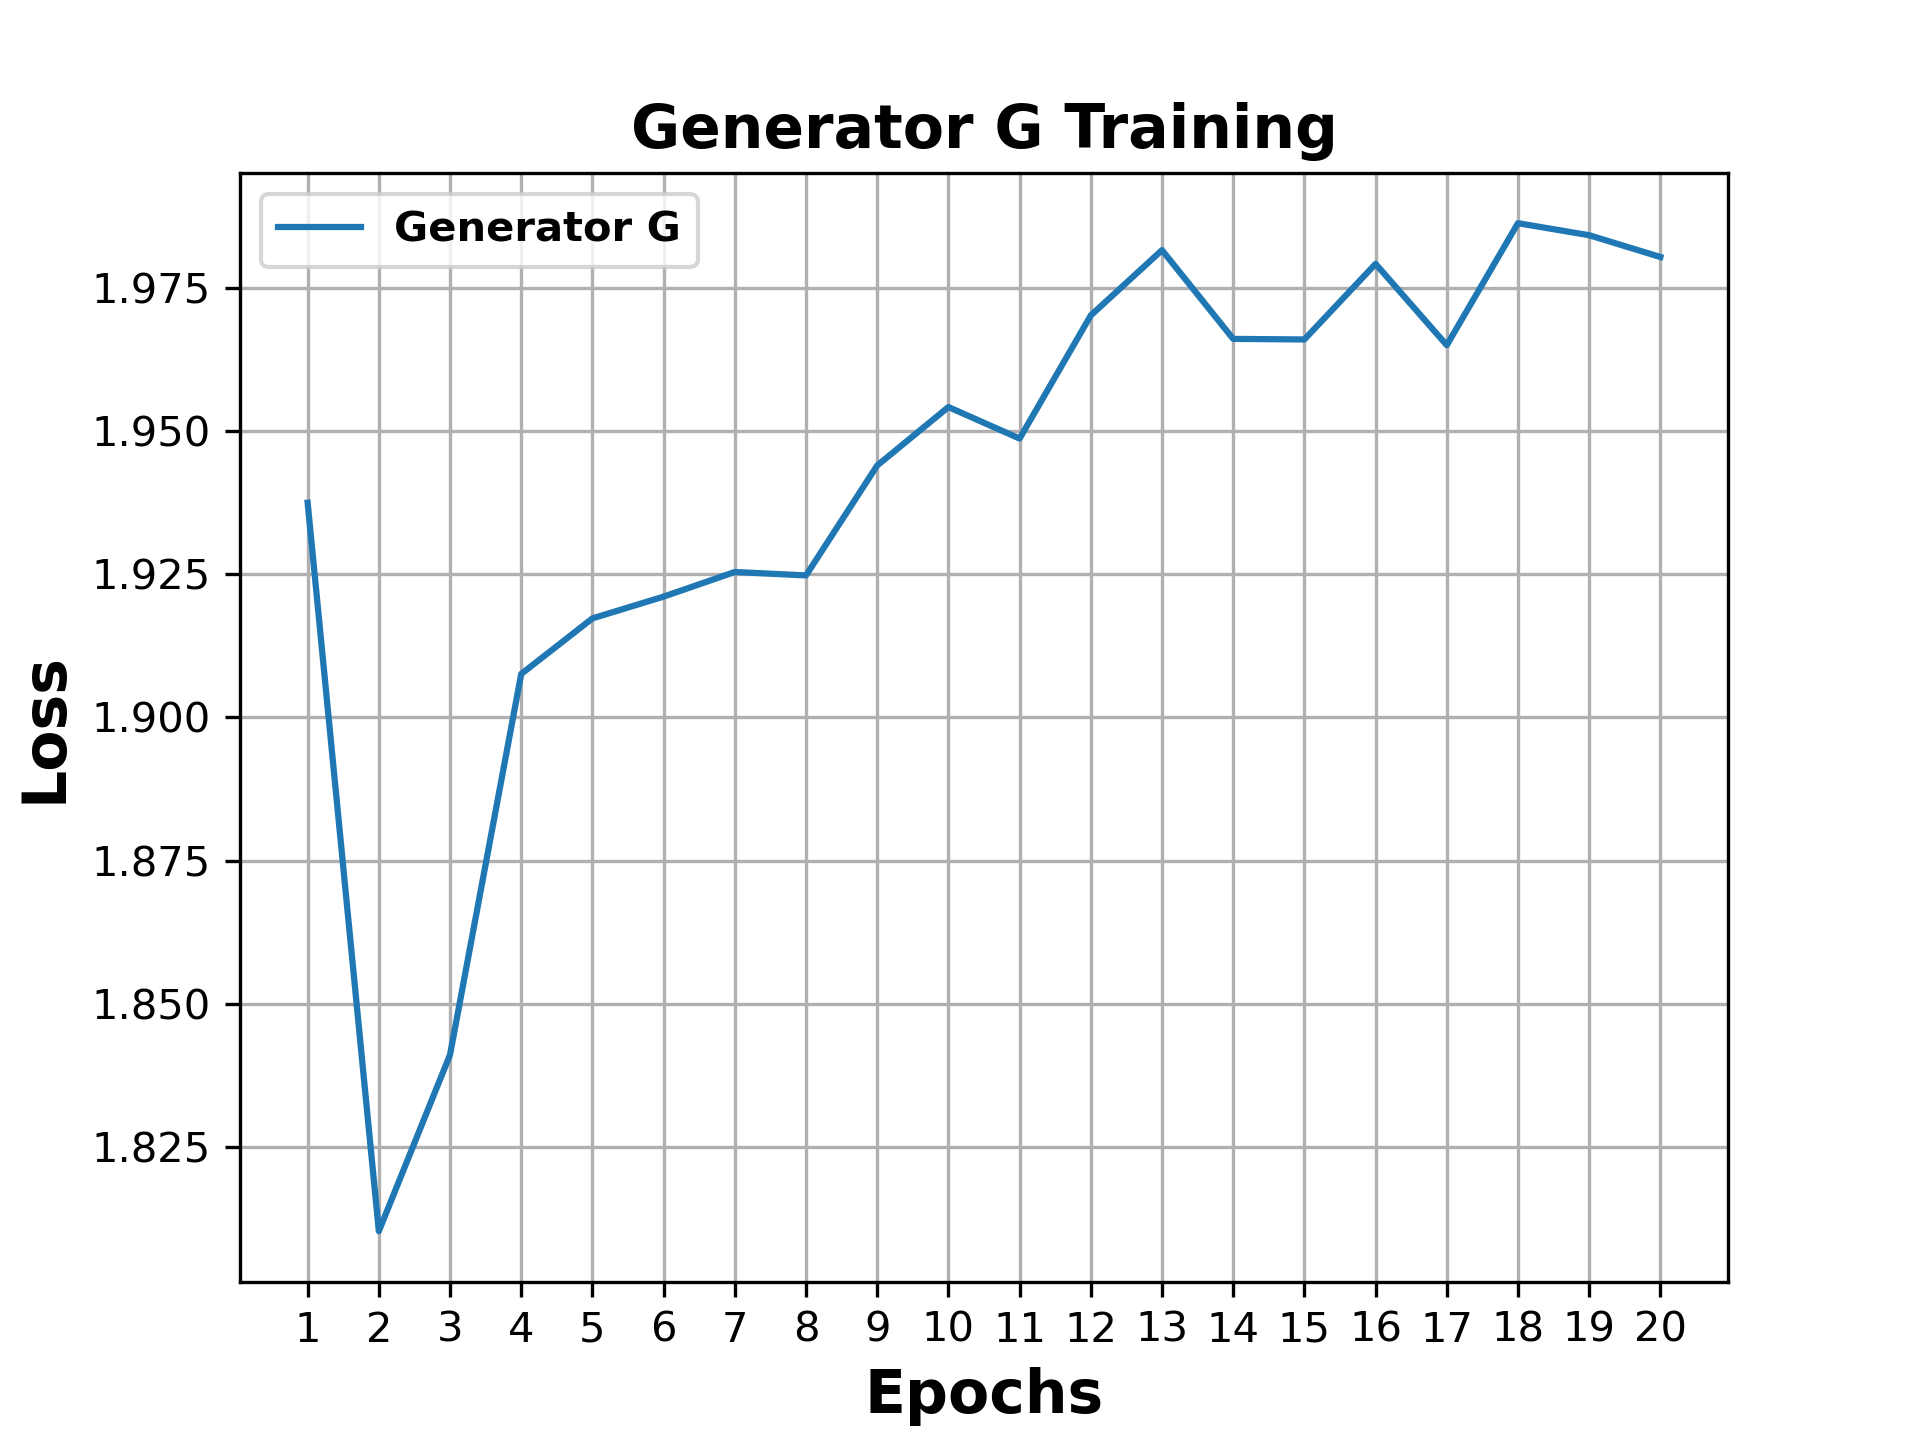
\includegraphics[width=\textwidth]{images/Evaluation/GeneratorGTraining.png}
    \caption[Epochs vs. Loss plot during Generator $G$ is training.]{Epochs vs. Loss plot during Generator $G$ is training.}
    \label{fig:generatorG}
  \end{minipage}
  \hfill
  \begin{minipage}[b]{0.49\textwidth}
    \includegraphics[width=\textwidth]{images/Evaluation/DiscriminatorDyTraining.png}
    \caption[Epochs vs. Loss plot during Discriminator $D_Y$ is training.]{Epochs vs. Loss plot during Discriminator $D_Y$ is training.}
    \label{fig:discriminatorDy}
  \end{minipage}
\end{figure}
vspace*{0.1cm}
\begin{figure}[H]
  \centering
  \begin{minipage}[b]{0.49\textwidth}
    \includegraphics[width=\textwidth]{images/Evaluation/GeneratorFTraining.png}
    \caption[Epochs vs. Loss plot during Generator $F$ is training.]{Epochs vs. Loss plot during Generator $F$ is training.}
    \label{fig:generatorF}
  \end{minipage}
  \hfill
  \begin{minipage}[b]{0.49\textwidth}
    \includegraphics[width=\textwidth]{images/Evaluation/DiscriminatorDxTraining.png}
    \caption[Epochs vs. Loss plot during Discriminator $D_X$ is training.]{Epochs vs. Loss plot during Discriminator $D_X$ is training.}
    \label{fig:discriminatorDx}
  \end{minipage}
\end{figure}


Further, identity mapping loss is calculated to preserve the color of images after domain translation using generators $G$ and $F$. The generator $G$ transforms the image from domain $X$ to the domain $Y$. When the input $y_i$ is given to generator $G$ from the target domain $Y$, it should produce an identical image. The identity mapping loss for generator $G$ is the difference between the original image $y_i$ and the transformed image \textit{Same\_Y} when $y_i$ is used as an input for $G$. And, the identity mapping loss for generator $F$ is the difference between input image $x_i$ and the transformed image \textit{Same\_X} when $x_i$ is used as an input for $F$. The generator loss for generators $G$ and $F$ is calculated by the feedback given by their respective discriminators $D_Y$ and $D_X$. Combining generator loss, cycle-consistency loss and identity mapping loss, the total generator loss is calculated separately for generators $G$ and $F$ and their weights are updated to produce quality images. The epochs against loss plot while training generators $G$ and $F$ are shown in figure \ref{fig:generatorG} and \ref{fig:generatorF} respectively. Also, the epochs against loss plot while training discriminators $D_Y$ and $D_X$ are shown in figure \ref{fig:discriminatorDy} and \ref{fig:discriminatorDx} respectively. The algorithm of \ac{CycleGAN} is described in section \ref{CycleGANAlgorithm}. The complete architecture of the proposed image-to-image translation application using \ac{CycleGAN} is illustrated in figure \ref{fig:GxyFyx}. For more \ac{CycleGAN} training details refer section \ref{TrainingDetailsCycleGAN}. 




\subsection{Training a Classifier on \ac{CycleGAN} Generated Document Images}\label{trainingCycleGANDataClassifier}


Once \ac{CycleGAN} is trained, the generator $G$ is retrieved from the saved \ac{CycleGAN} model to transform synthetic document images to realistic document images. 100,000 synthetic document images are transformed into realistic document images. The classifier is trained using these transformed 100,000 realistic document images. The performance of this classifier is evaluated on the testing dataset (Annotated real document images) to understand the domain gap between real data distribution and \ac{CycleGAN} generated data distribution. The purpose of this experiment is to determine how closely the \ac{CycleGAN} generated data distribution matches the real data distribution. The quality of generated realistic document images can be determined using this experiment. The classification report in table \ref{table:CycleGANClassificationReport} states that the accuracy of this classifier on the testing dataset is 27\%, macro average F1-score is 34\% and weighted average F1-score is 25\%. 


The results conclude that the faxified data distribution matched the real data distribution better than the \ac{CycleGAN} generated data distribution. The confusion matrix is illustrated in figure \ref{fig:CMFaxifiedDocumentImagesClassifier}. In which, the document images DE\_LY\_Arm\_2020-01 (support 44 and recall 75\%), DE\_LY\_Bein\_2019-07 (support 60 and recall 83\%), DE\_LY\_Hand\_2020-01 (support 16 and recall 75\%), DE\_PH\_Bein\_2019-02 (support 28 and recall 46\%) and DE\_PH\_Bein\_2020-01 (support 143 and recall 67\%) are classified satisfactorily, with convincing recall score. Document images DE\_LY\_Bein\_2020-01 and DE\_LY\_Bein\_2020-03 are wrongly classified as DE\_LY\_Bein\_2019-07. Document images DE\_PH\_Bein\_2018-09 and DE\_PH\_Bein\_2019-02 are wrongly classified as DE\_PH\_Bein\_2019-02. As shown in the in confusion matrix \ref{fig:CMCycleganGeneratedDocumentImagesClassifier}, most of the generated document images DE\_LY\_Bein\_2019-01 are misclassified as DE\_LY\_Bein\_2019-07. The real document images DE\_LY\_Bein\_2019-01 and DE\_LY\_Bein\_2019-07 are similar to each other with couple of minor differences. Examples of DE\_LY\_Bein\_2019-01 and DE\_LY\_Bein\_2019-07 real document images are illustrated in figure \ref{fig:MissclassificationExample}. It is challenging for \ac{CycleGAN} to learn such minor differences and features from large training datasets. Also, the majority of document images are of the type ``Bein'' and they are similar to each other, learning minor differences and features between them from the training dataset is very challenging. The \ac{CycleGAN} is failed to learn such small and complex differences, hence some of the generated images are more similar to different classes than the original class and they are misclassified. In section \ref{QualitativeResults}, qualitative results of the image-to-image translation are illustrated along with failure cases. The epochs against accuracy and epochs against loss plots while training classifier on \ac{CycleGAN} generated document images is illustrated in figure \ref{fig:CycleGANClassifierAcc} and \ref{fig:CycleGANClassifierLoss} respectively.


\begin{figure}[H]
  \centering
  \begin{minipage}[b]{0.45\textwidth}
    \includegraphics[width=\textwidth]{images/Evaluation/CycleGAN_Generated_Data_Classifier_2021-06-02_21-55-39_Accuracy.png}
    \caption[Epochs vs. Accuracy plot during training a classifier on \ac{CycleGAN} generated document images.]{Epochs vs. Accuracy plot during training a classifier  on \ac{CycleGAN} generated document images.}
    \label{fig:CycleGANClassifierAcc}
  \end{minipage}
  \hfill
  \begin{minipage}[b]{0.45\textwidth}
    \includegraphics[width=\textwidth]{images/Evaluation/CycleGAN_Generated_Data_Classifier_2021-06-02_21-55-39_Loss.png}
    \caption[Epochs vs. Loss plot during training a classifier on \ac{CycleGAN} generated document images.]{Epochs vs. Loss plot during training a classifier on \ac{CycleGAN} generated document images.}
    \label{fig:CycleGANClassifierLoss}
  \end{minipage}
\end{figure}


\begin{figure}[H]
    \begin{center}
	\includegraphics[scale=0.20]{images/Evaluation/Confusion_Matrix_CycleGAN_Generated_Data_Classifier_2021-06-02_21-55-39.png}
	\caption[Confusion matrix to analyze the performance of the classifier trained on \ac{CycleGAN} generated document images and evaluated using real annotated document images (test dataset).]{Confusion matrix to analyze the performance of the classifier trained on \ac{CycleGAN} generated document images and evaluated using real annotated document images (testing dataset). Green boxes represent classes that are correctly classified and red boxes represent classes that are misclassified.}
	\label{fig:CMCycleganGeneratedDocumentImagesClassifier}
	\end{center}
\end{figure}

\begin{center}
\begin{table}[H]
    \begin{center}
    \begin{tabular}{P{0.22\linewidth} P{0.10\linewidth} P{0.10\linewidth} P{0.10\linewidth} P{0.10\linewidth}} 
	        \toprule
            & Precision & Recall & F1-score & Support\\[0.0ex] 
        \midrule
        DE\_LY\_Arm\_2020-01 & 0.53 & 0.75 & 0.62 & 44\\[0.0ex]
        \midrule
        DE\_LY\_Bein\_2018-08 & 0.21 & 0.28 & 0.24 & 47\\[0.0ex]
        \midrule
        DE\_LY\_Bein\_2019-01 & 0.16 & 0.14 & 0.15 & 50\\[0.0ex]
        \midrule
        DE\_LY\_Bein\_2019-07 & 0.11 & 0.83 & 0.19 & 60\\[0.0ex]
        \midrule
        DE\_LY\_Bein\_2020-01 & 0.72 & 0.07 & 0.12 & 624\\[0.0ex]
        \midrule
        DE\_LY\_Bein\_2020-03 & 0.16 & 0.34 & 0.22 & 128\\[0.0ex]
        \midrule
        DE\_LY\_Hand\_2020-01 & 0.80 & 0.75 & 0.77 & 16\\[0.0ex]
        \midrule
        DE\_PH\_Bein\_2018-09 & 0.07 & 0.05 & 0.06 & 22\\[0.0ex]
        \midrule
        DE\_PH\_Bein\_2019-02 & 0.33 & 0.46 & 0.39 & 28\\[0.0ex]
        \midrule
        DE\_PH\_Bein\_2020-01 & 0.70 & 0.67 & 0.68 & 143\\[0.0ex]
        \midrule
        \midrule
        Accuracy              &      &      & \bf{0.27} & 1162\\[0.0ex]
        Macro average             & 0.38 & 0.43 &  \bf{0.34} & 1162\\[0.0ex]
        Weighted average          & 0.55 & 0.27 &  \bf{0.25} & 1162\\[0.0ex]
        \bottomrule
    \end{tabular}
    \caption[Classification report, evaluating a classifier on the testing dataset after training with \ac{CycleGAN} generated document images.]{Classification report, evaluating a classifier on the testing dataset after training with \ac{CycleGAN} generated document images.}
    \label{table:CycleGANClassificationReport}
    \end{center}
\end{table}
\end{center}

\vspace*{2cm}

\begin{figure}[H]
    \begin{center}
	\includegraphics[scale=0.50]{images/Evaluation/MissclassificationExample.png}
	\caption[Examples of DE\_LY\_Bein\_2019-01 and DE\_LY\_Bein\_2019-07 real document images.]{Examples of DE\_LY\_Bein\_2019-01 and DE\_LY\_Bein\_2019-07 real document images. Both real document images are similar to each other hence learning such minor differences from the training dataset is a challenging for \ac{CycleGAN}.}
	\label{fig:MissclassificationExample}
	\end{center}
\end{figure}


\newpage
\section{Results}\label{results}

This section discusses the qualitative and quantitative results of the proposed image-to-image translation application implemented using \ac{CycleGAN}. In experiments, three separate classifiers are trained on three data distributions, synthetic data distribution, faxified data distribution and \ac{CycleGAN} generated data distribution. The performance of these classifiers that are trained using different distributions is evaluated and compared using the testing dataset (Annotated real document images) to analyze the domain gap between these distributions and real data distribution. The experiment of training a classifier on \ac{CycleGAN} generated document images and evaluating on testing dataset helps to determine the quality of \ac{CycleGAN} generated document images. It shows how close the generated document images are to the real document images.

The performance of the classifiers is evaluated using metrics like accuracy, macro average F1-score and weighted average F1-score. The accuracy of a classifier trained on synthetic document images is 25\%, the accuracy of a classifier trained on faxified document images is 27\% and the accuracy of a classifier trained on \ac{CycleGAN} generated document images is 43\%. The accuracy is not a suitable metric to evaluate the performance of the classifiers when imbalanced datasets are involved\footnote{\url{https://machinelearningmastery.com/failure-of-accuracy-for-imbalanced-class-distributions/} \dcdate}. The performance evaluation of the classifiers trained on different data distributions is calculated using an imbalanced testing dataset. Hence, it will be beneficial to consider macro average and weighted average F1-score metrics to evaluate the performance of the classifiers. The macro average F1-score of a classifier trained on synthetic document images is 27\%, the macro average F1-score of a classifier trained on faxified document images is 34\% and the macro average F1-score of a classifier trained on \ac{CycleGAN} generated document images is 58\%. The weighted average F1-score states, 25\% real document images were correctly classified when a classifier is trained using \ac{CycleGAN} generated document images. 43\% real document images were correctly classified when a classifier is trained using faxified document images. 31\% real document images were correctly classified when a classifier is trained using synthetic document images. Finally, results conclude that the quantitatively \ac{CycleGAN} generated data distribution could not match real data distribution thoroughly. The faxified data distribution produced by faxifying synthetic document images convincingly matched the real data distribution, therefore, the faxified document images are more similar to the real document images compared to \ac{CycleGAN} generated document images. The quantitative results are illustrated using a table and bar plot in section \ref{QuantitativeResults}. The proposed image-to-image translation application can be improved further in the future using different methods and loss functions. The future work and conclusion are discussed in the chapter \ref{conclusion}.


\subsection{Quantitative Evaluation}\label{QuantitativeResults}


\begin{table}[H]
\begin{tabular}{P{0.25\linewidth} P{0.20\linewidth} P{0.20\linewidth} P{0.20\linewidth}} 
	\toprule
	\bf{Data distributions} & \bf{Accuracy}  & \bf{Macro average F1-score} & \bf{Weighted average F1-score}\\[0.0ex] 
	\midrule
     \bf{Synthetic document images} & 25\% & 27\% & 31\%\\[0.0ex]
     \midrule
     \bf{\ac{CycleGAN} generated document images} & 27\% & 34\% & 25\%\\[0.0ex]
     \midrule
     \bf{Faxified document images} & 43\% & 58\% & 43\%\\[0.0ex]
     \bottomrule
\end{tabular}
 \caption[The accuracies and F1-scores when the classifiers trained on different data distributions and evaluated on testing dataset (Annotated real document images).]{The accuracies and F1-scores when the classifiers trained on different data distributions and evaluated on testing dataset (Annotated real document images).}
    \label{table:finalResults}
\end{table}



The qualitative results are illustrated in section \ref{QualitativeResults}, to understand the visual quality of document images generated using \ac{CycleGAN}. Some sample synthetic document images are transformed into realistic document images by using the proposed image-to-image translation application. Qualitatively the images generated are very distinct and mode collapse \cite{thanhtung2020catastrophic} is not observed. The generated realistic images are in the context, because of cycle-consistency loss. Major image artifacts from the synthetic document images are transformed successfully in the target domain and one can visibly determine the class of generated images. The bold strings, the logo and the QR code present in the synthetic document images are transformed and reconstructed properly in the generated images. The quality of generated document images is adequate for initial research. There is an area for improvement and further research. There are some typical failure cases of the proposed method. For example, figure \ref{fig:failure1} illustrates that, the proposed image-to-image translation application using \ac{CycleGAN} has failed to transform handwritten crops present in the synthetic document images in the target domain. The handwritten crops are very minor artifacts. It is a challenging task to learn such features. The typical failure cases of the proposed image-to-image transformation are illustrated in section \ref{FailureCases}. For example, in figure \ref{fig:failure2} the transformed image has undesired noisy artifacts, in figure \ref{fig:failure3} transformed image has a dark border and noisy artifacts and figure \ref{fig:failure4} illustrates transformed image has random artifacts that are not present in the synthetic document image. 


\vspace*{1.5cm}
\begin{figure}[H]
        \begin{center}
	    \includegraphics[scale=0.60]{images/Evaluation/ComparisonOfAccuracyAndF1Score.png}
	    \caption[Comparison of accuracies and F1-scores, when the classifiers trained on different data distributions and evaluated on testing dataset (Annotated real document images).]{Comparison of accuracies and F1-scores, when the classifiers trained on different data distributions and evaluated on testing dataset (Annotated real document images).}
	    \label{fig:ComparisonOfAccuracyAndF1Score}
	    \end{center}
\end{figure}


%The evaluation metrics like accuracy, macro average F1-score and weighted average F1-score are used.
%As the testing dataset of annotated real document images is unbalanced we consider weighted average F1-score for comparison.


\subsection{Qualitative Evaluation}\label{QualitativeResults}




\begin{figure}[H]
        \begin{center}
	    \includegraphics[scale=0.33]{images/Evaluation/Qualitative_Results.png}
	    \caption[Synthetic document images are transformed into realistic document images by the proposed image-to-image translation application.]{Synthetic document images transformed into realistic document images by the image-to-image translation application (figure reproduced from elevait GmbH \& Co. KG with permission).}
	    \label{fig:QualitativeResults}
	    \end{center}
\end{figure}

\begin{figure}[H]
        \begin{center}
	    \includegraphics[scale=0.30]{images/Evaluation/Qualitative_Results_1.png}
	    \caption[Synthetic document images transformed into realistic document images by the image-to-image translation application.]{Synthetic document images transformed into realistic document images by the image-to-image translation application (figure reproduced from elevait GmbH \& Co. KG with permission).}
	    \label{fig:QualitativeResults1}
	    \end{center}
\end{figure}








\subsection{Failure Cases}\label{FailureCases}

\begin{figure}[H]
        \begin{center}
	    \includegraphics[scale=0.28]{images/Evaluation/failure1.png}
	    \caption[The snippet from \ac{CycleGAN} generated document image illustrates that the proposed image-to-image translation application did not transform or reconstruct handwritten crops in the target domain from the synthetic document image in the source domain.]{The snippet from \ac{CycleGAN} generated document image illustrates that the proposed image-to-image translation application did not transform or reconstruct handwritten crops in the target domain from the synthetic document image in the source domain (figure reproduced from elevait GmbH \& Co. KG with permission).}
	    \label{fig:failure1}
	    \end{center}
\end{figure}

\begin{figure}[H]
        \begin{center}
	    \includegraphics[scale=0.50]{images/Evaluation/failure2.png}
	    \caption[The \ac{CycleGAN} generated document image consists of noisy artifacts that are unrealistic.]{The \ac{CycleGAN} generated document image consists of noisy artifacts that are unrealistic (figure reproduced from elevait GmbH \& Co. KG with permission).}
	    \label{fig:failure2}
	    \end{center}
\end{figure}

\begin{figure}[H]
        \begin{center}
	    \includegraphics[scale=0.53]{images/Evaluation/failure3.png}
	    \caption[The \ac{CycleGAN} generated document image consists of dark border.]{The \ac{CycleGAN} generated document image consists of dark border (figure reproduced from elevait GmbH \& Co. KG with permission).}
	    \label{fig:failure3}
	    \end{center}
\end{figure}


\begin{figure}[H]
        \begin{center}
	    \includegraphics[scale=0.50]{images/Evaluation/failure4.png}
	    \caption[There are some artifacts appear in the generated image that are not present in the synthetic image.]{The \ac{CycleGAN} generated document image consists of noisy artifacts that are unrealistic and the visual quality of the generated image is not good. There are some artifacts (marked in red box) appear in the generated images that are not present in the synthetic image (figure reproduced from elevait GmbH \& Co. KG with permission).}
	    \label{fig:failure4}
	    \end{center}
\end{figure}






































%%%%%%%%%%%%%%%%%%%%%%%%%%%%%%%%%%%%%%%%%%%%%%%%%%%%%%%%%%%%%%%%%%%%%%%%%%%%%%%%%%%%%%%%%%%%%%%%%%%%%%%%%%%%%%%%%%%

%\subsection{Overview of Domain Gap between Distribution}
\begin{comment}
\begin{figure}[H]
        \begin{center}
	    \includegraphics[scale=0.20]{images/DomainGap.png}
	    \caption[Illustration of Domain Gap Between Real Data Distribution and Synthetic Data Distribution, Faxified Data Distribution and \ac{CycleGAN} Generated Data Distribution.]{Illustration of Domain Gap Between Real Data Distribution and Synthetic Data Distribution, Faxified Data Distribution and \ac{CycleGAN} Generated Data Distribution. Initially, the classifiers are trained on Synthetic Document Images, Faxified Document Images and \ac{CycleGAN} Generated Document Images. Later their Classification Performance Evaluated on the Annotated Real Document Images to understand the Domain Gap between distributions using Accuracy as an Evaluation Metric.}
	    \label{fig:DomainGap}
	    \end{center}
\end{figure}
\end{comment}

%To evaluate the quality of images generated by the \ac{CycleGAN}, a classifier is trained on the \ac{CycleGAN} generated data and its accuracy on a real dtest dataset is used as a metric to measure how well the \ac{CycleGAN} model distribution matches the real data distribution. Basically, The classification capability of the trained classifier is used as an objective measure to assess the quality of images generated by \ac{CycleGAN}. Also, the classifier is trained on the synthetic document images and it's accuracy evaluated in 
%Classification report and metrics
%Three separate classifiers are trained upon synthetic data distribution, faxified data distribution and \ac{CycleGAN} generated data distribution respectively. After training the classifiers they have evaluated annotated real document images. Using this performance evaluation using metrics like weighted F1 score and accuracy 	


\begin{comment}
\begin{center}
\begin{table}[H]
    \begin{center}
    \begin{tabular}{P{0.30\linewidth} P{0.15\linewidth} P{0.20\linewidth} P{0.20\linewidth}} 
        \toprule
        \bf{Data Distributions} & \bf{Accuracy}  & \bf{Weighted average F1-score} & \bf{Macro average F1-score} \\[0.0ex] 
        \midrule
        \bf{Synthetic document images} & 25\% & 31\% & 27\%\\[0.0ex]
        \midrule
       \bf{\ac{CycleGAN} generated document images} & 27\% & 47\% &34\%\\[0.0ex]
        \midrule
        \bf{Faxified document images} & 43\% & 43\% & 58\%\\[0.0ex]
        \bottomrule
    \end{tabular}
    \caption[Comparison of accuracy and F1-scores when the classifiers trained on different data distributions and evaluated on annotated real document images.]{Comparison of accuracy and F1-scores when the classifiers trained on different data distributions and evaluated on annotated real document images.}
    \label{table:finalResults}
    \end{center}
\end{table}
\end{center}




\begin{center}
\begin{table}[H]
    \begin{center}
    \begin{tabular}{P{0.22\linewidth} P{0.22\linewidth} P{0.22\linewidth} P{0.22\linewidth}} 
        \toprule
        \bf{Classifier trained using} & \bf{Accuracy on annotated real document images}  & \bf{Weighted average F1-score on annotated real document images} & \bf{Macro average F1-score on annotated real document images} \\[0.0ex] 
        \midrule
        \bf{Synthetic document images} & 25\% & 31\% & 27\%\\[0.0ex]
        \midrule
       \bf{\ac{CycleGAN} generated document images} & 27\% & 47\% &34\%\\[0.0ex]
        \midrule
        \bf{Faxified document images} & 43\% & 43\% & 58\%\\[0.0ex]
        \bottomrule
    \end{tabular}
    \caption[Comparison of accuracy and F1-scores when the classifiers trained on different data distributions and evaluated on annotated real document images.]{Comparison of accuracy and F1-scores when the classifiers trained on different data distributions and evaluated on annotated real document images.}
    \label{table:finalResults}
    \end{center}
\end{table}
\end{center}



\begin{center}
\begin{table}[H]
    \begin{center}
    \begin{tabular}{P{0.35\linewidth} P{0.12\linewidth} P{0.20\linewidth} P{0.20\linewidth}} 
        \toprule
        \bf{Data distributions} & \bf{Accuracy}  & \bf{Weighted average F1-score} & \bf{Macro average F1-score} \\[0.0ex] 
	 \midrule
        \bf{Synthetic document images} & 25\% & 31\% & 27\%\\[0.0ex]
        \midrule
       \bf{\ac{CycleGAN} generated document images} & 27\% & 25\% & 34\%\\[0.0ex]
        \midrule
        \bf{Faxified document images} & 43\% & 43\% & 58\%\\[0.0ex]
        \bottomrule
    \end{tabular}
    \caption[Comparison of accuracy and F1-scores when the classifiers trained on different data distributions and evaluated on annotated real document images.]{Comparison of accuracy and F1-scores when the classifiers trained on different data distributions and evaluated on annotated real document images.}
    \label{table:finalResults}
    \end{center}
\end{table}
\end{center}

\begin{table}[H]
\hspace*{-5.40em}
\begin{tabular}{cccc} 
	\toprule
	\bf{Data distributions} & \bf{Accuracy}  & \bf{Weighted average F1-score} & \bf{Macro average F1-score} \\[0.0ex] 
	\midrule
     \bf{Synthetic document images} & 25\% & 31\% & 27\%\\[0.0ex]
     \midrule
     \bf{\ac{CycleGAN} generated document images} & 27\% & 25\% & 34\%\\[0.0ex]
     \midrule
     \bf{Faxified document images} & 43\% & 43\% & 58\%\\[0.0ex]
     \bottomrule
\end{tabular}
 \caption[The accuracies and F1-scores when the classifiers trained on different data distributions and evaluated on annotated real document images.]{The accuracies and F1-scores when the classifiers trained on different data distributions and evaluated on annotated real document images.}
    \label{table:finalResults}
\end{table}


\end{comment}
\newpage



\chapter{Conclusion and Future Work}
    \label{conclusion}
    %\noindent
\justifying
\setlength{\parskip}{1em}



In this chapter, the overview of this thesis is described by outlining the problem statement and the proposed solution. In section \ref{Overview} the overview of this thesis is briefly discussed. The results of the experiments conducted by the proposed image-to-image translation application to reduce the domain gap between synthetic data distribution and real data distribution are concluded in section \ref{Conclusion}. Finally, in section \ref{FutureWork} the limitations and future work are discussed.


\section{Overview}\label{Overview}

Since the last decades, many success stories have been written because of deep learning. In the field of computer vision, deep learning is the backbone of numerous sophisticated \ac{AI} applications. Also, it has evolved tremendously due to the introduction of neural networks, which are capable of learning complex patterns present in videos, images and speeches. Nowadays, neural networks are widely used in autonomous vehicles, language translations, object detection, face recognition, speech recognition and many other sophisticated applications. However, deep learning models have some limitations, like training data scarcity and domain gap between training and real-world data distribution. In traditional deep learning models, neural networks are trained and tested on similar data distribution or in the same domain, to achieve the final objective by minimizing the error. In real-world scenarios, the data could arrive from different feature spaces, data distributions and different domains. In such situations, neural networks don't generalize well to the data arrived from new data distribution or domain, for example, the model to detect pedestrian trained images of a pedestrian in summer might fail to detect pedestrians in winter. This problem of performance degradation causes because of domain gap between two different data distributions \cite{farahani2020brief}. The domain gap is observed when a model is trained on one specific data distribution, but after deployment, it encounters another new and unseen data distribution, which leads to performance degradation of the model.

A large amount of training data is required to train neural networks to achieve low generalization error and high performance. However, as mentioned earlier, training data is scarce and it is a very difficult job to collect and annotate the data. Hence, inevitably, machine learning engineers are required to create synthetic data, but neural networks trained using synthetic data will not generalize well on real data. So, over the year several domain adaption methodologies are developed by machine learning researchers to close the domain gap between two different domains \cite{farahani2020brief}. One of such domain adaptation methodologies is image-to-image translation, in which images from the source domain are transformed into the target domain by a function that learns the underlying characteristics extracted from the collection of images in both domains. For example, transforming the image of a zebra from the source domain into the image of a horse in the target domain and vice versa. \ac{CycleGAN} is one of the popular methods to perform image-to-image translation. The prior method like \ac{cGAN} requires paired training dataset from learning to map images from one domain to another domain, but the \ac{CycleGAN} learns the underlying characteristics of both domains and performs the unpaired, unsupervised mage-to-image translation.


\section{Conclusion}\label{Conclusion}

This thesis aims to solve the problem of data scarcity of real document images in the target domain using an image-to-image translation application. The proposed image-to-image translation application is developed using \ac{CycleGAN} to transform synthetic document images into realistic document images to close the domain gap between synthetic data distribution and real data distribution. The synthetic document images created using templates and handwritten crops are transformed into realistic document images to tackle the problem of data scarcity in the target domain further to improve the classifier of real document images. The quality of images generated using \ac{CycleGAN} is computed on the basis of how a classifier trained using images generated by the \ac{CycleGAN} generalizes to the testing dataset of annotated real document images. 


In this thesis, \ac{CycleGAN} is trained using form document images. The form document images consist of minute artifacts like check boxes, small fields and different handwritings, which increases the complexity in the learning of neural networks. Most of the synthetic document images used for generating realistic document images are of type ``Bein" and they are very similar to each other. Small artifact transformation failure has caused the wrong classification because learning such distinct minor features present in training datasets by \ac{CycleGAN} is very challenging. The images of the type ``Arm'' and ``Hand'' are very distinct from the image type ``'Bein''. Hence, they are classified significantly well \ref{fig:CMCycleganGeneratedDocumentImagesClassifier}. Results conclude quantitatively the images generated using \ac{CycleGAN} did not match well to the real data distribution. Further, experiments conducted with dataset of synthetic document images, faxified document images to understand domain gap between these distributions and real data distribution. The quantitative results show the faxified data distribution has matched real data distribution significantly well compared to synthetic data distribution and \ac{CycleGAN} generated data distribution. Qualitatively the images generated using \ac{CycleGAN} are promising for further research (figure \ref{QualitativeResults}). Though qualitative results are promising, some typical failure cases have been identified and it requires further attention in the future to improve the quality of \ac{CycleGAN} generated images. Failure cases like the transformation of handwriting crops from synthetic document images to realistic document images are failed (figure \ref{fig:failure1}) and the generated realistic document images have unrealistic noise, dark borders and unrealistic artifacts (figures \ref{fig:failure2}, \ref{fig:failure3} and \ref{fig:failure4})). In the next section \ref{FutureWork}, a discussion about improving the proposed image-to-image translation application is discussed, along with thesis limitations.

\section{Future Work}\label{FutureWork}

The proposed image-to-image translation application is implemented only using \acp{CycleGAN}. Comparison between other methodologies and chosen methodology \ac{CycleGAN} to transform synthetic document images into realistic document images is left for future research. For example \ac{CUT} \cite{park2020contrastive}, \ac{FastCUT} \cite{park2020contrastive}, \ac{ACL-GAN} \cite{zhao2021unpaired}, \ac{VAE} \cite{Kingma_2019} and \ac{DCGAN} \cite{radford2016unsupervised} are recommended for future research. \acp{GAN} are a great success in generating realistic images, but the training process is not easy, the training is slow and unstable. \acp{GAN} are hard to train. It has problems like mode collapse, vanishing gradients, lack of proper evaluation metric and hard to converge. The most important problem with \acp{GAN} is there no proper evaluation metric, without a good evaluation metric, it is like working in darkness. \acp{GAN} have complex object functions observing training progress is difficult, there is no signal to where to stop the training, also, there no single common and good performance indicator to evaluate numerous types of \acp{GAN}. In future, finding a proper performance indicator for \acp{GAN} can a part of research. 

In this thesis, \ac{CycleGAN}'s generators and discriminators are optimized using least-square loss function \cite{mao2017squares} to avoid mode collapse and vanishing gradient problems. The quality of generated images possibly would have been better if generators and discriminators of \ac{CycleGAN} would have optimized using the Wasserstein metric. Wasserstein distance metric is popularly used in \acp{WGAN}. \acp{WGAN} improve \ac{GAN}'s training by adopting a smooth Wasserstein distance metric for measuring the distance between two probability distributions \cite{arjovsky2017wasserstein}. Shrivastava et al.\ \cite{shrivastava2017learning} proposed a strategy for stable training. In which the discriminators are updated using a history of previously generated images instead of the ones produced recently by the generators. An image buffer of maintained to store 50 previously generated images. In the future, this strategy can be used to improve stability during the training and reduce model oscillations to produce better results \cite{shrivastava2017learning}. Qualitative results show the handwritten crops from synthetic document images were not reconstructed or transformed in the generated images (figure \ref{fig:failure1}). In the future, this thesis work can be extended to solve this problem, so the generated images are used to improve the handwriting recognition models. Training \ac{CycleGAN} sequentially is consumed numerous hours. Hence in the future, distributed training across multiple GPUs would be preferred while training the \acp{CycleGAN}.

Data analysis and data cleaning are the essential steps taken before training any neural network. The dataset used for the training the \ac{CycleGAN} consists of synthetic document images dataset and real document images dataset. The dataset of synthetic document images is equally distributed. Every selected class has the same number of samples. The dataset of real document images had random real images from different classes, which are unknown and disorganized. It is just a collection large number of real document images. In the future, to obtain better results the real document images dataset can be organized similarly to the synthetic document images dataset by performing data analysis and data cleaning at the initial stages of the research.


%This means the source domain is represented by synthetic document images and the target domain is represented by real document images. 



























%Wasserstein metric provides a smooth measure, which is super helpful for a stable learning process using gradient descents.
%Sadly, Wasserstein GAN is not perfect. Even the authors of the original WGAN paper mentioned that “Weight clipping is a clearly terrible way to enforce a Lipschitz constraint” (Oops!). WGAN still suffers from unstable training, slow convergence after weight clipping (when clipping window is too large) and vanishing gradients (when clipping window is too small).
%Second, to reduce model oscillation [15], we follow Shrivastava et al.\’s strategy [46] and update the discriminators using a history of generated images rather than the ones produced by the latest generators. We keep an image buffer that stores the 50 previously created images.
%Wasserstein metric provides a smooth measure, which is super helpful for a stable learning process using gradient descents.
%The most important problem with \acp{GAN} is there no proper evaluation metric, without a good evaluation metric, it is like working in darkness. \acp{GAN} have complex object functions observing training progress is difficult, there is no signal to where to stop the training, also, there no single common and good performance indicator to evaluate numerous types of \acp{GAN}.
%Lack of a proper evaluation metric Generative adversarial networks are not born with a good objection function that can inform us the training progress. Without a good evaluation metric, it is like working in the dark. No good sign to tell when to stop; No good indicator to compare the performance of multiple models.
\newpage

\bibliographystyle{unsrt}
\newpage
\bibliography{literature.bib}

\appendix
\chapter{Appendix}
\begin{comment}
\section{\ac{MNIST} Handwritten Numbers Dataset}
\begin{figure}[H]
        \begin{center}
	    \includegraphics[scale=0.40]{images/Appendix/handwrittenCrops.png}
	    \caption[Examples of Handwritten Numbers from the \ac{MNIST} Dataset.]{Examples of Handwritten Numbers from the \ac{MNIST} Dataset.\footnotemark}
	    \label{fig:handwrittenCrops}
	    \end{center}
\end{figure}
\footnotetext{\url{http://yann.lecun.com/exdb/mnist/} last access: \dcdate}


\section{IAM Handwriting Database}

\begin{figure}[H]
        \begin{center}
	    \includegraphics[scale=0.40]{images/Appendix/iamDataset.png}
	    \caption[Example handwritten crops from IAM handwriting database.]{Example handwritten crops from IAM handwriting database.\footnotemark}
	    \label{fig:iamDataset}
	    \end{center}
\end{figure}
\footnotetext{\url{https://fki.tic.heia-fr.ch/databases/iam-handwriting-database} last access: \dcdate}


\section{\ac{CycleGAN} Models Training}
\begin{figure}[H]
  \centering
  \begin{minipage}[b]{0.49\textwidth}
    \includegraphics[width=\textwidth]{images/Evaluation/CycleGANGeneratorsTraining.png}
    \caption[\ac{CycleGAN} generators $G$ and $F$ training epochs vs loss plot.]{\ac{CycleGAN} generators $G$ and $F$ training epochs vs loss plot.}
    \label{fig:CycleGANGeneratorsTraining}
  \end{minipage}
  \hfill
  \begin{minipage}[b]{0.49\textwidth}
    \includegraphics[width=\textwidth]{images/Evaluation/CycleGANDiscriminatorsTraining.png}
    \caption[\ac{CycleGAN} discriminators $D_X$ and $D_Y$ training epochs vs loss plot.]{\ac{CycleGAN} discriminators $D_X$ and $D_Y$ training epochs vs loss plot.}
    \label{fig:CycleGANDiscriminatorsTraining}
  \end{minipage}
\end{figure}

\end{comment}


\section{\ac{GAN} Training}
\vspace*{1.5cm}
\begin{figure}[H]
    \begin{center}
	\includegraphics[scale=0.25]{images/Appendix/generatorAndDiscriminatorTraining.png}
	\caption[Illustration of training of the \ac{GAN} as per the algorithm.]{Illustration of training of the \ac{GAN} as per the algorithm.}
	\label{fig:generatorAndDiscriminatorTraining}
	\end{center}
\end{figure}


\section{Confusion Matrices}


\begin{figure}[H]
    \begin{center}
	\includegraphics[scale=0.25]{images/Appendix/Confusion_Matrix_Synthetic_Data_Classifier_2021-05-31_16-40-33.png}
	\caption[Confusion matrix to analyze the performance of the classifier trained on synthetic document images and evaluated using real annotated document images (test dataset).]{Confusion matrix to analyze the performance of the classifier trained on synthetic document images and evaluated using real annotated document images (test dataset).}
	\label{fig:CMSyntheticDocumentImagesClassifier}
	\end{center}
\end{figure}



\begin{figure}[H]
    \begin{center}
	\includegraphics[scale=0.25]{images/Appendix/Confusion_Matrix_CycleGAN_Generated_Data_Classifier_2021-06-02_21-55-39.png}
	\caption[Confusion matrix to analyze the performance of the classifier trained on \ac{CycleGAN} generated document images and evaluated using real annotated document images (test dataset).]{Confusion matrix to analyze the performance of the classifier trained on \ac{CycleGAN} generated document images and evaluated using real annotated document images (test dataset).}
	\label{fig:CMCycleganGeneratedDocumentImagesClassifier}
	\end{center}
\end{figure}


\begin{figure}[H]
    \begin{center}
	\includegraphics[scale=0.25]{images/Appendix/Confusion_Matrix_Faxified_Data_Classifier_2021-05-31_19-31-35.png}
	\caption[Confusion matrix to analyze the performance of the classifier trained on faxified document images and evaluated using real annotated document images (test dataset).]{Confusion matrix to analyze the performance of the classifier trained on faxified document images and evaluated using real annotated document images (test dataset).}
	\label{fig:CMFaxifiedDocumentImagesClassifier}
	\end{center}
\end{figure}



\section{Examples of Document Images}
\vspace*{0.5cm}
\begin{figure}[H]
        \begin{center}
	    \includegraphics[scale=0.29]{images/Appendix/template.png}
	    \caption[Example of template.]{Examples of template (figure reproduced from elevait GmbH \& Co. KG with permission).}
	    \label{fig:template}
	    \end{center}
\end{figure}

\begin{figure}[H]
        \vspace*{2cm}
        \begin{center}
	    \includegraphics[scale=0.43]{images/Appendix/RealImage.png}
	    \caption[Example of real document image.]{Example of real document image (figure reproduced from elevait GmbH \& Co. KG with permission).}
	    \label{fig:RealImage}
	    \end{center}
\end{figure}

\begin{figure}[H]
        \vspace*{1cm}
        \begin{center}
	    \includegraphics[scale=0.32]{images/Appendix/FaxifiedImage.png}
	    \caption[Examples of faxified document image.]{Examples of faxified document image (figure reproduced from elevait GmbH \& Co. KG with permission).}
	    \label{fig:FaxifiedImage}
	    \end{center}
\end{figure}




\section{Classifier Architecture Diagram}
\begin{figure}[H]
        \vspace*{3cm}
	    \begin{center} 
	    \includegraphics[scale=0.45]{images/Appendix/ClassifierModelSummary.png}
	     \caption{Classifier model summary.}
	     \label{fig:ClassifierModelSummary}
	    \end{center}
\end{figure}


\section{Generator Model Summary}
\vspace*{2.2cm}
\begin{figure}[H]
	    \begin{center} 
	    \includegraphics[scale=0.60]{images/Appendix/generator_1.png}
	     \caption{Generator model summary. Continue to next page.}
	     \label{fig:GeneratorModelSummary}
	    \end{center}
\end{figure}


\begin{figure}[H]
        \vspace*{4cm}
	    \begin{center} 
	    \includegraphics[scale=0.40]{images/Appendix/generator_2.png}
	     \caption{Generator model summary. Continue to next page.}
	    \end{center}
\end{figure}

\begin{figure}[H]
        \vspace*{3cm}
	    \begin{center} 
	    \includegraphics[scale=0.40]{images/Appendix/generator_3.png}
	    \caption{Generator model summary. Continue to next page.}
	    \end{center}
\end{figure}

\begin{figure}[H]
        \vspace*{3cm}
	    \begin{center} 
	    \includegraphics[scale=0.40]{images/Appendix/generator_4.png}
	    \caption{Generator model summary. Continue to next page.}
	    \end{center}
\end{figure}


\begin{figure}[H]
        \vspace*{2cm}
	    \begin{center} 
	    \includegraphics[scale=0.40]{images/Appendix/generator_5.png}
	    \caption{Generator model summary. Continue to next page.}
	    \end{center}
\end{figure}


\begin{figure}[H]
        \vspace*{1cm}
	    \begin{center} 
	    \includegraphics[scale=0.50]{images/Appendix/generator_6.png}
	    \caption{Generator model summary. Ends here.}
	    \end{center}
\end{figure}


\section{Discriminator Model Summary}
\begin{figure}[H]
	    \begin{center} \includegraphics[scale=0.35]{images/Appendix/DiscriminatorModelSummary.png}
	    \caption{Discriminator model summary.}
	    \label{fig:DiscriminatorModelSummary}
	    \end{center}
\end{figure}




%%%%%%%%%%%%%%%%%%%%%%%%%%%%%%%%%%%%%%%%%%%%%%%%%%%%%%%%%%%%%%%%%%%%%%%%%%%%%%%%%%%%%%%%%%%%%%%%%%%%%%%%%%%%%%%


\begin{comment}
\begin{figure}[H]
  \centering
  \begin{minipage}[b]{0.49\textwidth}
    \includegraphics[width=\textwidth]{images/template.png}
    \caption[Sample of template.]{Sample of template.}
    \label{fig:template}
  \end{minipage}
  \hfill
  \begin{minipage}[b]{0.49\textwidth}
    \includegraphics[width=\textwidth]{images/RealImage.png}
    \caption[Sample real document image.]{Sample real document image.}
    \label{fig:RealImage}
  \end{minipage}
\end{figure}


\begin{figure}[H]
  \centering
  \begin{minipage}[b]{0.49\textwidth}
    \includegraphics[width=\textwidth]{images/FaxifiedImage.png}
    \caption[Faxified document image.]{Faxified document image.}
    \label{fig:FaxifiedImage}
  \end{minipage}
\end{figure}
\end{comment}


\begin{comment}
\section{Confusion Matrices}

\begin{figure}[H]
  \centering
  \begin{minipage}[b]{0.49\textwidth}
    \includegraphics[width=\textwidth]{images/Confusion_Matrix_Synthetic_Data_Classifier_2021-05-21_13-52-04.png}
    \caption[Confustion Matrix. The Classifier Trained On Synthetic Document Images and Evaluated on Real Test Document Images.]{Confustion Matrix. The Classifier Trained on Synthetic Document Images and Evaluated on Real Test Document Images.}
    \label{fig:CMSynthetic}
  \end{minipage}
  \hfill
  \begin{minipage}[b]{0.49\textwidth}
    \includegraphics[width=\textwidth]{images/Confusion_Matrix_Faxifier_Data_Classifier_2021-05-21_13-50-07.png}
    \caption[Confustion Matrix. The Classifier Trained On Faxified Document Images and Evaluated on Real Test Document Images.]{Confustion Matrix. The Classifier Trained on Faxified Document Images and Evaluated on Real Test Document Images.}
    \label{fig:CMFaxified}
  \end{minipage}
\end{figure}
\end{comment}


\begin{comment}
\section{\ac{CycleGAN} Training}


\begin{figure}[H]
        \begin{center}
	    \includegraphics[scale=0.60]{images/CycleGAN_Training.png}
	    \caption[Epoch vs Loss Plot. Training of all the models present in the \ac{CycleGAN}. Generator $G$ and $F$, and Discriminator $D_X$ and $D_Y$.]{Epoch vs Loss Plot. Training of all the models present in the \ac{CycleGAN}Generator $G$ and $F$ and Discriminator $D_X$ and $D_Y$.}
	    \label{fig:CycleGANTraining}
	    \end{center}
\end{figure}
\end{comment}




\includepdf{abschlussarbeit_selbststaendigkeitserklaerung}

\end{document}
